% Generated by Sphinx.
\def\sphinxdocclass{report}
\documentclass[letterpaper,10pt,english]{sphinxmanual}
\usepackage[utf8]{inputenc}
\DeclareUnicodeCharacter{00A0}{\nobreakspace}
\usepackage{cmap}
\usepackage[T1]{fontenc}
\usepackage{babel}
\usepackage{times}
\usepackage[Bjarne]{fncychap}
\usepackage{longtable}
\usepackage{sphinx}
\usepackage{multirow}
\setcounter{tocdepth}{3}

\title{PyBoolNet Documentation}
\date{February 27, 2017}
\release{2.11}
\author{Hannes Klarner}
\newcommand{\sphinxlogo}{}
\renewcommand{\releasename}{Release}
\makeindex

\makeatletter
\def\PYG@reset{\let\PYG@it=\relax \let\PYG@bf=\relax%
    \let\PYG@ul=\relax \let\PYG@tc=\relax%
    \let\PYG@bc=\relax \let\PYG@ff=\relax}
\def\PYG@tok#1{\csname PYG@tok@#1\endcsname}
\def\PYG@toks#1+{\ifx\relax#1\empty\else%
    \PYG@tok{#1}\expandafter\PYG@toks\fi}
\def\PYG@do#1{\PYG@bc{\PYG@tc{\PYG@ul{%
    \PYG@it{\PYG@bf{\PYG@ff{#1}}}}}}}
\def\PYG#1#2{\PYG@reset\PYG@toks#1+\relax+\PYG@do{#2}}

\expandafter\def\csname PYG@tok@gd\endcsname{\def\PYG@tc##1{\textcolor[rgb]{0.63,0.00,0.00}{##1}}}
\expandafter\def\csname PYG@tok@gu\endcsname{\let\PYG@bf=\textbf\def\PYG@tc##1{\textcolor[rgb]{0.50,0.00,0.50}{##1}}}
\expandafter\def\csname PYG@tok@gt\endcsname{\def\PYG@tc##1{\textcolor[rgb]{0.00,0.27,0.87}{##1}}}
\expandafter\def\csname PYG@tok@gs\endcsname{\let\PYG@bf=\textbf}
\expandafter\def\csname PYG@tok@gr\endcsname{\def\PYG@tc##1{\textcolor[rgb]{1.00,0.00,0.00}{##1}}}
\expandafter\def\csname PYG@tok@cm\endcsname{\let\PYG@it=\textit\def\PYG@tc##1{\textcolor[rgb]{0.25,0.50,0.56}{##1}}}
\expandafter\def\csname PYG@tok@vg\endcsname{\def\PYG@tc##1{\textcolor[rgb]{0.73,0.38,0.84}{##1}}}
\expandafter\def\csname PYG@tok@m\endcsname{\def\PYG@tc##1{\textcolor[rgb]{0.13,0.50,0.31}{##1}}}
\expandafter\def\csname PYG@tok@mh\endcsname{\def\PYG@tc##1{\textcolor[rgb]{0.13,0.50,0.31}{##1}}}
\expandafter\def\csname PYG@tok@cs\endcsname{\def\PYG@tc##1{\textcolor[rgb]{0.25,0.50,0.56}{##1}}\def\PYG@bc##1{\setlength{\fboxsep}{0pt}\colorbox[rgb]{1.00,0.94,0.94}{\strut ##1}}}
\expandafter\def\csname PYG@tok@ge\endcsname{\let\PYG@it=\textit}
\expandafter\def\csname PYG@tok@vc\endcsname{\def\PYG@tc##1{\textcolor[rgb]{0.73,0.38,0.84}{##1}}}
\expandafter\def\csname PYG@tok@il\endcsname{\def\PYG@tc##1{\textcolor[rgb]{0.13,0.50,0.31}{##1}}}
\expandafter\def\csname PYG@tok@go\endcsname{\def\PYG@tc##1{\textcolor[rgb]{0.20,0.20,0.20}{##1}}}
\expandafter\def\csname PYG@tok@cp\endcsname{\def\PYG@tc##1{\textcolor[rgb]{0.00,0.44,0.13}{##1}}}
\expandafter\def\csname PYG@tok@gi\endcsname{\def\PYG@tc##1{\textcolor[rgb]{0.00,0.63,0.00}{##1}}}
\expandafter\def\csname PYG@tok@gh\endcsname{\let\PYG@bf=\textbf\def\PYG@tc##1{\textcolor[rgb]{0.00,0.00,0.50}{##1}}}
\expandafter\def\csname PYG@tok@ni\endcsname{\let\PYG@bf=\textbf\def\PYG@tc##1{\textcolor[rgb]{0.84,0.33,0.22}{##1}}}
\expandafter\def\csname PYG@tok@nl\endcsname{\let\PYG@bf=\textbf\def\PYG@tc##1{\textcolor[rgb]{0.00,0.13,0.44}{##1}}}
\expandafter\def\csname PYG@tok@nn\endcsname{\let\PYG@bf=\textbf\def\PYG@tc##1{\textcolor[rgb]{0.05,0.52,0.71}{##1}}}
\expandafter\def\csname PYG@tok@no\endcsname{\def\PYG@tc##1{\textcolor[rgb]{0.38,0.68,0.84}{##1}}}
\expandafter\def\csname PYG@tok@na\endcsname{\def\PYG@tc##1{\textcolor[rgb]{0.25,0.44,0.63}{##1}}}
\expandafter\def\csname PYG@tok@nb\endcsname{\def\PYG@tc##1{\textcolor[rgb]{0.00,0.44,0.13}{##1}}}
\expandafter\def\csname PYG@tok@nc\endcsname{\let\PYG@bf=\textbf\def\PYG@tc##1{\textcolor[rgb]{0.05,0.52,0.71}{##1}}}
\expandafter\def\csname PYG@tok@nd\endcsname{\let\PYG@bf=\textbf\def\PYG@tc##1{\textcolor[rgb]{0.33,0.33,0.33}{##1}}}
\expandafter\def\csname PYG@tok@ne\endcsname{\def\PYG@tc##1{\textcolor[rgb]{0.00,0.44,0.13}{##1}}}
\expandafter\def\csname PYG@tok@nf\endcsname{\def\PYG@tc##1{\textcolor[rgb]{0.02,0.16,0.49}{##1}}}
\expandafter\def\csname PYG@tok@si\endcsname{\let\PYG@it=\textit\def\PYG@tc##1{\textcolor[rgb]{0.44,0.63,0.82}{##1}}}
\expandafter\def\csname PYG@tok@s2\endcsname{\def\PYG@tc##1{\textcolor[rgb]{0.25,0.44,0.63}{##1}}}
\expandafter\def\csname PYG@tok@vi\endcsname{\def\PYG@tc##1{\textcolor[rgb]{0.73,0.38,0.84}{##1}}}
\expandafter\def\csname PYG@tok@nt\endcsname{\let\PYG@bf=\textbf\def\PYG@tc##1{\textcolor[rgb]{0.02,0.16,0.45}{##1}}}
\expandafter\def\csname PYG@tok@nv\endcsname{\def\PYG@tc##1{\textcolor[rgb]{0.73,0.38,0.84}{##1}}}
\expandafter\def\csname PYG@tok@s1\endcsname{\def\PYG@tc##1{\textcolor[rgb]{0.25,0.44,0.63}{##1}}}
\expandafter\def\csname PYG@tok@gp\endcsname{\let\PYG@bf=\textbf\def\PYG@tc##1{\textcolor[rgb]{0.78,0.36,0.04}{##1}}}
\expandafter\def\csname PYG@tok@sh\endcsname{\def\PYG@tc##1{\textcolor[rgb]{0.25,0.44,0.63}{##1}}}
\expandafter\def\csname PYG@tok@ow\endcsname{\let\PYG@bf=\textbf\def\PYG@tc##1{\textcolor[rgb]{0.00,0.44,0.13}{##1}}}
\expandafter\def\csname PYG@tok@sx\endcsname{\def\PYG@tc##1{\textcolor[rgb]{0.78,0.36,0.04}{##1}}}
\expandafter\def\csname PYG@tok@bp\endcsname{\def\PYG@tc##1{\textcolor[rgb]{0.00,0.44,0.13}{##1}}}
\expandafter\def\csname PYG@tok@c1\endcsname{\let\PYG@it=\textit\def\PYG@tc##1{\textcolor[rgb]{0.25,0.50,0.56}{##1}}}
\expandafter\def\csname PYG@tok@kc\endcsname{\let\PYG@bf=\textbf\def\PYG@tc##1{\textcolor[rgb]{0.00,0.44,0.13}{##1}}}
\expandafter\def\csname PYG@tok@c\endcsname{\let\PYG@it=\textit\def\PYG@tc##1{\textcolor[rgb]{0.25,0.50,0.56}{##1}}}
\expandafter\def\csname PYG@tok@mf\endcsname{\def\PYG@tc##1{\textcolor[rgb]{0.13,0.50,0.31}{##1}}}
\expandafter\def\csname PYG@tok@err\endcsname{\def\PYG@bc##1{\setlength{\fboxsep}{0pt}\fcolorbox[rgb]{1.00,0.00,0.00}{1,1,1}{\strut ##1}}}
\expandafter\def\csname PYG@tok@kd\endcsname{\let\PYG@bf=\textbf\def\PYG@tc##1{\textcolor[rgb]{0.00,0.44,0.13}{##1}}}
\expandafter\def\csname PYG@tok@ss\endcsname{\def\PYG@tc##1{\textcolor[rgb]{0.32,0.47,0.09}{##1}}}
\expandafter\def\csname PYG@tok@sr\endcsname{\def\PYG@tc##1{\textcolor[rgb]{0.14,0.33,0.53}{##1}}}
\expandafter\def\csname PYG@tok@mo\endcsname{\def\PYG@tc##1{\textcolor[rgb]{0.13,0.50,0.31}{##1}}}
\expandafter\def\csname PYG@tok@mi\endcsname{\def\PYG@tc##1{\textcolor[rgb]{0.13,0.50,0.31}{##1}}}
\expandafter\def\csname PYG@tok@kn\endcsname{\let\PYG@bf=\textbf\def\PYG@tc##1{\textcolor[rgb]{0.00,0.44,0.13}{##1}}}
\expandafter\def\csname PYG@tok@o\endcsname{\def\PYG@tc##1{\textcolor[rgb]{0.40,0.40,0.40}{##1}}}
\expandafter\def\csname PYG@tok@kr\endcsname{\let\PYG@bf=\textbf\def\PYG@tc##1{\textcolor[rgb]{0.00,0.44,0.13}{##1}}}
\expandafter\def\csname PYG@tok@s\endcsname{\def\PYG@tc##1{\textcolor[rgb]{0.25,0.44,0.63}{##1}}}
\expandafter\def\csname PYG@tok@kp\endcsname{\def\PYG@tc##1{\textcolor[rgb]{0.00,0.44,0.13}{##1}}}
\expandafter\def\csname PYG@tok@w\endcsname{\def\PYG@tc##1{\textcolor[rgb]{0.73,0.73,0.73}{##1}}}
\expandafter\def\csname PYG@tok@kt\endcsname{\def\PYG@tc##1{\textcolor[rgb]{0.56,0.13,0.00}{##1}}}
\expandafter\def\csname PYG@tok@sc\endcsname{\def\PYG@tc##1{\textcolor[rgb]{0.25,0.44,0.63}{##1}}}
\expandafter\def\csname PYG@tok@sb\endcsname{\def\PYG@tc##1{\textcolor[rgb]{0.25,0.44,0.63}{##1}}}
\expandafter\def\csname PYG@tok@k\endcsname{\let\PYG@bf=\textbf\def\PYG@tc##1{\textcolor[rgb]{0.00,0.44,0.13}{##1}}}
\expandafter\def\csname PYG@tok@se\endcsname{\let\PYG@bf=\textbf\def\PYG@tc##1{\textcolor[rgb]{0.25,0.44,0.63}{##1}}}
\expandafter\def\csname PYG@tok@sd\endcsname{\let\PYG@it=\textit\def\PYG@tc##1{\textcolor[rgb]{0.25,0.44,0.63}{##1}}}

\def\PYGZbs{\char`\\}
\def\PYGZus{\char`\_}
\def\PYGZob{\char`\{}
\def\PYGZcb{\char`\}}
\def\PYGZca{\char`\^}
\def\PYGZam{\char`\&}
\def\PYGZlt{\char`\<}
\def\PYGZgt{\char`\>}
\def\PYGZsh{\char`\#}
\def\PYGZpc{\char`\%}
\def\PYGZdl{\char`\$}
\def\PYGZhy{\char`\-}
\def\PYGZsq{\char`\'}
\def\PYGZdq{\char`\"}
\def\PYGZti{\char`\~}
% for compatibility with earlier versions
\def\PYGZat{@}
\def\PYGZlb{[}
\def\PYGZrb{]}
\makeatother

\begin{document}

\maketitle
\tableofcontents
\phantomsection\label{index::doc}
\emph{PyBoolNet 2.11} is a Python package for the generation, manipulation and analysis of the interactions and state transitions of Boolean networks.
The project home page is \href{https://github.com/hklarner/PyBoolNet}{https://github.com/hklarner/PyBoolNet}.

\begin{notice}{note}{Note:}
\emph{PyBoolNet 2.11} does not yet have any user friendly error messages.
Please post questions, report bugs or suggest features in the issues section of the project's homepage:
\begin{itemize}
\item {} 
\href{https://github.com/hklarner/PyBoolNet/issues}{https://github.com/hklarner/PyBoolNet/issues}

\end{itemize}

or contact \emph{hannes.klarner@fu-berlin.de}.
\end{notice}




\chapter{Installation}
\label{Installation:installation}\label{Installation:id1}\label{Installation::doc}\label{Installation:installation-software}

\section{Python}
\label{Installation:python}
\emph{PyBoolNet 2.11} was written in Python 2.7 but should be compatible with Python 3.
If you experience problems with your version of Python and \emph{PyBoolNet 2.11} please contact \emph{hannes.klarner@fu-berlin.de} or
post an issue on the project homepage at
\begin{itemize}
\item {} 
\href{http://github.com/hklarner/PyBoolNet/issues}{http://github.com/hklarner/PyBoolNet/issues}

\end{itemize}


\section{Linux}
\label{Installation:linux}
Download the latest release from
\begin{itemize}
\item {} 
\href{http://github.com/hklarner/PyBoolNet/releases}{http://github.com/hklarner/PyBoolNet/releases}

\end{itemize}

64bit and 32bit versions are available. We recommend to install the package using \emph{pip}. If it is not already installed on your computer try:

\begin{Verbatim}[commandchars=\\\{\}]
\PYGZdl{} sudo apt\PYGZhy{}get install python\PYGZhy{}pip
\end{Verbatim}

Make sure that {\hyperref[Installation:installation-networkx]{\emph{NetworkX}}}, {\hyperref[Installation:installation-graphviz]{\emph{Graphviz}}} and {\hyperref[Installation:installation-imagemagick]{\emph{ImageMagick}}} are installed:

\begin{Verbatim}[commandchars=\\\{\}]
\PYGZdl{} sudo pip install networkx
\PYGZdl{} sudo apt\PYGZhy{}get install graphviz
\PYGZdl{} sudo apt\PYGZhy{}get install imagemagick
\end{Verbatim}

Install \emph{PyBoolNet 2.11} with \emph{pip}:

\begin{Verbatim}[commandchars=\\\{\}]
\PYGZdl{} sudo pip install PyBoolNet\PYGZhy{}2.11\PYGZus{}linux64.tar.gz
\end{Verbatim}

which should place the package here:

\begin{Verbatim}[commandchars=\\\{\}]
/usr/local/lib/python\PYGZlt{}version\PYGZgt{}/dist\PYGZhy{}packages/PyBoolNet
\end{Verbatim}

Use the option \code{-{-}user} (literally) if you do not have sudo rights:

\begin{Verbatim}[commandchars=\\\{\}]
\PYGZdl{} pip install PyBoolNet\PYGZhy{}2.0.tar.gz \PYGZhy{}\PYGZhy{}user
\end{Verbatim}

The package is likely going to be placed here:

\begin{Verbatim}[commandchars=\\\{\}]
/home/\PYGZlt{}user\PYGZgt{}/.local/lib/python\PYGZlt{}version\PYGZgt{}/dist\PYGZhy{}packages/PyBoolNet
\end{Verbatim}

where \code{\textless{}user\textgreater{}} is the name you are logged in with (\code{\$ whoami}) and \code{\textless{}version\textgreater{}} is the Python version you are using.
To install \emph{PyBoolNet 2.11} using \emph{Distutils} unpack \emph{PyBoolNet-2.0.tar.gz} into a temporary folder and run:

\begin{Verbatim}[commandchars=\\\{\}]
\PYGZdl{} sudo python setup.py install
\end{Verbatim}

again, using the \code{-{-}user} flag if you do not have sudo rights:

\begin{Verbatim}[commandchars=\\\{\}]
\PYGZdl{} python setup.py install \PYGZhy{}\PYGZhy{}user
\end{Verbatim}

The locations should be the same as when installing with \emph{pip}.

You should now be able to import \emph{PyBoolNet 2.11}:

\begin{Verbatim}[commandchars=\\\{\}]
\PYGZdl{} python
\PYGZgt{}\PYGZgt{}\PYGZgt{} import PyBoolNet
\end{Verbatim}

To remove \emph{PyBoolNet 2.11} using \emph{pip} run:

\begin{Verbatim}[commandchars=\\\{\}]
\PYGZdl{} pip uninstall PyBoolNet
\end{Verbatim}

If you do not have \emph{pip}, all files must be removed manually.


\section{Mac OS}
\label{Installation:mac-os}
Download the latest release from
\begin{itemize}
\item {} 
\href{http://github.com/hklarner/PyBoolNet/releases}{http://github.com/hklarner/PyBoolNet/releases}

\end{itemize}

We recommend to install the package using \emph{pip}. If it is not already installed on your computer try:

\begin{Verbatim}[commandchars=\\\{\}]
\PYGZdl{} sudo easy\PYGZus{}install pip
\end{Verbatim}

or if you do not have super user rights:

\begin{Verbatim}[commandchars=\\\{\}]
\PYGZdl{} easy\PYGZus{}install \PYGZhy{}\PYGZhy{}user pip
\end{Verbatim}

Install \href{https://networkx.github.io/}{NetworkX} with:

\begin{Verbatim}[commandchars=\\\{\}]
\PYGZdl{} sudo pip install networkx
\end{Verbatim}

or:

\begin{Verbatim}[commandchars=\\\{\}]
\PYGZdl{} pip install networkx \PYGZhy{}\PYGZhy{}user
\end{Verbatim}

Download and install \href{http://www.graphviz.org/}{Graphviz} and \href{http://www.imagemagick.org/script/index.php}{ImageMagick} from
\begin{itemize}
\item {} 
\href{http://www.graphviz.org/Download.php}{http://www.graphviz.org/Download.php}

\item {} 
\href{http://www.imagemagick.org/script/binary-releases.php}{http://www.imagemagick.org/script/binary-releases.php}

\end{itemize}

Install \emph{PyBoolNet 2.11} with \emph{pip}:

\begin{Verbatim}[commandchars=\\\{\}]
\PYGZdl{} sudo pip install PyBoolNet\PYGZhy{}2.11\PYGZus{}mac64.tar.gz
\end{Verbatim}

which should place the package here:

\begin{Verbatim}[commandchars=\\\{\}]
/usr/local/lib/python\PYGZlt{}version\PYGZgt{}/dist\PYGZhy{}packages/PyBoolNet
\end{Verbatim}

Use the option \code{-{-}user} (literally) if you do not have sudo rights:

\begin{Verbatim}[commandchars=\\\{\}]
\PYGZdl{} pip install PyBoolNet\PYGZhy{}2.0.tar.gz \PYGZhy{}\PYGZhy{}user
\end{Verbatim}

The package is likely going to be placed here:

\begin{Verbatim}[commandchars=\\\{\}]
/home/\PYGZlt{}user\PYGZgt{}/.local/lib/python\PYGZlt{}version\PYGZgt{}/dist\PYGZhy{}packages/PyBoolNet
\end{Verbatim}

where \code{\textless{}user\textgreater{}} is the name you are logged in with (\code{\$ whoami}) and \code{\textless{}version\textgreater{}} is the Python version you are using.

You should now be able to import \emph{PyBoolNet 2.11}:

\begin{Verbatim}[commandchars=\\\{\}]
\PYGZdl{} python
\PYGZgt{}\PYGZgt{}\PYGZgt{} import PyBoolNet
\end{Verbatim}

To remove \emph{PyBoolNet 2.11} using \emph{pip} run:

\begin{Verbatim}[commandchars=\\\{\}]
\PYGZdl{} pip uninstall PyBoolNet
\end{Verbatim}

If you do not have \emph{pip}, all files must be removed manually.


\section{Windows}
\label{Installation:windows}
Download the latest release from
\begin{itemize}
\item {} 
\href{http://github.com/hklarner/PyBoolNet/releases}{http://github.com/hklarner/PyBoolNet/releases}

\end{itemize}

We recommend to install the package using \emph{pip}. If it is not already shipped with your Python version follow the instructions
on
\begin{itemize}
\item {} 
\href{http://pip.pypa.io/en/latest/installing}{http://pip.pypa.io/en/latest/installing}

\end{itemize}

To install \emph{PyBoolNet 2.11} with \emph{pip}:

\begin{Verbatim}[commandchars=\\\{\}]
C:\PYGZbs{}\PYGZgt{} pip.exe install PyBoolNet\PYGZhy{}2.11\PYGZus{}win64.tar.gz
\end{Verbatim}

which should place the package here:

\begin{Verbatim}[commandchars=\\\{\}]
C:\PYGZbs{}Python\PYGZlt{}version\PYGZgt{}\PYGZbs{}Lib\PYGZbs{}site\PYGZhy{}packages
\end{Verbatim}

where \code{\textless{}version\textgreater{}} is the Python version you are using.

\begin{notice}{important}{Important:}
Make sure you check the paths to the executables. Locate the file \code{settings.cfg} in the \code{Dependencies} folder of your installation and
try to run each program.
\end{notice}

To install \href{https://networkx.github.io/}{NetworkX} use \emph{pip} again:

\begin{Verbatim}[commandchars=\\\{\}]
C:\PYGZbs{}\PYGZgt{} pip.exe install netwokrx
\end{Verbatim}

To install \href{http://www.graphviz.org/}{Graphviz} and \href{http://www.imagemagick.org/script/index.php}{ImageMagick} download the respective executables from the home pages:
\begin{itemize}
\item {} 
\href{http://www.graphviz.org/Download\_windows.php}{http://www.graphviz.org/Download\_windows.php}

\item {} 
\href{http://www.imagemagick.org/script/binary-releases.php\#windows}{http://www.imagemagick.org/script/binary-releases.php\#windows}

\end{itemize}

You should now be able to import \emph{PyBoolNet 2.11}:

\begin{Verbatim}[commandchars=\\\{\}]
C:\PYGZbs{}\PYGZgt{} python
\PYGZgt{}\PYGZgt{}\PYGZgt{} import PyBoolNet
\end{Verbatim}

To remove \emph{PyBoolNet 2.11} using \emph{pip} run:

\begin{Verbatim}[commandchars=\\\{\}]
C:\PYGZbs{}\PYGZgt{} pip.exe uninstall PyBoolNet
\end{Verbatim}

If you do not have \emph{pip}, all files must be removed manually.


\section{Dependencies}
\label{Installation:dependencies}
Most of what \emph{PyBoolNet 2.11} does is written in pure Python but some crucial tasks, for example solving ASP problems or deciding CTL queries, are done using third party software.
The file that records the locations to third party binaries is called \code{settings.cfg} and located in the folder \code{Dependencies} of \emph{PyBoolNet 2.11}.
The default location is:

\begin{Verbatim}[commandchars=\\\{\}]
/usr/local/lib/python\PYGZlt{}version\PYGZgt{}/dist\PYGZhy{}packages/PyBoolNet/Dependencies/settings.cfg
\end{Verbatim}

The file is a standard configuration file of \code{name = value} pairs. The default for Linux 64 bit is:

\begin{Verbatim}[commandchars=\\\{\}]
[Executables]
nusmv           = ./NuSMV\PYGZhy{}a/NuSMVa\PYGZus{}linux64
gringo          = ./gringo\PYGZhy{}4.4.0/gringo
clasp           = ./clasp\PYGZhy{}3.1.1/clasp\PYGZhy{}3.1.1\PYGZhy{}x86\PYGZus{}64\PYGZhy{}linux
bnet2prime      = ./BNetToPrime/BNetToPrime\PYGZus{}linux64
dot             = /usr/bin/dot
neato           = /usr/bin/neato
fdp             = /usr/bin/fdp
sfdp            = /usr/bin/sfdp
circo           = /usr/bin/circo
twopi           = /usr/bin/twopi
convert         = /usr/bin/convert
\end{Verbatim}

If you want to use your own binaries simply replace the respective paths. Note that \code{./} indicates a relative path while \code{/} is an absolute path.
Make sure all these paths work and that rights for execution and access are set on linux systems.
To test whether the dependencies work correctly, run:

\begin{Verbatim}[commandchars=\\\{\}]
\PYGZdl{} python
\PYGZgt{}\PYGZgt{}\PYGZgt{} import PyBoolNet
\PYGZgt{}\PYGZgt{}\PYGZgt{} PyBoolNet.Tests.Dependencies.run()
\end{Verbatim}

If you get fails or errors, read {\hyperref[Installation:installation-troubleshooting]{\emph{Troubleshooting}}} and the issues section of the homepage:
\begin{itemize}
\item {} 
\href{http://github.com/hklarner/PyBoolNet/issues}{http://github.com/hklarner/PyBoolNet/issues}

\end{itemize}

where you can also post issues. Also, do not hesitate to contact me at \emph{hannes.klarner@fu-berlin.de}.


\subsection{NetworkX}
\label{Installation:installation-networkx}\label{Installation:networkx}
\href{https://networkx.github.io/}{NetworkX} is a Python package and required for standard operations on directed graphs, e.g. computing strongly connected components,
deciding if a path between two nodes exists.
The package is available at:
\begin{itemize}
\item {} 
\href{http://networkx.github.io}{http://networkx.github.io}

\end{itemize}

To install it on Linux using \emph{pip} run:

\begin{Verbatim}[commandchars=\\\{\}]
\PYGZdl{} sudo pip install networkx
\end{Verbatim}

or:

\begin{Verbatim}[commandchars=\\\{\}]
\PYGZdl{} pip install networkx \PYGZhy{}\PYGZhy{}user
\end{Verbatim}

if you do not have super user rights.

\begin{notice}{note}{Note:}
\emph{PyBoolNet 2.11} is tested with \href{https://networkx.github.io/}{NetworkX} version 1.10 and older versions will almost surely not work.
\end{notice}


\subsection{BNetToPrime}
\label{Installation:bnettoprime}\label{Installation:installation-bnettoprime}
\href{https://github.com/xstreck1/BNetToPrime}{BNetToPrime} stands for ``Boolean network to prime implicants''. It is necessary to compute the prime implicants of a Boolean network. It is included in every release and should work out of the box. The binaries and source are available at:
\begin{itemize}
\item {} 
\href{http://github.com/xstreck1/BNetToPrime}{http://github.com/xstreck1/BNetToPrime}

\end{itemize}


\subsection{Potassco}
\label{Installation:installation-potassco}\label{Installation:potassco}
The Potassco answer set solving collection consists of the ASP solver \href{http://potassco.sourceforge.net/\#clasp}{clasp} and the grounder \href{http://potassco.sourceforge.net/\#gringo}{gringo}, see {\hyperref[Bibliography:gebser2011]{\emph{Gebser2011}}}.
They are necessary to compute trap spaces by means of stable and consistent arc sets in the prime implicant graph, see {\hyperref[Bibliography:klarner2015trap]{\emph{Klarner2015(a)}}}. They are included in every release and should work out of the box.

\begin{notice}{note}{Note:}
The development of the Potassco solving collection is active with frequent releases.
\emph{PyBoolNet 2.11} is tested with two specific versions, \href{https://sourceforge.net/projects/potassco/files/clasp/3.1.1}{clasp-3.1.1} and \href{https://sourceforge.net/projects/potassco/files/gringo/4.4.0}{gringo-4.4.0} and we strongly recommend you use them because of syntax differences between versions.
\end{notice}

The binaries and source are available at:
\begin{itemize}
\item {} 
\href{http://sourceforge.net/projects/potassco/files/clasp/3.1.1}{http://sourceforge.net/projects/potassco/files/clasp/3.1.1}

\item {} 
\href{http://sourceforge.net/projects/potassco/files/gringo/4.4.0}{http://sourceforge.net/projects/potassco/files/gringo/4.4.0}

\end{itemize}


\subsection{NuSMV}
\label{Installation:nusmv}\label{Installation:installation-nusmv}
\href{http://nusmv.fbk.eu}{NuSMV} is a symbolic model checker that we use to decide LTL and CTL queries.
\emph{PyBoolNet 2.11} requires the extension \href{https://github.com/hklarner/NuSMV-a}{NuSMV-a} for model checking with accepting states.
It is included with every release and should work out of the box.

\begin{notice}{note}{Note:}
\emph{PyBoolNet 2.11} is tested with \href{https://github.com/hklarner/NuSMV-a}{NuSMV-a}, an extension of NuSMV 2.6.0. If you do not need to compute accepting states you may use the regular NuSMV 2.6.0.
\end{notice}

Binaries and source available at:
\begin{itemize}
\item {} 
\href{http://github.com/hklarner/NuSMV-a}{http://github.com/hklarner/NuSMV-a}

\end{itemize}


\subsection{Graphviz}
\label{Installation:graphviz}\label{Installation:installation-graphviz}
The program \emph{dot} is part of the graph visualization software \href{http://www.graphviz.org/}{Graphviz} and available at
\begin{itemize}
\item {} 
\href{http://www.graphviz.org}{http://www.graphviz.org}

\end{itemize}

It is required to generate drawings of interaction graphs and state transition graphs.
To install it on Linux run:

\begin{Verbatim}[commandchars=\\\{\}]
\PYGZdl{} sudo apt\PYGZhy{}get install graphviz
\end{Verbatim}

Make sure to check the paths in \code{settings.cfg}.


\subsection{ImageMagick}
\label{Installation:imagemagick}\label{Installation:installation-imagemagick}
The program \emph{convert} is part of the \href{http://www.imagemagick.org/script/index.php}{ImageMagick} software suite.
It is required to generate animations of trajectories in the state transition graph.
To install it on linux run:

\begin{Verbatim}[commandchars=\\\{\}]
\PYGZdl{} sudo apt\PYGZhy{}get install ImageMagick
\end{Verbatim}

\href{http://www.imagemagick.org/script/index.php}{ImageMagick} is available at
\begin{itemize}
\item {} 
\href{http://www.imagemagick.org}{http://www.imagemagick.org}

\end{itemize}

Make sure to check the paths in \code{settings.cfg}.


\section{Additional Software}
\label{Installation:additional-software}

\subsection{BoolNet}
\label{Installation:boolnet}\label{Installation:installation-boolnet}
\href{https://cran.r-project.org/web/packages/BoolNet/index.html}{BoolNet} is a library for \href{https://www.r-project.org/}{R} that is used for the construction, simulation and analysis of Boolean networks, see {\hyperref[Bibliography:mussel2010]{\emph{Müssel2010}}}.
It is not a required dependency of \emph{PyBoolNet 2.11} but you need it if you want to convert \emph{SBML-qual} files into \emph{bnet} files.
To install it run:

\begin{Verbatim}[commandchars=\\\{\}]
\PYGZdl{} sudo R
\PYGZgt{} install.packages(\PYGZdq{}BoolNet\PYGZdq{})
\end{Verbatim}

select a CRAN mirror and wait for the download and installation to finish.
\href{https://cran.r-project.org/web/packages/BoolNet/index.html}{BoolNet} is available at
\begin{itemize}
\item {} 
\href{http://cran.r-project.org/web/packages/BoolNet/index.html}{http://cran.r-project.org/web/packages/BoolNet/index.html}

\end{itemize}


\subsection{GINsim}
\label{Installation:installation-ginsim}\label{Installation:ginsim}
\href{http://ginsim.org/home}{GINsim} is a Java program for the construction and analysis of qualitative regulatory and signaling networks, see {\hyperref[Bibliography:chaouiya2012]{\emph{Chaouiya2012}}}.
Like \href{https://cran.r-project.org/web/packages/BoolNet/index.html}{BoolNet}, \href{http://ginsim.org/home}{GINsim} is not a required dependency of \emph{PyBoolNet 2.11} but it has a useful model repository. To convert \href{http://ginsim.org/home}{GINsim} models you need to export them as \emph{SBML-qual} files which can then be converted into \emph{bnet} files using \href{https://cran.r-project.org/web/packages/BoolNet/index.html}{BoolNet}.
No installation required, just download the latest version (tested with version 2.9) and call:

\begin{Verbatim}[commandchars=\\\{\}]
\PYGZdl{} java \PYGZhy{}jar GINsim\PYGZhy{}2.9.3.jar
\end{Verbatim}

\href{http://ginsim.org/home}{GINsim} is available at
\begin{itemize}
\item {} 
\href{http://www.ginsim.org}{http://www.ginsim.org}

\end{itemize}


\section{Troubleshooting}
\label{Installation:installation-troubleshooting}\label{Installation:troubleshooting}
For questions that are not listed here please contact \emph{hannes.klarner@fu-berlin.de} or post an issue on the project homepage at
\begin{itemize}
\item {} 
\href{http://github.com/hklarner/PyBoolNet/issues}{http://github.com/hklarner/PyBoolNet/issues}

\end{itemize}


\subsection{libreadline.so.6}
\label{Installation:libreadline-so-6}
If you get the error message:

\begin{Verbatim}[commandchars=\\\{\}]
./NuSMVa: error while loading shared libraries: libreadline.so.6:
cannot open shared object file: No such file or directory
\end{Verbatim}

then a solution for linux is available at stackoverflow:
\begin{itemize}
\item {} 
\href{http://stackoverflow.com/questions/23993377/red-language-console-error-libreadline-so-6-cannot-open-shared-object-file}{http://stackoverflow.com/questions/23993377/red-language-console-error-libreadline-so-6-cannot-open-shared-object-file}

\end{itemize}

The crucial command:

\begin{Verbatim}[commandchars=\\\{\}]
\PYGZdl{} sudo apt\PYGZhy{}get install libreadline6:i386
\end{Verbatim}


\subsection{permission denied}
\label{Installation:permission-denied}
If you get \emph{permission denied} erros like:

\begin{Verbatim}[commandchars=\\\{\}]
OSError: [Errno 13] Permission denied
\end{Verbatim}

you might have to change the mode of the files to make sure that they are executable.
Locate the directory that contains \emph{PyBoolNet 2.11} (see {\hyperref[Installation:installation-software]{\emph{Installation of PyBoolNet}}} above) and run:

\begin{Verbatim}[commandchars=\\\{\}]
../PyBoolNet\PYGZdl{} chmod \PYGZhy{}R 744 Dependencies/
../PyBoolNet\PYGZdl{} chmod \PYGZhy{}R +x Dependencies/
../PyBoolNet\PYGZdl{}
\end{Verbatim}


\subsection{no such file or directory}
\label{Installation:no-such-file-or-directory}
If you get \emph{No such file or directory} errors you might have installed the wrong package for your OS. In particular check whether you are on 32 bit or 64 bit Linux and download the respective files from:
\begin{itemize}
\item {} 
\href{http://github.com/hklarner/PyBoolNet/releases}{http://github.com/hklarner/PyBoolNet/releases}

\end{itemize}


\chapter{Manual}
\label{Manual:manual}\label{Manual:networkx-has-path}\label{Manual::doc}

\section{Importing Boolean Networks}
\label{Manual:importing-boolean-networks}

\subsection{prime implicants}
\label{Manual:prime-implicants}
The prime implicants are a unique representation for Boolean networks that serves as a foundation for tasks
like computing the interaction graph or state transition graph and computing steady states or trap spaces.
See {\hyperref[Bibliography:klarner2015trap]{\emph{Klarner2015(a)}}} for the background.
The 1-implicants of a Boolean expression correspond to those clauses in propositional logic
that imply that the expression is true while 0-implicants are those clauses that imply that the expression is false.
Prime implicants are the shortest implicants, i.e.,
a clause is prime if removing any literal results in the negation of the original implication.

Consider the expression:

\begin{Verbatim}[commandchars=\\\{\}]
v2 \PYGZam{} (!v1 \textbar{} v3)
\end{Verbatim}

where \code{\&}, \code{\textbar{}} and \code{!} represent conjunction, disjunction and negation, respectively.
One of its 1-implicants is:

\begin{Verbatim}[commandchars=\\\{\}]
\PYG{n}{v1} \PYG{o}{\PYGZam{}} \PYG{n}{v2} \PYG{o}{\PYGZam{}} \PYG{n}{v3}
\end{Verbatim}

because:

\begin{Verbatim}[commandchars=\\\{\}]
(v1 \PYGZam{} v2 \PYGZam{} v3) =\PYGZgt{} (v2 \PYGZam{} (!v1 \textbar{} v3))
\end{Verbatim}

is valid.
But it is not prime since removing the literal \emph{v1} is a shorter 1-implicant:

\begin{Verbatim}[commandchars=\\\{\}]
(v2 \PYGZam{} v3) =\PYGZgt{} (v2 \PYGZam{} (!v1 \textbar{} v3))
\end{Verbatim}

is also valid. In Python we represent prime implicants as nested dictionaries and lists.
The prime implicants of a network with three components \emph{v1}, \emph{v2}, \emph{v3} and three update functions \emph{f1}, \emph{f2}, \emph{f3} that are defined by:

\begin{Verbatim}[commandchars=\\\{\}]
f1 := v2 \PYGZam{} (!v1 \textbar{} v3)
f2 := !v3
f3 := v2 \textbar{} v1
\end{Verbatim}

is represented by a dictionary, say \emph{primes}, whose keys are the names of the components, here \emph{``v1''}, \emph{``v2''} and \emph{``v3''}.
The values of each name are lists of length two that contain the 0 and 1 prime implicants.
To access the 1-prime implicants of \emph{v1} use:

\begin{Verbatim}[commandchars=\\\{\}]
\PYG{g+gp}{\PYGZgt{}\PYGZgt{}\PYGZgt{} }\PYG{n}{primes}\PYG{p}{[}\PYG{l+s}{\PYGZdq{}}\PYG{l+s}{v1}\PYG{l+s}{\PYGZdq{}}\PYG{p}{]}\PYG{p}{[}\PYG{l+m+mi}{1}\PYG{p}{]}
\PYG{g+go}{[\PYGZob{}\PYGZsq{}v2\PYGZsq{}:1,\PYGZsq{}v1\PYGZsq{}:0\PYGZcb{},\PYGZob{}\PYGZsq{}v2\PYGZsq{}:1,\PYGZsq{}v3\PYGZsq{}:1\PYGZcb{}]}
\end{Verbatim}

The returned list states that \emph{f1} has two 1-prime implicants and each consists of two literals.
Clauses are therefore represented by dictionaries whose keys are names of components and whose values are either 0 or 1,
depending on whether the corresponding literal is negative or positive.

It can be difficult to enumerate all prime implicants of a network and \emph{PyBoolNet 2.11} uses the program {\hyperref[Installation:installation-bnettoprime]{\emph{BNetToPrime}}} to do it.
As a user you define a network in terms of Boolean expressions, Python functions or you import it from other tools, like \href{http://ginsim.org/home}{GINsim}.
The steps in each case are explained in the following sections.


\subsection{states, subspaces and paths}
\label{Manual:states-subspaces-paths}\label{Manual:states-subspaces-and-paths}
Apart from primes, there are three more fundamental data structures: \emph{states}, \emph{subspaces} and \emph{paths}.
A \emph{subspace} is a Python dictionary whose items describe which components are fixed at which level, i.e., the keys are component names and the values are the corresponding activities.
A \emph{state} is a special case of a subspace.
It contains \emph{n} items where \emph{n} is the number of components.
The number of components is usually accessible by:

\begin{Verbatim}[commandchars=\\\{\}]
\PYG{g+gp}{\PYGZgt{}\PYGZgt{}\PYGZgt{} }\PYG{n}{n} \PYG{o}{=} \PYG{n+nb}{len}\PYG{p}{(}\PYG{n}{primes}\PYG{p}{)}
\end{Verbatim}

A \emph{path} is sequence of states represented by a Python iterable, usually a tuple or list.

A state and subspace of the example network above are:

\begin{Verbatim}[commandchars=\\\{\}]
\PYG{g+gp}{\PYGZgt{}\PYGZgt{}\PYGZgt{} }\PYG{n}{state} \PYG{o}{=} \PYG{p}{\PYGZob{}}\PYG{l+s}{\PYGZdq{}}\PYG{l+s}{v1}\PYG{l+s}{\PYGZdq{}}\PYG{p}{:}\PYG{l+m+mi}{0}\PYG{p}{,}\PYG{l+s}{\PYGZdq{}}\PYG{l+s}{v2}\PYG{l+s}{\PYGZdq{}}\PYG{p}{:}\PYG{l+m+mi}{1}\PYG{p}{,}\PYG{l+s}{\PYGZdq{}}\PYG{l+s}{v3}\PYG{l+s}{\PYGZdq{}}\PYG{p}{:}\PYG{l+m+mi}{0}\PYG{p}{\PYGZcb{}}
\PYG{g+gp}{\PYGZgt{}\PYGZgt{}\PYGZgt{} }\PYG{n}{subspace} \PYG{o}{=} \PYG{p}{\PYGZob{}}\PYG{l+s}{\PYGZdq{}}\PYG{l+s}{v1}\PYG{l+s}{\PYGZdq{}}\PYG{p}{:}\PYG{l+m+mi}{0}\PYG{p}{\PYGZcb{}}
\end{Verbatim}

States and subspaces may also be defined using string representations, i.e., strings of 0s, 1s and dashes:

\begin{Verbatim}[commandchars=\\\{\}]
\PYG{g+gp}{\PYGZgt{}\PYGZgt{}\PYGZgt{} }\PYG{n}{state} \PYG{o}{=} \PYG{l+s}{\PYGZdq{}}\PYG{l+s}{010}\PYG{l+s}{\PYGZdq{}}
\PYG{g+gp}{\PYGZgt{}\PYGZgt{}\PYGZgt{} }\PYG{n}{subspace} \PYG{o}{=} \PYG{l+s}{\PYGZdq{}}\PYG{l+s}{0\PYGZhy{}\PYGZhy{}}\PYG{l+s}{\PYGZdq{}}
\end{Verbatim}

String and dictionary representations may be converted into each other using the functions
{\hyperref[StateTransitionGraphs:state2str]{\emph{state2str}}}, {\hyperref[StateTransitionGraphs:state2dict]{\emph{state2dict}}} and {\hyperref[StateTransitionGraphs:subspace2str]{\emph{subspace2str}}}, {\hyperref[StateTransitionGraphs:subspace2dict]{\emph{subspace2dict}}}.

A path that consists of two states is for example:

\begin{Verbatim}[commandchars=\\\{\}]
\PYG{g+gp}{\PYGZgt{}\PYGZgt{}\PYGZgt{} }\PYG{n}{x} \PYG{o}{=} \PYG{p}{\PYGZob{}}\PYG{l+s}{\PYGZdq{}}\PYG{l+s}{v1}\PYG{l+s}{\PYGZdq{}}\PYG{p}{:}\PYG{l+m+mi}{0}\PYG{p}{,}\PYG{l+s}{\PYGZdq{}}\PYG{l+s}{v2}\PYG{l+s}{\PYGZdq{}}\PYG{p}{:}\PYG{l+m+mi}{1}\PYG{p}{,}\PYG{l+s}{\PYGZdq{}}\PYG{l+s}{v3}\PYG{l+s}{\PYGZdq{}}\PYG{p}{:}\PYG{l+m+mi}{0}\PYG{p}{\PYGZcb{}}
\PYG{g+gp}{\PYGZgt{}\PYGZgt{}\PYGZgt{} }\PYG{n}{y} \PYG{o}{=} \PYG{p}{\PYGZob{}}\PYG{l+s}{\PYGZdq{}}\PYG{l+s}{v1}\PYG{l+s}{\PYGZdq{}}\PYG{p}{:}\PYG{l+m+mi}{1}\PYG{p}{,}\PYG{l+s}{\PYGZdq{}}\PYG{l+s}{v2}\PYG{l+s}{\PYGZdq{}}\PYG{p}{:}\PYG{l+m+mi}{1}\PYG{p}{,}\PYG{l+s}{\PYGZdq{}}\PYG{l+s}{v3}\PYG{l+s}{\PYGZdq{}}\PYG{p}{:}\PYG{l+m+mi}{1}\PYG{p}{\PYGZcb{}}
\PYG{g+gp}{\PYGZgt{}\PYGZgt{}\PYGZgt{} }\PYG{n}{path} \PYG{o}{=} \PYG{p}{[}\PYG{n}{x}\PYG{p}{,}\PYG{n}{y}\PYG{p}{]}
\end{Verbatim}


\subsection{primes from BNet files}
\label{Manual:primes-from-bnet-files}\label{Manual:id1}
A \emph{bnet} file contains a single line for every component.
Each line consists of the name of the variable that is being defined separated by a comma from the Boolean expression that defines its update function.
The network above in \emph{bnet} format is:

\begin{Verbatim}[commandchars=\\\{\}]
v1,   v2 \PYGZam{} (!v1 \textbar{} v3)
v2,   !v3
v3,   v2 \textbar{} v1
\end{Verbatim}

We chose this syntax for its simplicity and to be compatible with \href{https://cran.r-project.org/web/packages/BoolNet/index.html}{BoolNet}, see {\hyperref[Bibliography:mussel2010]{\emph{Müssel2010}}}.
Save it in a text file called \emph{example01.bnet}.
To generate its prime implicants use the function {\hyperref[FileExchange:bnet2primes]{\emph{bnet2primes}}} of the module {\hyperref[FileExchange:fileexchange]{\emph{FileExchange}}}:

\begin{Verbatim}[commandchars=\\\{\}]
\PYG{g+gp}{\PYGZgt{}\PYGZgt{}\PYGZgt{} }\PYG{k+kn}{from} \PYG{n+nn}{PyBoolNet} \PYG{k+kn}{import} \PYG{n}{FileExchange} \PYG{k}{as} \PYG{n}{FEX}
\PYG{g+gp}{\PYGZgt{}\PYGZgt{}\PYGZgt{} }\PYG{n}{primes} \PYG{o}{=} \PYG{n}{FEX}\PYG{o}{.}\PYG{n}{bnet2primes}\PYG{p}{(}\PYG{l+s}{\PYGZdq{}}\PYG{l+s}{example01.bnet}\PYG{l+s}{\PYGZdq{}}\PYG{p}{)}
\end{Verbatim}

Instead of a file name the functions also takes string contents of a \emph{bnet} file:

\begin{Verbatim}[commandchars=\\\{\}]
\PYG{g+gp}{\PYGZgt{}\PYGZgt{}\PYGZgt{} }\PYG{n}{bnet} \PYG{o}{=} \PYG{l+s}{\PYGZdq{}\PYGZdq{}\PYGZdq{}}
\PYG{g+gp}{... }\PYG{l+s}{       v1,  v2}
\PYG{g+gp}{... }\PYG{l+s}{       v2,  v1}
\PYG{g+gp}{... }\PYG{l+s}{       }\PYG{l+s}{\PYGZdq{}\PYGZdq{}\PYGZdq{}}
\PYG{g+gp}{\PYGZgt{}\PYGZgt{}\PYGZgt{} }\PYG{n}{primes} \PYG{o}{=} \PYG{n}{FEX}\PYG{o}{.}\PYG{n}{bnet2primes}\PYG{p}{(}\PYG{n}{bnet}\PYG{p}{)}
\end{Verbatim}

and a second argument can be used for saving the prime implicants as a \emph{json} file:

\begin{Verbatim}[commandchars=\\\{\}]
\PYG{g+gp}{\PYGZgt{}\PYGZgt{}\PYGZgt{} }\PYG{n}{primes} \PYG{o}{=} \PYG{n}{FEX}\PYG{o}{.}\PYG{n}{bnet2primes}\PYG{p}{(}\PYG{l+s}{\PYGZdq{}}\PYG{l+s}{example01.bnet}\PYG{l+s}{\PYGZdq{}}\PYG{p}{,} \PYG{l+s}{\PYGZdq{}}\PYG{l+s}{example01.primes}\PYG{l+s}{\PYGZdq{}}\PYG{p}{)}
\end{Verbatim}

Saving prime implicants in a separate file is useful in case the network has many components with high in-degrees.
For such networks the computation of all primes might take a long time.
Previously saved primes can be read with {\hyperref[FileExchange:read-primes]{\emph{read\_primes}}}:

\begin{Verbatim}[commandchars=\\\{\}]
\PYG{g+gp}{\PYGZgt{}\PYGZgt{}\PYGZgt{} }\PYG{n}{primes} \PYG{o}{=} \PYG{n}{FEX}\PYG{o}{.}\PYG{n}{read\PYGZus{}primes}\PYG{p}{(}\PYG{l+s}{\PYGZdq{}}\PYG{l+s}{example01.primes}\PYG{l+s}{\PYGZdq{}}\PYG{p}{)}
\end{Verbatim}

Previously generated primes can be saved as \emph{json} files using {\hyperref[FileExchange:write-primes]{\emph{write\_primes}}}:

\begin{Verbatim}[commandchars=\\\{\}]
\PYG{g+gp}{\PYGZgt{}\PYGZgt{}\PYGZgt{} }\PYG{n}{FEX}\PYG{o}{.}\PYG{n}{write\PYGZus{}primes}\PYG{p}{(}\PYG{n}{primes}\PYG{p}{,} \PYG{l+s}{\PYGZdq{}}\PYG{l+s}{example01.primes}\PYG{l+s}{\PYGZdq{}}\PYG{p}{)}
\end{Verbatim}

You may also want to save primes as a \emph{bnet} file.
To do so use {\hyperref[FileExchange:primes2bnet]{\emph{primes2bnet}}}:

\begin{Verbatim}[commandchars=\\\{\}]
\PYG{g+gp}{\PYGZgt{}\PYGZgt{}\PYGZgt{} }\PYG{n}{FEX}\PYG{o}{.}\PYG{n}{primes2bnet}\PYG{p}{(}\PYG{n}{primes}\PYG{p}{,} \PYG{l+s}{\PYGZdq{}}\PYG{l+s}{example01.bnet}\PYG{l+s}{\PYGZdq{}}\PYG{p}{)}
\end{Verbatim}

The module {\hyperref[FileExchange:fileexchange]{\emph{FileExchange}}} can also export primes to \emph{bns} and \emph{genysis} files to use as inputs for the tools \href{https://people.kth.se/~dubrova/bns.html}{BNS} of {\hyperref[Bibliography:dubrova2011]{\emph{Dubrova2011}}} and \href{http://www.vital-it.ch/software/genYsis}{GenYsis} of {\hyperref[Bibliography:garg2008]{\emph{Garg2008}}}, namely {\hyperref[FileExchange:primes2bns]{\emph{primes2bns}}} and {\hyperref[FileExchange:primes2genysis]{\emph{primes2genysis}}}.


\subsection{primes from GINsim files}
\label{Manual:primes-from-ginsim-files}\label{Manual:id2}
Open the \emph{zginml} or \emph{ginml} file with {\hyperref[Installation:installation-ginsim]{\emph{GINsim}}} and generate a \emph{sbml-qual} file, for example \emph{mapk.sbml}, by clicking:

\begin{Verbatim}[commandchars=\\\{\}]
\PYG{n}{File} \PYG{o}{\PYGZgt{}} \PYG{n}{Export} \PYG{o}{\PYGZgt{}} \PYG{n}{SBML}\PYG{o}{\PYGZhy{}}\PYG{n}{qual} \PYG{o}{\PYGZgt{}} \PYG{n}{run}
\end{Verbatim}

Generate a \emph{bnet} file from \emph{mapk.sbml} with {\hyperref[Installation:installation-boolnet]{\emph{BoolNet}}}:

\begin{Verbatim}[commandchars=\\\{\}]
\PYGZdl{} R
\PYGZgt{} library(BoolNet)
\PYGZgt{} net = loadSBML(\PYGZdq{}mapk.sbml\PYGZdq{})
\PYGZgt{} saveNetwork(net, \PYGZdq{}mapk.bnet\PYGZdq{})
\end{Verbatim}

\begin{notice}{note}{Note:}
In general, GINsim files define multi-valued networks. If you generate primes from a GINsim file be sure that the underlying network is Boolean.
\end{notice}


\subsection{primes from Python functions}
\label{Manual:primes-from-python-functions}\label{Manual:id3}
An alternative to defining Boolean networks by Boolean expressions and \emph{bnet} files is to create a Python function for every component.
This allows the use of arithmetic and arbitrary Python code to express the conditions under which components are activated or inhibited.
Suppose, for example, that a gene \emph{v1} is regulated by four transcription factors \emph{v2,...,v5} and that \emph{v1} is activated iff two or more of them are present.
It is tedious to express such a condition in terms of a Boolean expression but easy using the Python function \emph{sum}:

\begin{Verbatim}[commandchars=\\\{\}]
\PYG{g+gp}{\PYGZgt{}\PYGZgt{}\PYGZgt{} }\PYG{n}{f1} \PYG{o}{=} \PYG{k}{lambda} \PYG{n}{v2}\PYG{p}{,}\PYG{n}{v3}\PYG{p}{,}\PYG{n}{v4}\PYG{p}{,}\PYG{n}{v5}\PYG{p}{:} \PYG{n+nb}{sum}\PYG{p}{(}\PYG{p}{[}\PYG{n}{v2}\PYG{p}{,}\PYG{n}{v3}\PYG{p}{,}\PYG{n}{v4}\PYG{p}{,}\PYG{n}{v5}\PYG{p}{]}\PYG{p}{)}\PYG{o}{\PYGZgt{}}\PYG{o}{=}\PYG{l+m+mi}{2}
\end{Verbatim}

Note that due to Python's typecasting we may use \emph{True} and \emph{False} synonymously for 1 and 0:

\begin{Verbatim}[commandchars=\\\{\}]
\PYG{g+gp}{\PYGZgt{}\PYGZgt{}\PYGZgt{} }\PYG{n}{f1}\PYG{p}{(}\PYG{n+nb+bp}{False}\PYG{p}{,} \PYG{n+nb+bp}{True}\PYG{p}{,} \PYG{n+nb+bp}{True}\PYG{p}{,} \PYG{n+nb+bp}{False}\PYG{p}{)}
\PYG{g+go}{True}
\PYG{g+gp}{\PYGZgt{}\PYGZgt{}\PYGZgt{} }\PYG{n}{f1}\PYG{p}{(}\PYG{l+m+mi}{0}\PYG{p}{,}\PYG{l+m+mi}{1}\PYG{p}{,}\PYG{l+m+mi}{1}\PYG{p}{,}\PYG{l+m+mi}{0}\PYG{p}{)}
\PYG{g+go}{True}
\end{Verbatim}

The lambda construct is convenient for single line definitions but more complex functions can be defined using the standard \emph{def} block:

\begin{Verbatim}[commandchars=\\\{\}]
\PYG{g+gp}{\PYGZgt{}\PYGZgt{}\PYGZgt{} }\PYG{k}{def} \PYG{n+nf}{f2}\PYG{p}{(}\PYG{n}{v1}\PYG{p}{,}\PYG{n}{v2}\PYG{p}{,}\PYG{n}{v3}\PYG{p}{)}\PYG{p}{:}
\PYG{g+gp}{... }    \PYG{k}{if} \PYG{n}{f1}\PYG{p}{(}\PYG{n}{v2}\PYG{p}{,}\PYG{n}{v3}\PYG{p}{,}\PYG{l+m+mi}{0}\PYG{p}{,}\PYG{l+m+mi}{0}\PYG{p}{)}\PYG{p}{:}
\PYG{g+gp}{... }        \PYG{k}{return} \PYG{l+m+mi}{0}
\PYG{g+gp}{... }    \PYG{k}{else}\PYG{p}{:}
\PYG{g+gp}{... }        \PYG{k}{return} \PYG{n+nb}{sum}\PYG{p}{(}\PYG{p}{[}\PYG{n}{v1}\PYG{p}{,}\PYG{n}{v2}\PYG{p}{,}\PYG{n}{v3}\PYG{p}{]}\PYG{p}{)} \PYG{o}{\PYGZpc{}} \PYG{l+m+mi}{2}
\end{Verbatim}

The definition of \emph{f2} involves the variables \emph{v1,v2,v3} and \emph{f1}: it returns 0 if \emph{f1(v2,v3,0,0)} is 1 and otherwise \emph{v1+v2+v3 mod 2}.
Note that \emph{f2} returns 1 and 0 instead of \emph{True} and \emph{False}.
Function can also you Python logic operators:

\begin{Verbatim}[commandchars=\\\{\}]
\PYG{g+gp}{\PYGZgt{}\PYGZgt{}\PYGZgt{} }\PYG{n}{f3} \PYG{o}{=} \PYG{k}{lambda} \PYG{n}{v4}\PYG{p}{,}\PYG{n}{v5}\PYG{p}{:} \PYG{o+ow}{not} \PYG{p}{(}\PYG{n}{v4} \PYG{o+ow}{or} \PYG{o+ow}{not} \PYG{n}{f2}\PYG{p}{(}\PYG{n}{v4}\PYG{p}{,}\PYG{n}{v4}\PYG{p}{,}\PYG{n}{v5}\PYG{p}{)}\PYG{p}{)}
\end{Verbatim}

Constant functions always return 1 or 0 and inputs are only regulated by themselves:

\begin{Verbatim}[commandchars=\\\{\}]
\PYG{g+gp}{\PYGZgt{}\PYGZgt{}\PYGZgt{} }\PYG{n}{f4} \PYG{o}{=} \PYG{k}{lambda}\PYG{p}{:} \PYG{l+m+mi}{1}
\PYG{g+gp}{\PYGZgt{}\PYGZgt{}\PYGZgt{} }\PYG{n}{f5} \PYG{o}{=} \PYG{k}{lambda} \PYG{n}{v5}\PYG{p}{:} \PYG{n}{v5}
\end{Verbatim}

To generate a primes object from these functions use {\hyperref[QuineMcCluskey:functions2primes]{\emph{functions2primes}}} of the module {\hyperref[QuineMcCluskey:quinemccluskey]{\emph{QuineMcCluskey}}}.
Its argument is a dictionary of component names and Boolean functions:

\begin{Verbatim}[commandchars=\\\{\}]
\PYG{g+gp}{\PYGZgt{}\PYGZgt{}\PYGZgt{} }\PYG{k+kn}{from} \PYG{n+nn}{PyBoolNet} \PYG{k+kn}{import} \PYG{n}{QuineMcCluskey} \PYG{k}{as} \PYG{n}{QMC}
\PYG{g+gp}{\PYGZgt{}\PYGZgt{}\PYGZgt{} }\PYG{n}{funcs} \PYG{o}{=} \PYG{p}{\PYGZob{}}\PYG{l+s}{\PYGZdq{}}\PYG{l+s}{v1}\PYG{l+s}{\PYGZdq{}}\PYG{p}{:}\PYG{n}{f1}\PYG{p}{,} \PYG{l+s}{\PYGZdq{}}\PYG{l+s}{v2}\PYG{l+s}{\PYGZdq{}}\PYG{p}{:}\PYG{n}{f2}\PYG{p}{,} \PYG{l+s}{\PYGZdq{}}\PYG{l+s}{v3}\PYG{l+s}{\PYGZdq{}}\PYG{p}{:}\PYG{n}{f3}\PYG{p}{,} \PYG{l+s}{\PYGZdq{}}\PYG{l+s}{v4}\PYG{l+s}{\PYGZdq{}}\PYG{p}{:}\PYG{n}{f4}\PYG{p}{,} \PYG{l+s}{\PYGZdq{}}\PYG{l+s}{v5}\PYG{l+s}{\PYGZdq{}}\PYG{p}{:}\PYG{n}{f5}\PYG{p}{\PYGZcb{}}
\PYG{g+gp}{\PYGZgt{}\PYGZgt{}\PYGZgt{} }\PYG{n}{primes} \PYG{o}{=} \PYG{n}{QMC}\PYG{o}{.}\PYG{n}{functions2primes}\PYG{p}{(}\PYG{n}{funcs}\PYG{p}{)}
\end{Verbatim}

In case you want to see a minimal \emph{disjunctive normal form} (DNF) of the functions you defined, use {\hyperref[QuineMcCluskey:functions2mindnf]{\emph{functions2mindnf}}}:

\begin{Verbatim}[commandchars=\\\{\}]
\PYG{g+gp}{\PYGZgt{}\PYGZgt{}\PYGZgt{} }\PYG{n}{dnf} \PYG{o}{=} \PYG{n}{QMC}\PYG{o}{.}\PYG{n}{functions2mindnf}\PYG{p}{(}\PYG{n}{funcs}\PYG{p}{)}
\PYG{g+gp}{\PYGZgt{}\PYGZgt{}\PYGZgt{} }\PYG{n}{dnf}\PYG{p}{[}\PYG{l+s}{\PYGZdq{}}\PYG{l+s}{v1}\PYG{l+s}{\PYGZdq{}}\PYG{p}{]}
\PYG{g+go}{((v4 \PYGZam{} v3) \textbar{} (v5 \PYGZam{} v3) \textbar{} (v5 \PYGZam{} v4) \textbar{} (v5 \PYGZam{} v2) \textbar{} (v4 \PYGZam{} v2) \textbar{} (v3 \PYGZam{} v2))}
\end{Verbatim}


\section{Drawing the Interaction Graph}
\label{Manual:drawing-the-interaction-graph}\label{Manual:drawing-interaction-graphs}
Prime implicants can be used to derive the \emph{interaction graph} (IG) of a network.
The algorithm is based on the fact that a variable \emph{vi} interacts with a variable \emph{vj} if and only if \emph{vj}
has a prime implicant whose conjunction involves a \emph{vi} literal.
The interaction is positive if and only if there is a 1-prime with a positive literal \emph{vi} or a 0-prime with a negative literal \emph{not vi}.
Similarly, the interaction is negative if and only if there is a 1-prime with a negative literal \emph{not vi} or a 0-prime with a positive literal \emph{vi}.
To compute the interaction graph use the function {\hyperref[InteractionGraphs:primes2igraph]{\emph{primes2igraph}}} of the module {\hyperref[InteractionGraphs:interactiongraphs]{\emph{InteractionGraphs}}}.
It returns a directed graph in the {\hyperref[Installation:installation-networkx]{\emph{NetworkX}}} format, that is, a \code{networkx.DiGraph()} object:

\begin{Verbatim}[commandchars=\\\{\}]
\PYG{g+gp}{\PYGZgt{}\PYGZgt{}\PYGZgt{} }\PYG{k+kn}{from} \PYG{n+nn}{PyBoolNet} \PYG{k+kn}{import} \PYG{n}{InteractionGraphs} \PYG{k}{as} \PYG{n}{IGs}
\PYG{g+gp}{\PYGZgt{}\PYGZgt{}\PYGZgt{} }\PYG{n}{bnet} \PYG{o}{=} \PYG{l+s}{\PYGZdq{}}\PYG{l+s+se}{\PYGZbs{}n}\PYG{l+s}{\PYGZdq{}}\PYG{o}{.}\PYG{n}{join}\PYG{p}{(}\PYG{p}{[}\PYG{l+s}{\PYGZdq{}}\PYG{l+s}{v1, v1\textbar{}v3}\PYG{l+s}{\PYGZdq{}}\PYG{p}{,}\PYG{l+s}{\PYGZdq{}}\PYG{l+s}{v2, 1}\PYG{l+s}{\PYGZdq{}}\PYG{p}{,} \PYG{l+s}{\PYGZdq{}}\PYG{l+s}{v3, v1\PYGZam{}!v2 \textbar{} !v1\PYGZam{}v2}\PYG{l+s}{\PYGZdq{}}\PYG{p}{]}\PYG{p}{)}
\PYG{g+gp}{\PYGZgt{}\PYGZgt{}\PYGZgt{} }\PYG{n}{primes} \PYG{o}{=} \PYG{n}{FEX}\PYG{o}{.}\PYG{n}{bnet2primes}\PYG{p}{(}\PYG{n}{bnet}\PYG{p}{)}
\PYG{g+gp}{\PYGZgt{}\PYGZgt{}\PYGZgt{} }\PYG{n}{igraph} \PYG{o}{=} \PYG{n}{IGs}\PYG{o}{.}\PYG{n}{primes2igraph}\PYG{p}{(}\PYG{n}{primes}\PYG{p}{)}
\PYG{g+gp}{\PYGZgt{}\PYGZgt{}\PYGZgt{} }\PYG{n}{igraph}
\PYG{g+go}{\PYGZlt{}networkx.classes.digraph.DiGraph object at 0xb513efec\PYGZgt{}}
\end{Verbatim}

The nodes and edges of \emph{igraph} can be accessed via the {\hyperref[Installation:installation-networkx]{\emph{NetworkX}}} functions \code{edges()} and \code{nodes()}:

\begin{Verbatim}[commandchars=\\\{\}]
\PYG{g+gp}{\PYGZgt{}\PYGZgt{}\PYGZgt{} }\PYG{n}{igraph}\PYG{o}{.}\PYG{n}{nodes}\PYG{p}{(}\PYG{p}{)}
\PYG{g+go}{[\PYGZsq{}v1\PYGZsq{}, \PYGZsq{}v2\PYGZsq{}, \PYGZsq{}v3\PYGZsq{}]}
\PYG{g+gp}{\PYGZgt{}\PYGZgt{}\PYGZgt{} }\PYG{n}{igraph}\PYG{o}{.}\PYG{n}{edges}\PYG{p}{(}\PYG{p}{)}
\PYG{g+go}{[(\PYGZsq{}v1\PYGZsq{}, \PYGZsq{}v1\PYGZsq{}), (\PYGZsq{}v1\PYGZsq{}, \PYGZsq{}v3\PYGZsq{}), (\PYGZsq{}v2\PYGZsq{}, \PYGZsq{}v3\PYGZsq{}), (\PYGZsq{}v3\PYGZsq{}, \PYGZsq{}v1\PYGZsq{})]}
\end{Verbatim}

The sign of an interaction is either either positive, negative or both.
Signs are stored as the edge attribute \emph{sign} and are accessible via the standard {\hyperref[Installation:installation-networkx]{\emph{NetworkX}}} edge attribute syntax:

\begin{Verbatim}[commandchars=\\\{\}]
\PYG{g+gp}{\PYGZgt{}\PYGZgt{}\PYGZgt{} }\PYG{n}{igraph}\PYG{o}{.}\PYG{n}{edge}\PYG{p}{[}\PYG{l+s}{\PYGZdq{}}\PYG{l+s}{v3}\PYG{l+s}{\PYGZdq{}}\PYG{p}{]}\PYG{p}{[}\PYG{l+s}{\PYGZdq{}}\PYG{l+s}{v1}\PYG{l+s}{\PYGZdq{}}\PYG{p}{]}\PYG{p}{[}\PYG{l+s}{\PYGZdq{}}\PYG{l+s}{sign}\PYG{l+s}{\PYGZdq{}}\PYG{p}{]}
\PYG{g+go}{set([1])}
\end{Verbatim}

Signs are implemented as Python sets and contain 1 if the interaction is positive and -1 if it is negative or both if the interaction is ambivalent,
i.e., sometimes positive and sometimes negative:

\begin{Verbatim}[commandchars=\\\{\}]
\PYG{g+gp}{\PYGZgt{}\PYGZgt{}\PYGZgt{} }\PYG{n}{igraph}\PYG{o}{.}\PYG{n}{edge}\PYG{p}{[}\PYG{l+s}{\PYGZdq{}}\PYG{l+s}{v1}\PYG{l+s}{\PYGZdq{}}\PYG{p}{]}\PYG{p}{[}\PYG{l+s}{\PYGZdq{}}\PYG{l+s}{v3}\PYG{l+s}{\PYGZdq{}}\PYG{p}{]}\PYG{p}{[}\PYG{l+s}{\PYGZdq{}}\PYG{l+s}{sign}\PYG{l+s}{\PYGZdq{}}\PYG{p}{]}
\PYG{g+go}{set([1, \PYGZhy{}1])}
\end{Verbatim}

To create a drawing of an interaction graph use the function {\hyperref[InteractionGraphs:igraph2image]{\emph{igraph2image}}}:

\begin{Verbatim}[commandchars=\\\{\}]
\PYG{g+gp}{\PYGZgt{}\PYGZgt{}\PYGZgt{} }\PYG{n}{IGs}\PYG{o}{.}\PYG{n}{igraph2image}\PYG{p}{(}\PYG{n}{igraph}\PYG{p}{,} \PYG{l+s}{\PYGZdq{}}\PYG{l+s}{example02\PYGZus{}igraph.pdf}\PYG{l+s}{\PYGZdq{}}\PYG{p}{)}
\end{Verbatim}

It uses {\hyperref[Installation:installation-graphviz]{\emph{Graphviz}}} and the layout engine \emph{dot} to create the given image file.
The result is shown in {\hyperref[Manual:figure01]{\emph{the figure below}}}.
\begin{figure}[htbp]
\centering
\capstart

\scalebox{0.600000}{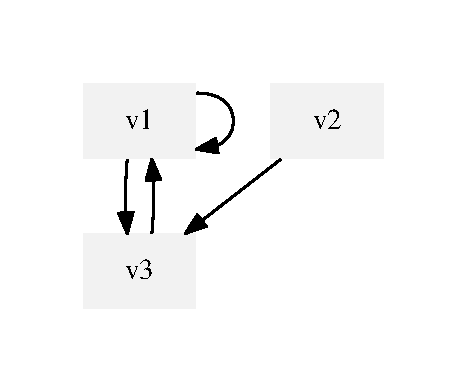
\includegraphics{figure01.pdf}}
\caption{The interaction graph ``\emph{example02\_igraph.pdf}'' of the network defined above.}\label{Manual:figure01}\end{figure}


\subsection{graph, node and edge attributes}
\label{Manual:graph-node-and-edge-attributes}
\emph{PyBoolNet 2.11} generates a \emph{dot} file from an interaction graph by inspecting all its edge, node and graph attributes.
Attributes are just dictionaries that are attached to nodes, edges and the graph itself, see {\hyperref[Installation:installation-networkx]{\emph{NetworkX}}} for an introduction.
Use these attributes to change the appearance of the graph.
The idea is that you either change the appearance of individual nodes and edges using node and edge attributes,
or change their default appearance using graph attributes.
For a list of all available attributes see
\begin{itemize}
\item {} 
\href{http://www.graphviz.org/doc/info/attrs.html}{http://www.graphviz.org/doc/info/attrs.html}.

\end{itemize}

Some node attributes are:
\begin{itemize}
\item {} 
\emph{shape}: sets the shape of the node, e.g. \emph{``rect''}, \emph{``square''}, \emph{``circle''}, \emph{``plaintext''}, \emph{``triangle''}, \emph{``star''}, \emph{``lpromoter''}, \emph{``rpromoter''}

\item {} 
\emph{label} (default is the component name): sets the label of a node

\item {} 
\emph{style}: \emph{``filled''} to fill with a color, \emph{``invis''} to hide or \emph{``''} to revert to default

\item {} 
\emph{fillcolor}: sets the fill color, requires \emph{style=''filled''}

\item {} 
\emph{color}: sets the stroke color

\item {} 
\emph{fontcolor}: sets the font color

\item {} 
\emph{fontsize} (default is \emph{14}): sets the font size in pt, e.g. \emph{5}, \emph{10}, \emph{15}

\item {} 
\emph{fixedsize}: specifies whether the width of a node is fixed, either \emph{``true''} or \emph{``false''}

\item {} 
\emph{width}: sets the node width, e.g. \emph{5}, \emph{10}, \emph{15}

\end{itemize}

Colors can be set by names like \emph{``red''}, \emph{``green''} or \emph{``blue''},
or by space-separated HSV values, e.g. \emph{``0.1 0.2 1.0''},
or by a RGB value, e.g \emph{``\#40e0d0''}.
For a list of predefined color names see for example
\begin{itemize}
\item {} 
\href{http://www.graphviz.org/doc/info/colors.html}{http://www.graphviz.org/doc/info/colors.html}.

\end{itemize}

The basic edge attributes are:
\begin{itemize}
\item {} 
\emph{arrowhead}: sets the shape of the arrow, e.g. \emph{``dot''}, \emph{``tee''}, \emph{``normal''}

\item {} 
\emph{arrowsize}: sets the size of the arrow, e.g. \emph{5}, \emph{10}, \emph{15}

\item {} 
\emph{style}: sets the pen style of the edge, e.g. \emph{``dotted''}, \emph{``dashed''}

\item {} 
\emph{color}: sets the edge color

\item {} 
\emph{label}: sets the label of an edge

\item {} 
\emph{penwidth} (default is \emph{1}): sets the width of an edge, e.g. \emph{5}, \emph{10}, \emph{15}

\item {} 
\emph{constraint} (default is \emph{``true''}): whether the edge should be included in the calculation of the layout, either \emph{``true''} or \emph{``false''}

\item {} 
\emph{weight} (default is \emph{1}): sets the cost for stretching the edge during layout computation, for example \emph{``5''}, \emph{``10''}, \emph{``15''}

\end{itemize}

To set node or edge defaults, add them to the \emph{node} or \emph{edge} attribute of the graph field:

\begin{Verbatim}[commandchars=\\\{\}]
\PYG{g+gp}{\PYGZgt{}\PYGZgt{}\PYGZgt{} }\PYG{n}{bnet} \PYG{o}{=} \PYG{l+s}{\PYGZdq{}}\PYG{l+s+se}{\PYGZbs{}n}\PYG{l+s}{\PYGZdq{}}\PYG{o}{.}\PYG{n}{join}\PYG{p}{(}\PYG{p}{[}\PYG{l+s}{\PYGZdq{}}\PYG{l+s}{v1, v2 \PYGZam{} (!v1 \textbar{} v3)}\PYG{l+s}{\PYGZdq{}}\PYG{p}{,}\PYG{l+s}{\PYGZdq{}}\PYG{l+s}{v2, !v3}\PYG{l+s}{\PYGZdq{}}\PYG{p}{,}\PYG{l+s}{\PYGZdq{}}\PYG{l+s}{v3, v2 \textbar{} v1}\PYG{l+s}{\PYGZdq{}}\PYG{p}{]}\PYG{p}{)}
\PYG{g+gp}{\PYGZgt{}\PYGZgt{}\PYGZgt{} }\PYG{n}{primes} \PYG{o}{=} \PYG{n}{FEX}\PYG{o}{.}\PYG{n}{bnet2primes}\PYG{p}{(}\PYG{n}{bnet}\PYG{p}{)}
\PYG{g+gp}{\PYGZgt{}\PYGZgt{}\PYGZgt{} }\PYG{n}{igraph} \PYG{o}{=} \PYG{n}{IGs}\PYG{o}{.}\PYG{n}{primes2igraph}\PYG{p}{(}\PYG{n}{primes}\PYG{p}{)}
\PYG{g+gp}{\PYGZgt{}\PYGZgt{}\PYGZgt{} }\PYG{n}{igraph}\PYG{o}{.}\PYG{n}{graph}\PYG{p}{[}\PYG{l+s}{\PYGZdq{}}\PYG{l+s}{node}\PYG{l+s}{\PYGZdq{}}\PYG{p}{]}\PYG{p}{[}\PYG{l+s}{\PYGZdq{}}\PYG{l+s}{shape}\PYG{l+s}{\PYGZdq{}}\PYG{p}{]} \PYG{o}{=} \PYG{l+s}{\PYGZdq{}}\PYG{l+s}{circle}\PYG{l+s}{\PYGZdq{}}
\PYG{g+gp}{\PYGZgt{}\PYGZgt{}\PYGZgt{} }\PYG{n}{igraph}\PYG{o}{.}\PYG{n}{graph}\PYG{p}{[}\PYG{l+s}{\PYGZdq{}}\PYG{l+s}{node}\PYG{l+s}{\PYGZdq{}}\PYG{p}{]}\PYG{p}{[}\PYG{l+s}{\PYGZdq{}}\PYG{l+s}{color}\PYG{l+s}{\PYGZdq{}}\PYG{p}{]} \PYG{o}{=} \PYG{l+s}{\PYGZdq{}}\PYG{l+s}{blue}\PYG{l+s}{\PYGZdq{}}
\end{Verbatim}

To change the appearance of specific nodes or edges, add attributes to the node or edge field:

\begin{Verbatim}[commandchars=\\\{\}]
\PYG{g+gp}{\PYGZgt{}\PYGZgt{}\PYGZgt{} }\PYG{n}{igraph}\PYG{o}{.}\PYG{n}{node}\PYG{p}{[}\PYG{l+s}{\PYGZdq{}}\PYG{l+s}{v2}\PYG{l+s}{\PYGZdq{}}\PYG{p}{]}\PYG{p}{[}\PYG{l+s}{\PYGZdq{}}\PYG{l+s}{shape}\PYG{l+s}{\PYGZdq{}}\PYG{p}{]} \PYG{o}{=} \PYG{l+s}{\PYGZdq{}}\PYG{l+s}{rpromoter}\PYG{l+s}{\PYGZdq{}}
\PYG{g+gp}{\PYGZgt{}\PYGZgt{}\PYGZgt{} }\PYG{n}{igraph}\PYG{o}{.}\PYG{n}{node}\PYG{p}{[}\PYG{l+s}{\PYGZdq{}}\PYG{l+s}{v2}\PYG{l+s}{\PYGZdq{}}\PYG{p}{]}\PYG{p}{[}\PYG{l+s}{\PYGZdq{}}\PYG{l+s}{color}\PYG{l+s}{\PYGZdq{}}\PYG{p}{]} \PYG{o}{=} \PYG{l+s}{\PYGZdq{}}\PYG{l+s}{black}\PYG{l+s}{\PYGZdq{}}
\PYG{g+gp}{\PYGZgt{}\PYGZgt{}\PYGZgt{} }\PYG{n}{igraph}\PYG{o}{.}\PYG{n}{edge}\PYG{p}{[}\PYG{l+s}{\PYGZdq{}}\PYG{l+s}{v3}\PYG{l+s}{\PYGZdq{}}\PYG{p}{]}\PYG{p}{[}\PYG{l+s}{\PYGZdq{}}\PYG{l+s}{v1}\PYG{l+s}{\PYGZdq{}}\PYG{p}{]}\PYG{p}{[}\PYG{l+s}{\PYGZdq{}}\PYG{l+s}{arrowhead}\PYG{l+s}{\PYGZdq{}}\PYG{p}{]} \PYG{o}{=} \PYG{l+s}{\PYGZdq{}}\PYG{l+s}{inv}\PYG{l+s}{\PYGZdq{}}
\PYG{g+gp}{\PYGZgt{}\PYGZgt{}\PYGZgt{} }\PYG{n}{igraph}\PYG{o}{.}\PYG{n}{edge}\PYG{p}{[}\PYG{l+s}{\PYGZdq{}}\PYG{l+s}{v3}\PYG{l+s}{\PYGZdq{}}\PYG{p}{]}\PYG{p}{[}\PYG{l+s}{\PYGZdq{}}\PYG{l+s}{v1}\PYG{l+s}{\PYGZdq{}}\PYG{p}{]}\PYG{p}{[}\PYG{l+s}{\PYGZdq{}}\PYG{l+s}{color}\PYG{l+s}{\PYGZdq{}}\PYG{p}{]} \PYG{o}{=} \PYG{l+s}{\PYGZdq{}}\PYG{l+s}{red}\PYG{l+s}{\PYGZdq{}}
\end{Verbatim}

In addition, \emph{dot} graphs have general graph attributes, for example:
\begin{itemize}
\item {} 
\emph{splines}: sets how edges are drawn, e.g. \emph{``line''}, \emph{``curved''} or \emph{``ortho''} for orthogonal edges

\item {} 
\emph{label}: adds a label to the graph

\item {} 
\emph{rankdir} (default is \emph{``TB''}): sets the direction in which layout is constructed, e.g. \emph{``LR''}, \emph{``RL''}, \emph{``BT''}

\end{itemize}

To change graph attributes, add them to the graph dictionary:

\begin{Verbatim}[commandchars=\\\{\}]
\PYG{g+gp}{\PYGZgt{}\PYGZgt{}\PYGZgt{} }\PYG{n}{igraph}\PYG{o}{.}\PYG{n}{graph}\PYG{p}{[}\PYG{l+s}{\PYGZdq{}}\PYG{l+s}{splines}\PYG{l+s}{\PYGZdq{}}\PYG{p}{]} \PYG{o}{=} \PYG{l+s}{\PYGZdq{}}\PYG{l+s}{ortho}\PYG{l+s}{\PYGZdq{}}
\PYG{g+gp}{\PYGZgt{}\PYGZgt{}\PYGZgt{} }\PYG{n}{igraph}\PYG{o}{.}\PYG{n}{graph}\PYG{p}{[}\PYG{l+s}{\PYGZdq{}}\PYG{l+s}{rankdir}\PYG{l+s}{\PYGZdq{}}\PYG{p}{]} \PYG{o}{=} \PYG{l+s}{\PYGZdq{}}\PYG{l+s}{LR}\PYG{l+s}{\PYGZdq{}}
\PYG{g+gp}{\PYGZgt{}\PYGZgt{}\PYGZgt{} }\PYG{n}{igraph}\PYG{o}{.}\PYG{n}{graph}\PYG{p}{[}\PYG{l+s}{\PYGZdq{}}\PYG{l+s}{label}\PYG{l+s}{\PYGZdq{}}\PYG{p}{]} \PYG{o}{=} \PYG{l+s}{\PYGZdq{}}\PYG{l+s}{Example 3: Interaction graph with attributes}\PYG{l+s}{\PYGZdq{}}
\PYG{g+gp}{\PYGZgt{}\PYGZgt{}\PYGZgt{} }\PYG{n}{IGs}\PYG{o}{.}\PYG{n}{igraph2image}\PYG{p}{(}\PYG{n}{igraph}\PYG{p}{,} \PYG{l+s}{\PYGZdq{}}\PYG{l+s}{example03\PYGZus{}igraph.pdf}\PYG{l+s}{\PYGZdq{}}\PYG{p}{)}
\end{Verbatim}

The result is shown in {\hyperref[Manual:figure02]{\emph{the figure below}}}.
\begin{figure}[htbp]
\centering
\capstart

\scalebox{0.600000}{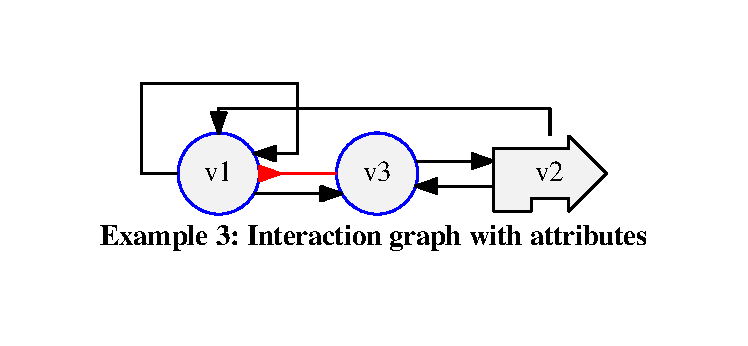
\includegraphics{figure02.pdf}}
\caption{The interaction graph ``\emph{example03\_igraph.pdf}''.}\label{Manual:figure02}\end{figure}


\subsection{the interaction signs style}
\label{Manual:the-interaction-signs-style}
\emph{PyBoolNet 2.11} has predefined styles for adding attributes to interaction graphs.
The function {\hyperref[InteractionGraphs:add-style-interactionsigns]{\emph{add\_style\_interactionsigns}}} adds or overwrites color and arrowhead attributes to indicate whether an interaction is activating, inhibiting or both.
Activating interactions are black with normal arrowheads,
inhibiting interactions are red with blunt arrowhead and
interactions that are both activating and inhibiting are blue with round arrowheads.

Consider a network with a \emph{exclusive or} regulation:

\begin{Verbatim}[commandchars=\\\{\}]
\PYG{g+gp}{\PYGZgt{}\PYGZgt{}\PYGZgt{} }\PYG{n}{funcs} \PYG{o}{=} \PYG{p}{\PYGZob{}}\PYG{l+s}{\PYGZdq{}}\PYG{l+s}{v1}\PYG{l+s}{\PYGZdq{}}\PYG{p}{:}\PYG{k}{lambda} \PYG{n}{v1}\PYG{p}{,}\PYG{n}{v2}\PYG{p}{,}\PYG{n}{v3}\PYG{p}{:} \PYG{n}{v1}\PYG{o}{+}\PYG{n}{v2}\PYG{o}{+}\PYG{n}{v3}\PYG{o}{==}\PYG{l+m+mi}{1}\PYG{p}{,}
\PYG{g+gp}{... }         \PYG{l+s}{\PYGZdq{}}\PYG{l+s}{v2}\PYG{l+s}{\PYGZdq{}}\PYG{p}{:}\PYG{k}{lambda} \PYG{n}{v1}\PYG{p}{:} \PYG{o+ow}{not} \PYG{n}{v1}\PYG{p}{,}
\PYG{g+gp}{... }         \PYG{l+s}{\PYGZdq{}}\PYG{l+s}{v3}\PYG{l+s}{\PYGZdq{}}\PYG{p}{:}\PYG{k}{lambda} \PYG{n}{v2}\PYG{p}{:} \PYG{n}{v2}\PYG{p}{\PYGZcb{}}
\PYG{g+gp}{\PYGZgt{}\PYGZgt{}\PYGZgt{} }\PYG{n}{primes} \PYG{o}{=} \PYG{n}{QMC}\PYG{o}{.}\PYG{n}{functions2primes}\PYG{p}{(}\PYG{n}{funcs}\PYG{p}{)}
\PYG{g+gp}{\PYGZgt{}\PYGZgt{}\PYGZgt{} }\PYG{n}{igraph} \PYG{o}{=} \PYG{n}{IGs}\PYG{o}{.}\PYG{n}{primes2igraph}\PYG{p}{(}\PYG{n}{primes}\PYG{p}{)}
\PYG{g+gp}{\PYGZgt{}\PYGZgt{}\PYGZgt{} }\PYG{n}{IGs}\PYG{o}{.}\PYG{n}{add\PYGZus{}style\PYGZus{}interactionsigns}\PYG{p}{(}\PYG{n}{igraph}\PYG{p}{)}
\PYG{g+gp}{\PYGZgt{}\PYGZgt{}\PYGZgt{} }\PYG{n}{igraph}\PYG{o}{.}\PYG{n}{graph}\PYG{p}{[}\PYG{l+s}{\PYGZdq{}}\PYG{l+s}{label}\PYG{l+s}{\PYGZdq{}}\PYG{p}{]} \PYG{o}{=} \PYG{l+s}{\PYGZdq{}}\PYG{l+s}{Example 4: Signed interaction graph}\PYG{l+s}{\PYGZdq{}}
\PYG{g+gp}{\PYGZgt{}\PYGZgt{}\PYGZgt{} }\PYG{n}{igraph}\PYG{o}{.}\PYG{n}{graph}\PYG{p}{[}\PYG{l+s}{\PYGZdq{}}\PYG{l+s}{rankdir}\PYG{l+s}{\PYGZdq{}}\PYG{p}{]} \PYG{o}{=} \PYG{l+s}{\PYGZdq{}}\PYG{l+s}{LR}\PYG{l+s}{\PYGZdq{}}
\PYG{g+gp}{\PYGZgt{}\PYGZgt{}\PYGZgt{} }\PYG{n}{IGs}\PYG{o}{.}\PYG{n}{igraph2image}\PYG{p}{(}\PYG{n}{igraph}\PYG{p}{,} \PYG{l+s}{\PYGZdq{}}\PYG{l+s}{example04\PYGZus{}igraph.pdf}\PYG{l+s}{\PYGZdq{}}\PYG{p}{)}
\end{Verbatim}

The result is shown in {\hyperref[Manual:figure03]{\emph{the figure below}}}.
\begin{figure}[htbp]
\centering
\capstart

\scalebox{0.600000}{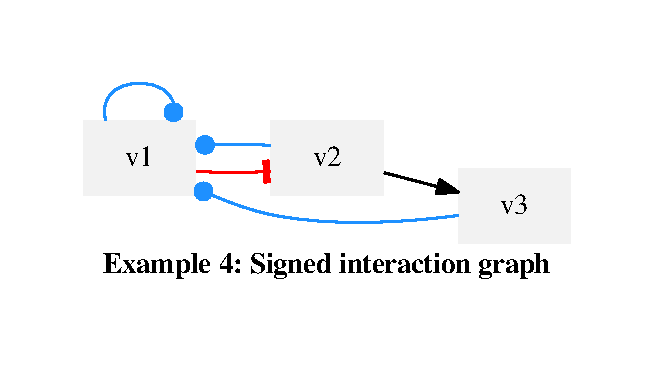
\includegraphics{figure03.pdf}}
\caption{The interaction graph ``\emph{example04\_igraph.pdf}'' with attributes added by \emph{add\_style\_interactionsings}.}\label{Manual:figure03}\end{figure}


\subsection{styles for inputs, outputs and constants}
\label{Manual:styles-for-inputs-outputs-and-constants}
\emph{Inputs} are components that are only regulated by themselves.
Usually, inputs regulate themselves positively but we also consider inputs that regulate themselves negatively as inputs.
\emph{Outputs} are components that do not regulate other components and \emph{constants} are components whose update function is constant and always returns either \emph{True} or \emph{False}.

To highlight inputs and outputs by grouping them inside a box use the functions {\hyperref[InteractionGraphs:add-style-inputs]{\emph{add\_style\_inputs}}} and {\hyperref[InteractionGraphs:add-style-outputs]{\emph{add\_style\_outputs}}}.
They add \emph{dot} subgraphs that contain all components of the respective type and add the label \emph{``inputs''} or \emph{``outputs''}.
The function {\hyperref[InteractionGraphs:add-style-constants]{\emph{add\_style\_constants}}} changes the shape of constants to \emph{``plaintext''},
their font to \emph{``Time-Italic''} and the color of all interactions involving constants to \emph{``gray''}.

Consider this example:

\begin{Verbatim}[commandchars=\\\{\}]
\PYG{g+gp}{\PYGZgt{}\PYGZgt{}\PYGZgt{} }\PYG{n}{bnet} \PYG{o}{=} \PYG{p}{[}\PYG{l+s}{\PYGZdq{}}\PYG{l+s}{v1, v1}\PYG{l+s}{\PYGZdq{}}\PYG{p}{,} \PYG{l+s}{\PYGZdq{}}\PYG{l+s}{v2, v2}\PYG{l+s}{\PYGZdq{}}\PYG{p}{,} \PYG{l+s}{\PYGZdq{}}\PYG{l+s}{v3, 1}\PYG{l+s}{\PYGZdq{}}\PYG{p}{,} \PYG{l+s}{\PYGZdq{}}\PYG{l+s}{v4, v1 \textbar{} v3}\PYG{l+s}{\PYGZdq{}}\PYG{p}{,}
\PYG{g+gp}{... }        \PYG{l+s}{\PYGZdq{}}\PYG{l+s}{v5, v4 \PYGZam{} v2 \textbar{} v6}\PYG{l+s}{\PYGZdq{}}\PYG{p}{,} \PYG{l+s}{\PYGZdq{}}\PYG{l+s}{v6, 0}\PYG{l+s}{\PYGZdq{}}\PYG{p}{,} \PYG{l+s}{\PYGZdq{}}\PYG{l+s}{v7, !v5}\PYG{l+s}{\PYGZdq{}}\PYG{p}{,}
\PYG{g+gp}{... }        \PYG{l+s}{\PYGZdq{}}\PYG{l+s}{v8, v7}\PYG{l+s}{\PYGZdq{}}\PYG{p}{,} \PYG{l+s}{\PYGZdq{}}\PYG{l+s}{v9, v5 \PYGZam{} v7}\PYG{l+s}{\PYGZdq{}}\PYG{p}{]}
\PYG{g+gp}{\PYGZgt{}\PYGZgt{}\PYGZgt{} }\PYG{n}{bnet} \PYG{o}{=} \PYG{l+s}{\PYGZdq{}}\PYG{l+s+se}{\PYGZbs{}n}\PYG{l+s}{\PYGZdq{}}\PYG{o}{.}\PYG{n}{join}\PYG{p}{(}\PYG{n}{bnet}\PYG{p}{)}
\PYG{g+gp}{\PYGZgt{}\PYGZgt{}\PYGZgt{} }\PYG{n}{primes} \PYG{o}{=} \PYG{n}{FEX}\PYG{o}{.}\PYG{n}{bnet2primes}\PYG{p}{(}\PYG{n}{bnet}\PYG{p}{)}
\PYG{g+gp}{\PYGZgt{}\PYGZgt{}\PYGZgt{} }\PYG{n}{igraph} \PYG{o}{=} \PYG{n}{IGs}\PYG{o}{.}\PYG{n}{primes2igraph}\PYG{p}{(}\PYG{n}{primes}\PYG{p}{)}
\PYG{g+gp}{\PYGZgt{}\PYGZgt{}\PYGZgt{} }\PYG{n}{IGs}\PYG{o}{.}\PYG{n}{add\PYGZus{}style\PYGZus{}inputs}\PYG{p}{(}\PYG{n}{igraph}\PYG{p}{)}
\PYG{g+gp}{\PYGZgt{}\PYGZgt{}\PYGZgt{} }\PYG{n}{IGs}\PYG{o}{.}\PYG{n}{add\PYGZus{}style\PYGZus{}constants}\PYG{p}{(}\PYG{n}{igraph}\PYG{p}{)}
\PYG{g+gp}{\PYGZgt{}\PYGZgt{}\PYGZgt{} }\PYG{n}{IGs}\PYG{o}{.}\PYG{n}{add\PYGZus{}style\PYGZus{}outputs}\PYG{p}{(}\PYG{n}{igraph}\PYG{p}{)}
\PYG{g+gp}{\PYGZgt{}\PYGZgt{}\PYGZgt{} }\PYG{n}{igraph}\PYG{o}{.}\PYG{n}{graph}\PYG{p}{[}\PYG{l+s}{\PYGZdq{}}\PYG{l+s}{label}\PYG{l+s}{\PYGZdq{}}\PYG{p}{]} \PYG{o}{=} \PYG{l+s}{\PYGZdq{}}\PYG{l+s}{Example 5: Interaction graph with styles for}\PYG{l+s}{\PYGZdq{}}\PYG{o}{+}
\PYG{g+gp}{... }                        \PYG{l+s}{\PYGZdq{}}\PYG{l+s}{inputs, outputs and constants}\PYG{l+s}{\PYGZdq{}}
\PYG{g+gp}{\PYGZgt{}\PYGZgt{}\PYGZgt{} }\PYG{n}{IGs}\PYG{o}{.}\PYG{n}{igraph2image}\PYG{p}{(}\PYG{n}{igraph}\PYG{p}{,} \PYG{l+s}{\PYGZdq{}}\PYG{l+s}{example05\PYGZus{}igraph.pdf}\PYG{l+s}{\PYGZdq{}}\PYG{p}{)}
\end{Verbatim}

The result is shown in {\hyperref[Manual:figure04]{\emph{the figure below}}}.
\begin{figure}[htbp]
\centering
\capstart

\scalebox{0.600000}{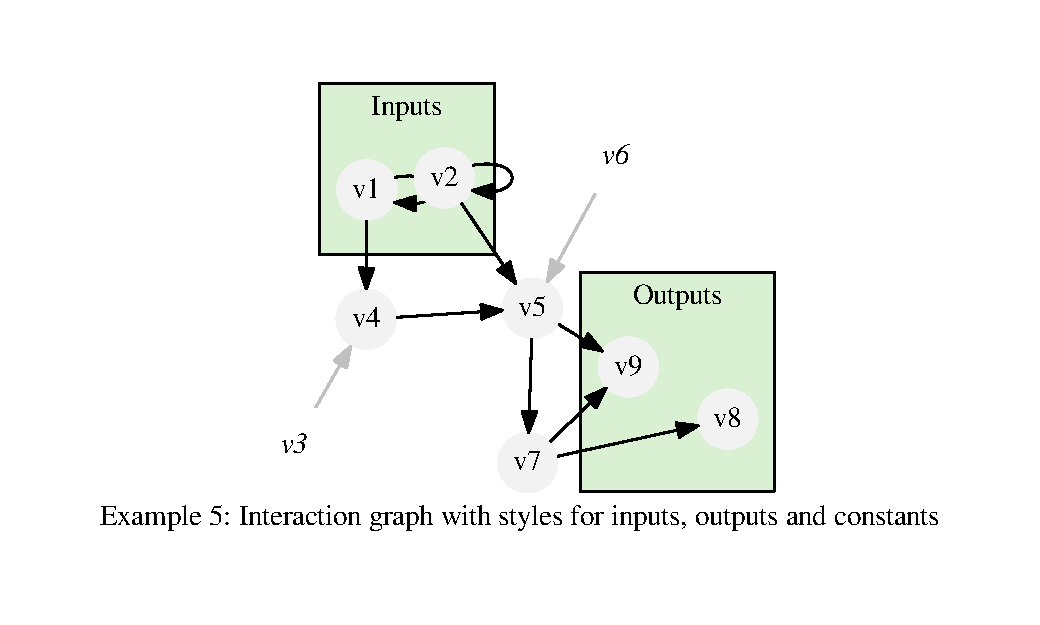
\includegraphics{figure04.pdf}}
\caption{The interaction graph ``\emph{example05.pdf}'' with styles added by {\hyperref[InteractionGraphs:add-style-inputs]{\emph{add\_style\_inputs}}}, {\hyperref[InteractionGraphs:add-style-outputs]{\emph{add\_style\_outputs}}} and {\hyperref[InteractionGraphs:add-style-constants]{\emph{add\_style\_constants}}}.}\label{Manual:figure04}\end{figure}


\subsection{the SCCs style}
\label{Manual:the-sccs-style}
The function {\hyperref[StateTransitionGraphs:add-style-sccs]{\emph{add\_style\_sccs}}} defines a \emph{dot} subgraph for every non-trivial \emph{strongly connected component} (SCC) of the interaction graph.
Each SCC subgraph is filled by a shade of gray that indicates the longest path of SCCs leading to it,
a unique number that intuitively represents ``the depth in the SCC hierarchy'', see {\hyperref[Bibliography:klarner2015approx]{\emph{Klarner2015(b)}}} for a formal definition.
The further down the hierarchy, the darker the shade of gray will be.
Shades of gray repeat after a depth of nine.

Consider the network:

\begin{Verbatim}[commandchars=\\\{\}]
\PYG{g+gp}{\PYGZgt{}\PYGZgt{}\PYGZgt{} }\PYG{n}{bnet} \PYG{o}{=} \PYG{p}{[}\PYG{l+s}{\PYGZdq{}}\PYG{l+s}{v1, v1}\PYG{l+s}{\PYGZdq{}}\PYG{p}{,} \PYG{l+s}{\PYGZdq{}}\PYG{l+s}{v2, v3 \PYGZam{} v5}\PYG{l+s}{\PYGZdq{}}\PYG{p}{,} \PYG{l+s}{\PYGZdq{}}\PYG{l+s}{v3, v1}\PYG{l+s}{\PYGZdq{}}\PYG{p}{,} \PYG{l+s}{\PYGZdq{}}\PYG{l+s}{v4, v1}\PYG{l+s}{\PYGZdq{}}\PYG{p}{,} \PYG{l+s}{\PYGZdq{}}\PYG{l+s}{v5, 1}\PYG{l+s}{\PYGZdq{}}\PYG{p}{,}
\PYG{g+gp}{... }        \PYG{l+s}{\PYGZdq{}}\PYG{l+s}{v6, v7}\PYG{l+s}{\PYGZdq{}}\PYG{p}{,} \PYG{l+s}{\PYGZdq{}}\PYG{l+s}{v7, v6 \textbar{} v4}\PYG{l+s}{\PYGZdq{}}\PYG{p}{,} \PYG{l+s}{\PYGZdq{}}\PYG{l+s}{v8, v6}\PYG{l+s}{\PYGZdq{}}\PYG{p}{,} \PYG{l+s}{\PYGZdq{}}\PYG{l+s}{v9, v8}\PYG{l+s}{\PYGZdq{}}\PYG{p}{,} \PYG{l+s}{\PYGZdq{}}\PYG{l+s}{v10, v7 \PYGZam{} v11}\PYG{l+s}{\PYGZdq{}}\PYG{p}{,}
\PYG{g+gp}{... }        \PYG{l+s}{\PYGZdq{}}\PYG{l+s}{v11, v10 \textbar{} v4}\PYG{l+s}{\PYGZdq{}}\PYG{p}{,} \PYG{l+s}{\PYGZdq{}}\PYG{l+s}{v12, v10}\PYG{l+s}{\PYGZdq{}}\PYG{p}{]}
\PYG{g+gp}{\PYGZgt{}\PYGZgt{}\PYGZgt{} }\PYG{n}{bnet} \PYG{o}{=} \PYG{l+s}{\PYGZdq{}}\PYG{l+s+se}{\PYGZbs{}n}\PYG{l+s}{\PYGZdq{}}\PYG{o}{.}\PYG{n}{join}\PYG{p}{(}\PYG{n}{bnet}\PYG{p}{)}
\PYG{g+gp}{\PYGZgt{}\PYGZgt{}\PYGZgt{} }\PYG{n}{primes} \PYG{o}{=} \PYG{n}{FEX}\PYG{o}{.}\PYG{n}{bnet2primes}\PYG{p}{(}\PYG{n}{bnet}\PYG{p}{)}
\PYG{g+gp}{\PYGZgt{}\PYGZgt{}\PYGZgt{} }\PYG{n}{igraph} \PYG{o}{=} \PYG{n}{IGs}\PYG{o}{.}\PYG{n}{primes2igraph}\PYG{p}{(}\PYG{n}{primes}\PYG{p}{)}
\PYG{g+gp}{\PYGZgt{}\PYGZgt{}\PYGZgt{} }\PYG{n}{IGs}\PYG{o}{.}\PYG{n}{add\PYGZus{}style\PYGZus{}sccs}\PYG{p}{(}\PYG{n}{igraph}\PYG{p}{)}
\PYG{g+gp}{\PYGZgt{}\PYGZgt{}\PYGZgt{} }\PYG{n}{igraph}\PYG{o}{.}\PYG{n}{graph}\PYG{p}{[}\PYG{l+s}{\PYGZdq{}}\PYG{l+s}{label}\PYG{l+s}{\PYGZdq{}}\PYG{p}{]} \PYG{o}{=} \PYG{l+s}{\PYGZdq{}}\PYG{l+s}{Example 6: Interaction graph with SCC style}\PYG{l+s}{\PYGZdq{}}
\PYG{g+gp}{\PYGZgt{}\PYGZgt{}\PYGZgt{} }\PYG{n}{IGs}\PYG{o}{.}\PYG{n}{igraph2image}\PYG{p}{(}\PYG{n}{igraph}\PYG{p}{,} \PYG{l+s}{\PYGZdq{}}\PYG{l+s}{example06\PYGZus{}igraph.pdf}\PYG{l+s}{\PYGZdq{}}\PYG{p}{)}
\end{Verbatim}

The result is shown in {\hyperref[Manual:figure05]{\emph{the figure below}}}.
\begin{figure}[htbp]
\centering
\capstart

\scalebox{0.600000}{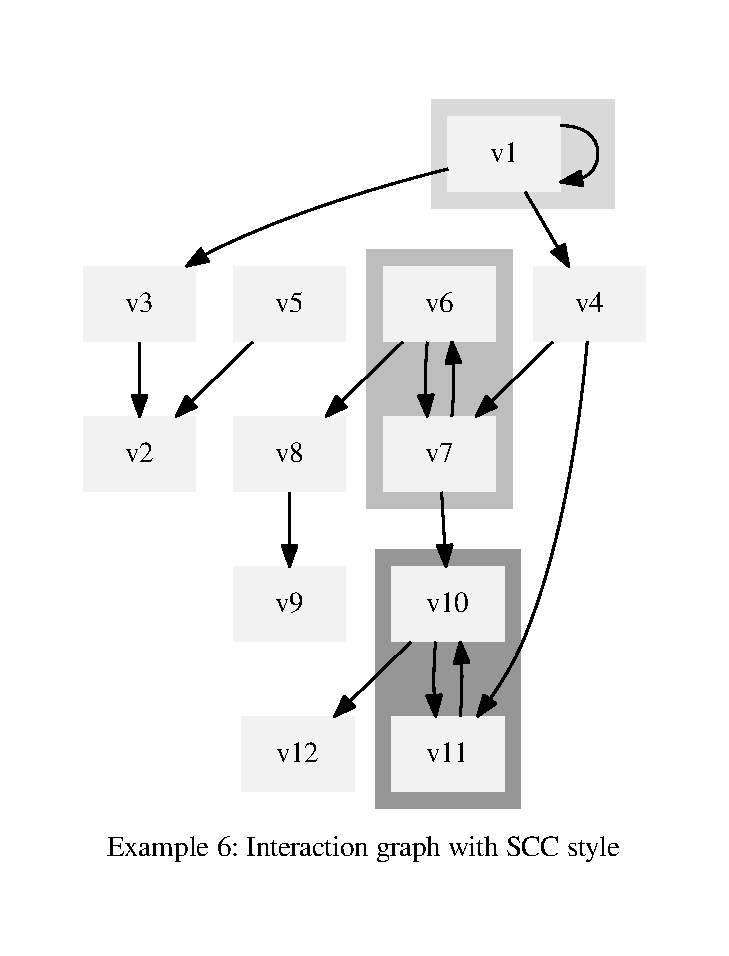
\includegraphics{figure05.pdf}}
\caption{The interaction graph ``\emph{example06\_igraph.pdf}'' with attributes added by {\hyperref[StateTransitionGraphs:add-style-sccs]{\emph{add\_style\_sccs}}}.}\label{Manual:figure05}\end{figure}


\subsection{the subgraphs style}
\label{Manual:the-subgraphs-style}
The function {\hyperref[StateTransitionGraphs:add-style-subgraphs]{\emph{add\_style\_subgraphs}}} allows you to specify subsets of nodes that will be added to a \emph{dot} subgraph.
The subgraphs may be specified as a list of pairs that consist of a list of names and a dictionary
of \emph{dot} attributes for that subgraph, e.g., a label or background color.

\begin{notice}{note}{Note:}
\emph{Subgraphs} must satisfy this property:
Any two subgraphs have either empty intersection or one is a subset of the other.
The reason for this requirement is that \emph{dot} can not draw intersecting subgraphs.
\end{notice}

Consider the network:

\begin{Verbatim}[commandchars=\\\{\}]
\PYG{g+gp}{\PYGZgt{}\PYGZgt{}\PYGZgt{} }\PYG{n}{bnet} \PYG{o}{=} \PYG{p}{[}\PYG{l+s}{\PYGZdq{}}\PYG{l+s}{v1, v7}\PYG{l+s}{\PYGZdq{}}\PYG{p}{,} \PYG{l+s}{\PYGZdq{}}\PYG{l+s}{v2, v1 \PYGZam{} v6}\PYG{l+s}{\PYGZdq{}}\PYG{p}{,} \PYG{l+s}{\PYGZdq{}}\PYG{l+s}{v3, v2 \textbar{} v7}\PYG{l+s}{\PYGZdq{}}\PYG{p}{,} \PYG{l+s}{\PYGZdq{}}\PYG{l+s}{v4, v3}\PYG{l+s}{\PYGZdq{}}\PYG{p}{,}
\PYG{g+gp}{... }        \PYG{l+s}{\PYGZdq{}}\PYG{l+s}{v5, v1 \textbar{} v4}\PYG{l+s}{\PYGZdq{}}\PYG{p}{,} \PYG{l+s}{\PYGZdq{}}\PYG{l+s}{v6, v5}\PYG{l+s}{\PYGZdq{}}\PYG{p}{,} \PYG{l+s}{\PYGZdq{}}\PYG{l+s}{v7, v6}\PYG{l+s}{\PYGZdq{}}\PYG{p}{]}
\PYG{g+gp}{\PYGZgt{}\PYGZgt{}\PYGZgt{} }\PYG{n}{bnet} \PYG{o}{=} \PYG{l+s}{\PYGZdq{}}\PYG{l+s+se}{\PYGZbs{}n}\PYG{l+s}{\PYGZdq{}}\PYG{o}{.}\PYG{n}{join}\PYG{p}{(}\PYG{n}{bnet}\PYG{p}{)}
\PYG{g+gp}{\PYGZgt{}\PYGZgt{}\PYGZgt{} }\PYG{n}{primes} \PYG{o}{=} \PYG{n}{FEX}\PYG{o}{.}\PYG{n}{bnet2primes}\PYG{p}{(}\PYG{n}{bnet}\PYG{p}{)}
\PYG{g+gp}{\PYGZgt{}\PYGZgt{}\PYGZgt{} }\PYG{n}{igraph} \PYG{o}{=} \PYG{n}{IGs}\PYG{o}{.}\PYG{n}{primes2igraph}\PYG{p}{(}\PYG{n}{primes}\PYG{p}{)}
\PYG{g+gp}{\PYGZgt{}\PYGZgt{}\PYGZgt{} }\PYG{n}{subgraphs} \PYG{o}{=} \PYG{p}{[}\PYG{p}{(}\PYG{p}{[}\PYG{l+s}{\PYGZdq{}}\PYG{l+s}{v2}\PYG{l+s}{\PYGZdq{}}\PYG{p}{,}\PYG{l+s}{\PYGZdq{}}\PYG{l+s}{v6}\PYG{l+s}{\PYGZdq{}}\PYG{p}{]}\PYG{p}{,}\PYG{p}{\PYGZob{}}\PYG{p}{\PYGZcb{}}\PYG{p}{)}\PYG{p}{,}
\PYG{g+gp}{... }             \PYG{p}{(}\PYG{p}{[}\PYG{l+s}{\PYGZdq{}}\PYG{l+s}{v1}\PYG{l+s}{\PYGZdq{}}\PYG{p}{,}\PYG{l+s}{\PYGZdq{}}\PYG{l+s}{v4}\PYG{l+s}{\PYGZdq{}}\PYG{p}{]}\PYG{p}{,}\PYG{p}{\PYGZob{}}\PYG{l+s}{\PYGZdq{}}\PYG{l+s}{label}\PYG{l+s}{\PYGZdq{}}\PYG{p}{:}\PYG{l+s}{\PYGZdq{}}\PYG{l+s}{Genes}\PYG{l+s}{\PYGZdq{}}\PYG{p}{,} \PYG{l+s}{\PYGZdq{}}\PYG{l+s}{fillcolor}\PYG{l+s}{\PYGZdq{}}\PYG{p}{:}\PYG{l+s}{\PYGZdq{}}\PYG{l+s}{lightblue}\PYG{l+s}{\PYGZdq{}}\PYG{p}{\PYGZcb{}}\PYG{p}{)}\PYG{p}{]}
\PYG{g+gp}{\PYGZgt{}\PYGZgt{}\PYGZgt{} }\PYG{n}{IGs}\PYG{o}{.}\PYG{n}{add\PYGZus{}style\PYGZus{}subgraphs}\PYG{p}{(}\PYG{n}{igraph}\PYG{p}{,} \PYG{n}{subgraphs}\PYG{p}{)}
\PYG{g+gp}{\PYGZgt{}\PYGZgt{}\PYGZgt{} }\PYG{n}{igraph}\PYG{o}{.}\PYG{n}{graph}\PYG{p}{[}\PYG{l+s}{\PYGZdq{}}\PYG{l+s}{label}\PYG{l+s}{\PYGZdq{}}\PYG{p}{]} \PYG{o}{=} \PYG{l+s}{\PYGZdq{}}\PYG{l+s}{Example 8: Interaction graph with a subgraph style}\PYG{l+s}{\PYGZdq{}}
\PYG{g+gp}{\PYGZgt{}\PYGZgt{}\PYGZgt{} }\PYG{n}{IGs}\PYG{o}{.}\PYG{n}{igraph2image}\PYG{p}{(}\PYG{n}{igraph}\PYG{p}{,} \PYG{l+s}{\PYGZdq{}}\PYG{l+s}{example08\PYGZus{}igraph.pdf}\PYG{l+s}{\PYGZdq{}}\PYG{p}{)}
\end{Verbatim}

The result is shown in {\hyperref[Manual:figure07]{\emph{the figure below}}}.
\begin{figure}[htbp]
\centering
\capstart

\scalebox{0.600000}{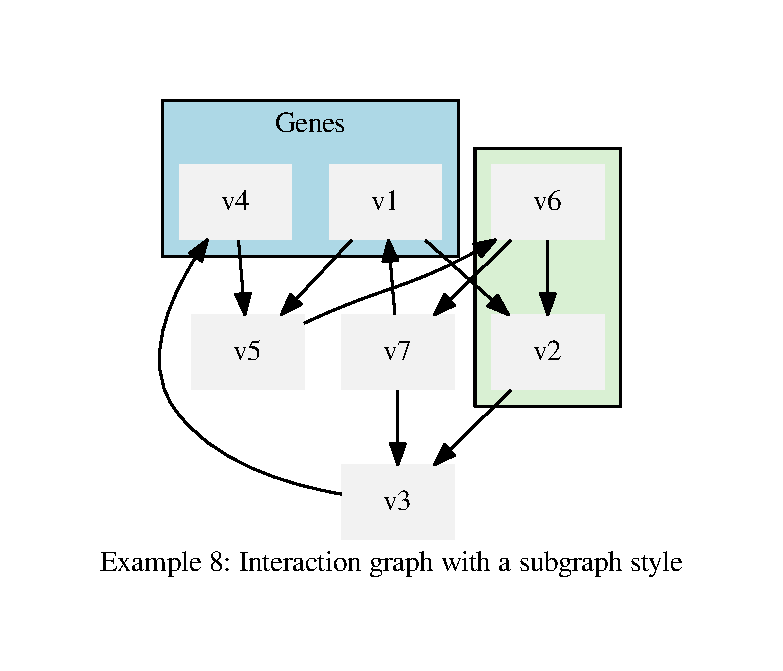
\includegraphics{figure07.pdf}}
\caption{The interaction graph ``\emph{example08\_igraph.pdf}'' with attributes added by {\hyperref[StateTransitionGraphs:add-style-subgraphs]{\emph{add\_style\_subgraphs}}}.}\label{Manual:figure07}\end{figure}


\subsection{the activities style and animations}
\label{Manual:the-activities-style-and-animations}
The function {\hyperref[InteractionGraphs:add-style-activities]{\emph{add\_style\_activities}}} colors components according to a given dictionary of activities, i.e., a state or subspace.
Components that are active are colored in red, inactive ones blue and the attributes of the remaining components are not changed.
In addition, interactions that involve activated or inhibited components are grayed out to reflect that they are ineffective.

Here is an example:

\begin{Verbatim}[commandchars=\\\{\}]
\PYG{g+gp}{\PYGZgt{}\PYGZgt{}\PYGZgt{} }\PYG{n}{bnet} \PYG{o}{=} \PYG{p}{[}\PYG{l+s}{\PYGZdq{}}\PYG{l+s}{v1, v7}\PYG{l+s}{\PYGZdq{}}\PYG{p}{,} \PYG{l+s}{\PYGZdq{}}\PYG{l+s}{v2, v1 \PYGZam{} v6}\PYG{l+s}{\PYGZdq{}}\PYG{p}{,} \PYG{l+s}{\PYGZdq{}}\PYG{l+s}{v3, v2 \textbar{} v7}\PYG{l+s}{\PYGZdq{}}\PYG{p}{,} \PYG{l+s}{\PYGZdq{}}\PYG{l+s}{v4, v3}\PYG{l+s}{\PYGZdq{}}\PYG{p}{,}
\PYG{g+gp}{... }        \PYG{l+s}{\PYGZdq{}}\PYG{l+s}{v5, v1 \textbar{} v4}\PYG{l+s}{\PYGZdq{}}\PYG{p}{,} \PYG{l+s}{\PYGZdq{}}\PYG{l+s}{v6, v5}\PYG{l+s}{\PYGZdq{}}\PYG{p}{,} \PYG{l+s}{\PYGZdq{}}\PYG{l+s}{v7, v6}\PYG{l+s}{\PYGZdq{}}\PYG{p}{]}
\PYG{g+gp}{\PYGZgt{}\PYGZgt{}\PYGZgt{} }\PYG{n}{bnet} \PYG{o}{=} \PYG{l+s}{\PYGZdq{}}\PYG{l+s+se}{\PYGZbs{}n}\PYG{l+s}{\PYGZdq{}}\PYG{o}{.}\PYG{n}{join}\PYG{p}{(}\PYG{n}{bnet}\PYG{p}{)}
\PYG{g+gp}{\PYGZgt{}\PYGZgt{}\PYGZgt{} }\PYG{n}{primes} \PYG{o}{=} \PYG{n}{FEX}\PYG{o}{.}\PYG{n}{bnet2primes}\PYG{p}{(}\PYG{n}{bnet}\PYG{p}{)}
\PYG{g+gp}{\PYGZgt{}\PYGZgt{}\PYGZgt{} }\PYG{n}{igraph} \PYG{o}{=} \PYG{n}{IGs}\PYG{o}{.}\PYG{n}{primes2igraph}\PYG{p}{(}\PYG{n}{primes}\PYG{p}{)}
\PYG{g+gp}{\PYGZgt{}\PYGZgt{}\PYGZgt{} }\PYG{n}{activities} \PYG{o}{=} \PYG{p}{\PYGZob{}}\PYG{l+s}{\PYGZdq{}}\PYG{l+s}{v2}\PYG{l+s}{\PYGZdq{}}\PYG{p}{:}\PYG{l+m+mi}{1}\PYG{p}{,} \PYG{l+s}{\PYGZdq{}}\PYG{l+s}{v3}\PYG{l+s}{\PYGZdq{}}\PYG{p}{:}\PYG{l+m+mi}{0}\PYG{p}{,} \PYG{l+s}{\PYGZdq{}}\PYG{l+s}{v4}\PYG{l+s}{\PYGZdq{}}\PYG{p}{:}\PYG{l+m+mi}{0}\PYG{p}{\PYGZcb{}}
\PYG{g+gp}{\PYGZgt{}\PYGZgt{}\PYGZgt{} }\PYG{n}{IGs}\PYG{o}{.}\PYG{n}{add\PYGZus{}style\PYGZus{}activities}\PYG{p}{(}\PYG{n}{igraph}\PYG{p}{,} \PYG{n}{activities}\PYG{p}{)}
\PYG{g+gp}{\PYGZgt{}\PYGZgt{}\PYGZgt{} }\PYG{n}{igraph}\PYG{o}{.}\PYG{n}{graph}\PYG{p}{[}\PYG{l+s}{\PYGZdq{}}\PYG{l+s}{label}\PYG{l+s}{\PYGZdq{}}\PYG{p}{]} \PYG{o}{=} \PYG{l+s}{\PYGZdq{}}\PYG{l+s}{Example 9: Interaction graph with a activities style}\PYG{l+s}{\PYGZdq{}}
\PYG{g+gp}{\PYGZgt{}\PYGZgt{}\PYGZgt{} }\PYG{n}{igraph}\PYG{o}{.}\PYG{n}{graph}\PYG{p}{[}\PYG{l+s}{\PYGZdq{}}\PYG{l+s}{rankdir}\PYG{l+s}{\PYGZdq{}}\PYG{p}{]} \PYG{o}{=} \PYG{l+s}{\PYGZdq{}}\PYG{l+s}{LR}\PYG{l+s}{\PYGZdq{}}
\PYG{g+gp}{\PYGZgt{}\PYGZgt{}\PYGZgt{} }\PYG{n}{IGs}\PYG{o}{.}\PYG{n}{igraph2image}\PYG{p}{(}\PYG{n}{igraph}\PYG{p}{,} \PYG{l+s}{\PYGZdq{}}\PYG{l+s}{example09\PYGZus{}igraph.pdf}\PYG{l+s}{\PYGZdq{}}\PYG{p}{)}
\end{Verbatim}

The result is shown in {\hyperref[Manual:figure08]{\emph{the figure below}}}.
\begin{figure}[htbp]
\centering
\capstart

\scalebox{0.800000}{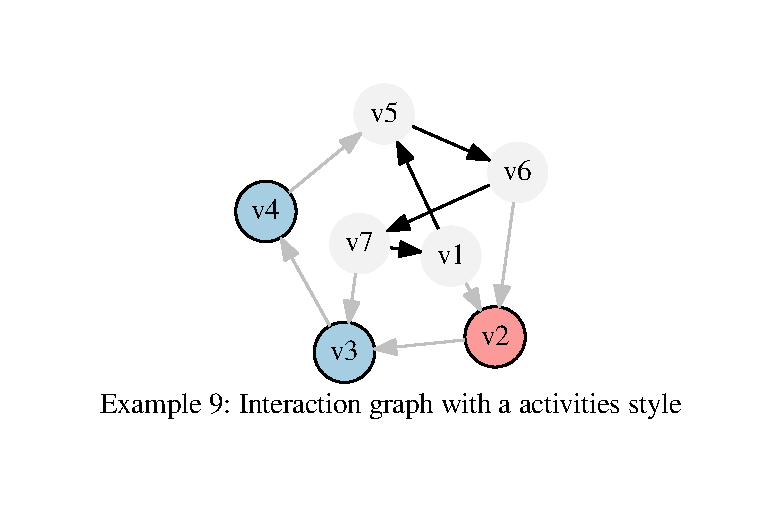
\includegraphics{figure08.pdf}}
\caption{The interaction graph ``\emph{example09\_igraph.pdf}'' with attributes added by {\hyperref[InteractionGraphs:add-style-activities]{\emph{add\_style\_activities}}}.}\label{Manual:figure08}\end{figure}

You can also create an animated \emph{gif} from an interaction graph and a sequence of activities.
Note that as mentioned in {\hyperref[Manual:states-subspaces-paths]{\emph{states, subspaces and paths}}}, activities may be given as strings that consist of 0s, 1s and dashes
using the function {\hyperref[InteractionGraphs:activities2animation]{\emph{activities2animation}}}:

\begin{Verbatim}[commandchars=\\\{\}]
\PYG{g+gp}{\PYGZgt{}\PYGZgt{}\PYGZgt{} }\PYG{n}{activities} \PYG{o}{=} \PYG{p}{[}\PYG{l+s}{\PYGZdq{}}\PYG{l+s}{\PYGZhy{}100}\PYG{l+s}{\PYGZdq{}}\PYG{p}{,} \PYG{l+s}{\PYGZdq{}}\PYG{l+s}{\PYGZhy{}110}\PYG{l+s}{\PYGZdq{}}\PYG{p}{,} \PYG{l+s}{\PYGZdq{}}\PYG{l+s}{\PYGZhy{}010}\PYG{l+s}{\PYGZdq{}}\PYG{p}{]}
\PYG{g+gp}{\PYGZgt{}\PYGZgt{}\PYGZgt{} }\PYG{n}{IGs}\PYG{o}{.}\PYG{n}{activities2animation}\PYG{p}{(}\PYG{n}{igraph}\PYG{p}{,} \PYG{n}{activities}\PYG{p}{,} \PYG{l+s}{\PYGZdq{}}\PYG{l+s}{animation.gif}\PYG{l+s}{\PYGZdq{}}\PYG{p}{)}
\end{Verbatim}


\subsection{the default style}
\label{Manual:the-default-style}
The default style combines the SCCs, inputs, outputs, constants and interaction sign styles.

Consider the network:

\begin{Verbatim}[commandchars=\\\{\}]
\PYG{g+gp}{\PYGZgt{}\PYGZgt{}\PYGZgt{} }\PYG{n}{bnet} \PYG{o}{=} \PYG{p}{[}\PYG{l+s}{\PYGZdq{}}\PYG{l+s}{v1, v1}\PYG{l+s}{\PYGZdq{}}\PYG{p}{,} \PYG{l+s}{\PYGZdq{}}\PYG{l+s}{v2, v3 \PYGZam{} !v5}\PYG{l+s}{\PYGZdq{}}\PYG{p}{,} \PYG{l+s}{\PYGZdq{}}\PYG{l+s}{v3, !v1}\PYG{l+s}{\PYGZdq{}}\PYG{p}{,} \PYG{l+s}{\PYGZdq{}}\PYG{l+s}{v4, v1}\PYG{l+s}{\PYGZdq{}}\PYG{p}{,} \PYG{l+s}{\PYGZdq{}}\PYG{l+s}{v5, 1}\PYG{l+s}{\PYGZdq{}}\PYG{p}{,}
\PYG{g+gp}{... }        \PYG{l+s}{\PYGZdq{}}\PYG{l+s}{v6, v7}\PYG{l+s}{\PYGZdq{}}\PYG{p}{,} \PYG{l+s}{\PYGZdq{}}\PYG{l+s}{v7, v6 \PYGZam{} !v4 \textbar{} !v6 \PYGZam{} v4}\PYG{l+s}{\PYGZdq{}}\PYG{p}{,} \PYG{l+s}{\PYGZdq{}}\PYG{l+s}{v8, !v6}\PYG{l+s}{\PYGZdq{}}\PYG{p}{,} \PYG{l+s}{\PYGZdq{}}\PYG{l+s}{v9, v8}\PYG{l+s}{\PYGZdq{}}\PYG{p}{,} \PYG{l+s}{\PYGZdq{}}\PYG{l+s}{v10, v7 \PYGZam{} !v11}\PYG{l+s}{\PYGZdq{}}\PYG{p}{,}
\PYG{g+gp}{... }        \PYG{l+s}{\PYGZdq{}}\PYG{l+s}{v11, v10 \textbar{} v4}\PYG{l+s}{\PYGZdq{}}\PYG{p}{,} \PYG{l+s}{\PYGZdq{}}\PYG{l+s}{v12, v10}\PYG{l+s}{\PYGZdq{}}\PYG{p}{]}
\PYG{g+gp}{\PYGZgt{}\PYGZgt{}\PYGZgt{} }\PYG{n}{bnet} \PYG{o}{=} \PYG{l+s}{\PYGZdq{}}\PYG{l+s+se}{\PYGZbs{}n}\PYG{l+s}{\PYGZdq{}}\PYG{o}{.}\PYG{n}{join}\PYG{p}{(}\PYG{n}{bnet}\PYG{p}{)}
\PYG{g+gp}{\PYGZgt{}\PYGZgt{}\PYGZgt{} }\PYG{n}{primes} \PYG{o}{=} \PYG{n}{FEX}\PYG{o}{.}\PYG{n}{bnet2primes}\PYG{p}{(}\PYG{n}{bnet}\PYG{p}{)}
\PYG{g+gp}{\PYGZgt{}\PYGZgt{}\PYGZgt{} }\PYG{n}{igraph} \PYG{o}{=} \PYG{n}{IGs}\PYG{o}{.}\PYG{n}{primes2igraph}\PYG{p}{(}\PYG{n}{primes}\PYG{p}{)}
\PYG{g+gp}{\PYGZgt{}\PYGZgt{}\PYGZgt{} }\PYG{n}{IGs}\PYG{o}{.}\PYG{n}{add\PYGZus{}style\PYGZus{}default}\PYG{p}{(}\PYG{n}{igraph}\PYG{p}{)}
\PYG{g+gp}{\PYGZgt{}\PYGZgt{}\PYGZgt{} }\PYG{n}{igraph}\PYG{o}{.}\PYG{n}{graph}\PYG{p}{[}\PYG{l+s}{\PYGZdq{}}\PYG{l+s}{label}\PYG{l+s}{\PYGZdq{}}\PYG{p}{]} \PYG{o}{=} \PYG{l+s}{\PYGZdq{}}\PYG{l+s}{Example 10: Interaction graph with default style}\PYG{l+s}{\PYGZdq{}}
\PYG{g+gp}{\PYGZgt{}\PYGZgt{}\PYGZgt{} }\PYG{n}{IGs}\PYG{o}{.}\PYG{n}{igraph2image}\PYG{p}{(}\PYG{n}{igraph}\PYG{p}{,} \PYG{l+s}{\PYGZdq{}}\PYG{l+s}{example10\PYGZus{}igraph.pdf}\PYG{l+s}{\PYGZdq{}}\PYG{p}{)}
\end{Verbatim}

The result is shown in {\hyperref[Manual:figure09]{\emph{the figure below}}}.
\begin{figure}[htbp]
\centering
\capstart

\scalebox{0.600000}{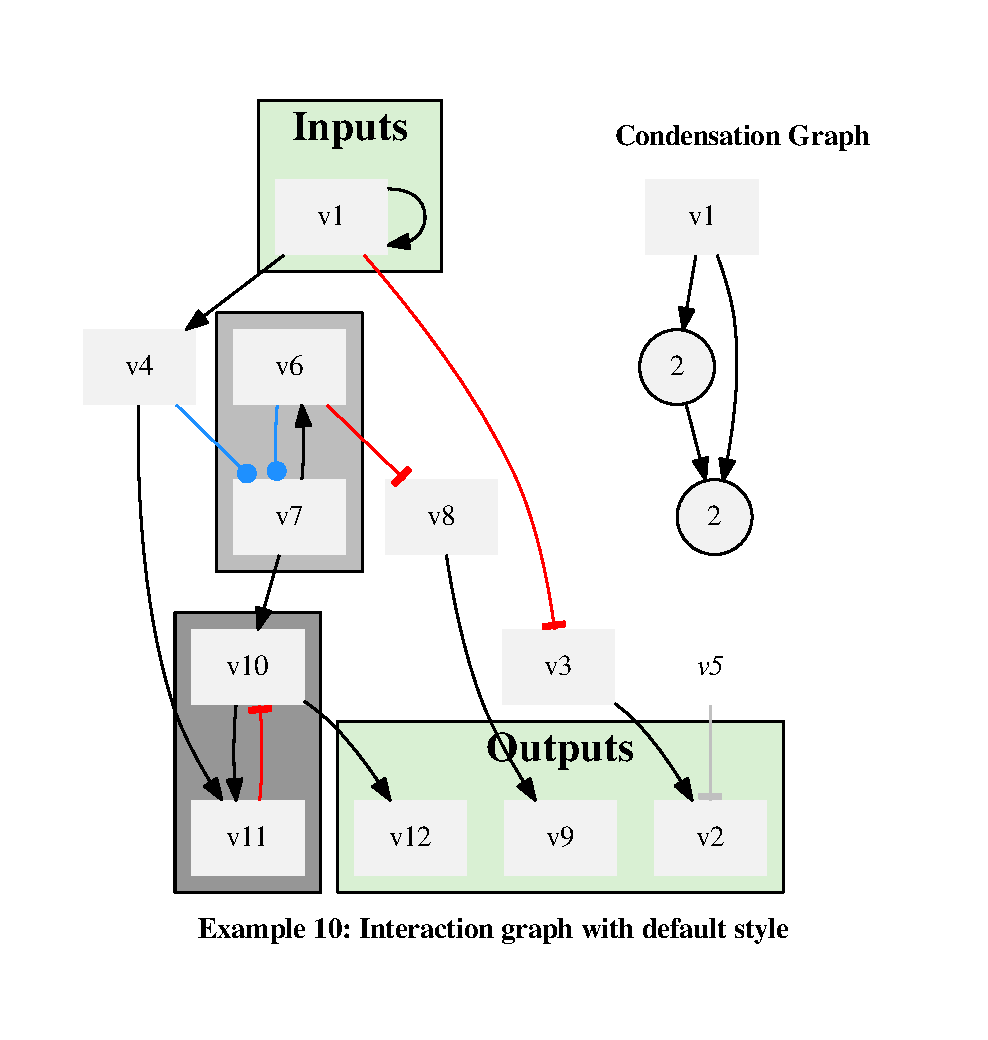
\includegraphics{figure09.pdf}}
\caption{The interaction graph ``\emph{example10\_igraph.pdf}'' with attributes added by {\hyperref[StateTransitionGraphs:add-style-default]{\emph{add\_style\_default}}}.}\label{Manual:figure09}\end{figure}


\section{Drawing the State Transition Graph}
\label{Manual:drawing-the-state-transition-graph}
Prime implicants can be used to derive the \emph{state transition graph} (STG) of a network.
To compute it, use the function {\hyperref[StateTransitionGraphs:primes2stg]{\emph{primes2stg}}} of the module {\hyperref[StateTransitionGraphs:statetransitiongraphs]{\emph{StateTransitionGraphs}}}.
It returns an instance of the {\hyperref[Installation:installation-networkx]{\emph{NetworkX}}} digraph class:

\begin{Verbatim}[commandchars=\\\{\}]
\PYG{g+gp}{\PYGZgt{}\PYGZgt{}\PYGZgt{} }\PYG{k+kn}{from} \PYG{n+nn}{PyBoolNet} \PYG{k+kn}{import} \PYG{n}{StateTransitionGraphs} \PYG{k}{as} \PYG{n}{STGs}
\PYG{g+gp}{\PYGZgt{}\PYGZgt{}\PYGZgt{} }\PYG{n}{bnet} \PYG{o}{=} \PYG{l+s}{\PYGZdq{}}\PYG{l+s+se}{\PYGZbs{}n}\PYG{l+s}{\PYGZdq{}}\PYG{o}{.}\PYG{n}{join}\PYG{p}{(}\PYG{p}{[}\PYG{l+s}{\PYGZdq{}}\PYG{l+s}{v1, v3}\PYG{l+s}{\PYGZdq{}}\PYG{p}{,}\PYG{l+s}{\PYGZdq{}}\PYG{l+s}{v2, v1}\PYG{l+s}{\PYGZdq{}}\PYG{p}{,} \PYG{l+s}{\PYGZdq{}}\PYG{l+s}{v3, v2}\PYG{l+s}{\PYGZdq{}}\PYG{p}{]}\PYG{p}{)}
\PYG{g+gp}{\PYGZgt{}\PYGZgt{}\PYGZgt{} }\PYG{n}{primes} \PYG{o}{=} \PYG{n}{FEX}\PYG{o}{.}\PYG{n}{bnet2primes}\PYG{p}{(}\PYG{n}{bnet}\PYG{p}{)}
\PYG{g+gp}{\PYGZgt{}\PYGZgt{}\PYGZgt{} }\PYG{n}{update} \PYG{o}{=} \PYG{l+s}{\PYGZdq{}}\PYG{l+s}{asynchronous}\PYG{l+s}{\PYGZdq{}}
\PYG{g+gp}{\PYGZgt{}\PYGZgt{}\PYGZgt{} }\PYG{n}{stg} \PYG{o}{=} \PYG{n}{STGs}\PYG{o}{.}\PYG{n}{primes2stg}\PYG{p}{(}\PYG{n}{primes}\PYG{p}{,} \PYG{n}{update}\PYG{p}{)}
\PYG{g+gp}{\PYGZgt{}\PYGZgt{}\PYGZgt{} }\PYG{n}{stg}
\PYG{g+go}{\PYGZlt{}networkx.classes.digraph.DiGraph object at 0xb3c7d64c\PYGZgt{}}
\end{Verbatim}

The second argument to {\hyperref[StateTransitionGraphs:primes2stg]{\emph{primes2stg}}} is either \emph{``synchronous''} or \emph{``asynchronous''} for the fully synchronous or the fully asynchronous transition relation, see e.g. {\hyperref[Bibliography:klarner2015approx]{\emph{Klarner2015(b)}}} for a formal definition.
The nodes of an STG are string representations of states, e.g. \emph{``110''}, see {\hyperref[Manual:states-subspaces-paths]{\emph{states, subspaces and paths}}}.
You may use {\hyperref[StateTransitionGraphs:state2str]{\emph{state2str}}} to convert a state dictionary into a state string.
They are vectors of activities, sorted by component names:

\begin{Verbatim}[commandchars=\\\{\}]
\PYG{g+gp}{\PYGZgt{}\PYGZgt{}\PYGZgt{} }\PYG{n}{stg}\PYG{o}{.}\PYG{n}{nodes}\PYG{p}{(}\PYG{p}{)}\PYG{p}{[}\PYG{l+m+mi}{0}\PYG{p}{]}
\PYG{g+go}{\PYGZsq{}010\PYGZsq{}}
\end{Verbatim}

You may use {\hyperref[Installation:installation-networkx]{\emph{NetworkX}}} functions on \emph{stg}, for example \href{https://networkx.github.io/documentation/latest/reference/generated/networkx.algorithms.shortest\_paths.generic.has\_path.html}{networkx.has\_path}:

\begin{Verbatim}[commandchars=\\\{\}]
\PYG{g+gp}{\PYGZgt{}\PYGZgt{}\PYGZgt{} }\PYG{k+kn}{import} \PYG{n+nn}{networkx}
\PYG{g+gp}{\PYGZgt{}\PYGZgt{}\PYGZgt{} }\PYG{n}{networkx}\PYG{o}{.}\PYG{n}{has\PYGZus{}path}\PYG{p}{(}\PYG{n}{stg}\PYG{p}{,} \PYG{l+s}{\PYGZdq{}}\PYG{l+s}{100}\PYG{l+s}{\PYGZdq{}}\PYG{p}{,} \PYG{l+s}{\PYGZdq{}}\PYG{l+s}{111}\PYG{l+s}{\PYGZdq{}}\PYG{p}{)}
\PYG{g+go}{True}
\end{Verbatim}

State transition graphs can be styled in the same way as interaction graphs, see {\hyperref[Manual:drawing-interaction-graphs]{\emph{Drawing the Interaction Graph}}}.
Use the function {\hyperref[StateTransitionGraphs:stg2image]{\emph{stg2image}}} to generate a drawing of the STG:

\begin{Verbatim}[commandchars=\\\{\}]
\PYG{g+gp}{\PYGZgt{}\PYGZgt{}\PYGZgt{} }\PYG{n}{stg}\PYG{o}{.}\PYG{n}{graph}\PYG{p}{[}\PYG{l+s}{\PYGZdq{}}\PYG{l+s}{label}\PYG{l+s}{\PYGZdq{}}\PYG{p}{]} \PYG{o}{=} \PYG{l+s}{\PYGZdq{}}\PYG{l+s}{Example 11: The asynchronous STG of a positive circuit}\PYG{l+s}{\PYGZdq{}}
\PYG{g+gp}{\PYGZgt{}\PYGZgt{}\PYGZgt{} }\PYG{n}{stg}\PYG{o}{.}\PYG{n}{graph}\PYG{p}{[}\PYG{l+s}{\PYGZdq{}}\PYG{l+s}{rankdir}\PYG{l+s}{\PYGZdq{}}\PYG{p}{]} \PYG{o}{=} \PYG{l+s}{\PYGZdq{}}\PYG{l+s}{LR}\PYG{l+s}{\PYGZdq{}}
\PYG{g+gp}{\PYGZgt{}\PYGZgt{}\PYGZgt{} }\PYG{n}{STGs}\PYG{o}{.}\PYG{n}{stg2image}\PYG{p}{(}\PYG{n}{stg}\PYG{p}{,} \PYG{l+s}{\PYGZdq{}}\PYG{l+s}{example11\PYGZus{}stg.pdf}\PYG{l+s}{\PYGZdq{}}\PYG{p}{)}
\end{Verbatim}

The result is shown in {\hyperref[Manual:figure10]{\emph{the figure below}}}.
\begin{figure}[htbp]
\centering
\capstart

\scalebox{0.800000}{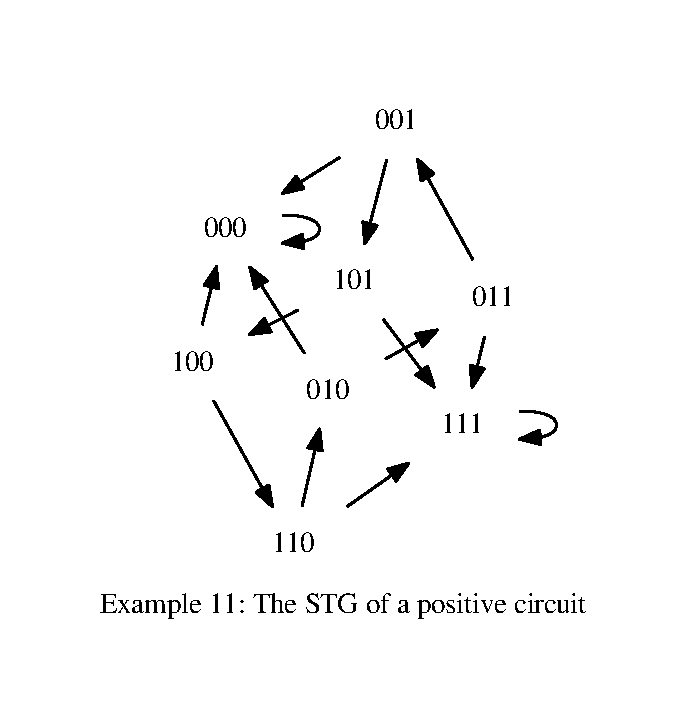
\includegraphics{figure10.pdf}}
\caption{The state transition graph ``\emph{example11\_stg.pdf}'' of an isolated feedback circuit.}\label{Manual:figure10}\end{figure}

By default, the full STG is constructed.
If you want to draw the part of a STG that is reachable from an initial state or a set of initial states
pass a third argument to {\hyperref[StateTransitionGraphs:primes2stg]{\emph{primes2stg}}}.
For convenience you may choose one of several ways of specifying initial states.
Either a list of states in \emph{dict} or \emph{str} format, see {\hyperref[Manual:states-subspaces-paths]{\emph{states, subspaces and paths}}}:

\begin{Verbatim}[commandchars=\\\{\}]
\PYG{g+gp}{\PYGZgt{}\PYGZgt{}\PYGZgt{} }\PYG{n}{init} \PYG{o}{=} \PYG{p}{[}\PYG{l+s}{\PYGZdq{}}\PYG{l+s}{000}\PYG{l+s}{\PYGZdq{}}\PYG{p}{,} \PYG{l+s}{\PYGZdq{}}\PYG{l+s}{111}\PYG{l+s}{\PYGZdq{}}\PYG{p}{]}
\PYG{g+gp}{\PYGZgt{}\PYGZgt{}\PYGZgt{} }\PYG{n}{init} \PYG{o}{=} \PYG{p}{[}\PYG{l+s}{\PYGZdq{}}\PYG{l+s}{000}\PYG{l+s}{\PYGZdq{}}\PYG{p}{,} \PYG{p}{\PYGZob{}}\PYG{l+s}{\PYGZdq{}}\PYG{l+s}{v1}\PYG{l+s}{\PYGZdq{}}\PYG{p}{:}\PYG{l+m+mi}{1}\PYG{p}{,}\PYG{l+s}{\PYGZdq{}}\PYG{l+s}{v2}\PYG{l+s}{\PYGZdq{}}\PYG{p}{:}\PYG{l+m+mi}{1}\PYG{p}{,}\PYG{l+s}{\PYGZdq{}}\PYG{l+s}{v3}\PYG{l+s}{\PYGZdq{}}\PYG{p}{:}\PYG{l+m+mi}{1}\PYG{p}{\PYGZcb{}}\PYG{p}{]}
\end{Verbatim}

or as a function that is called on every state and must return either \emph{True} or \emph{False} to indicate whether the state ought to be initial:

\begin{Verbatim}[commandchars=\\\{\}]
\PYG{g+gp}{\PYGZgt{}\PYGZgt{}\PYGZgt{} }\PYG{n}{init} \PYG{o}{=} \PYG{k}{lambda} \PYG{n}{x}\PYG{p}{:} \PYG{n}{x}\PYG{p}{[}\PYG{l+s}{\PYGZdq{}}\PYG{l+s}{v1}\PYG{l+s}{\PYGZdq{}}\PYG{p}{]}\PYG{o}{\PYGZgt{}}\PYG{o}{=}\PYG{n}{x}\PYG{p}{[}\PYG{l+s}{\PYGZdq{}}\PYG{l+s}{v2}\PYG{l+s}{\PYGZdq{}}\PYG{p}{]}
\end{Verbatim}

or by a subspace in which case all the states contained in it are initial:

\begin{Verbatim}[commandchars=\\\{\}]
\PYG{g+gp}{\PYGZgt{}\PYGZgt{}\PYGZgt{} }\PYG{n}{init} \PYG{o}{=} \PYG{l+s}{\PYGZdq{}}\PYG{l+s}{\PYGZhy{}\PYGZhy{}1}\PYG{l+s}{\PYGZdq{}}
\PYG{g+gp}{\PYGZgt{}\PYGZgt{}\PYGZgt{} }\PYG{n}{init} \PYG{o}{=} \PYG{p}{\PYGZob{}}\PYG{l+s}{\PYGZdq{}}\PYG{l+s}{v3}\PYG{l+s}{\PYGZdq{}}\PYG{p}{:}\PYG{l+m+mi}{1}\PYG{p}{\PYGZcb{}}
\end{Verbatim}

To construct the STG starting from initial states call:

\begin{Verbatim}[commandchars=\\\{\}]
\PYG{g+gp}{\PYGZgt{}\PYGZgt{}\PYGZgt{} }\PYG{n}{stg} \PYG{o}{=} \PYG{n}{STGs}\PYG{o}{.}\PYG{n}{primes2stg}\PYG{p}{(}\PYG{n}{primes}\PYG{p}{,} \PYG{n}{update}\PYG{p}{,} \PYG{n}{init}\PYG{p}{)}
\end{Verbatim}

\begin{notice}{warning}{Warning:}
You should not draw asynchronous STGs with more than 2\textasciicircum{}7=128 states as \emph{dot} will take very long to compute the layout.
For synchronous STGs you should not go above 2\textasciicircum{}12=4096 states.
Use different layout engines like \emph{twopi} and \emph{circo} by generating the \emph{dot} file with {\hyperref[StateTransitionGraphs:stg2dot]{\emph{stg2dot}}} and compiling it manually.
\end{notice}


\subsection{the tendencies style}
\label{Manual:the-tendencies-style}
The tendencies style for state transition graphs is similar to the interaction sign style for interaction graphs.
It colors state transitions according to whether all changing variables increase (black), or all of them decrease (red) or some increase and some decrease (blue).
The latter is only possible for synchronous transition graphs.

Here is an example:

\begin{Verbatim}[commandchars=\\\{\}]
\PYG{g+gp}{\PYGZgt{}\PYGZgt{}\PYGZgt{} }\PYG{n}{bnet} \PYG{o}{=} \PYG{l+s}{\PYGZdq{}}\PYG{l+s+se}{\PYGZbs{}n}\PYG{l+s}{\PYGZdq{}}\PYG{o}{.}\PYG{n}{join}\PYG{p}{(}\PYG{p}{[}\PYG{l+s}{\PYGZdq{}}\PYG{l+s}{v1, !v3}\PYG{l+s}{\PYGZdq{}}\PYG{p}{,}\PYG{l+s}{\PYGZdq{}}\PYG{l+s}{v2, v1}\PYG{l+s}{\PYGZdq{}}\PYG{p}{,} \PYG{l+s}{\PYGZdq{}}\PYG{l+s}{v3, v2}\PYG{l+s}{\PYGZdq{}}\PYG{p}{]}\PYG{p}{)}
\PYG{g+gp}{\PYGZgt{}\PYGZgt{}\PYGZgt{} }\PYG{n}{primes} \PYG{o}{=} \PYG{n}{FEX}\PYG{o}{.}\PYG{n}{bnet2primes}\PYG{p}{(}\PYG{n}{bnet}\PYG{p}{)}
\PYG{g+gp}{\PYGZgt{}\PYGZgt{}\PYGZgt{} }\PYG{n}{stg} \PYG{o}{=} \PYG{n}{STGs}\PYG{o}{.}\PYG{n}{primes2stg}\PYG{p}{(}\PYG{n}{primes}\PYG{p}{,} \PYG{l+s}{\PYGZdq{}}\PYG{l+s}{synchronous}\PYG{l+s}{\PYGZdq{}}\PYG{p}{)}
\PYG{g+gp}{\PYGZgt{}\PYGZgt{}\PYGZgt{} }\PYG{n}{stg}\PYG{o}{.}\PYG{n}{graph}\PYG{p}{[}\PYG{l+s}{\PYGZdq{}}\PYG{l+s}{rankdir}\PYG{l+s}{\PYGZdq{}}\PYG{p}{]} \PYG{o}{=} \PYG{l+s}{\PYGZdq{}}\PYG{l+s}{LR}\PYG{l+s}{\PYGZdq{}}
\PYG{g+gp}{\PYGZgt{}\PYGZgt{}\PYGZgt{} }\PYG{n}{stg}\PYG{o}{.}\PYG{n}{graph}\PYG{p}{[}\PYG{l+s}{\PYGZdq{}}\PYG{l+s}{label}\PYG{l+s}{\PYGZdq{}}\PYG{p}{]} \PYG{o}{=} \PYG{l+s}{\PYGZdq{}}\PYG{l+s}{Example 12: The synchronous STG of a negative circuit}\PYG{l+s}{\PYGZdq{}}
\PYG{g+gp}{\PYGZgt{}\PYGZgt{}\PYGZgt{} }\PYG{n}{STGs}\PYG{o}{.}\PYG{n}{add\PYGZus{}style\PYGZus{}tendencies}\PYG{p}{(}\PYG{n}{stg}\PYG{p}{)}
\PYG{g+gp}{\PYGZgt{}\PYGZgt{}\PYGZgt{} }\PYG{n}{STGs}\PYG{o}{.}\PYG{n}{stg2image}\PYG{p}{(}\PYG{n}{stg}\PYG{p}{,} \PYG{l+s}{\PYGZdq{}}\PYG{l+s}{example12\PYGZus{}stg.pdf}\PYG{l+s}{\PYGZdq{}}\PYG{p}{)}
\end{Verbatim}

The result is shown in {\hyperref[Manual:figure11]{\emph{the figure below}}}.
\begin{figure}[htbp]
\centering
\capstart

\scalebox{0.800000}{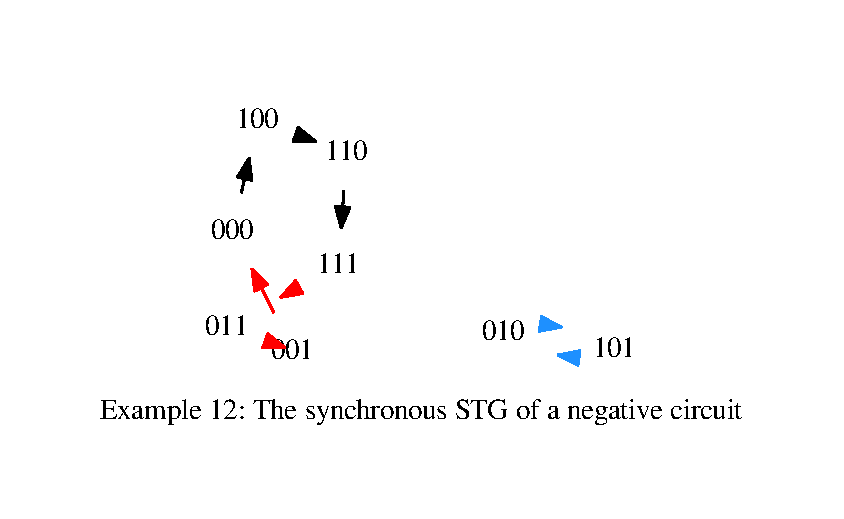
\includegraphics{figure11.pdf}}
\caption{The state transition graph ``\emph{example12\_stg.pdf}'' with attributes added by {\hyperref[StateTransitionGraphs:add-style-tendencies]{\emph{add\_style\_tendencies}}}.}\label{Manual:figure11}\end{figure}


\subsection{the path style}
\label{Manual:the-path-style}
The path style is used to highlight a path in the state transition graph.
It changes the \emph{penwidth} and \emph{color} of transitions.

Consider the following example:

\begin{Verbatim}[commandchars=\\\{\}]
\PYG{g+gp}{\PYGZgt{}\PYGZgt{}\PYGZgt{} }\PYG{n}{bnet} \PYG{o}{=} \PYG{l+s}{\PYGZdq{}}\PYG{l+s+se}{\PYGZbs{}n}\PYG{l+s}{\PYGZdq{}}\PYG{o}{.}\PYG{n}{join}\PYG{p}{(}\PYG{p}{[}\PYG{l+s}{\PYGZdq{}}\PYG{l+s}{x, !x\textbar{}y}\PYG{l+s}{\PYGZdq{}}\PYG{p}{,} \PYG{l+s}{\PYGZdq{}}\PYG{l+s}{y, !x\PYGZam{}!z\textbar{}x\PYGZam{}!y\PYGZam{}z}\PYG{l+s}{\PYGZdq{}}\PYG{p}{,} \PYG{l+s}{\PYGZdq{}}\PYG{l+s}{z, x\textbar{}!y}\PYG{l+s}{\PYGZdq{}}\PYG{p}{]}\PYG{p}{)}
\PYG{g+gp}{\PYGZgt{}\PYGZgt{}\PYGZgt{} }\PYG{n}{primes} \PYG{o}{=} \PYG{n}{FEX}\PYG{o}{.}\PYG{n}{bnet2primes}\PYG{p}{(}\PYG{n}{bnet}\PYG{p}{)}
\PYG{g+gp}{\PYGZgt{}\PYGZgt{}\PYGZgt{} }\PYG{n}{stg} \PYG{o}{=} \PYG{n}{STGs}\PYG{o}{.}\PYG{n}{primes2stg}\PYG{p}{(}\PYG{n}{primes}\PYG{p}{,} \PYG{l+s}{\PYGZdq{}}\PYG{l+s}{asynchronous}\PYG{l+s}{\PYGZdq{}}\PYG{p}{)}
\PYG{g+gp}{\PYGZgt{}\PYGZgt{}\PYGZgt{} }\PYG{n}{stg}\PYG{o}{.}\PYG{n}{graph}\PYG{p}{[}\PYG{l+s}{\PYGZdq{}}\PYG{l+s}{label}\PYG{l+s}{\PYGZdq{}}\PYG{p}{]} \PYG{o}{=} \PYG{l+s}{\PYGZdq{}}\PYG{l+s}{Example 13: STG with path style}\PYG{l+s}{\PYGZdq{}}
\end{Verbatim}

Now add the path style:

\begin{Verbatim}[commandchars=\\\{\}]
\PYG{g+gp}{\PYGZgt{}\PYGZgt{}\PYGZgt{} }\PYG{n}{path} \PYG{o}{=} \PYG{p}{[}\PYG{l+s}{\PYGZdq{}}\PYG{l+s}{011}\PYG{l+s}{\PYGZdq{}}\PYG{p}{,}\PYG{l+s}{\PYGZdq{}}\PYG{l+s}{010}\PYG{l+s}{\PYGZdq{}}\PYG{p}{,}\PYG{l+s}{\PYGZdq{}}\PYG{l+s}{110}\PYG{l+s}{\PYGZdq{}}\PYG{p}{,}\PYG{l+s}{\PYGZdq{}}\PYG{l+s}{100}\PYG{l+s}{\PYGZdq{}}\PYG{p}{,}\PYG{l+s}{\PYGZdq{}}\PYG{l+s}{000}\PYG{l+s}{\PYGZdq{}}\PYG{p}{]}
\PYG{g+gp}{\PYGZgt{}\PYGZgt{}\PYGZgt{} }\PYG{n}{STGs}\PYG{o}{.}\PYG{n}{add\PYGZus{}style\PYGZus{}path}\PYG{p}{(}\PYG{n}{stg}\PYG{p}{,} \PYG{n}{path}\PYG{p}{,} \PYG{l+s}{\PYGZdq{}}\PYG{l+s}{red}\PYG{l+s}{\PYGZdq{}}\PYG{p}{)}
\PYG{g+gp}{\PYGZgt{}\PYGZgt{}\PYGZgt{} }\PYG{n}{STGs}\PYG{o}{.}\PYG{n}{stg2image}\PYG{p}{(}\PYG{n}{stg}\PYG{p}{,} \PYG{l+s}{\PYGZdq{}}\PYG{l+s}{example13\PYGZus{}stg.pdf}\PYG{l+s}{\PYGZdq{}}\PYG{p}{)}
\end{Verbatim}

The result is shown in {\hyperref[Manual:figure12]{\emph{the figure below}}}.
\begin{figure}[htbp]
\centering
\capstart

\scalebox{0.600000}{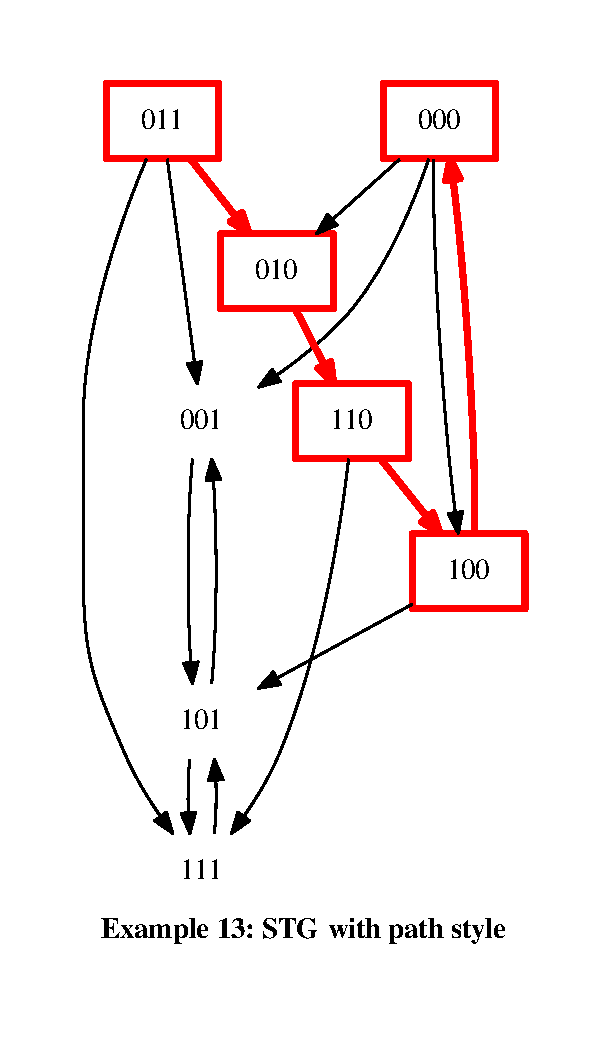
\includegraphics{figure12.pdf}}
\caption{The state transition graph ``\emph{example13\_stg.pdf}'' with attributes added by {\hyperref[StateTransitionGraphs:add-style-path]{\emph{add\_style\_path}}}.}\label{Manual:figure12}\end{figure}


\subsection{the SCCs style}
\label{Manual:id4}
The SCC style is almost identical to the one for interaction graphs except that it adds a label to the attractors, i.e.,
steady states and cyclic attractors.:

\begin{Verbatim}[commandchars=\\\{\}]
\PYG{g+gp}{\PYGZgt{}\PYGZgt{}\PYGZgt{} }\PYG{n}{bnet} \PYG{o}{=} \PYG{l+s}{\PYGZdq{}}\PYG{l+s+se}{\PYGZbs{}n}\PYG{l+s}{\PYGZdq{}}\PYG{o}{.}\PYG{n}{join}\PYG{p}{(}\PYG{p}{[}\PYG{l+s}{\PYGZdq{}}\PYG{l+s}{x, !x\textbar{}y}\PYG{l+s}{\PYGZdq{}}\PYG{p}{,} \PYG{l+s}{\PYGZdq{}}\PYG{l+s}{y, x\PYGZam{}!y\textbar{}!z}\PYG{l+s}{\PYGZdq{}}\PYG{p}{,} \PYG{l+s}{\PYGZdq{}}\PYG{l+s}{z, x\PYGZam{}z\textbar{}!y}\PYG{l+s}{\PYGZdq{}}\PYG{p}{]}\PYG{p}{)}
\PYG{g+gp}{\PYGZgt{}\PYGZgt{}\PYGZgt{} }\PYG{n}{primes} \PYG{o}{=} \PYG{n}{FEX}\PYG{o}{.}\PYG{n}{bnet2primes}\PYG{p}{(}\PYG{n}{bnet}\PYG{p}{)}
\PYG{g+gp}{\PYGZgt{}\PYGZgt{}\PYGZgt{} }\PYG{n}{stg} \PYG{o}{=} \PYG{n}{STGs}\PYG{o}{.}\PYG{n}{primes2stg}\PYG{p}{(}\PYG{n}{primes}\PYG{p}{,} \PYG{l+s}{\PYGZdq{}}\PYG{l+s}{asynchronous}\PYG{l+s}{\PYGZdq{}}\PYG{p}{)}
\PYG{g+gp}{\PYGZgt{}\PYGZgt{}\PYGZgt{} }\PYG{n}{stg}\PYG{o}{.}\PYG{n}{graph}\PYG{p}{[}\PYG{l+s}{\PYGZdq{}}\PYG{l+s}{label}\PYG{l+s}{\PYGZdq{}}\PYG{p}{]} \PYG{o}{=} \PYG{l+s}{\PYGZdq{}}\PYG{l+s}{The SCC style}\PYG{l+s}{\PYGZdq{}}
\PYG{g+gp}{\PYGZgt{}\PYGZgt{}\PYGZgt{} }\PYG{n}{STGs}\PYG{o}{.}\PYG{n}{add\PYGZus{}style\PYGZus{}sccs}\PYG{p}{(}\PYG{n}{stg}\PYG{p}{)}
\PYG{g+gp}{\PYGZgt{}\PYGZgt{}\PYGZgt{} }\PYG{n}{STGs}\PYG{o}{.}\PYG{n}{stg2image}\PYG{p}{(}\PYG{n}{stg}\PYG{p}{,} \PYG{l+s}{\PYGZdq{}}\PYG{l+s}{example14\PYGZus{}stg.pdf}\PYG{l+s}{\PYGZdq{}}\PYG{p}{)}
\end{Verbatim}

The result is shown in {\hyperref[Manual:figure13]{\emph{the figure below}}}.
\begin{figure}[htbp]
\centering
\capstart

\scalebox{0.600000}{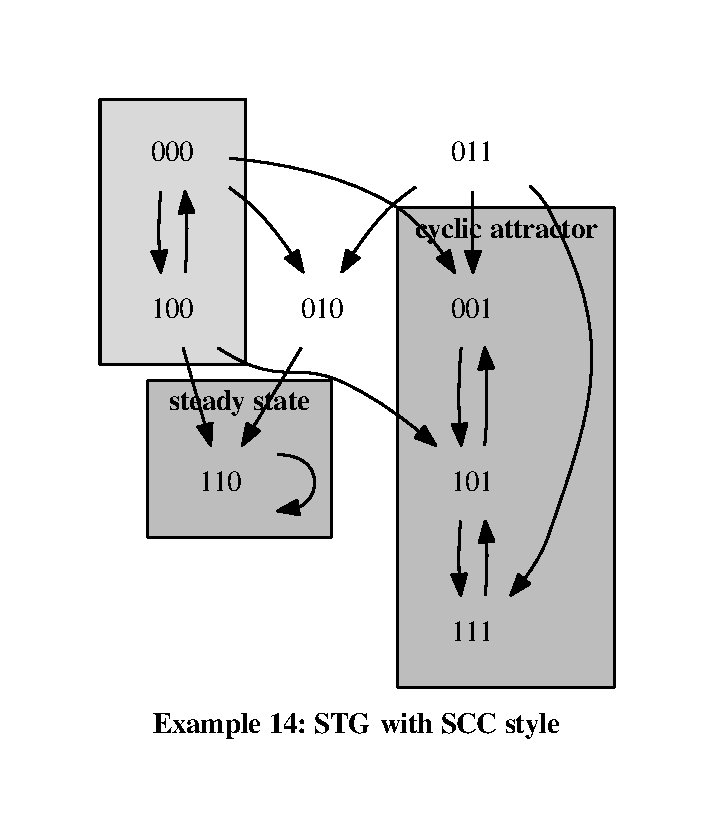
\includegraphics{figure13.pdf}}
\caption{The state transition graph ``\emph{example14\_stg.pdf}'' with attributes added by {\hyperref[StateTransitionGraphs:add-style-sccs]{\emph{add\_style\_sccs}}}.}\label{Manual:figure13}\end{figure}


\subsection{the min trap spaces style}
\label{Manual:the-min-trap-spaces-style}
The min trap spaces style is adds a \emph{dot} subgraph for every minimal trap space of the state transition graph.
For an introduction to trap spaces, see {\hyperref[Bibliography:klarner2015trap]{\emph{Klarner2015(a)}}} and also \emph{trap\_spaces\_and\_attractors}:

\begin{Verbatim}[commandchars=\\\{\}]
\PYG{g+gp}{\PYGZgt{}\PYGZgt{}\PYGZgt{} }\PYG{n}{bnet} \PYG{o}{=} \PYG{l+s}{\PYGZdq{}}\PYG{l+s+se}{\PYGZbs{}n}\PYG{l+s}{\PYGZdq{}}\PYG{o}{.}\PYG{n}{join}\PYG{p}{(}\PYG{p}{[}\PYG{l+s}{\PYGZdq{}}\PYG{l+s}{x, !x\textbar{}y\PYGZam{}z}\PYG{l+s}{\PYGZdq{}}\PYG{p}{,} \PYG{l+s}{\PYGZdq{}}\PYG{l+s}{y, x\PYGZam{}!y\textbar{}!z}\PYG{l+s}{\PYGZdq{}}\PYG{p}{,} \PYG{l+s}{\PYGZdq{}}\PYG{l+s}{z, z\textbar{}!y}\PYG{l+s}{\PYGZdq{}}\PYG{p}{]}\PYG{p}{)}
\PYG{g+gp}{\PYGZgt{}\PYGZgt{}\PYGZgt{} }\PYG{n}{primes} \PYG{o}{=} \PYG{n}{FEX}\PYG{o}{.}\PYG{n}{bnet2primes}\PYG{p}{(}\PYG{n}{bnet}\PYG{p}{)}
\PYG{g+gp}{\PYGZgt{}\PYGZgt{}\PYGZgt{} }\PYG{n}{stg} \PYG{o}{=} \PYG{n}{STGs}\PYG{o}{.}\PYG{n}{primes2stg}\PYG{p}{(}\PYG{n}{primes}\PYG{p}{,} \PYG{l+s}{\PYGZdq{}}\PYG{l+s}{asynchronous}\PYG{l+s}{\PYGZdq{}}\PYG{p}{)}
\PYG{g+gp}{\PYGZgt{}\PYGZgt{}\PYGZgt{} }\PYG{n}{stg}\PYG{o}{.}\PYG{n}{graph}\PYG{p}{[}\PYG{l+s}{\PYGZdq{}}\PYG{l+s}{label}\PYG{l+s}{\PYGZdq{}}\PYG{p}{]} \PYG{o}{=} \PYG{l+s}{\PYGZdq{}}\PYG{l+s}{Example 15: STG with min trap spaces style}\PYG{l+s}{\PYGZdq{}}
\PYG{g+gp}{\PYGZgt{}\PYGZgt{}\PYGZgt{} }\PYG{n}{STGs}\PYG{o}{.}\PYG{n}{add\PYGZus{}style\PYGZus{}mintrapspaces}\PYG{p}{(}\PYG{n}{primes}\PYG{p}{,} \PYG{n}{stg}\PYG{p}{)}
\PYG{g+gp}{\PYGZgt{}\PYGZgt{}\PYGZgt{} }\PYG{n}{STGs}\PYG{o}{.}\PYG{n}{stg2image}\PYG{p}{(}\PYG{n}{stg}\PYG{p}{,} \PYG{l+s}{\PYGZdq{}}\PYG{l+s}{example15\PYGZus{}stg.pdf}\PYG{l+s}{\PYGZdq{}}\PYG{p}{)}
\end{Verbatim}

The result is shown in {\hyperref[Manual:figure14]{\emph{the figure below}}}.
\begin{figure}[htbp]
\centering
\capstart

\scalebox{0.600000}{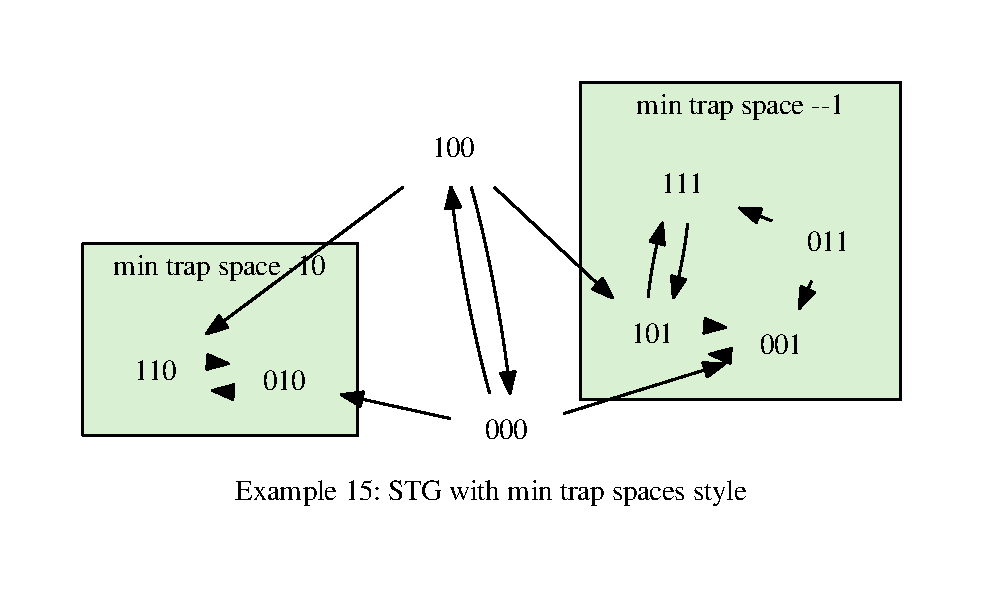
\includegraphics{figure14.pdf}}
\caption{The state transition graph ``\emph{example15\_stg.pdf}'' with attributes added by {\hyperref[StateTransitionGraphs:add-style-mintrapspaces]{\emph{add\_style\_mintrapspaces}}}.}\label{Manual:figure14}\end{figure}


\subsection{the subspaces style}
\label{Manual:the-subspaces-style}
The subspace style is identical to the subgraph style of interaction graphs.
It adds a subgraph for every given subspace.
As for interaction graphs, you may add pairs of subspace and attribute dictionaries if you want to change the label, or color etc. of the subgraphs:

\begin{Verbatim}[commandchars=\\\{\}]
\PYG{g+gp}{\PYGZgt{}\PYGZgt{}\PYGZgt{} }\PYG{n}{bnet} \PYG{o}{=} \PYG{l+s}{\PYGZdq{}}\PYG{l+s+se}{\PYGZbs{}n}\PYG{l+s}{\PYGZdq{}}\PYG{o}{.}\PYG{n}{join}\PYG{p}{(}\PYG{p}{[}\PYG{l+s}{\PYGZdq{}}\PYG{l+s}{x, !x\textbar{}y\PYGZam{}z}\PYG{l+s}{\PYGZdq{}}\PYG{p}{,} \PYG{l+s}{\PYGZdq{}}\PYG{l+s}{y, x\PYGZam{}!y\textbar{}!z}\PYG{l+s}{\PYGZdq{}}\PYG{p}{,} \PYG{l+s}{\PYGZdq{}}\PYG{l+s}{z, z\textbar{}!y}\PYG{l+s}{\PYGZdq{}}\PYG{p}{]}\PYG{p}{)}
\PYG{g+gp}{\PYGZgt{}\PYGZgt{}\PYGZgt{} }\PYG{n}{primes} \PYG{o}{=} \PYG{n}{FEX}\PYG{o}{.}\PYG{n}{bnet2primes}\PYG{p}{(}\PYG{n}{bnet}\PYG{p}{)}
\PYG{g+gp}{\PYGZgt{}\PYGZgt{}\PYGZgt{} }\PYG{n}{stg} \PYG{o}{=} \PYG{n}{STGs}\PYG{o}{.}\PYG{n}{primes2stg}\PYG{p}{(}\PYG{n}{primes}\PYG{p}{,} \PYG{l+s}{\PYGZdq{}}\PYG{l+s}{asynchronous}\PYG{l+s}{\PYGZdq{}}\PYG{p}{)}
\PYG{g+gp}{\PYGZgt{}\PYGZgt{}\PYGZgt{} }\PYG{n}{stg}\PYG{o}{.}\PYG{n}{graph}\PYG{p}{[}\PYG{l+s}{\PYGZdq{}}\PYG{l+s}{label}\PYG{l+s}{\PYGZdq{}}\PYG{p}{]} \PYG{o}{=} \PYG{l+s}{\PYGZdq{}}\PYG{l+s}{Example 16: STG with subspaces style}\PYG{l+s}{\PYGZdq{}}
\PYG{g+gp}{\PYGZgt{}\PYGZgt{}\PYGZgt{} }\PYG{n}{sub1} \PYG{o}{=} \PYG{p}{(}\PYG{p}{\PYGZob{}}\PYG{l+s}{\PYGZdq{}}\PYG{l+s}{x}\PYG{l+s}{\PYGZdq{}}\PYG{p}{:}\PYG{l+m+mi}{0}\PYG{p}{\PYGZcb{}}\PYG{p}{,}\PYG{p}{\PYGZob{}}\PYG{l+s}{\PYGZdq{}}\PYG{l+s}{label}\PYG{l+s}{\PYGZdq{}}\PYG{p}{:}\PYG{l+s}{\PYGZdq{}}\PYG{l+s}{x is zero}\PYG{l+s}{\PYGZdq{}}\PYG{p}{\PYGZcb{}}\PYG{p}{)}
\PYG{g+gp}{\PYGZgt{}\PYGZgt{}\PYGZgt{} }\PYG{n}{sub2} \PYG{o}{=} \PYG{p}{\PYGZob{}}\PYG{l+s}{\PYGZdq{}}\PYG{l+s}{x}\PYG{l+s}{\PYGZdq{}}\PYG{p}{:}\PYG{l+m+mi}{1}\PYG{p}{,}\PYG{l+s}{\PYGZdq{}}\PYG{l+s}{y}\PYG{l+s}{\PYGZdq{}}\PYG{p}{:}\PYG{l+m+mi}{0}\PYG{p}{\PYGZcb{}}
\PYG{g+gp}{\PYGZgt{}\PYGZgt{}\PYGZgt{} }\PYG{n}{subspaces} \PYG{o}{=} \PYG{p}{[}\PYG{n}{sub1}\PYG{p}{,} \PYG{n}{sub2}\PYG{p}{]}
\PYG{g+gp}{\PYGZgt{}\PYGZgt{}\PYGZgt{} }\PYG{n}{STGs}\PYG{o}{.}\PYG{n}{add\PYGZus{}style\PYGZus{}subspaces}\PYG{p}{(}\PYG{n}{primes}\PYG{p}{,} \PYG{n}{stg}\PYG{p}{,} \PYG{n}{subspaces}\PYG{p}{)}
\PYG{g+gp}{\PYGZgt{}\PYGZgt{}\PYGZgt{} }\PYG{n}{STGs}\PYG{o}{.}\PYG{n}{stg2image}\PYG{p}{(}\PYG{n}{stg}\PYG{p}{,} \PYG{l+s}{\PYGZdq{}}\PYG{l+s}{example16\PYGZus{}stg.pdf}\PYG{l+s}{\PYGZdq{}}\PYG{p}{)}
\end{Verbatim}

The result is shown in {\hyperref[Manual:figure15]{\emph{the figure below}}}.

\begin{notice}{note}{Note:}
\emph{Subspaces} must satisfy this property:
Any two subspaces have either empty intersection or one is a subset of the other.
The reason for this requirement is that \emph{dot} can not draw intersecting subgraphs.
\end{notice}
\begin{figure}[htbp]
\centering
\capstart

\scalebox{0.600000}{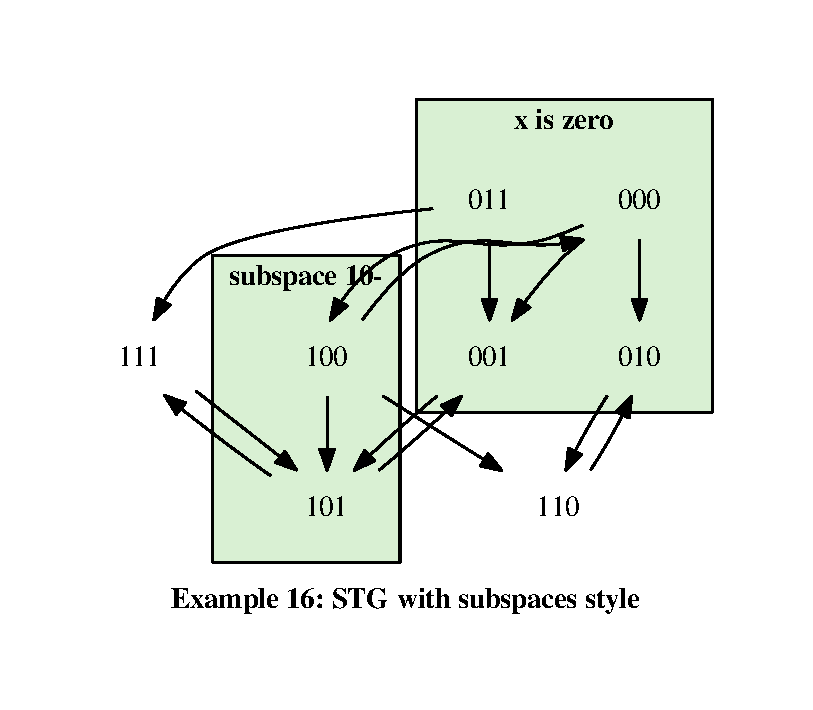
\includegraphics{figure15.pdf}}
\caption{The state transition graph \emph{``example16\_stg.pdf''} with attributes added by {\hyperref[StateTransitionGraphs:add-style-subspaces]{\emph{add\_style\_subspaces}}}.}\label{Manual:figure15}\end{figure}


\subsection{the default style}
\label{Manual:id5}
The default style combines the SCCs with the tendencies and the minimal trap spaces styles:

\begin{Verbatim}[commandchars=\\\{\}]
\PYG{g+gp}{\PYGZgt{}\PYGZgt{}\PYGZgt{} }\PYG{n}{bnet} \PYG{o}{=} \PYG{l+s}{\PYGZdq{}}\PYG{l+s+se}{\PYGZbs{}n}\PYG{l+s}{\PYGZdq{}}\PYG{o}{.}\PYG{n}{join}\PYG{p}{(}\PYG{p}{[}\PYG{l+s}{\PYGZdq{}}\PYG{l+s}{x, !x\textbar{}y\PYGZam{}z}\PYG{l+s}{\PYGZdq{}}\PYG{p}{,} \PYG{l+s}{\PYGZdq{}}\PYG{l+s}{y, x\PYGZam{}!y\textbar{}!z}\PYG{l+s}{\PYGZdq{}}\PYG{p}{,} \PYG{l+s}{\PYGZdq{}}\PYG{l+s}{z, z\textbar{}!y}\PYG{l+s}{\PYGZdq{}}\PYG{p}{]}\PYG{p}{)}
\PYG{g+gp}{\PYGZgt{}\PYGZgt{}\PYGZgt{} }\PYG{n}{primes} \PYG{o}{=} \PYG{n}{FEX}\PYG{o}{.}\PYG{n}{bnet2primes}\PYG{p}{(}\PYG{n}{bnet}\PYG{p}{)}
\PYG{g+gp}{\PYGZgt{}\PYGZgt{}\PYGZgt{} }\PYG{n}{stg} \PYG{o}{=} \PYG{n}{STGs}\PYG{o}{.}\PYG{n}{primes2stg}\PYG{p}{(}\PYG{n}{primes}\PYG{p}{,} \PYG{l+s}{\PYGZdq{}}\PYG{l+s}{asynchronous}\PYG{l+s}{\PYGZdq{}}\PYG{p}{)}
\PYG{g+gp}{\PYGZgt{}\PYGZgt{}\PYGZgt{} }\PYG{n}{stg}\PYG{o}{.}\PYG{n}{graph}\PYG{p}{[}\PYG{l+s}{\PYGZdq{}}\PYG{l+s}{label}\PYG{l+s}{\PYGZdq{}}\PYG{p}{]} \PYG{o}{=} \PYG{l+s}{\PYGZdq{}}\PYG{l+s}{Example 16: STG with default style}\PYG{l+s}{\PYGZdq{}}
\PYG{g+gp}{\PYGZgt{}\PYGZgt{}\PYGZgt{} }\PYG{n}{STGs}\PYG{o}{.}\PYG{n}{add\PYGZus{}style\PYGZus{}default}\PYG{p}{(}\PYG{n}{primes}\PYG{p}{,} \PYG{n}{stg}\PYG{p}{)}
\PYG{g+gp}{\PYGZgt{}\PYGZgt{}\PYGZgt{} }\PYG{n}{STGs}\PYG{o}{.}\PYG{n}{stg2image}\PYG{p}{(}\PYG{n}{stg}\PYG{p}{,} \PYG{l+s}{\PYGZdq{}}\PYG{l+s}{example17\PYGZus{}stg.pdf}\PYG{l+s}{\PYGZdq{}}\PYG{p}{)}
\end{Verbatim}

The result is shown in {\hyperref[Manual:figure16]{\emph{the figure below}}}.
\begin{figure}[htbp]
\centering
\capstart

\scalebox{0.800000}{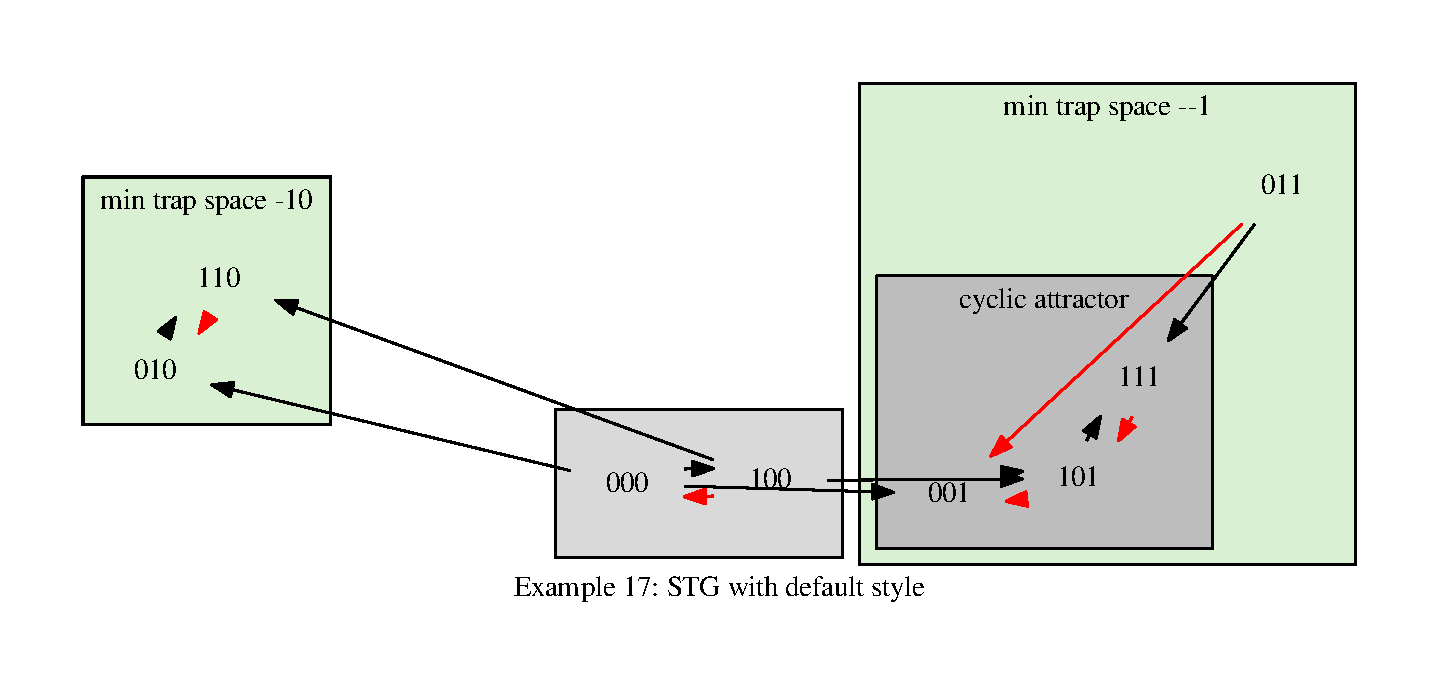
\includegraphics{figure16.pdf}}
\caption{The state transition graph \emph{``example17\_stg.pdf''} with attributes added by {\hyperref[StateTransitionGraphs:add-style-default]{\emph{add\_style\_default}}}.}\label{Manual:figure16}\end{figure}


\section{Modifying Networks}
\label{Manual:sec-modifying-networks}\label{Manual:modifying-networks}

\subsection{constant, inputs and blinkers}
\label{Manual:constant-inputs-and-blinkers}
There are various reasons why it may be required to modify an imported Boolean network, i.e., a primes dictionary.
A typical example is when the goal is to enumerate a number of variations of a given network structure in order to collect those that satisfy a given specification, i.e., a model checking query.
Functions for the modification of networks are contained in the module {\hyperref[PrimeImplicants:primeimplicants]{\emph{PrimeImplicants}}}.
Typically, these functions either find something, e.g. {\hyperref[PrimeImplicants:find-inputs]{\emph{find\_inputs}}},
or create something, e.g. {\hyperref[PrimeImplicants:create-constants]{\emph{create\_constants}}} or remove something, e.g. {\hyperref[PrimeImplicants:remove-variables]{\emph{remove\_variables}}}.
But there are also functions that percolate values, enumerate input combinations and replace update functions.

As an example consider the task of replacing all constant nodes by so-called \emph{blinkers}, i.e.,
variables that are negatively auto-regulated and are therefore repetatively changing their activity from \emph{On} to \emph{Off} back to \emph{On}, and so on.
A node v1 is constant if in the \emph{bnet} file it is defined by either 0 or 1, e.g.:

\begin{Verbatim}[commandchars=\\\{\}]
\PYG{n}{v1}\PYG{p}{,}   \PYG{l+m+mi}{0}
\end{Verbatim}

Note that such a node is not an input. A node v2 is an input iff:

\begin{Verbatim}[commandchars=\\\{\}]
\PYG{n}{v2}\PYG{p}{,}   \PYG{n}{v2}
\end{Verbatim}

The difference is also visible in the interaction graph where constants have in-degree 0 and input are only regulated by themselves and the regulation is positive.
Finally, a blinker is like an input but with negative auto-regulation, e.g. v3 is a blinker iff:

\begin{Verbatim}[commandchars=\\\{\}]
v3,   !v3
\end{Verbatim}

To replace all constants by blinker first we first need the names of the constants.
If they are not known beforehand they may be computed using the function {\hyperref[PrimeImplicants:find-constants]{\emph{find\_constants}}}.
To create the blinkers use the function {\hyperref[PrimeImplicants:create-blinkers]{\emph{create\_blinkers}}}:

\begin{Verbatim}[commandchars=\\\{\}]
\PYG{g+gp}{\PYGZgt{}\PYGZgt{}\PYGZgt{} }\PYG{k+kn}{from} \PYG{n+nn}{PyBoolNet} \PYG{k+kn}{import} \PYG{n}{PrimeImplicants} \PYG{k}{as} \PYG{n}{PIs}
\PYG{g+gp}{\PYGZgt{}\PYGZgt{}\PYGZgt{} }\PYG{n}{bnet} \PYG{o}{=} \PYG{l+s}{\PYGZdq{}\PYGZdq{}\PYGZdq{}}
\PYG{g+gp}{... }\PYG{l+s}{v1,   0}
\PYG{g+gp}{... }\PYG{l+s}{v2,   1}
\PYG{g+gp}{... }\PYG{l+s}{v3,   v1\PYGZam{}v2\PYGZam{}v3\PYGZam{}v4}
\PYG{g+gp}{... }\PYG{l+s}{v4,   v3 \PYGZam{} (v1\textbar{}v2)}\PYG{l+s}{\PYGZdq{}\PYGZdq{}\PYGZdq{}}

\PYG{g+gp}{\PYGZgt{}\PYGZgt{}\PYGZgt{} }\PYG{n}{primes} \PYG{o}{=} \PYG{n}{FEX}\PYG{o}{.}\PYG{n}{bnet2pirmes}\PYG{p}{(}\PYG{n}{bnet}\PYG{p}{)}
\PYG{g+gp}{\PYGZgt{}\PYGZgt{}\PYGZgt{} }\PYG{n}{names} \PYG{o}{=} \PYG{n}{PIs}\PYG{o}{.}\PYG{n}{find\PYGZus{}constants}\PYG{p}{(}\PYG{n}{primes}\PYG{p}{)}
\PYG{g+gp}{\PYGZgt{}\PYGZgt{}\PYGZgt{} }\PYG{n}{names}
\PYG{g+go}{[\PYGZsq{}v1\PYGZsq{},\PYGZsq{}v2\PYGZsq{}]}
\PYG{g+gp}{\PYGZgt{}\PYGZgt{}\PYGZgt{} }\PYG{n}{PIs}\PYG{o}{.}\PYG{n}{create\PYGZus{}blinkers}\PYG{p}{(}\PYG{n}{primes}\PYG{p}{,} \PYG{n}{names}\PYG{p}{)}
\PYG{g+gp}{\PYGZgt{}\PYGZgt{}\PYGZgt{} }\PYG{n}{FEX}\PYG{o}{.}\PYG{n}{primes2bnet}\PYG{p}{(}\PYG{n}{primes}\PYG{p}{)}
\PYG{g+go}{v1,   !v1}
\PYG{g+go}{v2,   !v2}
\PYG{g+go}{v3,   v1 \PYGZam{} v2 \PYGZam{} v3 \PYGZam{} v4}
\PYG{g+go}{v4,   v2 \PYGZam{} v3 \textbar{} v1 \PYGZam{} v3}
\end{Verbatim}

Note that \emph{PyBoolNet 2.11} modifies the primes object in place rather than creating and returning a modified copy.
If you want to keep the original primes and modify a copy you have to create the copy explicitly:

\begin{Verbatim}[commandchars=\\\{\}]
\PYG{g+gp}{\PYGZgt{}\PYGZgt{}\PYGZgt{} }\PYG{n}{newprimes} \PYG{o}{=} \PYG{n}{PIs}\PYG{o}{.}\PYG{n}{copy}\PYG{p}{(}\PYG{n}{primes}\PYG{p}{)}
\PYG{g+gp}{\PYGZgt{}\PYGZgt{}\PYGZgt{} }\PYG{n}{PIs}\PYG{o}{.}\PYG{n}{create\PYGZus{}inputs}\PYG{p}{(}\PYG{n}{newprimes}\PYG{p}{,} \PYG{n}{names}\PYG{p}{)}
\end{Verbatim}

Components may be renamed using the function {\hyperref[PrimeImplicants:rename-variable]{\emph{rename\_variable}}}, e.g.

\begin{Verbatim}[commandchars=\\\{\}]
\PYG{g+gp}{\PYGZgt{}\PYGZgt{}\PYGZgt{} }\PYG{n}{PIs}\PYG{o}{.}\PYG{n}{rename\PYGZus{}variable}\PYG{p}{(}\PYG{n}{primes}\PYG{p}{,} \PYG{l+s}{\PYGZdq{}}\PYG{l+s}{v1}\PYG{l+s}{\PYGZdq{}}\PYG{p}{,} \PYG{l+s}{\PYGZdq{}}\PYG{l+s}{x}\PYG{l+s}{\PYGZdq{}}\PYG{p}{)}
\PYG{g+gp}{\PYGZgt{}\PYGZgt{}\PYGZgt{} }\PYG{n}{FEX}\PYG{o}{.}\PYG{n}{primes2bnet}\PYG{p}{(}\PYG{n}{primes}\PYG{p}{)}
\PYG{g+go}{x,    !x}
\PYG{g+go}{v2,   !v2}
\PYG{g+go}{v3,   x \PYGZam{} v2 \PYGZam{} v3 \PYGZam{} v4}
\PYG{g+go}{v4,   v2 \PYGZam{} v3 \textbar{} x \PYGZam{} v3}
\end{Verbatim}


\subsection{percolating constants}
\label{Manual:percolating-constants}
A frequently used step in model analysis and model reduction is to compute the set of variables \emph{that will become constant} due the constants already in the model.
We call the network obtained by replacing the update functions of the new constants be the respective constant values the \emph{percolated network}
because we imagine the values to ``trickle through'' along cascades in the interaction graph where the original constants are at the top.
Consider this example:

\begin{Verbatim}[commandchars=\\\{\}]
\PYG{g+gp}{\PYGZgt{}\PYGZgt{}\PYGZgt{} }\PYG{n}{bnet} \PYG{o}{=} \PYG{l+s}{\PYGZdq{}\PYGZdq{}\PYGZdq{}}
\PYG{g+gp}{... }\PYG{l+s}{v1,   0}
\PYG{g+gp}{... }\PYG{l+s}{v2,   v2}
\PYG{g+gp}{... }\PYG{l+s}{v3,   !v1 \textbar{} v2}\PYG{l+s}{\PYGZdq{}\PYGZdq{}\PYGZdq{}}
\end{Verbatim}

Although v3 is not a constant its update function will be constant at 1 once v1 has attained its constant value of 0.
We say that the value of v1 percolates to v3, that is, determines the value of v3 in the long term.
Networks with a lot of constants are easier to analyse and understand as these nodes can, for example, be discarded for many model checking queries.
There are two functions for computing percolated networks:
{\hyperref[PrimeImplicants:percolate-and-keep-constants]{\emph{percolate\_and\_keep\_constants}}} and {\hyperref[PrimeImplicants:percolate-and-remove-constants]{\emph{percolate\_and\_remove\_constants}}}.
The second one removes all variables from the primes dict that became constant during the percolation while the second one keeps them.
Both functions return a dictionary of constants.
Keeping the constants results in:

\begin{Verbatim}[commandchars=\\\{\}]
\PYG{g+gp}{\PYGZgt{}\PYGZgt{}\PYGZgt{} }\PYG{n}{primes} \PYG{o}{=} \PYG{n}{FEX}\PYG{o}{.}\PYG{n}{bnet2pirmes}\PYG{p}{(}\PYG{n}{bnet}\PYG{p}{)}
\PYG{g+gp}{\PYGZgt{}\PYGZgt{}\PYGZgt{} }\PYG{n}{constants} \PYG{o}{=} \PYG{n}{PIs}\PYG{o}{.}\PYG{n}{percolate\PYGZus{}and\PYGZus{}keep\PYGZus{}constants}\PYG{p}{(}\PYG{n}{primes}\PYG{p}{)}
\PYG{g+gp}{\PYGZgt{}\PYGZgt{}\PYGZgt{} }\PYG{n}{constants}
\PYG{g+go}{\PYGZob{}\PYGZsq{}v1\PYGZsq{}:0,\PYGZsq{}v3\PYGZsq{}:1\PYGZcb{}}
\PYG{g+gp}{\PYGZgt{}\PYGZgt{}\PYGZgt{} }\PYG{n}{FEX}\PYG{o}{.}\PYG{n}{primes2bnet}\PYG{p}{(}\PYG{n}{primes}\PYG{p}{)}
\PYG{g+go}{v1,   0}
\PYG{g+go}{v2,   v2}
\PYG{g+go}{v3,   1}
\end{Verbatim}

Here, v1 and v3 are kept in the model.
Removing the constants results in:

\begin{Verbatim}[commandchars=\\\{\}]
\PYG{g+gp}{\PYGZgt{}\PYGZgt{}\PYGZgt{} }\PYG{n}{primes} \PYG{o}{=} \PYG{n}{FEX}\PYG{o}{.}\PYG{n}{bnet2pirmes}\PYG{p}{(}\PYG{n}{bnet}\PYG{p}{)}
\PYG{g+gp}{\PYGZgt{}\PYGZgt{}\PYGZgt{} }\PYG{n}{constants} \PYG{o}{=} \PYG{n}{PIs}\PYG{o}{.}\PYG{n}{percolate\PYGZus{}and\PYGZus{}remove\PYGZus{}constants}\PYG{p}{(}\PYG{n}{primes}\PYG{p}{)}
\PYG{g+gp}{\PYGZgt{}\PYGZgt{}\PYGZgt{} }\PYG{n}{constants}
\PYG{g+go}{\PYGZob{}\PYGZsq{}v1\PYGZsq{}:0,\PYGZsq{}v3\PYGZsq{}:1\PYGZcb{}}
\PYG{g+gp}{\PYGZgt{}\PYGZgt{}\PYGZgt{} }\PYG{n}{FEX}\PYG{o}{.}\PYG{n}{primes2bnet}\PYG{p}{(}\PYG{n}{primes}\PYG{p}{)}
\PYG{g+go}{v2,   v2}
\end{Verbatim}

Here, the constants v1 and v3 are removed.


\subsection{removing, adding and creating variables}
\label{Manual:removing-adding-and-creating-variables}
You can not, in general, remove variables from a model because other variables may depend on the one you want to remove.
In the example network below, how would you define the network obtained by removing v1 from it?:

\begin{Verbatim}[commandchars=\\\{\}]
v1,   !v1 \textbar{} v2
v2,   v2 \PYGZam{} v1
v3,   v1 \PYGZam{} v2 \PYGZam{} v3
\end{Verbatim}

Clearly, you can not simply remove the definition of v1 because:

\begin{Verbatim}[commandchars=\\\{\}]
\PYG{n}{v2}\PYG{p}{,}   \PYG{n}{v2} \PYG{o}{\PYGZam{}} \PYG{n}{v1}
\PYG{n}{v3}\PYG{p}{,}   \PYG{n}{v1} \PYG{o}{\PYGZam{}} \PYG{n}{v2} \PYG{o}{\PYGZam{}} \PYG{n}{v3}
\end{Verbatim}

is not well-defined, since v3 depends on a variable that is not specified.
But, you may remove v3 and the result is a well-defined network:

\begin{Verbatim}[commandchars=\\\{\}]
v1,   !v1 \textbar{} v2
v2,   v2 \PYGZam{} v1
\end{Verbatim}

In general, you may remove variables that are \emph{closed under the successor relation} in the interaction graph.
That is, any set of variables that contains all its successors may be safely removed.
There are two functions for removing variables depending on whether you specify the names of variables to keep or to remove:
{\hyperref[PrimeImplicants:remove-variables]{\emph{remove\_variables}}} and {\hyperref[PrimeImplicants:remove-all-variables-except]{\emph{remove\_all\_variables\_except}}}.
Both functions raise an exception if you try to remove a set of variables that is not closed under the successor relation.
Example:

\begin{Verbatim}[commandchars=\\\{\}]
\PYG{g+gp}{\PYGZgt{}\PYGZgt{}\PYGZgt{} }\PYG{n}{bnet} \PYG{o}{=} \PYG{l+s}{\PYGZdq{}\PYGZdq{}\PYGZdq{}}
\PYG{g+gp}{... }\PYG{l+s}{v1,   !v1 \textbar{} v2}
\PYG{g+gp}{... }\PYG{l+s}{v2,   v2 \PYGZam{} v1}
\PYG{g+gp}{... }\PYG{l+s}{v3,   v1 \PYGZam{} v2 \PYGZam{} v3}\PYG{l+s}{\PYGZdq{}\PYGZdq{}\PYGZdq{}}
\PYG{g+gp}{\PYGZgt{}\PYGZgt{}\PYGZgt{} }\PYG{n}{primes} \PYG{o}{=} \PYG{n}{FEX}\PYG{o}{.}\PYG{n}{bnet2pirmes}\PYG{p}{(}\PYG{n}{bnet}\PYG{p}{)}
\PYG{g+gp}{\PYGZgt{}\PYGZgt{}\PYGZgt{} }\PYG{n}{PIs}\PYG{o}{.}\PYG{n}{remove\PYGZus{}variables}\PYG{p}{(}\PYG{n}{primes}\PYG{p}{,} \PYG{p}{[}\PYG{l+s}{\PYGZdq{}}\PYG{l+s}{v3}\PYG{l+s}{\PYGZdq{}}\PYG{p}{]}\PYG{p}{)}
\PYG{g+gp}{\PYGZgt{}\PYGZgt{}\PYGZgt{} }\PYG{n}{FEX}\PYG{o}{.}\PYG{n}{primes2bnet}\PYG{p}{(}\PYG{n}{primes}\PYG{p}{)}
\PYG{g+go}{v1,   !v1 \textbar{} v2}
\PYG{g+go}{v2,   v2 \PYGZam{} v1}
\end{Verbatim}

To add a variable use the function {\hyperref[PrimeImplicants:create-variables]{\emph{create\_variables}}}.
The update functions of new variables may either be specified as \emph{bnet} strings or as Python function with correctly named parameters,
see {\hyperref[Manual:primes-from-python-functions]{\emph{primes from Python functions}}} for details on using Python functions to define variables.
This function can also be used to modify existing variables as it replaces update functions if they already exist.
The function raises an exception if the resulting network contains variables whose update functions are undefined.
Example of correct use:

\begin{Verbatim}[commandchars=\\\{\}]
\PYG{g+gp}{\PYGZgt{}\PYGZgt{}\PYGZgt{} }\PYG{n}{primes} \PYG{o}{=} \PYG{n}{FEX}\PYG{o}{.}\PYG{n}{bnet2primes}\PYG{p}{(}\PYG{l+s}{\PYGZdq{}}\PYG{l+s}{v1, v2 }\PYG{l+s+se}{\PYGZbs{}n}\PYG{l+s}{ v2, v1}\PYG{l+s}{\PYGZdq{}}\PYG{p}{)}
\PYG{g+gp}{\PYGZgt{}\PYGZgt{}\PYGZgt{} }\PYG{n}{create\PYGZus{}variables}\PYG{p}{(}\PYG{n}{primes}\PYG{p}{,} \PYG{p}{\PYGZob{}}\PYG{l+s}{\PYGZdq{}}\PYG{l+s}{v3}\PYG{l+s}{\PYGZdq{}}\PYG{p}{:} \PYG{l+s}{\PYGZdq{}}\PYG{l+s}{!v4 \textbar{} v1}\PYG{l+s}{\PYGZdq{}}\PYG{p}{,} \PYG{l+s}{\PYGZdq{}}\PYG{l+s}{v4}\PYG{l+s}{\PYGZdq{}}\PYG{p}{:} \PYG{k}{lambda} \PYG{n}{v1}\PYG{p}{,}\PYG{n}{v2}\PYG{p}{:} \PYG{n}{v1}\PYG{o}{+}\PYG{n}{v2}\PYG{o}{==}\PYG{l+m+mi}{1}\PYG{p}{\PYGZcb{}}\PYG{p}{)}
\PYG{g+gp}{\PYGZgt{}\PYGZgt{}\PYGZgt{} }\PYG{n}{primes} \PYG{n}{FEX}\PYG{o}{.}\PYG{n}{primes2bnet}\PYG{p}{(}\PYG{n}{primes}\PYG{p}{)}
\PYG{g+go}{v1, v2}
\PYG{g+go}{v2, v1}
\PYG{g+go}{v3, !v4}
\PYG{g+go}{v4, v1\PYGZam{}!v2 \textbar{} !v1\PYGZam{}v2}
\end{Verbatim}

An example of violating the condition that all variables must be defined is:

\begin{Verbatim}[commandchars=\\\{\}]
\PYG{g+gp}{\PYGZgt{}\PYGZgt{}\PYGZgt{} }\PYG{n}{primes} \PYG{o}{=} \PYG{n}{FEX}\PYG{o}{.}\PYG{n}{bnet2primes}\PYG{p}{(}\PYG{l+s}{\PYGZdq{}}\PYG{l+s}{v1, v1}\PYG{l+s}{\PYGZdq{}}\PYG{p}{)}
\PYG{g+gp}{\PYGZgt{}\PYGZgt{}\PYGZgt{} }\PYG{n}{create\PYGZus{}variables}\PYG{p}{(}\PYG{n}{primes}\PYG{p}{,} \PYG{p}{\PYGZob{}}\PYG{l+s}{\PYGZdq{}}\PYG{l+s}{v2}\PYG{l+s}{\PYGZdq{}}\PYG{p}{:}\PYG{l+s}{\PYGZdq{}}\PYG{l+s}{v3 \textbar{} v4}\PYG{l+s}{\PYGZdq{}}\PYG{p}{,} \PYG{l+s}{\PYGZdq{}}\PYG{l+s}{v3}\PYG{l+s}{\PYGZdq{}}\PYG{p}{:}\PYG{l+s}{\PYGZdq{}}\PYG{l+s}{!v1}\PYG{l+s}{\PYGZdq{}}\PYG{p}{\PYGZcb{}}\PYG{p}{)}
\PYG{g+go}{error: can not add variables that are dependent on undefined variables.}
\end{Verbatim}


\subsection{input combinations}
\label{Manual:input-combinations}
To enumerate all possible input combinations of a given network use the function {\hyperref[PrimeImplicants:input-combinations]{\emph{input\_combinations}}}:

\begin{Verbatim}[commandchars=\\\{\}]
\PYG{g+gp}{\PYGZgt{}\PYGZgt{}\PYGZgt{} }\PYG{n}{primes} \PYG{o}{=} \PYG{n}{FEX}\PYG{o}{.}\PYG{n}{bnet2primes}\PYG{p}{(}\PYG{l+s}{\PYGZdq{}}\PYG{l+s}{input1, input1 }\PYG{l+s+se}{\PYGZbs{}n}\PYG{l+s}{ input2, input2}\PYG{l+s}{\PYGZdq{}}\PYG{p}{)}
\PYG{g+gp}{\PYGZgt{}\PYGZgt{}\PYGZgt{} }\PYG{n}{create\PYGZus{}variables}\PYG{p}{(}\PYG{n}{primes}\PYG{p}{,} \PYG{p}{\PYGZob{}}\PYG{l+s}{\PYGZdq{}}\PYG{l+s}{v1}\PYG{l+s}{\PYGZdq{}}\PYG{p}{:} \PYG{l+s}{\PYGZdq{}}\PYG{l+s}{input1 \PYGZam{} input2}\PYG{l+s}{\PYGZdq{}}\PYG{p}{\PYGZcb{}}\PYG{p}{)}
\PYG{g+gp}{\PYGZgt{}\PYGZgt{}\PYGZgt{} }\PYG{n}{create\PYGZus{}variables}\PYG{p}{(}\PYG{n}{primes}\PYG{p}{,} \PYG{p}{\PYGZob{}}\PYG{l+s}{\PYGZdq{}}\PYG{l+s}{v2}\PYG{l+s}{\PYGZdq{}}\PYG{p}{:} \PYG{l+s}{\PYGZdq{}}\PYG{l+s}{input1 \textbar{} input2}\PYG{l+s}{\PYGZdq{}}\PYG{p}{\PYGZcb{}}\PYG{p}{)}
\PYG{g+gp}{\PYGZgt{}\PYGZgt{}\PYGZgt{} }\PYG{k}{for} \PYG{n}{x} \PYG{o+ow}{in} \PYG{n}{input\PYGZus{}combintations}\PYG{p}{:}
\PYG{g+gp}{... }    \PYG{k}{print} \PYG{n}{x}
\PYG{g+go}{\PYGZob{}\PYGZsq{}input1\PYGZsq{}:0,\PYGZsq{}input2\PYGZsq{}:0\PYGZcb{}}
\PYG{g+go}{\PYGZob{}\PYGZsq{}input1\PYGZsq{}:1,\PYGZsq{}input2\PYGZsq{}:0\PYGZcb{}}
\PYG{g+go}{\PYGZob{}\PYGZsq{}input1\PYGZsq{}:0,\PYGZsq{}input2\PYGZsq{}:1\PYGZcb{}}
\PYG{g+go}{\PYGZob{}\PYGZsq{}input1\PYGZsq{}:1,\PYGZsq{}input2\PYGZsq{}:1\PYGZcb{}}
\end{Verbatim}


\section{Model Checking}
\label{Manual:sec-model-checking}\label{Manual:model-checking}
\emph{PyBoolNet 2.11} uses {\hyperref[Installation:installation-nusmv]{\emph{NuSMV}}} to decide model checking queries for Boolean networks.
A model checking problem is defined by a transition system, its initial states and a temporal specification.
For a formal introduction to model checking see for example {\hyperref[Bibliography:baier2008]{\emph{Baier2008}}}.


\subsection{transition systems}
\label{Manual:transition-systems}
Transition systems are very similar to state transition graphs but in addition to states and transitions there are \emph{atomic propositions}
which are the statements that are available for specifying states.
As an example, consider the following network:

\begin{Verbatim}[commandchars=\\\{\}]
\PYG{g+gp}{\PYGZgt{}\PYGZgt{}\PYGZgt{} }\PYG{n}{bnet} \PYG{o}{=} \PYG{p}{[}\PYG{l+s}{\PYGZdq{}}\PYG{l+s}{Erk,  Erk \PYGZam{} Mek \textbar{} Mek \PYGZam{} Raf}\PYG{l+s}{\PYGZdq{}}\PYG{p}{,}
\PYG{g+gp}{... }        \PYG{l+s}{\PYGZdq{}}\PYG{l+s}{Mek,  Erk \textbar{} Mek \PYGZam{} Raf}\PYG{l+s}{\PYGZdq{}}\PYG{p}{,}
\PYG{g+gp}{... }        \PYG{l+s}{\PYGZdq{}}\PYG{l+s}{Raf,  !Erk \textbar{} !Raf}\PYG{l+s}{\PYGZdq{}}\PYG{p}{]}
\PYG{g+gp}{\PYGZgt{}\PYGZgt{}\PYGZgt{} }\PYG{n}{bnet} \PYG{o}{=} \PYG{l+s}{\PYGZdq{}}\PYG{l+s+se}{\PYGZbs{}n}\PYG{l+s}{\PYGZdq{}}\PYG{o}{.}\PYG{n}{join}\PYG{p}{(}\PYG{n}{bnet}\PYG{p}{)}
\PYG{g+gp}{\PYGZgt{}\PYGZgt{}\PYGZgt{} }\PYG{n}{primes} \PYG{o}{=} \PYG{n}{FEX}\PYG{o}{.}\PYG{n}{bnet2primes}\PYG{p}{(}\PYG{n}{bnet}\PYG{p}{)}
\PYG{g+gp}{\PYGZgt{}\PYGZgt{}\PYGZgt{} }\PYG{n}{stg} \PYG{o}{=} \PYG{n}{STGs}\PYG{o}{.}\PYG{n}{primes2stg}\PYG{p}{(}\PYG{n}{primes}\PYG{p}{,} \PYG{l+s}{\PYGZdq{}}\PYG{l+s}{asynchronous}\PYG{l+s}{\PYGZdq{}}\PYG{p}{)}
\PYG{g+gp}{\PYGZgt{}\PYGZgt{}\PYGZgt{} }\PYG{n}{stg}\PYG{o}{.}\PYG{n}{graph}\PYG{p}{[}\PYG{l+s}{\PYGZdq{}}\PYG{l+s}{label}\PYG{l+s}{\PYGZdq{}}\PYG{p}{]} \PYG{o}{=} \PYG{l+s}{\PYGZdq{}}\PYG{l+s}{Example 18: STG of the Erk\PYGZhy{}Mek\PYGZhy{}Raf network}\PYG{l+s}{\PYGZdq{}}
\PYG{g+gp}{\PYGZgt{}\PYGZgt{}\PYGZgt{} }\PYG{n}{STGs}\PYG{o}{.}\PYG{n}{stg2image}\PYG{p}{(}\PYG{n}{stg}\PYG{p}{,} \PYG{l+s}{\PYGZdq{}}\PYG{l+s}{example18\PYGZus{}stg.pdf}\PYG{l+s}{\PYGZdq{}}\PYG{p}{)}
\end{Verbatim}

The state transition graph is shown in {\hyperref[Manual:figure17]{\emph{the figure below}}}.

When model checking, \emph{PyBoolNet 2.11} translates state transition graphs into transition systems.
The basic approach to doing so is shown in {\hyperref[Manual:figure17]{\emph{the figure below}}}.
Here, each state string is replaced by a subset of atomic propositions.
The subset is chosen to correspond with the state string, i.e.,
a state is labeled with \emph{Mek} iff Mek is activated in it which is the case for all states in the subspace \emph{``-1-``}.
\begin{figure}[htbp]
\centering
\capstart

\scalebox{1.200000}{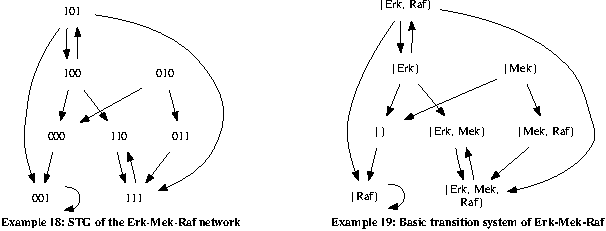
\includegraphics{figure17.pdf}}
\caption{The state transition graph \emph{``example18\_stg.pdf''} of the Erk-Mek-Raf network on the left
and the corresponding basic transition system on the right.}\label{Manual:figure17}\end{figure}

Since the choice of atomic propositions affects the expressiveness and conciseness of the model checking queries that users can formulate
we have decided to extend this basic transition system by some \emph{auxiliary variables}.
First, we add a proposition that states whether a variable is steady, i.e., whether its activity is equal to the value of its update function.
Those propositions add \emph{\_STEADY} to each variable, e.g. \emph{Mek\_STEADY} for \emph{Mek}.
Second, we add a proposition \emph{STEADYSTATE} that is true iff the respective state is a steady state.
Finally, we add a proposition \emph{SUCCESSORS=k} where \emph{k} is an integer,
that is true iff the respective state has exactly \emph{k} successors (excluding itself).
The propositions \emph{SUCCESSORS=0} and \emph{STEADYSTATE} are therefore equivalent.

\begin{notice}{note}{Note:}
The {\hyperref[Installation:installation-nusmv]{\emph{NuSMV}}} language is case sensitive.
\end{notice}

The transition system with the extended set of atomic propositions is shown in {\hyperref[Manual:figure18]{\emph{the figure below}}}.
\begin{figure}[htbp]
\centering
\capstart

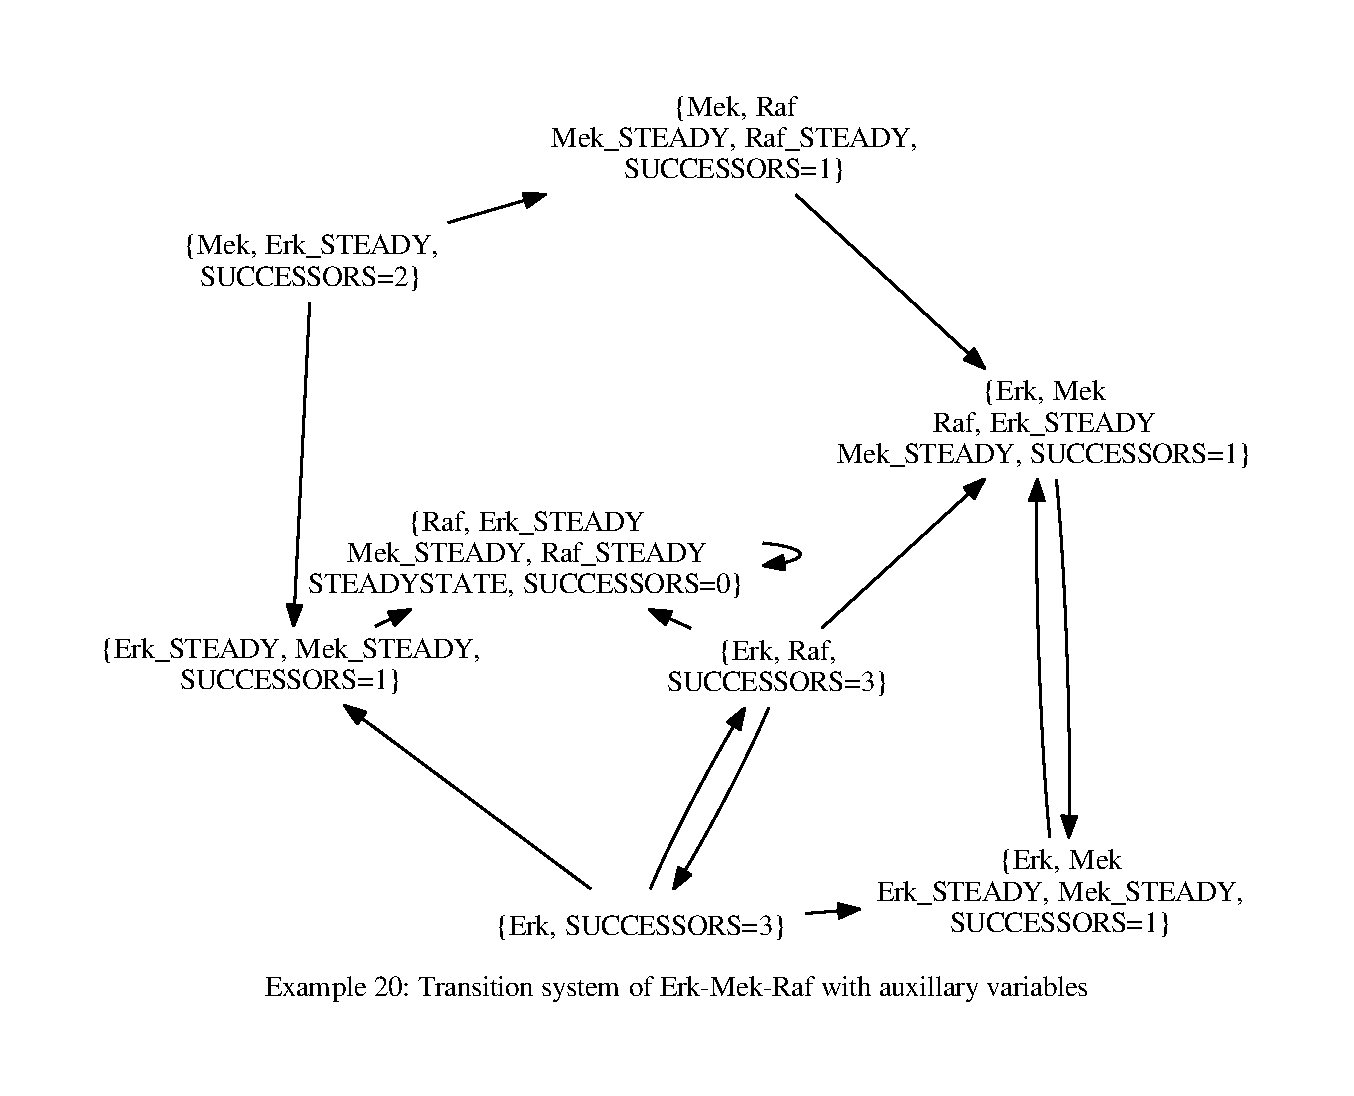
\includegraphics[height=7cm]{figure18.pdf}
\caption{The extended transition system for the Erk-Mek-Raf network.}\label{Manual:figure18}\end{figure}


\subsection{LTL model checking}
\label{Manual:ltl-model-checking}
Apart from a transition system, a model checking problem requires a \emph{temporal specification}.
Since \emph{PyBoolNet 2.11} uses {\hyperref[Installation:installation-nusmv]{\emph{NuSMV}}} for solving model checking problems, two specification languages are available:
\emph{linear time logic} (LTL) and \emph{computational tree logic} (CTL).

LTL specifications are statements about the sequence of events that are expressed in terms of atomic propositions and temporal operators.
A LTL specification is either true or false for a given linear sequence, i.e., infinite path, in a given transition system.
The basic temporal operators for LTL are:
\begin{itemize}
\item {} 
\emph{F(..)} which means \emph{finally}

\item {} 
\emph{G(..)} which means \emph{globally}

\item {} 
\emph{{[}..U..{]}} which means \emph{until}

\item {} 
\emph{X(..)} which means \emph{next}

\end{itemize}

LTL statements may be combined by the usual logical operators which are:
\begin{itemize}
\item {} 
\emph{\textbar{}} which means \emph{disjunction}

\item {} 
\emph{\&} which means \emph{conjunction}

\item {} 
\emph{!} which means \emph{negation}

\end{itemize}

in {\hyperref[Installation:installation-nusmv]{\emph{NuSMV}}} syntax.
For a formal definition of LTL formulas see for example {\hyperref[Bibliography:baier2008]{\emph{Baier2008}}}.

Finally, model checking problems allow the user to specify some states of the transition system to be \emph{initial}.
A LTL specification is then defined to be true for a transition system with initial states iff every path that starts from an initial state
satisfies the LTL specification.

As an example consider again the Erk-Mek-Raf network {\hyperref[Manual:figure17]{\emph{from above}}}.
Let us query whether along every path in its transition system there is eventually a state in which \emph{Raf} is activated:

\begin{Verbatim}[commandchars=\\\{\}]
\PYG{g+gp}{\PYGZgt{}\PYGZgt{}\PYGZgt{} }\PYG{k+kn}{from} \PYG{n+nn}{PyBoolNet} \PYG{k+kn}{import} \PYG{n}{ModelChecking} \PYG{k}{as} \PYG{n}{MC}
\PYG{g+gp}{\PYGZgt{}\PYGZgt{}\PYGZgt{} }\PYG{n}{init} \PYG{o}{=} \PYG{l+s}{\PYGZdq{}}\PYG{l+s}{INIT TRUE}\PYG{l+s}{\PYGZdq{}}
\PYG{g+gp}{\PYGZgt{}\PYGZgt{}\PYGZgt{} }\PYG{n}{spec} \PYG{o}{=} \PYG{l+s}{\PYGZdq{}}\PYG{l+s}{LTLSPEC F(Raf)}\PYG{l+s}{\PYGZdq{}}
\PYG{g+gp}{\PYGZgt{}\PYGZgt{}\PYGZgt{} }\PYG{n}{update} \PYG{o}{=} \PYG{l+s}{\PYGZdq{}}\PYG{l+s}{asynchronous}\PYG{l+s}{\PYGZdq{}}
\PYG{g+gp}{\PYGZgt{}\PYGZgt{}\PYGZgt{} }\PYG{n}{answer} \PYG{o}{=} \PYG{n}{MC}\PYG{o}{.}\PYG{n}{check\PYGZus{}primes}\PYG{p}{(}\PYG{n}{primes}\PYG{p}{,} \PYG{n}{update}\PYG{p}{,} \PYG{n}{init}\PYG{p}{,} \PYG{n}{spec}\PYG{p}{)}
\PYG{g+gp}{\PYGZgt{}\PYGZgt{}\PYGZgt{} }\PYG{n}{answer}
\PYG{g+go}{True}
\end{Verbatim}

The first line imports the module {\hyperref[ModelChecking:modelchecking]{\emph{ModelChecking}}}.
The next line defines the initial states in {\hyperref[Installation:installation-nusmv]{\emph{NuSMV}}} syntax with the keyword \emph{INIT} to indicate an initial condition and
the expression \emph{TRUE} which evaluates to true in every state.
The next line starts with the keyword \emph{LTLSPEC} which must precede the definition of a LTL specification and the formula \emph{F(Raf)} which
states that eventually a state will be reached that is labeled by \emph{Raf}, i.e., in which \emph{Raf} is activated.
The fifth line calls the function {\hyperref[ModelChecking:check-primes]{\emph{check\_primes}}} which constructs the extended transition system and
uses {\hyperref[Installation:installation-nusmv]{\emph{NuSMV}}} to answer model checking queries.
Note that the function requires a parameter that specifies the update rule, i.e., either \emph{``asynchronous''}, \emph{``synchronous''} or \emph{``mixed''}
and that it returns a Boolean value.

Even for this small example network it is not trivial to see why \emph{True} is the correct answer,
because a brute force approach would require the enumeration of all paths but the transition system contains an infinite number of paths.
Convince yourself that every path eventually reaches the state 101 or the state 111 or the state 001.
In all cases \emph{Raf}, which is the third digit in the state string, is equal to 1 which is what \emph{F(Raf)} requires.
Hence \emph{True} is the correct answer.

The second example is a slightly more complicated \emph{reachability} query:

\begin{Verbatim}[commandchars=\\\{\}]
\PYG{g+gp}{\PYGZgt{}\PYGZgt{}\PYGZgt{} }\PYG{n}{spec} \PYG{o}{=} \PYG{l+s}{\PYGZdq{}}\PYG{l+s}{LTLSPEC F(Raf \PYGZam{} F(STEADYSTATE))}\PYG{l+s}{\PYGZdq{}}
\PYG{g+gp}{\PYGZgt{}\PYGZgt{}\PYGZgt{} }\PYG{n}{answer} \PYG{o}{=} \PYG{n}{MC}\PYG{o}{.}\PYG{n}{check\PYGZus{}primes}\PYG{p}{(}\PYG{n}{primes}\PYG{p}{,} \PYG{n}{update}\PYG{p}{,} \PYG{n}{init}\PYG{p}{,} \PYG{n}{spec}\PYG{p}{)}
\PYG{g+gp}{\PYGZgt{}\PYGZgt{}\PYGZgt{} }\PYG{n}{answer}
\PYG{g+go}{False}
\end{Verbatim}

The LTL formula queries whether every path will eventually come across a state in which \emph{Raf} is activated followed by a steady state.
Note that the formula asserts an order on the sequence of events: first \emph{Raf} and then \emph{STEADYSTATE}.
To see why the specification is false we only need to find one infinite path from an initial state that does not satisfy the LTL formula.
Since all states are initial the following path will do:

\begin{Verbatim}[commandchars=\\\{\}]
101 \PYGZhy{}\PYGZgt{} 100 \PYGZhy{}\PYGZgt{} 110 \PYGZhy{}\PYGZgt{} 111 \PYGZhy{}\PYGZgt{} 110 \PYGZhy{}\PYGZgt{} 111 \PYGZhy{}\PYGZgt{} 110 \PYGZhy{}\PYGZgt{} ...
\end{Verbatim}

The last two states, 111 and 110, are repeated for ever and neither is labeled with \emph{STEADYSTATE} in the extended transition system,
see {\hyperref[Manual:figure18]{\emph{this figure}}}.
Hence \emph{False} is the correct answer.

The third example specifies a proper subset of states as initial and queries the existence of \emph{sustained oscillations} in \emph{Raf}:

\begin{Verbatim}[commandchars=\\\{\}]
\PYG{g+gp}{\PYGZgt{}\PYGZgt{}\PYGZgt{} }\PYG{n}{init} \PYG{o}{=} \PYG{l+s}{\PYGZdq{}}\PYG{l+s}{INIT Erk \PYGZam{} SUCCESSORS\PYGZlt{}2}\PYG{l+s}{\PYGZdq{}}
\PYG{g+gp}{\PYGZgt{}\PYGZgt{}\PYGZgt{} }\PYG{n}{spec} \PYG{o}{=} \PYG{l+s}{\PYGZdq{}}\PYG{l+s}{LTLSPEC G(F(Raf) \PYGZam{} F(!Raf))}\PYG{l+s}{\PYGZdq{}}
\PYG{g+gp}{\PYGZgt{}\PYGZgt{}\PYGZgt{} }\PYG{n}{answer} \PYG{o}{=} \PYG{n}{MC}\PYG{o}{.}\PYG{n}{check\PYGZus{}primes}\PYG{p}{(}\PYG{n}{primes}\PYG{p}{,} \PYG{n}{update}\PYG{p}{,} \PYG{n}{init}\PYG{p}{,} \PYG{n}{spec}\PYG{p}{)}
\PYG{g+gp}{\PYGZgt{}\PYGZgt{}\PYGZgt{} }\PYG{n}{answer}
\PYG{g+go}{True}
\end{Verbatim}

Here, a state is initial iff \emph{Erk} is activated in it and the number of its successors - with respect to the given the update rule - is less than two.
The formula \emph{G((F(Raf) \& F(!Raf))} requires that however far down the sequence of states, i.e., \emph{globally},
it is true that \emph{Raf} will eventually be activated and also that \emph{Raf} will eventually be inhibited.
The extended transition system, see {\hyperref[Manual:figure18]{\emph{this figure}}}, shows that exactly three state are initial: 110, 011 and 111.
Any path starting in one of those state will eventually end in the infinite sequence:

\begin{Verbatim}[commandchars=\\\{\}]
111 \PYGZhy{}\PYGZgt{} 110 \PYGZhy{}\PYGZgt{} 111 \PYGZhy{}\PYGZgt{} 110 \PYGZhy{}\PYGZgt{} 111 \PYGZhy{}\PYGZgt{} ...
\end{Verbatim}

Hence, any path that starts in one of the initial states satisfies \emph{G((F(Raf) \& F(!Raf))}, i.e.,
a sustained oscillation in \emph{Raf}, and hence the truth of the query.

The fourth example involves another feature: the use of {\hyperref[Installation:installation-nusmv]{\emph{NuSMV}}} built-in functions, in this case \emph{count}:

\begin{Verbatim}[commandchars=\\\{\}]
\PYG{g+gp}{\PYGZgt{}\PYGZgt{}\PYGZgt{} }\PYG{n}{init} \PYG{o}{=} \PYG{l+s}{\PYGZdq{}}\PYG{l+s}{INIT Mek}\PYG{l+s}{\PYGZdq{}}
\PYG{g+gp}{\PYGZgt{}\PYGZgt{}\PYGZgt{} }\PYG{n}{spec} \PYG{o}{=} \PYG{l+s}{\PYGZdq{}}\PYG{l+s}{LTLSPEC G(count(Erk\PYGZus{}STEADY,Mek\PYGZus{}STEADY,Raf\PYGZus{}STEADY)\PYGZgt{}=2)}\PYG{l+s}{\PYGZdq{}}
\PYG{g+gp}{\PYGZgt{}\PYGZgt{}\PYGZgt{} }\PYG{n}{answer} \PYG{o}{=} \PYG{n}{MC}\PYG{o}{.}\PYG{n}{check\PYGZus{}primes}\PYG{p}{(}\PYG{n}{primes}\PYG{p}{,} \PYG{n}{update}\PYG{p}{,} \PYG{n}{init}\PYG{p}{,} \PYG{n}{spec}\PYG{p}{)}
\PYG{g+gp}{\PYGZgt{}\PYGZgt{}\PYGZgt{} }\PYG{n}{answer}
\PYG{g+go}{False}
\end{Verbatim}

The LTL formula also uses the auxiliary variables \emph{Erk\_STEADY}, \emph{Mek\_STEADY} and \emph{Raf\_STEADY} which are true in states in which the respective variables
are equal to the values of their update functions.
The formula states that along any path that starts from an initial state at least two of the variables \emph{Erk}, \emph{Mek} and \emph{Raf} are steady.
Since the query is false there must be a path that does not satisfy the specifications, for example this one:

\begin{Verbatim}[commandchars=\\\{\}]
010 \PYGZhy{}\PYGZgt{} 011 \PYGZhy{}\PYGZgt{} 111 \PYGZhy{}\PYGZgt{} 110 \PYGZhy{}\PYGZgt{} 111 \PYGZhy{}\PYGZgt{} 110 \PYGZhy{}\PYGZgt{} ...
\end{Verbatim}

It does not satisfy the LTL formula because in the state 010 only \emph{Erk} is steady and
hence \emph{count(...)} which counts the number of true expressions is equal to one and hence \emph{G(count(...)\textgreater{}=2)} is false.
See the {\hyperref[Installation:installation-nusmv]{\emph{NuSMV}}} manual for more built-in functions like \emph{count()}.

The existence of so-called \emph{counterexamples} is essential to LTL model checking
and {\hyperref[Installation:installation-nusmv]{\emph{NuSMV}}} can be asked to return one if it finds one.


\subsection{LTL counterexamples}
\label{Manual:ltl-counterexamples}
If a LTL query is false then {\hyperref[Installation:installation-nusmv]{\emph{NuSMV}}} can return a finite path that proves that the formula is false.

\begin{notice}{note}{Note:}
Since the transition systems of Boolean networks are finite, a counterexample will always be a finite sequence of states -
possibly ending in a cycle.
For a justification, see for example {\hyperref[Bibliography:baier2008]{\emph{Baier2008}}} Sec. 5.2.
\end{notice}

To return a counterexample use the function {\hyperref[ModelChecking:check-primes-with-counterexample]{\emph{check\_primes\_with\_counterexample}}}.
The function returns the answer and a counterexample.
Reconsider the following query, which we know is false, from above:

\begin{Verbatim}[commandchars=\\\{\}]
\PYG{g+gp}{\PYGZgt{}\PYGZgt{}\PYGZgt{} }\PYG{n}{init} \PYG{o}{=} \PYG{l+s}{\PYGZdq{}}\PYG{l+s}{INIT TRUE}\PYG{l+s}{\PYGZdq{}}
\PYG{g+gp}{\PYGZgt{}\PYGZgt{}\PYGZgt{} }\PYG{n}{spec} \PYG{o}{=} \PYG{l+s}{\PYGZdq{}}\PYG{l+s}{LTLSPEC F(Raf \PYGZam{} F(STEADYSTATE))}\PYG{l+s}{\PYGZdq{}}
\end{Verbatim}

To retrieve the answer and a counterexample call:

\begin{Verbatim}[commandchars=\\\{\}]
\PYG{g+gp}{\PYGZgt{}\PYGZgt{}\PYGZgt{} }\PYG{n}{answer}\PYG{p}{,} \PYG{n}{counterex} \PYG{o}{=} \PYG{n}{MC}\PYG{o}{.}\PYG{n}{check\PYGZus{}primes\PYGZus{}with\PYGZus{}counterexample}\PYG{p}{(}\PYG{n}{primes}\PYG{p}{,} \PYG{n}{update}\PYG{p}{,} \PYG{n}{init}\PYG{p}{,} \PYG{n}{spec}\PYG{p}{)}
\end{Verbatim}

The counterexample is a tuple of state dictionaries (recall {\hyperref[Manual:states-subspaces-paths]{\emph{states, subspaces and paths}}}) if the query is false
and \emph{None} in case it is true (in which case no counterexample exists).
Hence, a typical way to inspect a counterexample involves a Python if-statement:

\begin{Verbatim}[commandchars=\\\{\}]
\PYG{g+gp}{\PYGZgt{}\PYGZgt{}\PYGZgt{} }\PYG{k}{if} \PYG{n}{counterex}\PYG{p}{:}
\PYG{g+gp}{... }    \PYG{k}{print} \PYG{l+s}{\PYGZdq{}}\PYG{l+s}{ \PYGZhy{}\PYGZgt{} }\PYG{l+s}{\PYGZdq{}}\PYG{o}{.}\PYG{n}{join}\PYG{p}{(}\PYG{n}{STGs}\PYG{o}{.}\PYG{n}{state2str}\PYG{p}{(}\PYG{n}{x}\PYG{p}{)} \PYG{k}{for} \PYG{n}{x} \PYG{o+ow}{in} \PYG{n}{counterex}\PYG{p}{)}
\PYG{g+go}{100 \PYGZhy{}\PYGZgt{} 101 \PYGZhy{}\PYGZgt{} 100}
\end{Verbatim}

Here, {\hyperref[StateTransitionGraphs:state2str]{\emph{state2str}}} is a ``pretty print'' function contained in the module {\hyperref[StateTransitionGraphs:statetransitiongraphs]{\emph{StateTransitionGraphs}}}.
It generates a state string from a state dictionary.
An alternative way of inspecting counterexample is by {\hyperref[StateTransitionGraphs:add-style-path]{\emph{STGs.add\_style\_path}}}:

\begin{Verbatim}[commandchars=\\\{\}]
\PYG{g+gp}{\PYGZgt{}\PYGZgt{}\PYGZgt{} }\PYG{n}{stg} \PYG{o}{=} \PYG{n}{STGs}\PYG{o}{.}\PYG{n}{primes2stg}\PYG{p}{(}\PYG{n}{primes}\PYG{p}{,} \PYG{n}{update}\PYG{p}{)}
\PYG{g+gp}{\PYGZgt{}\PYGZgt{}\PYGZgt{} }\PYG{n}{STGs}\PYG{o}{.}\PYG{n}{add\PYGZus{}style\PYGZus{}path}\PYG{p}{(}\PYG{n}{stg}\PYG{p}{,} \PYG{n}{counterex}\PYG{p}{,} \PYG{l+s}{\PYGZdq{}}\PYG{l+s}{red}\PYG{l+s}{\PYGZdq{}}\PYG{p}{)}
\PYG{g+gp}{\PYGZgt{}\PYGZgt{}\PYGZgt{} }\PYG{n}{stg}\PYG{o}{.}\PYG{n}{graph}\PYG{p}{[}\PYG{l+s}{\PYGZdq{}}\PYG{l+s}{label}\PYG{l+s}{\PYGZdq{}}\PYG{p}{]} \PYG{o}{=} \PYG{l+s}{\PYGZdq{}}\PYG{l+s}{Example 19: A LTL counterexample}\PYG{l+s}{\PYGZdq{}}
\PYG{g+gp}{\PYGZgt{}\PYGZgt{}\PYGZgt{} }\PYG{n}{STGs}\PYG{o}{.}\PYG{n}{stg2image}\PYG{p}{(}\PYG{n}{stg}\PYG{p}{,} \PYG{l+s}{\PYGZdq{}}\PYG{l+s}{example19\PYGZus{}stg.pdf}\PYG{l+s}{\PYGZdq{}}\PYG{p}{)}
\end{Verbatim}
\begin{figure}[htbp]
\centering
\capstart

\scalebox{0.600000}{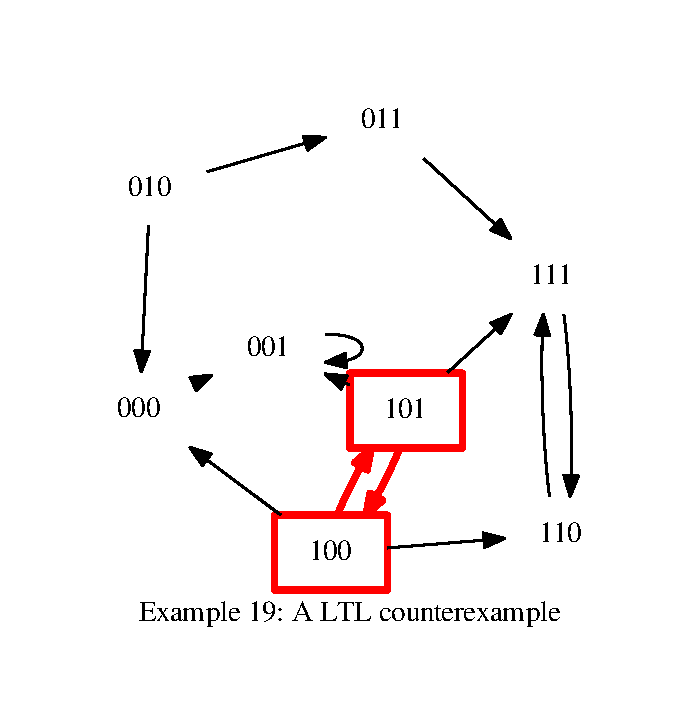
\includegraphics{figure19.pdf}}
\caption{The state transition graph \emph{``example18\_stg.pdf''} of the Erk-Mek-Raf network with a path style that indicates a counterexample to
the LTL query with all states being initial and the formula \emph{F(Raf \& F(STEADYSTATE))}.}\label{Manual:figure19}\end{figure}

A second alternative is to generate an animated \emph{gif} of the changing activities in each state
and using {\hyperref[InteractionGraphs:activities2animation]{\emph{IGs.activities2animation}}}:

\begin{Verbatim}[commandchars=\\\{\}]
\PYG{g+gp}{\PYGZgt{}\PYGZgt{}\PYGZgt{} }\PYG{n}{igraph} \PYG{o}{=} \PYG{n}{IGs}\PYG{o}{.}\PYG{n}{primes2igraph}\PYG{p}{(}\PYG{n}{primes}\PYG{p}{)}
\PYG{g+gp}{\PYGZgt{}\PYGZgt{}\PYGZgt{} }\PYG{n}{IGs}\PYG{o}{.}\PYG{n}{activities2animation}\PYG{p}{(}\PYG{n}{igraph}\PYG{p}{,} \PYG{n}{counterex}\PYG{p}{,} \PYG{l+s}{\PYGZdq{}}\PYG{l+s}{counterexample.gif}\PYG{l+s}{\PYGZdq{}}\PYG{p}{)}
\end{Verbatim}


\subsection{CTL model checking}
\label{Manual:ctl-model-checking}
{\hyperref[Installation:installation-nusmv]{\emph{NuSMV}}} can also solve model checking problems that involve \emph{computation tree logic} (CTL).
CTL formulas are constructed like LTL formulas but the temporal operators \emph{F}, \emph{G}, \emph{X} and \emph{U} must be quantified by \emph{E} which means \emph{for some path}
or \emph{A} which means \emph{for all paths}.
A CTL formula is not evaluated for paths but for trees of successors rooted in some initial state.

\begin{notice}{note}{Note:}
Some properties can be specified in LTL or CTL, other properties can only be stated in either LTL or CTL.
See Sec. 6.3 in {\hyperref[Bibliography:baier2008]{\emph{Baier2008}}} for a discussion of the expressiveness of CTL and LTL.
\end{notice}

Consider the following toy model of cell proliferation:

\begin{Verbatim}[commandchars=\\\{\}]
\PYG{g+gp}{\PYGZgt{}\PYGZgt{}\PYGZgt{} }\PYG{n}{bnet} \PYG{o}{=} \PYG{p}{[}\PYG{l+s}{\PYGZdq{}}\PYG{l+s}{GrowthFactor,  0}\PYG{l+s}{\PYGZdq{}}\PYG{p}{,}
\PYG{g+gp}{... }        \PYG{l+s}{\PYGZdq{}}\PYG{l+s}{Proliferation, GrowthFactor \textbar{} Proliferation \PYGZam{} !DNAdamage}\PYG{l+s}{\PYGZdq{}}\PYG{p}{,}
\PYG{g+gp}{... }        \PYG{l+s}{\PYGZdq{}}\PYG{l+s}{DNAdamage,     !GrowthFactor \PYGZam{} DNAdamage}\PYG{l+s}{\PYGZdq{}}\PYG{p}{]}
\PYG{g+gp}{\PYGZgt{}\PYGZgt{}\PYGZgt{} }\PYG{n}{bnet} \PYG{o}{=} \PYG{l+s}{\PYGZdq{}}\PYG{l+s+se}{\PYGZbs{}n}\PYG{l+s}{\PYGZdq{}}\PYG{o}{.}\PYG{n}{join}\PYG{p}{(}\PYG{n}{bnet}\PYG{p}{)}
\PYG{g+gp}{\PYGZgt{}\PYGZgt{}\PYGZgt{} }\PYG{n}{primes} \PYG{o}{=} \PYG{n}{FEX}\PYG{o}{.}\PYG{n}{bnet2primes}\PYG{p}{(}\PYG{n}{bnet}\PYG{p}{)}
\PYG{g+gp}{\PYGZgt{}\PYGZgt{}\PYGZgt{} }\PYG{n}{update} \PYG{o}{=} \PYG{l+s}{\PYGZdq{}}\PYG{l+s}{asynchronous}\PYG{l+s}{\PYGZdq{}}
\end{Verbatim}

Suppose we want to find out whether the presence of \emph{GrowthFactor} implies the possibility of \emph{Proliferation}.
By ``possibility'' we mean that there is a path that leads to a state in which proliferation is activated.
Let us first determine whether this property holds in the network above by drawing the state transition graph with
the initial states and the proliferation states highlighted by filled rectangles and a subgraph, respectively:

\begin{Verbatim}[commandchars=\\\{\}]
\PYG{g+gp}{\PYGZgt{}\PYGZgt{}\PYGZgt{} }\PYG{n}{stg} \PYG{o}{=} \PYG{n}{STGs}\PYG{o}{.}\PYG{n}{primes2stg}\PYG{p}{(}\PYG{n}{primes}\PYG{p}{,} \PYG{n}{update}\PYG{p}{)}
\PYG{g+gp}{\PYGZgt{}\PYGZgt{}\PYGZgt{} }\PYG{k}{for} \PYG{n}{x} \PYG{o+ow}{in} \PYG{n}{stg}\PYG{o}{.}\PYG{n}{nodes}\PYG{p}{(}\PYG{p}{)}\PYG{p}{:}
\PYG{g+gp}{... }    \PYG{n}{x\PYGZus{}dict} \PYG{o}{=} \PYG{n}{STGs}\PYG{o}{.}\PYG{n}{state2dict}\PYG{p}{(}\PYG{n}{primes}\PYG{p}{,} \PYG{n}{x}\PYG{p}{)}
\PYG{g+gp}{... }    \PYG{k}{if} \PYG{n}{x\PYGZus{}dict}\PYG{p}{[}\PYG{l+s}{\PYGZdq{}}\PYG{l+s}{GrowthFactor}\PYG{l+s}{\PYGZdq{}}\PYG{p}{]}\PYG{p}{:}
\PYG{g+gp}{... }        \PYG{n}{stg}\PYG{o}{.}\PYG{n}{node}\PYG{p}{[}\PYG{n}{x}\PYG{p}{]}\PYG{p}{[}\PYG{l+s}{\PYGZdq{}}\PYG{l+s}{style}\PYG{l+s}{\PYGZdq{}}\PYG{p}{]} \PYG{o}{=} \PYG{l+s}{\PYGZdq{}}\PYG{l+s}{filled}\PYG{l+s}{\PYGZdq{}}
\PYG{g+gp}{... }        \PYG{n}{stg}\PYG{o}{.}\PYG{n}{node}\PYG{p}{[}\PYG{n}{x}\PYG{p}{]}\PYG{p}{[}\PYG{l+s}{\PYGZdq{}}\PYG{l+s}{fillcolor}\PYG{l+s}{\PYGZdq{}}\PYG{p}{]} \PYG{o}{=} \PYG{l+s}{\PYGZdq{}}\PYG{l+s}{gray}\PYG{l+s}{\PYGZdq{}}
\PYG{g+gp}{\PYGZgt{}\PYGZgt{}\PYGZgt{} }\PYG{n}{sub} \PYG{o}{=} \PYG{p}{(}\PYG{p}{\PYGZob{}}\PYG{l+s}{\PYGZdq{}}\PYG{l+s}{Proliferation}\PYG{l+s}{\PYGZdq{}}\PYG{p}{:}\PYG{l+m+mi}{1}\PYG{p}{\PYGZcb{}}\PYG{p}{,}\PYG{p}{\PYGZob{}}\PYG{l+s}{\PYGZdq{}}\PYG{l+s}{label}\PYG{l+s}{\PYGZdq{}}\PYG{p}{:}\PYG{l+s}{\PYGZdq{}}\PYG{l+s}{proliferation}\PYG{l+s}{\PYGZdq{}}\PYG{p}{\PYGZcb{}}\PYG{p}{)}
\PYG{g+gp}{\PYGZgt{}\PYGZgt{}\PYGZgt{} }\PYG{n}{STGs}\PYG{o}{.}\PYG{n}{add\PYGZus{}style\PYGZus{}subspaces}\PYG{p}{(}\PYG{n}{stg}\PYG{p}{,} \PYG{p}{[}\PYG{n}{sub}\PYG{p}{]}\PYG{p}{)}
\PYG{g+gp}{\PYGZgt{}\PYGZgt{}\PYGZgt{} }\PYG{n}{stg}\PYG{o}{.}\PYG{n}{graph}\PYG{p}{[}\PYG{l+s}{\PYGZdq{}}\PYG{l+s}{label}\PYG{l+s}{\PYGZdq{}}\PYG{p}{]} \PYG{o}{=} \PYG{l+s}{\PYGZdq{}}\PYG{l+s}{Example 20: STG of the Proliferation network}\PYG{l+s}{\PYGZdq{}}
\PYG{g+gp}{\PYGZgt{}\PYGZgt{}\PYGZgt{} }\PYG{n}{STGs}\PYG{o}{.}\PYG{n}{stg2image}\PYG{p}{(}\PYG{n}{stg}\PYG{p}{,} \PYG{l+s}{\PYGZdq{}}\PYG{l+s}{example20\PYGZus{}stg.pdf}\PYG{l+s}{\PYGZdq{}}\PYG{p}{)}
\end{Verbatim}

It is easy to see, in the {\hyperref[Manual:figure20]{\emph{figure below}}}, that for every initial state there is a path to a proliferation state.
There are two initial states in which \emph{Proliferation} is inhibited, namely \emph{110} and \emph{010}.
For each there is a path leading to a state in which \emph{Proliferation} is activated, namely:

\begin{Verbatim}[commandchars=\\\{\}]
110 \PYGZhy{}\PYGZgt{} 111 and 010 \PYGZhy{}\PYGZgt{} 011
\end{Verbatim}

Perhaps surprisingly, this property can not be formulated in LTL.
The LTL formula is \emph{F(Proliferation)}, for example, requires that \emph{all paths} lead to a proliferation state which is
not the same as \emph{some paths} lead to proliferation.
In fact, the property \emph{F(Proliferation)} is false, as {\hyperref[Manual:figure21]{\emph{the figure below}}} for the following counterexample demonstrates:

\begin{Verbatim}[commandchars=\\\{\}]
\PYG{g+gp}{\PYGZgt{}\PYGZgt{}\PYGZgt{} }\PYG{n}{init} \PYG{o}{=} \PYG{l+s}{\PYGZdq{}}\PYG{l+s}{INIT GrowthFactor}\PYG{l+s}{\PYGZdq{}}
\PYG{g+gp}{\PYGZgt{}\PYGZgt{}\PYGZgt{} }\PYG{n}{spec} \PYG{o}{=} \PYG{l+s}{\PYGZdq{}}\PYG{l+s}{LTLSPEC F(Proliferation)}\PYG{l+s}{\PYGZdq{}}
\PYG{g+gp}{\PYGZgt{}\PYGZgt{}\PYGZgt{} }\PYG{n}{answer}\PYG{p}{,} \PYG{n}{counterex} \PYG{o}{=} \PYG{n}{MC}\PYG{o}{.}\PYG{n}{check\PYGZus{}primes\PYGZus{}with\PYGZus{}counterexample}\PYG{p}{(}\PYG{n}{primes}\PYG{p}{,} \PYG{n}{update}\PYG{p}{,} \PYG{n}{init}\PYG{p}{,} \PYG{n}{spec}\PYG{p}{)}
\PYG{g+gp}{\PYGZgt{}\PYGZgt{}\PYGZgt{} }\PYG{n}{answer}
\PYG{g+go}{False}
\PYG{g+gp}{\PYGZgt{}\PYGZgt{}\PYGZgt{} }\PYG{n}{STGs}\PYG{o}{.}\PYG{n}{add\PYGZus{}style\PYGZus{}path}\PYG{p}{(}\PYG{n}{stg}\PYG{p}{,} \PYG{n}{counterex}\PYG{p}{,} \PYG{l+s}{\PYGZdq{}}\PYG{l+s}{red}\PYG{l+s}{\PYGZdq{}}\PYG{p}{)}
\PYG{g+gp}{\PYGZgt{}\PYGZgt{}\PYGZgt{} }\PYG{n}{stg}\PYG{o}{.}\PYG{n}{graph}\PYG{p}{[}\PYG{l+s}{\PYGZdq{}}\PYG{l+s}{label}\PYG{l+s}{\PYGZdq{}}\PYG{p}{]} \PYG{o}{=} \PYG{l+s}{\PYGZdq{}}\PYG{l+s}{Example 21: Counterexample}\PYG{l+s}{\PYGZdq{}}
\PYG{g+gp}{\PYGZgt{}\PYGZgt{}\PYGZgt{} }\PYG{n}{STGs}\PYG{o}{.}\PYG{n}{stg2image}\PYG{p}{(}\PYG{n}{stg}\PYG{p}{,} \PYG{l+s}{\PYGZdq{}}\PYG{l+s}{example21\PYGZus{}stg.pdf}\PYG{l+s}{\PYGZdq{}}\PYG{p}{)}
\end{Verbatim}
\begin{figure}[htbp]
\centering
\capstart

\scalebox{0.600000}{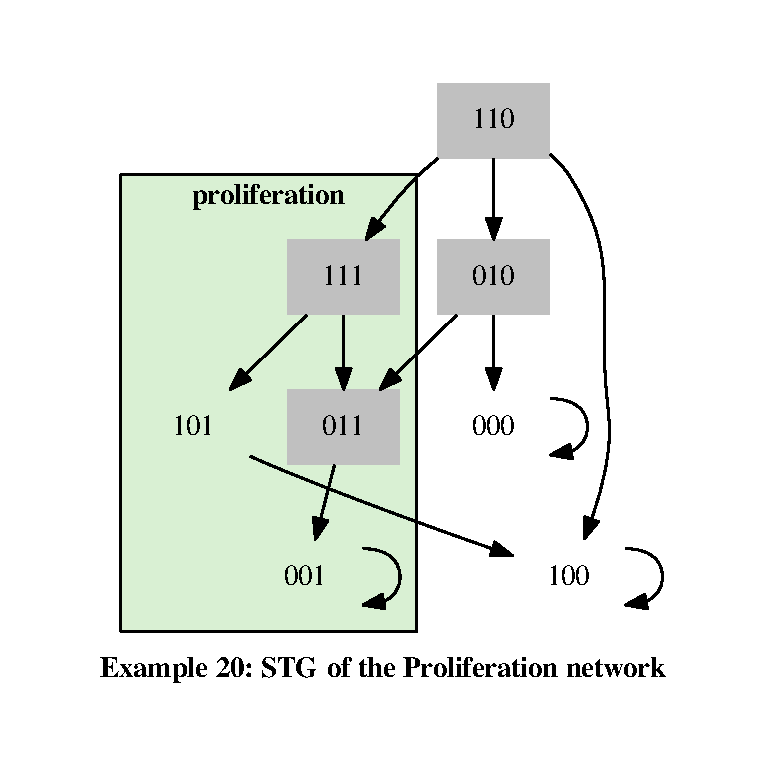
\includegraphics{figure20.pdf}}
\caption{The state transition graph \emph{``example20\_stg.pdf''} of the Proliferation network with initial states highlighted by gray rectangles
and proliferation states gathered in a subgraph.}\label{Manual:figure20}\end{figure}
\begin{figure}[htbp]
\centering
\capstart

\scalebox{0.600000}{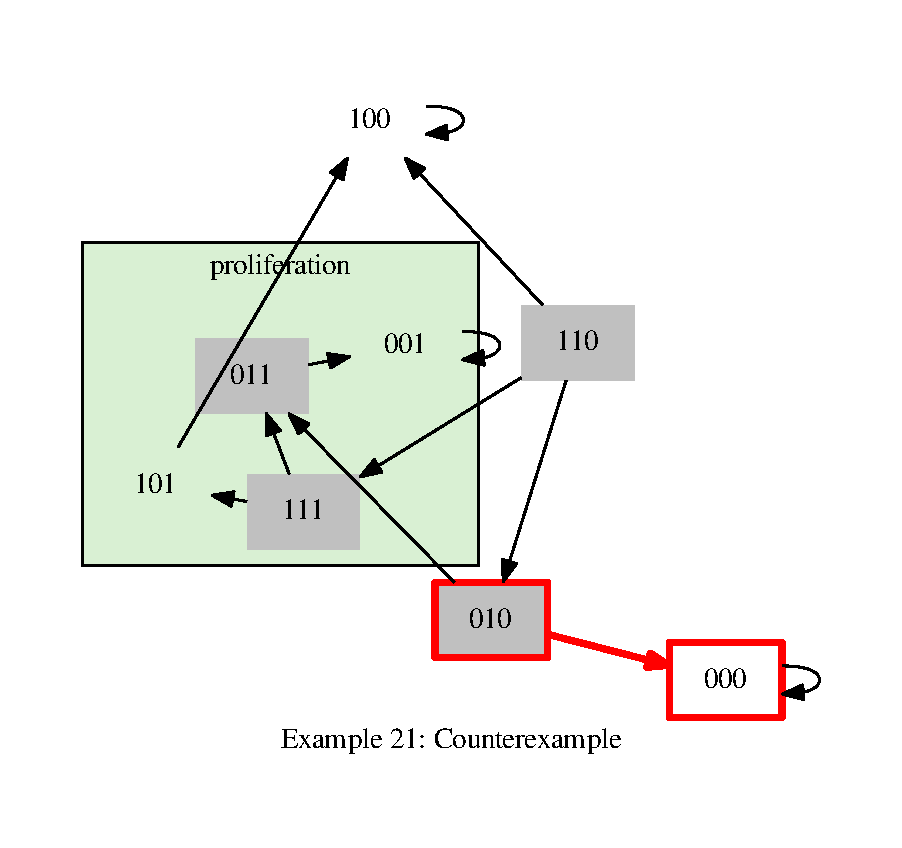
\includegraphics{figure21.pdf}}
\caption{The state transition graph \emph{``example21\_stg.pdf''} of the Proliferation network with a counterexample highlighted by path.}\label{Manual:figure21}\end{figure}

The property can, however, be formulated in CTL using the existential quantifier:

\begin{Verbatim}[commandchars=\\\{\}]
\PYG{g+gp}{\PYGZgt{}\PYGZgt{}\PYGZgt{} }\PYG{n}{spec} \PYG{o}{=} \PYG{l+s}{\PYGZdq{}}\PYG{l+s}{CTLSPEC EF(Proliferation)}\PYG{l+s}{\PYGZdq{}}
\PYG{g+gp}{\PYGZgt{}\PYGZgt{}\PYGZgt{} }\PYG{n}{answer} \PYG{o}{=} \PYG{n}{MC}\PYG{o}{.}\PYG{n}{check\PYGZus{}primes}\PYG{p}{(}\PYG{n}{primes}\PYG{p}{,} \PYG{n}{update}\PYG{p}{,} \PYG{n}{init}\PYG{p}{,} \PYG{n}{spec}\PYG{p}{)}
\PYG{g+go}{True}
\end{Verbatim}

\begin{notice}{note}{Note:}
The LTL formula \emph{F(Proliferation)} is equivalent to the CTL formula \emph{AF(Proliferation)}.
In general, however, there are LTL formulas for which no equivalent CTL formula exists, and vice versa.
\end{notice}

CTL model checking is also required when querying properties about the \emph{attractors} of the state transition graph.
Attractors are defined to be the \emph{terminal SCCs} of the STG or, equivalently, they are its \emph{minimal trap sets}.
For a formal definition see for example {\hyperref[Bibliography:klarner2015approx]{\emph{Klarner2015(b)}}} Sec. 2.2.

Suppose we want to find out whether, for the initial states defined \emph{Proliferation},
all attractors are located in the subset of states that are defined by \emph{!DNAdamage}.
In English, this property states that ``along any path starting from any initial state it is possible to reach a state from
which all reachable states satisfy \emph{!DNAdamage}''.
In CTL, it can be formulated using the \emph{AG(EF(AG(...)))} query pattern where ''...'' is the condition that describes the attractor states:

\begin{Verbatim}[commandchars=\\\{\}]
\PYG{g+gp}{\PYGZgt{}\PYGZgt{}\PYGZgt{} }\PYG{n}{init} \PYG{o}{=} \PYG{l+s}{\PYGZdq{}}\PYG{l+s}{INIT Proliferation}\PYG{l+s}{\PYGZdq{}}
\PYG{g+gp}{\PYGZgt{}\PYGZgt{}\PYGZgt{} }\PYG{n}{condition} \PYG{o}{=} \PYG{l+s}{\PYGZdq{}}\PYG{l+s}{!DNAdamage}\PYG{l+s}{\PYGZdq{}}
\PYG{g+gp}{\PYGZgt{}\PYGZgt{}\PYGZgt{} }\PYG{n}{spec} \PYG{o}{=} \PYG{l+s}{\PYGZdq{}}\PYG{l+s}{CTLSPEC AG(EF(AG(}\PYG{l+s+si}{\PYGZpc{}s}\PYG{l+s}{)))}\PYG{l+s}{\PYGZdq{}}\PYG{o}{\PYGZpc{}}\PYG{n}{condition}
\PYG{g+gp}{\PYGZgt{}\PYGZgt{}\PYGZgt{} }\PYG{n}{answer} \PYG{o}{=} \PYG{n}{MC}\PYG{o}{.}\PYG{n}{check\PYGZus{}primes}\PYG{p}{(}\PYG{n}{primes}\PYG{p}{,} \PYG{n}{update}\PYG{p}{,} \PYG{n}{init}\PYG{p}{,} \PYG{n}{spec}\PYG{p}{)}
\PYG{g+go}{True}
\end{Verbatim}

Other frequently used conditions are \emph{STEADYSTATE} to query whether all attractors are steady states:

\begin{Verbatim}[commandchars=\\\{\}]
\PYG{g+gp}{\PYGZgt{}\PYGZgt{}\PYGZgt{} }\PYG{n}{init} \PYG{o}{=} \PYG{l+s}{\PYGZdq{}}\PYG{l+s}{INIT Proliferation}\PYG{l+s}{\PYGZdq{}}
\PYG{g+gp}{\PYGZgt{}\PYGZgt{}\PYGZgt{} }\PYG{n}{condition} \PYG{o}{=} \PYG{l+s}{\PYGZdq{}}\PYG{l+s}{STEADYSTATE}\PYG{l+s}{\PYGZdq{}}
\PYG{g+gp}{\PYGZgt{}\PYGZgt{}\PYGZgt{} }\PYG{n}{spec} \PYG{o}{=} \PYG{l+s}{\PYGZdq{}}\PYG{l+s}{CTLSPEC AG(EF(AG(}\PYG{l+s+si}{\PYGZpc{}s}\PYG{l+s}{)))}\PYG{l+s}{\PYGZdq{}}\PYG{o}{\PYGZpc{}}\PYG{n}{condition}
\PYG{g+gp}{\PYGZgt{}\PYGZgt{}\PYGZgt{} }\PYG{n}{answer} \PYG{o}{=} \PYG{n}{MC}\PYG{o}{.}\PYG{n}{check\PYGZus{}primes}\PYG{p}{(}\PYG{n}{primes}\PYG{p}{,} \PYG{n}{update}\PYG{p}{,} \PYG{n}{init}\PYG{p}{,} \PYG{n}{spec}\PYG{p}{)}
\PYG{g+go}{True}
\end{Verbatim}

or disjunctions and conjunctions of basic propositions:

\begin{Verbatim}[commandchars=\\\{\}]
\PYG{g+gp}{\PYGZgt{}\PYGZgt{}\PYGZgt{} }\PYG{n}{init} \PYG{o}{=} \PYG{l+s}{\PYGZdq{}}\PYG{l+s}{INIT Proliferation}\PYG{l+s}{\PYGZdq{}}
\PYG{g+gp}{\PYGZgt{}\PYGZgt{}\PYGZgt{} }\PYG{n}{condition} \PYG{o}{=} \PYG{l+s}{\PYGZdq{}}\PYG{l+s}{STEADYSTATE \textbar{} (!Proliferation \PYGZam{} DNAdamage)}\PYG{l+s}{\PYGZdq{}}
\PYG{g+gp}{\PYGZgt{}\PYGZgt{}\PYGZgt{} }\PYG{n}{spec} \PYG{o}{=} \PYG{l+s}{\PYGZdq{}}\PYG{l+s}{CTLSPEC AG(EF(AG(}\PYG{l+s+si}{\PYGZpc{}s}\PYG{l+s}{)))}\PYG{l+s}{\PYGZdq{}}\PYG{o}{\PYGZpc{}}\PYG{n}{condition}
\PYG{g+gp}{\PYGZgt{}\PYGZgt{}\PYGZgt{} }\PYG{n}{answer} \PYG{o}{=} \PYG{n}{MC}\PYG{o}{.}\PYG{n}{check\PYGZus{}primes}\PYG{p}{(}\PYG{n}{primes}\PYG{p}{,} \PYG{n}{update}\PYG{p}{,} \PYG{n}{init}\PYG{p}{,} \PYG{n}{spec}\PYG{p}{)}
\PYG{g+go}{True}
\end{Verbatim}

\begin{notice}{note}{Note:}
The CTL formula \emph{AG(EF(AG(STEADYSTATE)))} is equivalent to \emph{AG(EF(STEADYSTATE)} because if a steady is steady then it has no successors.
\end{notice}

\begin{notice}{note}{Note:}
To query whether \emph{there is} an attractor of a certain type reachable from every initial state,
rather than whether \emph{all} attractors are of a certain type, use the query pattern \emph{EF(AG(...))} instead of \emph{AG(EF(AG(...)))}.
\end{notice}


\subsection{CTL counterexamples}
\label{Manual:ctl-counterexamples}
If a CTL formula is false then {\hyperref[Installation:installation-nusmv]{\emph{NuSMV}}} can return a finite path that starts with an initial state that does not satisfy the formula.

\begin{notice}{note}{Note:}
There is a fundamental difference between LTL and CTL counterexamples.
LTL counterexamples prove that the formula is false in the sense that any transition system that contains that path will not satisfy the formula.
CTL counterexamples, on the other hand, can not be used as general proofs.
They merely contain an initial state that does not satisfy the formula \emph{in the given transition system}.
\end{notice}

Suppose we want to find out whether each initial states defined by \emph{Proliferation} has a successor state that also satisfies \emph{Proliferation}.
To define this property we use the CTL operator \emph{EX}:

\begin{Verbatim}[commandchars=\\\{\}]
\PYG{g+gp}{\PYGZgt{}\PYGZgt{}\PYGZgt{} }\PYG{n}{init} \PYG{l+s}{\PYGZdq{}}\PYG{l+s}{INIT Proliferation}\PYG{l+s}{\PYGZdq{}}
\PYG{g+gp}{\PYGZgt{}\PYGZgt{}\PYGZgt{} }\PYG{n}{spec} \PYG{l+s}{\PYGZdq{}}\PYG{l+s}{CTLSPEC EX(Proliferation)}\PYG{l+s}{\PYGZdq{}}
\PYG{g+gp}{\PYGZgt{}\PYGZgt{}\PYGZgt{} }\PYG{n}{answer} \PYG{o}{=} \PYG{n}{MC}\PYG{o}{.}\PYG{n}{check\PYGZus{}primes}\PYG{p}{(}\PYG{n}{primes}\PYG{p}{,} \PYG{n}{update}\PYG{p}{,} \PYG{n}{init}\PYG{p}{,} \PYG{n}{spec}\PYG{p}{)}
\PYG{g+go}{False}
\PYG{g+gp}{\PYGZgt{}\PYGZgt{}\PYGZgt{} }\PYG{n}{answer}\PYG{p}{,} \PYG{n}{counterex} \PYG{o}{=} \PYG{n}{MC}\PYG{o}{.}\PYG{n}{check\PYGZus{}primes\PYGZus{}with\PYGZus{}counterexample}\PYG{p}{(}\PYG{n}{primes}\PYG{p}{,} \PYG{n}{update}\PYG{p}{,} \PYG{n}{init}\PYG{p}{,} \PYG{n}{spec}\PYG{p}{)}
\PYG{g+gp}{\PYGZgt{}\PYGZgt{}\PYGZgt{} }\PYG{n}{counterex}
\PYG{g+go}{(\PYGZob{}\PYGZsq{}DNAdamage\PYGZsq{}: 1, \PYGZsq{}Proliferation\PYGZsq{}: 1, \PYGZsq{}GrowthFactor\PYGZsq{}: 0\PYGZcb{},)}
\PYG{g+gp}{\PYGZgt{}\PYGZgt{}\PYGZgt{} }\PYG{n}{STGs}\PYG{o}{.}\PYG{n}{state2str}\PYG{p}{(}\PYG{n}{counterex}\PYG{p}{[}\PYG{l+m+mi}{0}\PYG{p}{]}\PYG{p}{)}
\PYG{g+go}{101}
\end{Verbatim}

The function {\hyperref[ModelChecking:check-primes-with-counterexample]{\emph{check\_primes\_with\_counterexample}}} returns a counterexample, an initial state, namely 101, that does not satisfy the given CTL spec, i.e., \emph{EX(Proliferation)}.
The correctness of this answer can be confirmed by enumerating all successors of 101 (in this case a single successor)
by using {\hyperref[StateTransitionGraphs:successors-asynchronous]{\emph{STGs.successors\_asynchronous}}}:

\begin{Verbatim}[commandchars=\\\{\}]
\PYG{g+gp}{\PYGZgt{}\PYGZgt{}\PYGZgt{} }\PYG{k}{for} \PYG{n}{x} \PYG{o+ow}{in} \PYG{n}{STGs}\PYG{o}{.}\PYG{n}{successors\PYGZus{}asynchronous}\PYG{p}{(}\PYG{n}{primes}\PYG{p}{,} \PYG{l+s}{\PYGZdq{}}\PYG{l+s}{101}\PYG{l+s}{\PYGZdq{}}\PYG{p}{)}\PYG{p}{:}
\PYG{g+gp}{... }    \PYG{k}{print} \PYG{n}{x}
\PYG{g+go}{\PYGZob{}\PYGZsq{}DNAdamage\PYGZsq{}: 1, \PYGZsq{}Proliferation\PYGZsq{}: 0, \PYGZsq{}GrowthFactor\PYGZsq{}: 0\PYGZcb{}}
\end{Verbatim}

and checking that \emph{Proliferation=0} for all of them.

\begin{notice}{note}{Note:}
CTL counterexamples are in general also paths, for an explanation see e.g. {\hyperref[Bibliography:baier2008]{\emph{Baier2008}}},
but the length of the path and which sub-formula is not satisfied by the state it leads to depend on the given formula.
It is often easier to just return the initial state that does not satisfy the whole formula, using:

\begin{Verbatim}[commandchars=\\\{\}]
\PYG{g+gp}{\PYGZgt{}\PYGZgt{}\PYGZgt{} }\PYG{n}{answer}\PYG{p}{,} \PYG{n}{counterex} \PYG{o}{=} \PYG{n}{MC}\PYG{o}{.}\PYG{n}{check\PYGZus{}primes\PYGZus{}with\PYGZus{}counterexample}\PYG{p}{(}\PYG{n}{primes}\PYG{p}{,} \PYG{n}{update}\PYG{p}{,} \PYG{n}{init}\PYG{p}{,} \PYG{n}{spec}\PYG{p}{)}
\PYG{g+gp}{\PYGZgt{}\PYGZgt{}\PYGZgt{} }\PYG{n}{state} \PYG{o}{=} \PYG{n}{counterex}\PYG{p}{[}\PYG{l+m+mi}{0}\PYG{p}{]}
\end{Verbatim}
\end{notice}


\subsection{existential queries}
\label{Manual:existential-queries}
By definition, a LTL query is true iff \emph{all paths} that are rooted in an initial state satisfy the LTL formula.
Likewise, a CTL query is true iff \emph{all initial states} satisfy the CTL formula.
Without modifying the standard algorithms it is also possible to answer existential queries of the form:
``Is there a path rooted in some initial state that satisfies a given LTL formula?''
and ``Is there an initial state that satisfies a given CTL formula?''.
The idea is to apply the following logical equivalences:
\begin{quote}

There is an initial state that satisfies a given CTL formula iff
it is \emph{false} that every initial state satisfies the \emph{negation} of the CTL formula.
\end{quote}

and
\begin{quote}

There is a path rooted in some initial state that satisfies a given LTL formula iff
it is \emph{false} that all paths satisfy the \emph{negation} of the LTL formula.
\end{quote}

As an example consider the following network:

\begin{Verbatim}[commandchars=\\\{\}]
\PYG{g+gp}{\PYGZgt{}\PYGZgt{}\PYGZgt{} }\PYG{n}{bnet} \PYG{o}{=} \PYG{p}{[}\PYG{l+s}{\PYGZdq{}}\PYG{l+s}{x0,   !x0\PYGZam{}x1 \textbar{} x2}\PYG{l+s}{\PYGZdq{}}\PYG{p}{,}
\PYG{g+gp}{... }        \PYG{l+s}{\PYGZdq{}}\PYG{l+s}{x1,   !x0 \textbar{} x1 \textbar{} x2}\PYG{l+s}{\PYGZdq{}}\PYG{p}{,}
\PYG{g+gp}{... }        \PYG{l+s}{\PYGZdq{}}\PYG{l+s}{x2,   x0\PYGZam{}!x1 \textbar{} x2}\PYG{l+s}{\PYGZdq{}}\PYG{p}{]}
\PYG{g+gp}{\PYGZgt{}\PYGZgt{}\PYGZgt{} }\PYG{n}{bnet} \PYG{o}{=} \PYG{l+s}{\PYGZdq{}}\PYG{l+s+se}{\PYGZbs{}n}\PYG{l+s}{\PYGZdq{}}\PYG{o}{.}\PYG{n}{join}\PYG{p}{(}\PYG{n}{bnet}\PYG{p}{)}
\PYG{g+gp}{\PYGZgt{}\PYGZgt{}\PYGZgt{} }\PYG{n}{primes} \PYG{o}{=} \PYG{n}{FEX}\PYG{o}{.}\PYG{n}{bnet2primes}\PYG{p}{(}\PYG{n}{bnet}\PYG{p}{)}
\end{Verbatim}

and the queries ``Every state that satisfies \emph{x1=0} can reach an attractor in which \emph{x0} is steady'' (Q1)
and ``There is a state that satisfies \emph{x1=0} that can reach an attractor in which \emph{x0} is steady'' (Q2).
Note that the equivalence from above states that ``Q2 is true iff not Q1 is false''.

Let us first answer these queries without model checking, that is, by inspecting the state transition graph.
As before, we highlight the initial states:

\begin{Verbatim}[commandchars=\\\{\}]
\PYG{g+gp}{\PYGZgt{}\PYGZgt{}\PYGZgt{} }\PYG{n}{stg} \PYG{o}{=} \PYG{n}{STGs}\PYG{o}{.}\PYG{n}{primes2stg}\PYG{p}{(}\PYG{n}{primes}\PYG{p}{,} \PYG{l+s}{\PYGZdq{}}\PYG{l+s}{asynchronous}\PYG{l+s}{\PYGZdq{}}\PYG{p}{)}
\PYG{g+gp}{\PYGZgt{}\PYGZgt{}\PYGZgt{} }\PYG{k}{for} \PYG{n}{x} \PYG{o+ow}{in} \PYG{n}{stg}\PYG{o}{.}\PYG{n}{nodes}\PYG{p}{(}\PYG{p}{)}\PYG{p}{:}
\PYG{g+gp}{... }    \PYG{k}{if} \PYG{n}{x}\PYG{p}{[}\PYG{l+m+mi}{1}\PYG{p}{]}\PYG{o}{==}\PYG{l+s}{\PYGZdq{}}\PYG{l+s}{0}\PYG{l+s}{\PYGZdq{}}\PYG{p}{:}
\PYG{g+gp}{... }        \PYG{n}{stg}\PYG{o}{.}\PYG{n}{node}\PYG{p}{[}\PYG{n}{x}\PYG{p}{]}\PYG{p}{[}\PYG{l+s}{\PYGZdq{}}\PYG{l+s}{style}\PYG{l+s}{\PYGZdq{}}\PYG{p}{]} \PYG{o}{=} \PYG{l+s}{\PYGZdq{}}\PYG{l+s}{filled}\PYG{l+s}{\PYGZdq{}}
\PYG{g+gp}{... }        \PYG{n}{stg}\PYG{o}{.}\PYG{n}{node}\PYG{p}{[}\PYG{n}{x}\PYG{p}{]}\PYG{p}{[}\PYG{l+s}{\PYGZdq{}}\PYG{l+s}{fillcolor}\PYG{l+s}{\PYGZdq{}}\PYG{p}{]} \PYG{o}{=} \PYG{l+s}{\PYGZdq{}}\PYG{l+s}{gray}\PYG{l+s}{\PYGZdq{}}
\PYG{g+gp}{\PYGZgt{}\PYGZgt{}\PYGZgt{} }\PYG{n}{stg}\PYG{o}{.}\PYG{n}{graph}\PYG{p}{[}\PYG{l+s}{\PYGZdq{}}\PYG{l+s}{label}\PYG{l+s}{\PYGZdq{}}\PYG{p}{]} \PYG{o}{=} \PYG{l+s}{\PYGZdq{}}\PYG{l+s}{Example 22: Existential queries}\PYG{l+s}{\PYGZdq{}}
\PYG{g+gp}{\PYGZgt{}\PYGZgt{}\PYGZgt{} }\PYG{n}{STGs}\PYG{o}{.}\PYG{n}{stg2image}\PYG{p}{(}\PYG{l+s}{\PYGZdq{}}\PYG{l+s}{example22\PYGZus{}stg.pdf}\PYG{l+s}{\PYGZdq{}}\PYG{p}{)}
\end{Verbatim}

The result is shown in {\hyperref[Manual:figure22]{\emph{the figure below}}}.
It is easy to see that the network has two attractors, the steady state 111 (in which \emph{x0} is steady) and a cyclic attractor which consists of the states 010 and 110, in which \emph{x0} is not steady.
It is also not hard to confirm that Q1 does not hold,
because the initial state 000 can only reach the cyclic attractor,
and that Q2 does hold, because 100 is an initial state that can reach the steady state 111.
\begin{figure}[htbp]
\centering
\capstart

\scalebox{0.600000}{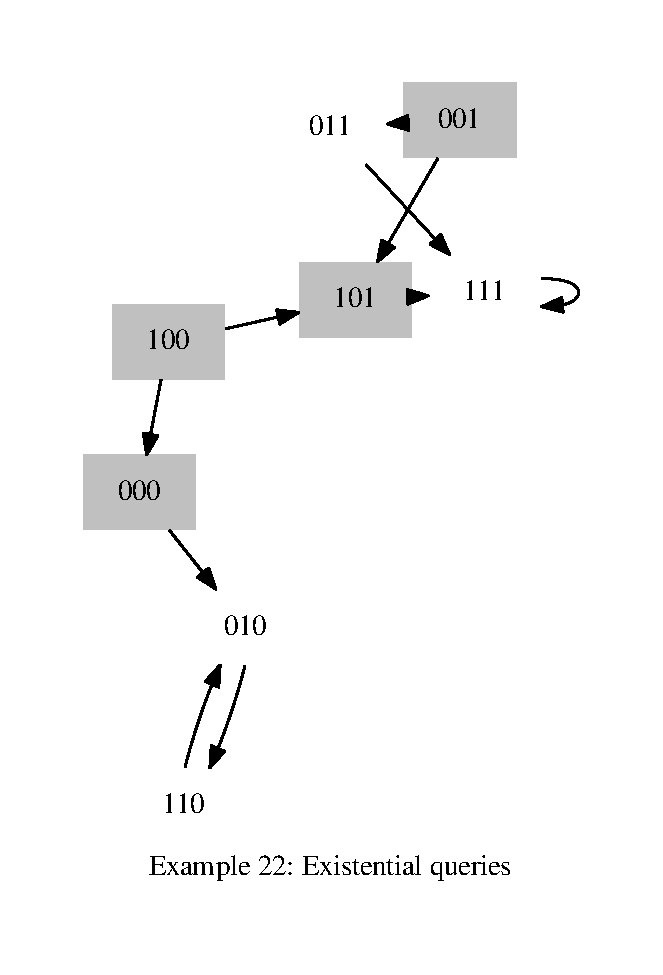
\includegraphics{figure22.pdf}}
\caption{The state transition graph \emph{``example22\_stg.pdf''} with initial states highlighted by gray rectangles.
The attractors are the steady state 111 and the cyclic attractor that consists of the states 010 and 110.}\label{Manual:figure22}\end{figure}

To decide the queries with CTL model checking we use the following encoding:

\begin{Verbatim}[commandchars=\\\{\}]
\PYG{g+gp}{\PYGZgt{}\PYGZgt{}\PYGZgt{} }\PYG{n}{init} \PYG{o}{=} \PYG{l+s}{\PYGZdq{}}\PYG{l+s}{INIT !x1}\PYG{l+s}{\PYGZdq{}}
\PYG{g+gp}{\PYGZgt{}\PYGZgt{}\PYGZgt{} }\PYG{n}{specQ1} \PYG{o}{=} \PYG{l+s}{\PYGZdq{}}\PYG{l+s}{CTLSPEC  EF(AG(x0\PYGZus{}STEADY))}\PYG{l+s}{\PYGZdq{}}
\PYG{g+gp}{\PYGZgt{}\PYGZgt{}\PYGZgt{} }\PYG{n}{specQ2} \PYG{o}{=} \PYG{l+s}{\PYGZdq{}}\PYG{l+s}{CTLSPEC !EF(AG(x0\PYGZus{}STEADY))}\PYG{l+s}{\PYGZdq{}}

\PYG{g+gp}{\PYGZgt{}\PYGZgt{}\PYGZgt{} }\PYG{n}{update} \PYG{o}{=} \PYG{l+s}{\PYGZdq{}}\PYG{l+s}{asynchronous}\PYG{l+s}{\PYGZdq{}}
\PYG{g+gp}{\PYGZgt{}\PYGZgt{}\PYGZgt{} }\PYG{n}{Q1} \PYG{o}{=} \PYG{n}{MC}\PYG{o}{.}\PYG{n}{check\PYGZus{}primes}\PYG{p}{(}\PYG{n}{primes}\PYG{p}{,} \PYG{n}{update}\PYG{p}{,} \PYG{n}{init}\PYG{p}{,} \PYG{n}{specQ1}\PYG{p}{)}
\PYG{g+gp}{\PYGZgt{}\PYGZgt{}\PYGZgt{} }\PYG{n}{Q1}
\PYG{g+go}{False}
\PYG{g+gp}{\PYGZgt{}\PYGZgt{}\PYGZgt{} }\PYG{n}{Q2} \PYG{o}{=} \PYG{o+ow}{not} \PYG{n}{MC}\PYG{o}{.}\PYG{n}{check\PYGZus{}primes}\PYG{p}{(}\PYG{n}{primes}\PYG{p}{,} \PYG{n}{update}\PYG{p}{,} \PYG{n}{init}\PYG{p}{,} \PYG{n}{specQ2}\PYG{p}{)}
\PYG{g+gp}{\PYGZgt{}\PYGZgt{}\PYGZgt{} }\PYG{n}{Q2}
\PYG{g+go}{True}
\end{Verbatim}

Note that \emph{specQ2} is exactly the negation of \emph{specQ1} and the result of checking \emph{specQ2} has to be negated to obtain the answer to Q2.

\begin{notice}{note}{Note:}
The queries \emph{specQ1} and \emph{specQ2} are both false although one is exactly the negation of the other.
In LTL and CTL model checking, a formula as well as its negation may be false \emph{simultaneously}.
For CTL, this is the case when some initial state satisfy the formula and some other initial state does not.
For LTL, this is the case when some admissible path satisfies the formula and some other path does not.
\end{notice}

Note also that since \emph{specQ2} is false we can ask {\hyperref[Installation:installation-nusmv]{\emph{NuSMV}}} to generate a counterexample, i.e.,
an initial state that does not satisfy \emph{specQ2}, i.e., a state that satisfies Q2.
Counterexamples of existential queries are therefore often also called \emph{witnesses}.

\begin{Verbatim}[commandchars=\\\{\}]
\PYG{g+gp}{\PYGZgt{}\PYGZgt{}\PYGZgt{} }\PYG{n}{notQ2}\PYG{p}{,} \PYG{n}{counterex} \PYG{o}{=} \PYG{n}{MC}\PYG{o}{.}\PYG{n}{check\PYGZus{}primes\PYGZus{}with\PYGZus{}counterexample}\PYG{p}{(}\PYG{n}{primes}\PYG{p}{,} \PYG{n}{update}\PYG{p}{,} \PYG{n}{init}\PYG{p}{,} \PYG{n}{specQ2}\PYG{p}{)}
\PYG{g+gp}{\PYGZgt{}\PYGZgt{}\PYGZgt{} }\PYG{n}{state} \PYG{o}{=} \PYG{n}{counterex}\PYG{p}{[}\PYG{l+m+mi}{0}\PYG{p}{]}
\PYG{g+gp}{\PYGZgt{}\PYGZgt{}\PYGZgt{} }\PYG{n}{STGs}\PYG{o}{.}\PYG{n}{state2str}\PYG{p}{(}\PYG{n}{state}\PYG{p}{)}
\PYG{g+go}{100}
\end{Verbatim}


\subsection{accepting states of CTL queries}
\label{Manual:accepting-states-of-ctl-queries}
Since Version 2.0 PyBoolnet supports model checking with so-called accepting states.
That is, PyBoolNet uses \href{https://github.com/hklarner/NuSMV-a}{NuSMV-a} to return a Boolean expression that represents all states that satisfy the CTL spec and another Boolean
expression that represents all initial states that satisfy the CTL spec.
The functionality of returning accepting states was implemented in \href{https://github.com/hklarner/NuSMV-a}{NuSMV-a}, an extension of \href{http://nusmv.fbk.eu}{NuSMV}.
To return the accepting states use the function \emph{check\_primes\_with\_acceptingstates} or {\hyperref[ModelChecking:check-smv-with-acceptingstates]{\emph{check\_smv\_with\_acceptingstates}}}.
It returns a tuple consisting of the answer and a dictionary with the following keys and values:
\begin{itemize}
\item {} 
\code{"INIT"}: \emph{str}, a factored formula representing the initial states

\item {} 
\code{"INIT\_SIZE"}: \emph{int}, the cardinality of the initial states

\item {} 
\code{"ACCEPTING"}: \emph{str}, a factored formula representing the accepting states

\item {} 
\code{"ACCEPTING\_SIZE"}: \emph{int}, the cardinality of the accepting states

\item {} 
\code{"INITACCEPTING"}: \emph{str}, a factored formula representing the initial and accepting states

\item {} 
\code{"INITACCEPTING\_SIZE"}: \emph{int}, the cardinality of the initial and accepting states

\end{itemize}

Consider the previous network as an example:

\begin{Verbatim}[commandchars=\\\{\}]
\PYG{g+gp}{\PYGZgt{}\PYGZgt{}\PYGZgt{} }\PYG{n}{bnet} \PYG{o}{=} \PYG{p}{[}\PYG{l+s}{\PYGZdq{}}\PYG{l+s}{x0,   !x0\PYGZam{}x1 \textbar{} x2}\PYG{l+s}{\PYGZdq{}}\PYG{p}{,}
\PYG{g+gp}{... }        \PYG{l+s}{\PYGZdq{}}\PYG{l+s}{x1,   !x0 \textbar{} x1 \textbar{} x2}\PYG{l+s}{\PYGZdq{}}\PYG{p}{,}
\PYG{g+gp}{... }        \PYG{l+s}{\PYGZdq{}}\PYG{l+s}{x2,   x0\PYGZam{}!x1 \textbar{} x2}\PYG{l+s}{\PYGZdq{}}\PYG{p}{]}
\PYG{g+gp}{\PYGZgt{}\PYGZgt{}\PYGZgt{} }\PYG{n}{bnet} \PYG{o}{=} \PYG{l+s}{\PYGZdq{}}\PYG{l+s+se}{\PYGZbs{}n}\PYG{l+s}{\PYGZdq{}}\PYG{o}{.}\PYG{n}{join}\PYG{p}{(}\PYG{n}{bnet}\PYG{p}{)}
\PYG{g+gp}{\PYGZgt{}\PYGZgt{}\PYGZgt{} }\PYG{n}{primes} \PYG{o}{=} \PYG{n}{FEX}\PYG{o}{.}\PYG{n}{bnet2primes}\PYG{p}{(}\PYG{n}{bnet}\PYG{p}{)}
\end{Verbatim}

We already know that the query with initial states \code{!x1} and the CTL spec \code{EF(AG(x0\_STEADY))} is false.
Using the function {\hyperref[ModelChecking:check-primes-with-counterexample]{\emph{check\_primes\_with\_counterexample}}} we found an initial state that does not satisfy the specification, i.e., 000.
The function {\hyperref[ModelChecking:check-primes-with-counterexample]{\emph{check\_primes\_with\_counterexample}}} can be used to get a complete picture of the intial states that satisfy the spec:

\begin{Verbatim}[commandchars=\\\{\}]
\PYG{g+gp}{\PYGZgt{}\PYGZgt{}\PYGZgt{} }\PYG{n}{update} \PYG{o}{=} \PYG{l+s}{\PYGZdq{}}\PYG{l+s}{asynchronous}\PYG{l+s}{\PYGZdq{}}
\PYG{g+gp}{\PYGZgt{}\PYGZgt{}\PYGZgt{} }\PYG{n}{init} \PYG{o}{=} \PYG{l+s}{\PYGZdq{}}\PYG{l+s}{INIT !x1}\PYG{l+s}{\PYGZdq{}}
\PYG{g+gp}{\PYGZgt{}\PYGZgt{}\PYGZgt{} }\PYG{n}{spec} \PYG{o}{=} \PYG{l+s}{\PYGZdq{}}\PYG{l+s}{CTLSPEC EF(AG(x0\PYGZus{}STEADY))}\PYG{l+s}{\PYGZdq{}}
\PYG{g+gp}{\PYGZgt{}\PYGZgt{}\PYGZgt{} }\PYG{n}{answer}\PYG{p}{,} \PYG{n}{accepting} \PYG{o}{=} \PYG{n}{MC}\PYG{o}{.}\PYG{n}{check\PYGZus{}primes\PYGZus{}with\PYGZus{}acceptingstates}\PYG{p}{(}\PYG{n}{primes}\PYG{p}{,} \PYG{n}{update}\PYG{p}{,} \PYG{n}{init}\PYG{p}{,} \PYG{n}{spec}\PYG{p}{)}
\PYG{g+gp}{\PYGZgt{}\PYGZgt{}\PYGZgt{} }\PYG{n}{accepting}\PYG{p}{[}\PYG{l+s}{\PYGZdq{}}\PYG{l+s}{INITACCEPTING}\PYG{l+s}{\PYGZdq{}}\PYG{p}{]}
\PYG{g+go}{\PYGZsq{}!(x0 \PYGZam{} (x1) \textbar{} !x0 \PYGZam{} (x1 \textbar{} !(x2)))\PYGZsq{}}
\end{Verbatim}

The result is a \emph{factored formula} that represents the exact set of states that satisfy the spec in NuSMV syntax so that it can be re-used for subsequent queries.
The number of initial and accepting states can be obtained by:

\begin{Verbatim}[commandchars=\\\{\}]
\PYG{g+gp}{\PYGZgt{}\PYGZgt{}\PYGZgt{} }\PYG{n}{accepting}\PYG{p}{[}\PYG{l+s}{\PYGZdq{}}\PYG{l+s}{INITACCEPTING\PYGZus{}SIZE}\PYG{l+s}{\PYGZdq{}}\PYG{p}{]}
\PYG{g+go}{3}
\end{Verbatim}

which explains why the query is false, since there are four initial states, i.e., one that does not satisfy the spec:

\begin{Verbatim}[commandchars=\\\{\}]
\PYG{g+gp}{\PYGZgt{}\PYGZgt{}\PYGZgt{} }\PYG{n}{accepting}\PYG{p}{[}\PYG{l+s}{\PYGZdq{}}\PYG{l+s}{INIT\PYGZus{}SIZE}\PYG{l+s}{\PYGZdq{}}\PYG{p}{]}
\PYG{g+go}{4}
\end{Verbatim}

It is also possible to obtain the complete set of states that satisfy the spec, i.e., including states that are not initial:

\begin{Verbatim}[commandchars=\\\{\}]
\PYG{g+gp}{\PYGZgt{}\PYGZgt{}\PYGZgt{} }\PYG{n}{accepting}\PYG{p}{[}\PYG{l+s}{\PYGZdq{}}\PYG{l+s}{ACCEPTING}\PYG{l+s}{\PYGZdq{}}\PYG{p}{]}
\PYG{g+go}{\PYGZsq{}x0 \PYGZam{} ((x2) \textbar{} !x1) \textbar{} !x0 \PYGZam{} (x2)\PYGZsq{}}
\end{Verbatim}

The size of this set tells us that there are two states outside of the initial one that also satisfy the spec:

\begin{Verbatim}[commandchars=\\\{\}]
\PYG{g+gp}{\PYGZgt{}\PYGZgt{}\PYGZgt{} }\PYG{n}{accepting}\PYG{p}{[}\PYG{l+s}{\PYGZdq{}}\PYG{l+s}{ACCEPTING\PYGZus{}SIZE}\PYG{l+s}{\PYGZdq{}}\PYG{p}{]}
\PYG{g+go}{5}
\end{Verbatim}

Note that \emph{PyBoolNet 2.11} does not currently support the manipulation of Boolean expression. They may however be used in subsequent queries.
For example, we may query whether all initial states that satisfy the original spec also satisfy the property \code{EF(STEADYSTATE)}:

\begin{Verbatim}[commandchars=\\\{\}]
\PYG{g+gp}{\PYGZgt{}\PYGZgt{}\PYGZgt{} }\PYG{n}{prop} \PYG{o}{=} \PYG{n}{accepting}\PYG{p}{[}\PYG{l+s}{\PYGZdq{}}\PYG{l+s}{INITACCEPTING}\PYG{l+s}{\PYGZdq{}}\PYG{p}{]}
\PYG{g+gp}{\PYGZgt{}\PYGZgt{}\PYGZgt{} }\PYG{n}{init} \PYG{o}{=} \PYG{l+s}{\PYGZdq{}}\PYG{l+s}{INIT }\PYG{l+s+si}{\PYGZpc{}s}\PYG{l+s}{\PYGZdq{}}\PYG{o}{\PYGZpc{}}\PYG{n}{prop}
\PYG{g+gp}{\PYGZgt{}\PYGZgt{}\PYGZgt{} }\PYG{n}{spec} \PYG{o}{=} \PYG{l+s}{\PYGZdq{}}\PYG{l+s}{CTLSPEC EF(STEADYSTATE)}\PYG{l+s}{\PYGZdq{}}
\PYG{g+gp}{\PYGZgt{}\PYGZgt{}\PYGZgt{} }\PYG{n}{MC}\PYG{o}{.}\PYG{n}{check\PYGZus{}primes}\PYG{p}{(}\PYG{n}{primes}\PYG{p}{,} \PYG{n}{update}\PYG{p}{,} \PYG{n}{init}\PYG{p}{,} \PYG{n}{spec}\PYG{p}{)}
\PYG{g+go}{True}
\end{Verbatim}

You can use the function {\hyperref[StateTransitionGraphs:list-states-referenced-by-proposition]{\emph{list\_states\_referenced\_by\_proposition}}} to enumerate all states that are referenced by a propositional formula:

\begin{Verbatim}[commandchars=\\\{\}]
\PYG{g+gp}{\PYGZgt{}\PYGZgt{}\PYGZgt{} }\PYG{k}{for} \PYG{n}{x} \PYG{o+ow}{in} \PYG{n}{STGs}\PYG{o}{.}\PYG{n}{list\PYGZus{}states\PYGZus{}referenced\PYGZus{}by\PYGZus{}proposition}\PYG{p}{(}\PYG{n}{primes}\PYG{p}{,} \PYG{n}{prop}\PYG{p}{)}\PYG{p}{:} \PYG{k}{print} \PYG{n}{x}
\PYG{g+go}{001}
\PYG{g+go}{101}
\PYG{g+go}{100}
\end{Verbatim}


\section{Computing Trap Spaces}
\label{Manual:computing-trap-spaces}
Maximal, Minimal and All Trap Spaces
The term \emph{trap space} merges the notions ``subspace'' and ``trap set''.
Hence, once a trajectory enters a trap space it can not escape.
Trap spaces have a number of interesting properties: they are independent of the update strategy, i.e.,
they are identical for all state transition graphs, they satisfy a partial order defined by set inclusion of the respective states contained in them
and they can be computed efficiently for networks with hundreds of components.
Intuitively, trap spaces can be seen as generalizations of steady states (note that steady states have the same three properties).
For a formal introduction, an algorithm for computing trap spaces and a benchmark see {\hyperref[Bibliography:klarner2015trap]{\emph{Klarner2015(a)}}}.

\emph{PyBoolNet 2.11} uses the module {\hyperref[TrapSpaces:trapspaces]{\emph{TrapSpaces}}} and the function {\hyperref[TrapSpaces:trap-spaces]{\emph{trap\_spaces}}} to compute trap spaces.
As an example, consider the following network which has five trap spaces:

\begin{Verbatim}[commandchars=\\\{\}]
\PYG{g+gp}{\PYGZgt{}\PYGZgt{}\PYGZgt{} }\PYG{k+kn}{from} \PYG{n+nn}{PyBoolNet} \PYG{k+kn}{import} \PYG{n}{TrapSpaces} \PYG{k}{as} \PYG{n}{TS}
\PYG{g+gp}{\PYGZgt{}\PYGZgt{}\PYGZgt{} }\PYG{n}{bnet} \PYG{o}{=} \PYG{p}{[}\PYG{l+s}{\PYGZdq{}}\PYG{l+s}{x, !x \textbar{} y \textbar{} z}\PYG{l+s}{\PYGZdq{}}\PYG{p}{,}
\PYG{g+gp}{... }        \PYG{l+s}{\PYGZdq{}}\PYG{l+s}{y, !x\PYGZam{}z \textbar{} y\PYGZam{}!z}\PYG{l+s}{\PYGZdq{}}\PYG{p}{,}
\PYG{g+gp}{... }        \PYG{l+s}{\PYGZdq{}}\PYG{l+s}{z, x\PYGZam{}y \textbar{} z}\PYG{l+s}{\PYGZdq{}}\PYG{p}{]}
\PYG{g+gp}{\PYGZgt{}\PYGZgt{}\PYGZgt{} }\PYG{n}{bnet} \PYG{o}{=} \PYG{l+s}{\PYGZdq{}}\PYG{l+s+se}{\PYGZbs{}n}\PYG{l+s}{\PYGZdq{}}\PYG{o}{.}\PYG{n}{join}\PYG{p}{(}\PYG{n}{bnet}\PYG{p}{)}
\PYG{g+gp}{\PYGZgt{}\PYGZgt{}\PYGZgt{} }\PYG{n}{primes} \PYG{o}{=} \PYG{n}{FEX}\PYG{o}{.}\PYG{n}{bnet2primes}\PYG{p}{(}\PYG{n}{bnet}\PYG{p}{)}
\PYG{g+gp}{\PYGZgt{}\PYGZgt{}\PYGZgt{} }\PYG{n}{tspaces} \PYG{o}{=} \PYG{n}{TS}\PYG{o}{.}\PYG{n}{trap\PYGZus{}spaces}\PYG{p}{(}\PYG{n}{primes}\PYG{p}{,} \PYG{l+s}{\PYGZdq{}}\PYG{l+s}{all}\PYG{l+s}{\PYGZdq{}}\PYG{p}{)}
\PYG{g+gp}{\PYGZgt{}\PYGZgt{}\PYGZgt{} }\PYG{k}{print} \PYG{l+s}{\PYGZdq{}}\PYG{l+s}{, }\PYG{l+s}{\PYGZdq{}}\PYG{o}{.}\PYG{n}{join}\PYG{p}{(}\PYG{n}{STGs}\PYG{o}{.}\PYG{n}{subspace2str}\PYG{p}{(}\PYG{n}{primes}\PYG{p}{,} \PYG{n}{x}\PYG{p}{)} \PYG{k}{for} \PYG{n}{x} \PYG{o+ow}{in} \PYG{n}{tspaces}\PYG{p}{)}
\PYG{g+go}{\PYGZhy{}\PYGZhy{}\PYGZhy{}, \PYGZhy{}\PYGZhy{}1, 1\PYGZhy{}1, \PYGZhy{}00, 101}
\end{Verbatim}

The trap space \code{-{-}-}, i.e., the full state space, is also called the trivial trap space.
\code{101} is a steady state and there are three more trap spaces, \code{-{-}1}, \code{1-1} and \code{-00}.
Note that some trap spaces are comparable using subset inclusion, i.e.,
\code{1-1} \textless{} \code{-{-}1} because the two states contained in \code{1-1} are also contained in \code{-{-}1},
while others are not comparable, for example \code{-{-}1} and \code{-00}.

The trap spaces are illustrated in {\hyperref[Manual:figure23]{\emph{the figure below}}} using the subspaces style:

\begin{Verbatim}[commandchars=\\\{\}]
\PYG{g+gp}{\PYGZgt{}\PYGZgt{}\PYGZgt{} }\PYG{n}{stg} \PYG{o}{=} \PYG{n}{STGs}\PYG{o}{.}\PYG{n}{primes2stg}\PYG{p}{(}\PYG{n}{primes}\PYG{p}{,} \PYG{l+s}{\PYGZdq{}}\PYG{l+s}{asynchronous}\PYG{l+s}{\PYGZdq{}}\PYG{p}{)}
\PYG{g+gp}{\PYGZgt{}\PYGZgt{}\PYGZgt{} }\PYG{n}{STGs}\PYG{o}{.}\PYG{n}{add\PYGZus{}style\PYGZus{}subspaces}\PYG{p}{(}\PYG{n}{primes}\PYG{p}{,} \PYG{n}{stg}\PYG{p}{,} \PYG{n}{tspaces}\PYG{p}{)}
\PYG{g+gp}{\PYGZgt{}\PYGZgt{}\PYGZgt{} }\PYG{n}{stg}\PYG{o}{.}\PYG{n}{graph}\PYG{p}{[}\PYG{l+s}{\PYGZdq{}}\PYG{l+s}{label}\PYG{l+s}{\PYGZdq{}}\PYG{p}{]} \PYG{o}{=} \PYG{l+s}{\PYGZdq{}}\PYG{l+s}{Example 23: All trap spaces}\PYG{l+s}{\PYGZdq{}}
\PYG{g+gp}{\PYGZgt{}\PYGZgt{}\PYGZgt{} }\PYG{n}{STGs}\PYG{o}{.}\PYG{n}{stg2image}\PYG{p}{(}\PYG{n}{stg}\PYG{p}{,} \PYG{l+s}{\PYGZdq{}}\PYG{l+s}{example23\PYGZus{}stg.pdf}\PYG{l+s}{\PYGZdq{}}\PYG{p}{)}
\end{Verbatim}
\begin{figure}[htbp]
\centering
\capstart

\scalebox{0.600000}{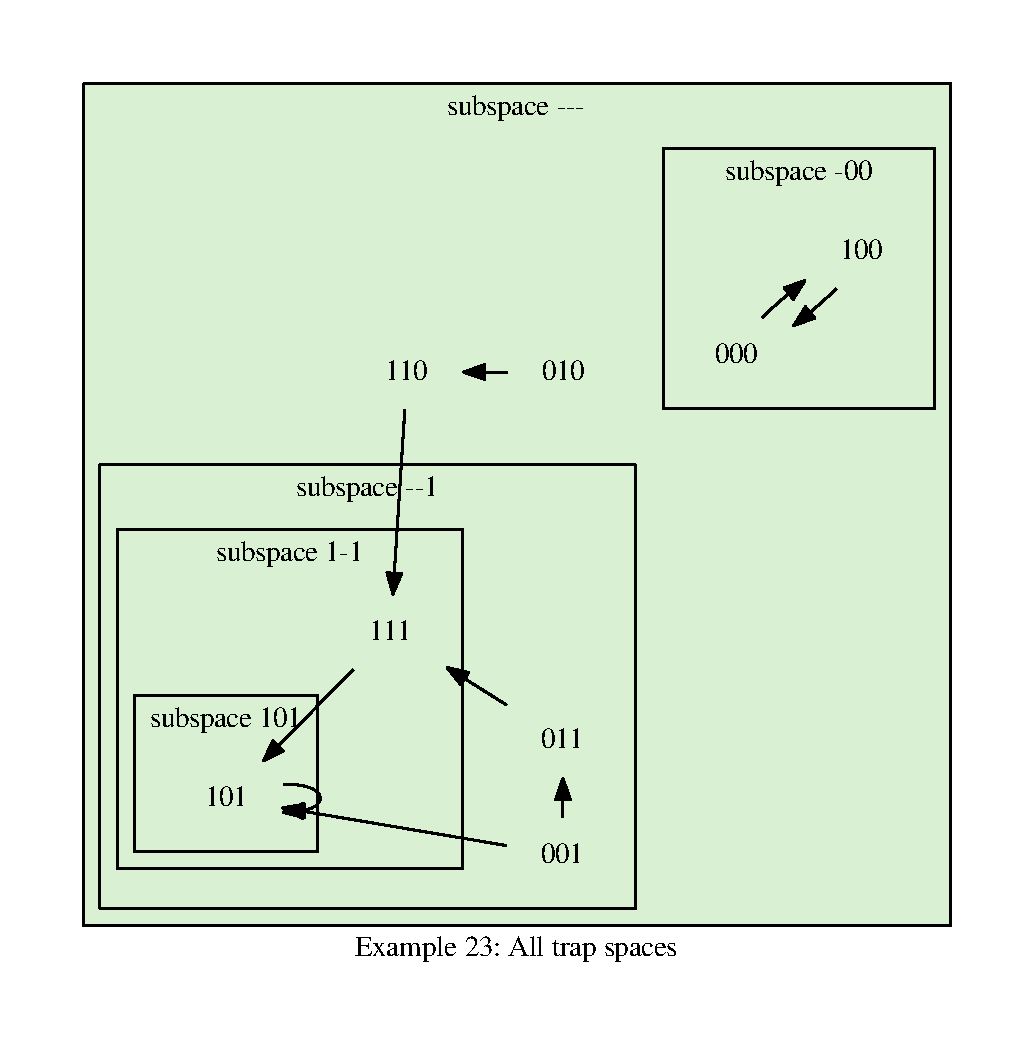
\includegraphics{figure23.pdf}}
\caption{The state transition graph \emph{``example23\_stg.pdf''} with every trap space highlighted by its own subgraph.}\label{Manual:figure23}\end{figure}

The number of all trap spaces of a network can be very large and one is often only interested in the subset of minimal or maximal trap spaces.
These can also be computed using {\hyperref[TrapSpaces:trap-spaces]{\emph{trap\_spaces}}} by passing \emph{``min''} or \emph{``max''} instead of the previously used value \emph{``all''} for the second parameter:

\begin{Verbatim}[commandchars=\\\{\}]
\PYG{g+gp}{\PYGZgt{}\PYGZgt{}\PYGZgt{} }\PYG{n}{mintspaces} \PYG{o}{=} \PYG{n}{TS}\PYG{o}{.}\PYG{n}{trap\PYGZus{}spaces}\PYG{p}{(}\PYG{n}{primes}\PYG{p}{,} \PYG{l+s}{\PYGZdq{}}\PYG{l+s}{min}\PYG{l+s}{\PYGZdq{}}\PYG{p}{)}
\PYG{g+gp}{\PYGZgt{}\PYGZgt{}\PYGZgt{} }\PYG{k}{for} \PYG{n}{x} \PYG{o+ow}{in} \PYG{n}{mintspaces}\PYG{p}{:}
\PYG{g+gp}{... }    \PYG{n}{sub} \PYG{o}{=} \PYG{p}{(}\PYG{n}{x}\PYG{p}{,}\PYG{p}{\PYGZob{}}\PYG{l+s}{\PYGZdq{}}\PYG{l+s}{fillcolor}\PYG{l+s}{\PYGZdq{}}\PYG{p}{:}\PYG{l+s}{\PYGZdq{}}\PYG{l+s}{salmon}\PYG{l+s}{\PYGZdq{}}\PYG{p}{\PYGZcb{}}\PYG{p}{)}
\PYG{g+gp}{... }    \PYG{n}{STGs}\PYG{o}{.}\PYG{n}{add\PYGZus{}style\PYGZus{}subspaces}\PYG{p}{(}\PYG{n}{primes}\PYG{p}{,} \PYG{n}{stg}\PYG{p}{,} \PYG{p}{[}\PYG{n}{sub}\PYG{p}{]}\PYG{p}{)}
\PYG{g+gp}{\PYGZgt{}\PYGZgt{}\PYGZgt{} }\PYG{n}{maxtspaces} \PYG{o}{=} \PYG{n}{TS}\PYG{o}{.}\PYG{n}{trap\PYGZus{}spaces}\PYG{p}{(}\PYG{n}{primes}\PYG{p}{,} \PYG{l+s}{\PYGZdq{}}\PYG{l+s}{max}\PYG{l+s}{\PYGZdq{}}\PYG{p}{)}
\PYG{g+gp}{\PYGZgt{}\PYGZgt{}\PYGZgt{} }\PYG{k}{for} \PYG{n}{x} \PYG{o+ow}{in} \PYG{n}{maxtspaces}\PYG{p}{:}
\PYG{g+gp}{... }    \PYG{k}{if} \PYG{n}{x} \PYG{o+ow}{in} \PYG{n}{mintspaces}\PYG{p}{:}
\PYG{g+gp}{... }        \PYG{n}{sub} \PYG{o}{=} \PYG{p}{(}\PYG{n}{x}\PYG{p}{,}\PYG{p}{\PYGZob{}}\PYG{l+s}{\PYGZdq{}}\PYG{l+s}{fillcolor}\PYG{l+s}{\PYGZdq{}}\PYG{p}{:}\PYG{l+s}{\PYGZdq{}}\PYG{l+s}{lightyellow}\PYG{l+s}{\PYGZdq{}}\PYG{p}{\PYGZcb{}}\PYG{p}{)}
\PYG{g+gp}{... }        \PYG{n}{STGs}\PYG{o}{.}\PYG{n}{add\PYGZus{}style\PYGZus{}subspaces}\PYG{p}{(}\PYG{n}{primes}\PYG{p}{,} \PYG{n}{stg}\PYG{p}{,} \PYG{p}{[}\PYG{n}{sub}\PYG{p}{]}\PYG{p}{)}
\PYG{g+gp}{... }    \PYG{k}{else}\PYG{p}{:}
\PYG{g+gp}{... }        \PYG{n}{sub} \PYG{o}{=} \PYG{p}{(}\PYG{n}{x}\PYG{p}{,}\PYG{p}{\PYGZob{}}\PYG{l+s}{\PYGZdq{}}\PYG{l+s}{fillcolor}\PYG{l+s}{\PYGZdq{}}\PYG{p}{:}\PYG{l+s}{\PYGZdq{}}\PYG{l+s}{lightblue}\PYG{l+s}{\PYGZdq{}}\PYG{p}{\PYGZcb{}}\PYG{p}{)}
\PYG{g+gp}{... }        \PYG{n}{STGs}\PYG{o}{.}\PYG{n}{add\PYGZus{}style\PYGZus{}subspaces}\PYG{p}{(}\PYG{n}{primes}\PYG{p}{,} \PYG{n}{stg}\PYG{p}{,} \PYG{p}{[}\PYG{n}{sub}\PYG{p}{]}\PYG{p}{)}
\PYG{g+gp}{\PYGZgt{}\PYGZgt{}\PYGZgt{} }\PYG{n}{stg}\PYG{o}{.}\PYG{n}{graph}\PYG{p}{[}\PYG{l+s}{\PYGZdq{}}\PYG{l+s}{label}\PYG{l+s}{\PYGZdq{}}\PYG{p}{]} \PYG{o}{=} \PYG{l+s}{\PYGZdq{}}\PYG{l+s}{Example 24: Minimal and maximal trap spaces}\PYG{l+s}{\PYGZdq{}}
\PYG{g+gp}{\PYGZgt{}\PYGZgt{}\PYGZgt{} }\PYG{n}{STGs}\PYG{o}{.}\PYG{n}{stg2image}\PYG{p}{(}\PYG{n}{stg}\PYG{p}{,} \PYG{l+s}{\PYGZdq{}}\PYG{l+s}{example24\PYGZus{}stg.pdf}\PYG{l+s}{\PYGZdq{}}\PYG{p}{)}
\end{Verbatim}

The result is shown in {\hyperref[Manual:figure24]{\emph{the figure below}}} in which \code{-00} is minimal and maximal (yellow),
\code{-{-}1} is maximal (blue), \code{1-1} is neither maximal nor minimal (green), and \code{101} is minimal (red).
\begin{figure}[htbp]
\centering
\capstart

\scalebox{0.600000}{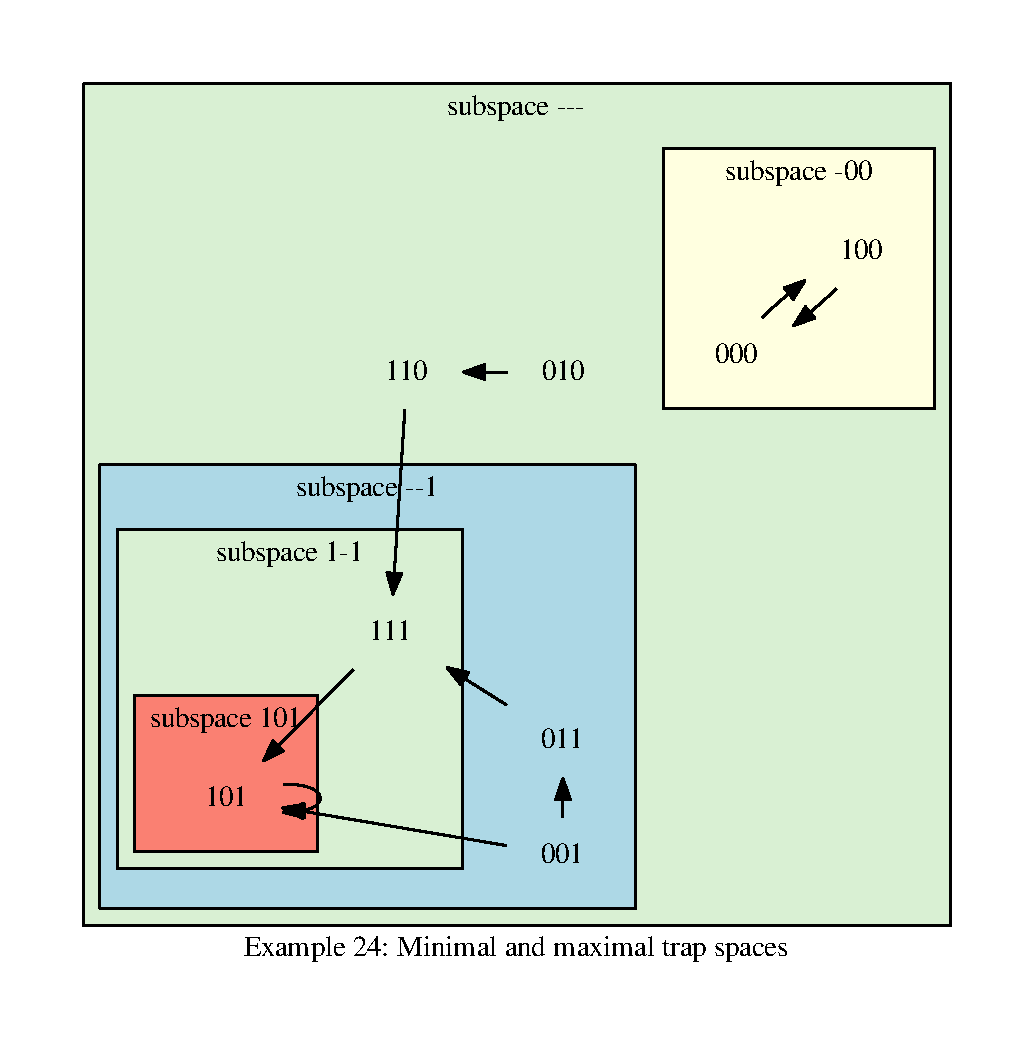
\includegraphics{figure24.pdf}}
\caption{The state transition graph \emph{``example24\_stg.pdf''} with minimal trap spaces in red, maximal trap spaces in blue,
trap spaces that are minimal and maximal at the same time in yellow and the remaining trap spaces in green.}\label{Manual:figure24}\end{figure}

\begin{notice}{note}{Note:}
It is possible that two non-minimal trap spaces intersect in which case the intersection is again a trap space.
Since {\hyperref[Installation:installation-graphviz]{\emph{Graphviz}}} can not draw intersecting subgraphs it is therefore not always possible to draw all trap spaces.
Minimal trap spaces on the other hand, can not intersect and can always be drawn in the same STG.
\end{notice}


\section{Attractors}
\label{Manual:attractors}

\subsection{attractor detection}
\label{Manual:attractor-detection}
Attractors capture the long-term activities of the components of Boolean networks.
Two different types of attractors are possible: either all activities stabilize at some values and the network enters a steady state or at least one component shows sustained oscillations and the network enters a cyclic attractor.
Formally, attractors are defined as the inclusion-wise minimal trap sets of a given STG which is equivalent to the so-called terminal SCCs of the state transition graph.
One approach to computing the attractors is to use Tarjan's algorithm for computing the SCCs of a directed graph, see {\hyperref[Bibliography:tarjan1972]{\emph{Tarjan1972}}} and then to select those SCCs that are terminal, i.e., those for which there is no path to another SCC.
This approach is implemented in the function {\hyperref[AttractorDetection:compute-attractors-tarjan]{\emph{compute\_attractors\_tarjan}}}.
As an example for computing attractors with this algorithm consider the following network and its asynchronous STG which is given in {\hyperref[Manual:figure25]{\emph{the figure below}}}:

\begin{Verbatim}[commandchars=\\\{\}]
\PYG{g+gp}{\PYGZgt{}\PYGZgt{}\PYGZgt{} }\PYG{k+kn}{import} \PYG{n+nn}{AttractorDetection} \PYG{k+kn}{as} \PYG{n+nn}{AD}
\PYG{g+gp}{\PYGZgt{}\PYGZgt{}\PYGZgt{} }\PYG{n}{bnet} \PYG{o}{=} \PYG{p}{[}\PYG{l+s}{\PYGZdq{}}\PYG{l+s}{v1, !v1 \textbar{} v3}\PYG{l+s}{\PYGZdq{}}\PYG{p}{,}
\PYG{g+gp}{... }        \PYG{l+s}{\PYGZdq{}}\PYG{l+s}{v2, !v1 \textbar{} v2\PYGZam{}!v3}\PYG{l+s}{\PYGZdq{}}\PYG{p}{,}
\PYG{g+gp}{... }        \PYG{l+s}{\PYGZdq{}}\PYG{l+s}{v3, !v2}\PYG{l+s}{\PYGZdq{}}\PYG{p}{]}
\PYG{g+gp}{\PYGZgt{}\PYGZgt{}\PYGZgt{} }\PYG{n}{bnet} \PYG{o}{=} \PYG{l+s}{\PYGZdq{}}\PYG{l+s+se}{\PYGZbs{}n}\PYG{l+s}{\PYGZdq{}}\PYG{o}{.}\PYG{n}{join}\PYG{p}{(}\PYG{n}{bnet}\PYG{p}{)}
\PYG{g+gp}{\PYGZgt{}\PYGZgt{}\PYGZgt{} }\PYG{n}{primes} \PYG{o}{=} \PYG{n}{FEX}\PYG{o}{.}\PYG{n}{bnet2primes}\PYG{p}{(}\PYG{n}{bnet}\PYG{p}{)}
\PYG{g+gp}{\PYGZgt{}\PYGZgt{}\PYGZgt{} }\PYG{n}{stg} \PYG{o}{=} \PYG{n}{STGs}\PYG{o}{.}\PYG{n}{primes2stg}\PYG{p}{(}\PYG{n}{primes}\PYG{p}{,} \PYG{l+s}{\PYGZdq{}}\PYG{l+s}{asynchronous}\PYG{l+s}{\PYGZdq{}}\PYG{p}{)}
\PYG{g+gp}{\PYGZgt{}\PYGZgt{}\PYGZgt{} }\PYG{n}{STGs}\PYG{o}{.}\PYG{n}{add\PYGZus{}style\PYGZus{}sccs}\PYG{p}{(}\PYG{n}{stg}\PYG{p}{)}
\PYG{g+gp}{\PYGZgt{}\PYGZgt{}\PYGZgt{} }\PYG{n}{stg}\PYG{o}{.}\PYG{n}{graph}\PYG{p}{[}\PYG{l+s}{\PYGZdq{}}\PYG{l+s}{label}\PYG{l+s}{\PYGZdq{}}\PYG{p}{]} \PYG{o}{=} \PYG{l+s}{\PYGZdq{}}\PYG{l+s}{Example 25: A network with a cyclic attractor and a steady state.}\PYG{l+s}{\PYGZdq{}}
\PYG{g+gp}{\PYGZgt{}\PYGZgt{}\PYGZgt{} }\PYG{n}{STGs}\PYG{o}{.}\PYG{n}{stg2image}\PYG{p}{(}\PYG{n}{stg}\PYG{p}{,} \PYG{l+s}{\PYGZdq{}}\PYG{l+s}{example25\PYGZus{}stg.pdf}\PYG{l+s}{\PYGZdq{}}\PYG{p}{)}
\PYG{g+gp}{\PYGZgt{}\PYGZgt{}\PYGZgt{} }\PYG{n}{attractors} \PYG{o}{=} \PYG{n}{AD}\PYG{o}{.}\PYG{n}{compute\PYGZus{}attractors\PYGZus{}tarjan}\PYG{p}{(}\PYG{n}{stg}\PYG{p}{)}
\PYG{g+gp}{\PYGZgt{}\PYGZgt{}\PYGZgt{} }\PYG{n+nb}{len}\PYG{p}{(}\PYG{n}{attractors}\PYG{p}{)}
\PYG{g+go}{2}
\PYG{g+gp}{\PYGZgt{}\PYGZgt{}\PYGZgt{} }\PYG{k}{for} \PYG{n}{A} \PYG{o+ow}{in} \PYG{n}{attractors}\PYG{p}{:}
\PYG{g+gp}{... }    \PYG{k}{print} \PYG{p}{[}\PYG{n}{STGs}\PYG{o}{.}\PYG{n}{state2str}\PYG{p}{(}\PYG{n}{x}\PYG{p}{)} \PYG{k}{for} \PYG{n}{x} \PYG{o+ow}{in} \PYG{n}{A}\PYG{p}{]}
\PYG{g+go}{[\PYGZsq{}101\PYGZsq{}]}
\PYG{g+go}{[\PYGZsq{}010\PYGZsq{}, \PYGZsq{}110\PYGZsq{}]}
\end{Verbatim}
\begin{figure}[htbp]
\centering
\capstart

\scalebox{0.600000}{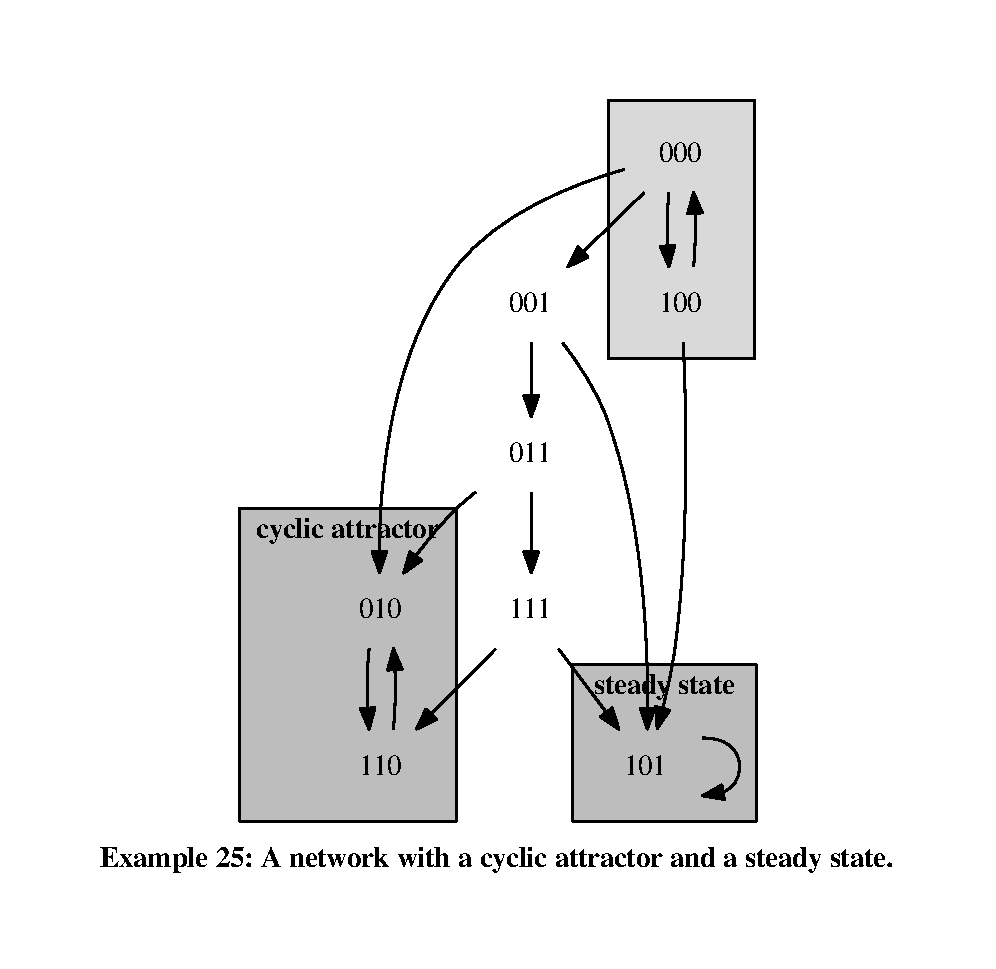
\includegraphics{figure25.pdf}}
\caption{The asynchronous STG \emph{``example25\_stg.pdf''} of a network with a steady state and a cyclic attractor.}\label{Manual:figure25}\end{figure}

Due to the state space explosion problem, the approach of computing the terminal SCCs by explicitly
constructing the underlying STG as a digraphis limited to networks with less than 15\textasciitilde{}20 components.

There are algorithms for larger networks, but the ``best'' algorithm for solving the detection problem will depend on the chosen update strategy.
For synchronous STGs we suggest to use an approach that was suggested
by {\hyperref[Bibliography:dubrova2011]{\emph{Dubrova2011}}} and involves a SAT solver and bounded LTL model checking.
It has been implemented as a tool called \emph{bns} which is available at \href{https://people.kth.se/~dubrova/bns.html}{https://people.kth.se/\textasciitilde{}dubrova/bns.html}.

\begin{notice}{note}{Note:}
Boolean networks can be converted into \emph{bns} file format with {\hyperref[FileExchange:primes2bns]{\emph{primes2bns}}}.
\end{notice}

\begin{notice}{note}{Note:}
Whereas the steady states of the synchronous and asynchronous STGs are identical,
the number and composition of cyclic attractors depends, in general, on the chosen update strategy.
\end{notice}

A fairly efficient approach to detecting at least some attractors or larger networks is mentioned in {\hyperref[Bibliography:klarner2015trap]{\emph{Klarner2015(a)}}}
and based on the idea of generating a random walk in the STG, starting from some initial state,
and then testing with CTL model checking whether the final state is indeed part of an attractor.
This approach is based on the observation that, in practice, a random walk will quickly reach states that belong to an attractor.
It is implemented in the function {\hyperref[AttractorDetection:find-attractor-state-by-randomwalk-and-ctl]{\emph{find\_attractor\_state\_by\_randomwalk\_and\_ctl}}}:

\begin{Verbatim}[commandchars=\\\{\}]
\PYG{g+gp}{\PYGZgt{}\PYGZgt{}\PYGZgt{} }\PYG{n}{state} \PYG{o}{=} \PYG{n}{AD}\PYG{o}{.}\PYG{n}{find\PYGZus{}attractor\PYGZus{}state\PYGZus{}by\PYGZus{}randomwalk\PYGZus{}and\PYGZus{}ctl}\PYG{p}{(}\PYG{n}{primes}\PYG{p}{,} \PYG{l+s}{\PYGZdq{}}\PYG{l+s}{asynchronous}\PYG{l+s}{\PYGZdq{}}\PYG{p}{)}
\PYG{g+gp}{\PYGZgt{}\PYGZgt{}\PYGZgt{} }\PYG{n}{STGs}\PYG{o}{.}\PYG{n}{state2str}\PYG{p}{(}\PYG{n}{state}\PYG{p}{)}
\PYG{g+go}{110}
\end{Verbatim}

The function takes three optional parameters: \emph{InitialState} which allows to specify a subspace from which to sample the initial state,
\emph{Length} which is an integer that specifies the number of transitions for the generation of the random walk,
and \emph{Attempts} which is the maximal number of random walks that are generated if each time the last state does not belong to an attractor.
Though unlikely, it is possible that the function will not find an attractor in which case it will raise an exception.
Hence, {\hyperref[AttractorDetection:find-attractor-state-by-randomwalk-and-ctl]{\emph{find\_attractor\_state\_by\_randomwalk\_and\_ctl}}} should always be encapsulated in a \emph{Try-Except} block:

\begin{Verbatim}[commandchars=\\\{\}]
\PYG{g+gp}{\PYGZgt{}\PYGZgt{}\PYGZgt{} }\PYG{k}{try}\PYG{p}{:}
\PYG{g+gp}{... }    \PYG{n}{state} \PYG{o}{=} \PYG{n}{AD}\PYG{o}{.}\PYG{n}{find\PYGZus{}attractor\PYGZus{}state\PYGZus{}by\PYGZus{}randomwalk\PYGZus{}and\PYGZus{}ctl}\PYG{p}{(}\PYG{n}{primes}\PYG{p}{,} \PYG{l+s}{\PYGZdq{}}\PYG{l+s}{asynchronous}\PYG{l+s}{\PYGZdq{}}\PYG{p}{)}
\PYG{g+gp}{... }    \PYG{k}{print} \PYG{n}{STGs}\PYG{o}{.}\PYG{n}{state2str}\PYG{p}{(}\PYG{n}{state}\PYG{p}{)}
\PYG{g+gp}{... }\PYG{k}{except}\PYG{p}{:}
\PYG{g+gp}{... }    \PYG{k}{print} \PYG{l+s}{\PYGZdq{}}\PYG{l+s}{did not find an attractor. try increasing the length or attempts parameters}\PYG{l+s}{\PYGZdq{}}
\end{Verbatim}


\subsection{attractor basins}
\label{Manual:attractor-basins}
The module {\hyperref[AttractorBasins:attractorbasins]{\emph{AttractorBasins}}} contains functions for constructing diagrams that illustrate the basins of attraction of a given STG.
In non-deterministic STGs there are usually states from which more than one attractor is reachable.
But, not every combination of attractors has states that can reach exactly that subset of attractors.
The function {\hyperref[AttractorBasins:basins-diagram]{\emph{basins\_diagram}}} checks for each possible combination of attractors whether the set of corresponding basin states is empty or not.
If there are states a basin node is created.
An edge between basin nodes indicates the existence of a transition between two states of the respective sets of states.
The nodes of a basin diagram have the following attributes:
\begin{itemize}
\item {} 
\code{"formula"} (str), the factored formula representing the states in that basin

\item {} 
\code{"size"} (int), the number of states in that basin

\item {} 
\code{"attractors"} (list), the list of attractors that define that basin (represented by individual states or subspaces)

\end{itemize}

The edges of a basin diagram have the following attributes:
\begin{itemize}
\item {} 
\code{"finally\_formula"} (str), the factored formula that represents the states that can reach a state that can make the transition

\item {} 
\code{"finally\_size"} (int), the number of such states

\end{itemize}

Basin diagrams can be visualized with the function {\hyperref[AttractorBasins:diagram2image]{\emph{diagram2image}}}.
The function takes the primes, diagram and file name of the image as parameters.
In addition you may specify \emph{FnameATTRACTORS} if you want a separate file for the specification of the attractors.
Otherwise they are included in the diagram image.
Two parameters for styling the diagram are provided.
\emph{StyleInputs} highlight the basin nodes that belong to the same input combination and \emph{StyleAdvanced} modifies the node and edge styles to
highlight nodes and transition that are \emph{homogeneous}. For details see the upcoming publication {\hyperref[Bibliography:klarner2016basins]{\emph{Klarner2016}}}.

Consider the following example:

\begin{Verbatim}[commandchars=\\\{\}]
\PYG{g+gp}{\PYGZgt{}\PYGZgt{}\PYGZgt{} }\PYG{n}{primes} \PYG{o}{=} \PYG{n}{REPO}\PYG{o}{.}\PYG{n}{get\PYGZus{}primes}\PYG{p}{(}\PYG{l+s}{\PYGZdq{}}\PYG{l+s}{arellano\PYGZus{}rootstem}\PYG{l+s}{\PYGZdq{}}\PYG{p}{)}
\PYG{g+gp}{\PYGZgt{}\PYGZgt{}\PYGZgt{} }\PYG{n}{diagram} \PYG{o}{=} \PYG{n}{AB}\PYG{o}{.}\PYG{n}{basins\PYGZus{}diagram}\PYG{p}{(}\PYG{n}{primes}\PYG{p}{,} \PYG{l+s}{\PYGZdq{}}\PYG{l+s}{asynchronous}\PYG{l+s}{\PYGZdq{}}\PYG{p}{)}
\PYG{g+gp}{\PYGZgt{}\PYGZgt{}\PYGZgt{} }\PYG{n}{AB}\PYG{o}{.}\PYG{n}{diagram2image}\PYG{p}{(}\PYG{n}{primes}\PYG{p}{,} \PYG{n}{diagram}\PYG{p}{,} \PYG{l+s}{\PYGZdq{}}\PYG{l+s}{diagram.pdf}\PYG{l+s}{\PYGZdq{}}\PYG{p}{)}
\end{Verbatim}

The output is given in \emph{the figure below}.
It uses the following convention: basin nodes that belong to the same input combination are grouped as light green subgraphs.
The fillcolor of a basin node reflects the proportion of states that belong to it: the darker the more states.
Nodes are labeled by the attractors they can reach which are enumerated by A0, A1, etc.
Cyclic attractros are represented by minimal trap spaces.

Note that the function {\hyperref[AttractorBasins:basins-diagram]{\emph{basins\_diagram}}} either requires a list of states representing attractors (given via the parameter \emph{Attractors}),
or it will compute the minimal trap spaces and \emph{assume} that they are complete and univocal.
You should make sure that the minimal trap spaces are indeed complete and univocal using the functions {\hyperref[AttractorDetection:completeness]{\emph{completeness}}} and \emph{univocal}.
\begin{figure}[htbp]
\centering
\capstart

\scalebox{1.000000}{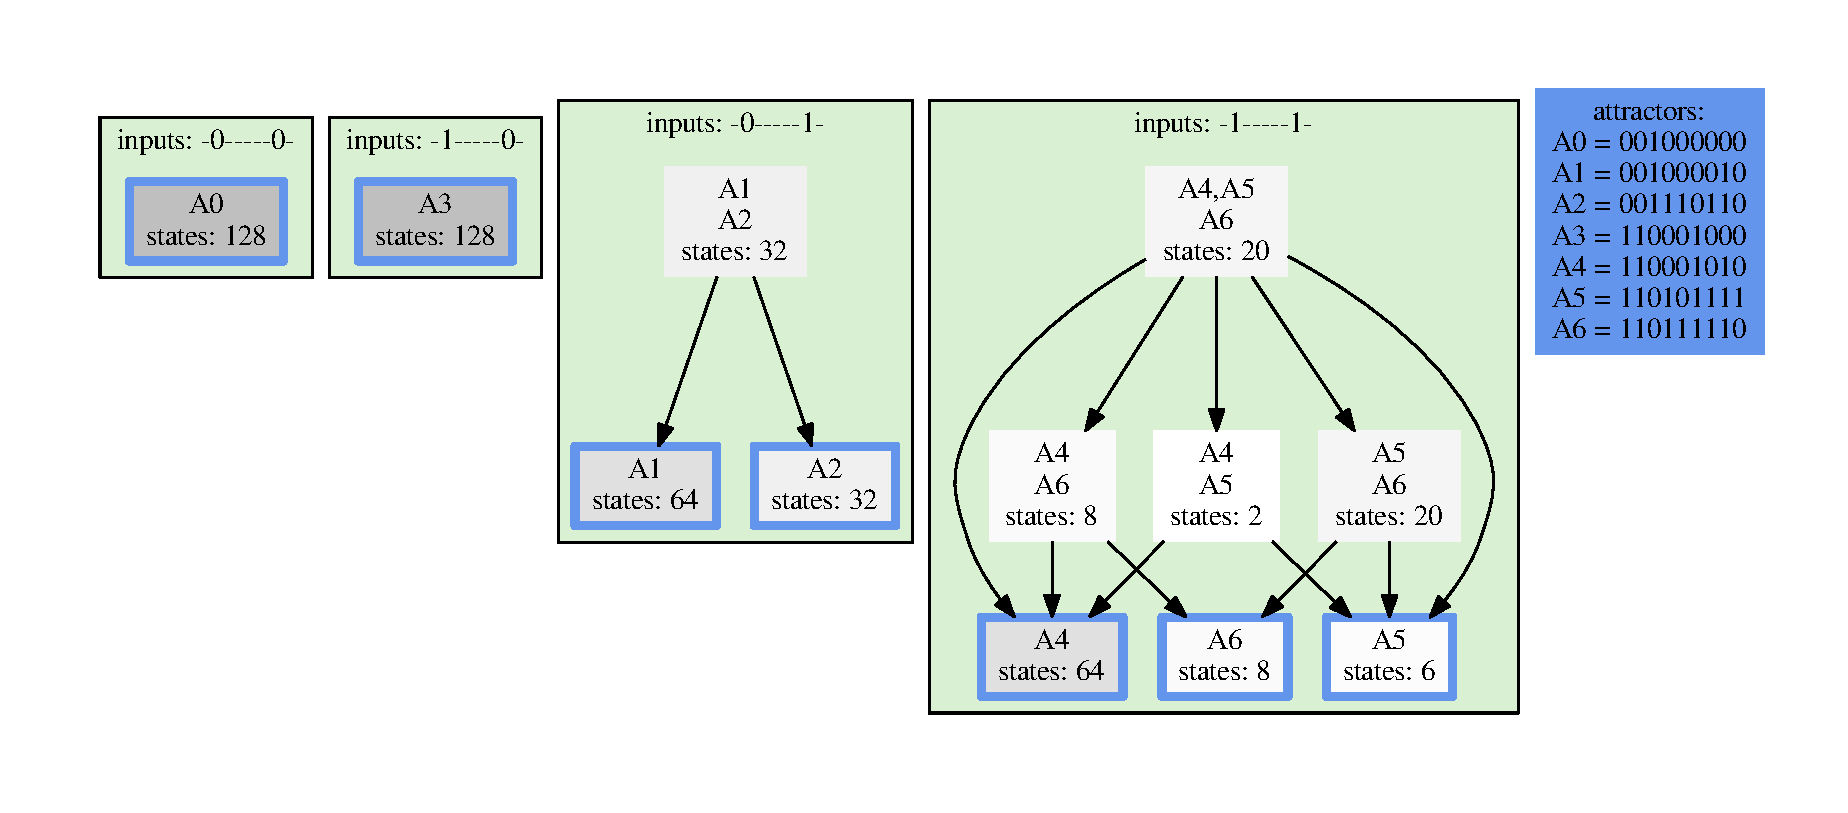
\includegraphics{figure26.pdf}}
\caption{The basin diagram of the network \emph{arellano\_rootstem} from the repository.}\label{Manual:figure26}\end{figure}

If you want to create a separate image for the basin and the states representing the attractors use the parameter \emph{FnameATTRACTORS} of the
function {\hyperref[AttractorBasins:diagram2image]{\emph{diagram2image}}}:

\begin{Verbatim}[commandchars=\\\{\}]
\PYG{g+gp}{\PYGZgt{}\PYGZgt{}\PYGZgt{} }\PYG{n}{AB}\PYG{o}{.}\PYG{n}{diagram2image}\PYG{p}{(}\PYG{n}{primes}\PYG{p}{,} \PYG{n}{diagram}\PYG{p}{,} \PYG{l+s}{\PYGZdq{}}\PYG{l+s}{diagram.pdf}\PYG{l+s}{\PYGZdq{}}\PYG{p}{,} \PYG{l+s}{\PYGZdq{}}\PYG{l+s}{attractors.pdf}\PYG{l+s}{\PYGZdq{}}\PYG{p}{)}
\end{Verbatim}

Finally, in particular for diagrams with many nodes you may want to generate the so-called aggregate diagram in which nodes
with the same number of reachable attractors are combined.
That is, all nodes that can reach, for example, exactly two attractors (irrespective of which two attractors) are represented by a single node.
An example is given in {\hyperref[Manual:figure27]{\emph{the figure below}}}:

\begin{Verbatim}[commandchars=\\\{\}]
\PYG{g+gp}{\PYGZgt{}\PYGZgt{}\PYGZgt{} }\PYG{n}{AB}\PYG{o}{.}\PYG{n}{diagram2aggregate\PYGZus{}image}\PYG{p}{(}\PYG{n}{diagram}\PYG{p}{,} \PYG{l+s}{\PYGZdq{}}\PYG{l+s}{aggregate.pdf}\PYG{l+s}{\PYGZdq{}}\PYG{p}{)}
\end{Verbatim}
\begin{figure}[htbp]
\centering
\capstart

\scalebox{1.000000}{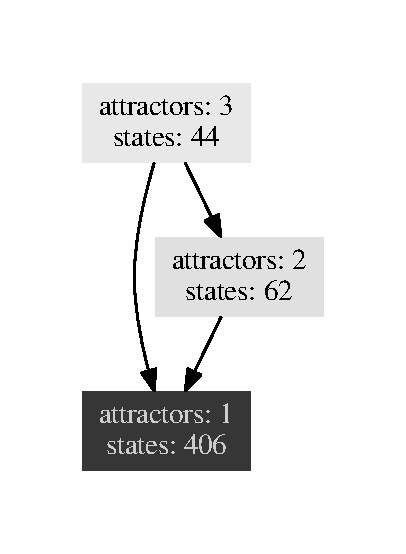
\includegraphics{figure27.pdf}}
\caption{The aggregated basin diagram of the network \emph{arellano\_rootstem} from the repository.}\label{Manual:figure27}\end{figure}


\subsection{attractor approximations}
\label{Manual:attractor-approximations}
Minimal trap spaces approximate attractors because every trap space contains an attractor.
But, there can be attractors outside of minimal trap spaces.
And there may be several attractors inside a single minmal trap space.
And an attractor inside a minimal trap space may be much smaller than the minimal trap space that contains it.
Hence there are three criteria for the quality of minimal trap spaces as approximations for attractors:
\begin{enumerate}
\item {} 
\textbf{completeness}: whether every attractor is contained in one of the network's minimal trap spaces

\item {} 
\textbf{univocality}: whether each minimal trap spaces contains exactly one attractor

\item {} 
\textbf{faithfulness}: whether the number of free variables of the minimal trap space is equal to the number of oscillating variables of the attractors contained in it

\end{enumerate}

If the minimal trap spaces of a network are complete, univocal and faithful then we say that the approximation is perfect.
So far, the minimal trap spaces of every published network we are aware of are a perfect approximation of its attractors.
Hence, although computing the attractors of asynchronous STGs is in general a hard problem,
in practice we may get away with computing their minimal trap spaces which can efficiently be done for networks with hundreds of components.
Note that for limit cycles of synchronous STGs and steady states other algorithms, e.g. {\hyperref[Bibliography:dubrova2011]{\emph{Dubrova2011}}} and \emph{Naldi2007} are more suitable.

In {\hyperref[Bibliography:klarner2015trap]{\emph{Klarner2015(a)}}} we demonstrate that completeness, univocality and faithfulness can all be decided using CTL model checking.
The functions {\hyperref[AttractorDetection:completeness]{\emph{completeness}}}, \emph{univocal} and \emph{faithful} automatically generate and test the respective queries,
which are defined in Sections 4.1, 4.2 and 4.3 of {\hyperref[Bibliography:klarner2015trap]{\emph{Klarner2015(a)}}}.

As an example of a network whose minimal trap spaces are complete, univocal and faithful
consider again the network defined in {\hyperref[Manual:figure25]{\emph{the figure above}}}.
The functions \emph{univocal} and \emph{faithful} each require the primes, update strategy and a trap space:

\begin{Verbatim}[commandchars=\\\{\}]
\PYG{g+gp}{\PYGZgt{}\PYGZgt{}\PYGZgt{} }\PYG{n}{update} \PYG{o}{=} \PYG{l+s}{\PYGZdq{}}\PYG{l+s}{asynchronous}\PYG{l+s}{\PYGZdq{}}
\PYG{g+gp}{\PYGZgt{}\PYGZgt{}\PYGZgt{} }\PYG{n}{mintspaces} \PYG{o}{=} \PYG{n}{TS}\PYG{o}{.}\PYG{n}{trap\PYGZus{}spaces}\PYG{p}{(}\PYG{n}{primes}\PYG{p}{,} \PYG{l+s}{\PYGZdq{}}\PYG{l+s}{min}\PYG{l+s}{\PYGZdq{}}\PYG{p}{)}
\PYG{g+gp}{\PYGZgt{}\PYGZgt{}\PYGZgt{} }\PYG{k}{for} \PYG{n}{x} \PYG{o+ow}{in} \PYG{n}{mintspaces}\PYG{p}{:}
\PYG{g+gp}{... }    \PYG{n}{answer\PYGZus{}univocal} \PYG{o}{=} \PYG{n}{AD}\PYG{o}{.}\PYG{n}{univocal}\PYG{p}{(}\PYG{n}{primes}\PYG{p}{,} \PYG{n}{update}\PYG{p}{,} \PYG{n}{x}\PYG{p}{)}
\PYG{g+gp}{... }    \PYG{n}{answer\PYGZus{}faithful} \PYG{o}{=} \PYG{n}{AD}\PYG{o}{.}\PYG{n}{faithful}\PYG{p}{(}\PYG{n}{primes}\PYG{p}{,} \PYG{n}{update}\PYG{p}{,} \PYG{n}{x}\PYG{p}{)}
\PYG{g+gp}{... }    \PYG{k}{print} \PYG{l+s}{\PYGZdq{}}\PYG{l+s}{min trap space:}\PYG{l+s}{\PYGZdq{}}\PYG{p}{,} \PYG{n}{STGs}\PYG{o}{.}\PYG{n}{subspace2str}\PYG{p}{(}\PYG{n}{primes}\PYG{p}{,} \PYG{n}{x}\PYG{p}{)}
\PYG{g+gp}{... }    \PYG{k}{print} \PYG{l+s}{\PYGZdq{}}\PYG{l+s}{  is univocal:}\PYG{l+s}{\PYGZdq{}}\PYG{p}{,} \PYG{n}{answer\PYGZus{}univocal}
\PYG{g+gp}{... }    \PYG{k}{print} \PYG{l+s}{\PYGZdq{}}\PYG{l+s}{  is faithful:}\PYG{l+s}{\PYGZdq{}}\PYG{p}{,} \PYG{n}{answer\PYGZus{}faithful}
\PYG{g+go}{min trap space: \PYGZhy{}10}
\PYG{g+go}{  is univocal: True}
\PYG{g+go}{  is faithful: True}
\PYG{g+go}{min trap space: 101}
\PYG{g+go}{  is univocal: True}
\PYG{g+go}{  is faithful: True}
\end{Verbatim}

The function for deciding whether the minimal trap spaces are complete requires only two arguments, the primes and the update strategy,
because it is implied that the trap spaces must be all minimal ones.
See {\hyperref[AttractorDetection:completeness]{\emph{completeness}}} for details.

\begin{Verbatim}[commandchars=\\\{\}]
\PYG{g+gp}{\PYGZgt{}\PYGZgt{}\PYGZgt{} }\PYG{n}{AD}\PYG{o}{.}\PYG{n}{completeness}\PYG{p}{(}\PYG{n}{primes}\PYG{p}{,} \PYG{n}{update}\PYG{p}{)}
\PYG{g+go}{True}
\end{Verbatim}

Since {\hyperref[AttractorDetection:univocality]{\emph{univocality}}} is based on detecting at least one attractor, via the random walk algorithm explained above,
and since a counterexample to the univocality query contains information about additional attractors,
there is a second function, called \emph{univocality\_with\_counterexample{}`returns a triplet consisting of the answer, an attractor state and a counterexample (if the trap space is not univocal),
see :ref:{}`univocality} for details.
The function {\hyperref[AttractorDetection:faithfulness-with-counterexample]{\emph{faithfulness\_with\_counterexample}}} returns a tuple that consists of the answer and a counterexample if it exists.

As an illustration, consider network (A) given in Figure 1 of {\hyperref[Bibliography:klarner2015trap]{\emph{Klarner2015(a)}}}.
It is defined by the following functions:

The resulting STG is shown in {\hyperref[Manual:figure25]{\emph{the figure below}}}.

Its STG contains two cyclic attractors and its minimal trap space \code{-{-}-} contains two cyclic attractors and it therefore not univocal.

\begin{Verbatim}[commandchars=\\\{\}]
\PYG{g+gp}{\PYGZgt{}\PYGZgt{}\PYGZgt{} }\PYG{n}{bnet} \PYG{o}{=} \PYG{p}{[}\PYG{l+s}{\PYGZdq{}}\PYG{l+s}{v1, !v1\PYGZam{}!v2\PYGZam{}v3 \textbar{} !v1\PYGZam{}v2\PYGZam{}!v3 \textbar{} v1\PYGZam{}!v2\PYGZam{}!v3 \textbar{} v1\PYGZam{}v2\PYGZam{}v3}\PYG{l+s}{\PYGZdq{}}\PYG{p}{,}
\PYG{g+gp}{... }        \PYG{l+s}{\PYGZdq{}}\PYG{l+s}{v2, !v1\PYGZam{}!v2\PYGZam{}!v3 \textbar{} !v1\PYGZam{}v2\PYGZam{}v3 \textbar{} v1\PYGZam{}!v2\PYGZam{}v3 \textbar{} v1\PYGZam{}v2\PYGZam{}!v3}\PYG{l+s}{\PYGZdq{}}\PYG{p}{,}
\PYG{g+gp}{... }        \PYG{l+s}{\PYGZdq{}}\PYG{l+s}{v3, !v1\PYGZam{}!v2\PYGZam{}v3 \textbar{} !v1\PYGZam{}v2\PYGZam{}!v3 \textbar{} v1\PYGZam{}!v2\PYGZam{}!v3 \textbar{} v1\PYGZam{}v2\PYGZam{}v3}\PYG{l+s}{\PYGZdq{}}\PYG{p}{]}
\PYG{g+gp}{\PYGZgt{}\PYGZgt{}\PYGZgt{} }\PYG{n}{bnet} \PYG{o}{=} \PYG{l+s}{\PYGZdq{}}\PYG{l+s+se}{\PYGZbs{}n}\PYG{l+s}{\PYGZdq{}}\PYG{o}{.}\PYG{n}{join}\PYG{p}{(}\PYG{n}{bnet}\PYG{p}{)}
\PYG{g+gp}{\PYGZgt{}\PYGZgt{}\PYGZgt{} }\PYG{n}{primes} \PYG{o}{=} \PYG{n}{FEX}\PYG{o}{.}\PYG{n}{bnet2primes}\PYG{p}{(}\PYG{n}{bnet}\PYG{p}{)}
\PYG{g+gp}{\PYGZgt{}\PYGZgt{}\PYGZgt{} }\PYG{n}{mintspaces} \PYG{o}{=} \PYG{n}{TS}\PYG{o}{.}\PYG{n}{trap\PYGZus{}spaces}\PYG{p}{(}\PYG{n}{primes}\PYG{p}{,} \PYG{l+s}{\PYGZdq{}}\PYG{l+s}{min}\PYG{l+s}{\PYGZdq{}}\PYG{p}{)}
\PYG{g+gp}{\PYGZgt{}\PYGZgt{}\PYGZgt{} }\PYG{n}{stg} \PYG{o}{=} \PYG{n}{STGs}\PYG{o}{.}\PYG{n}{primes2stg}\PYG{p}{(}\PYG{n}{primes}\PYG{p}{,} \PYG{l+s}{\PYGZdq{}}\PYG{l+s}{asynchronous}\PYG{l+s}{\PYGZdq{}}\PYG{p}{)}
\PYG{g+gp}{\PYGZgt{}\PYGZgt{}\PYGZgt{} }\PYG{n}{mintspaces} \PYG{o}{=} \PYG{n}{TS}\PYG{o}{.}\PYG{n}{trap\PYGZus{}spaces}\PYG{p}{(}\PYG{n}{primes}\PYG{p}{,} \PYG{l+s}{\PYGZdq{}}\PYG{l+s}{min}\PYG{l+s}{\PYGZdq{}}\PYG{p}{)}
\PYG{g+gp}{\PYGZgt{}\PYGZgt{}\PYGZgt{} }\PYG{k}{print} \PYG{p}{[}\PYG{n}{STGs}\PYG{o}{.}\PYG{n}{subspace2str}\PYG{p}{(}\PYG{n}{primes}\PYG{p}{,} \PYG{n}{x}\PYG{p}{)} \PYG{k}{for} \PYG{n}{x} \PYG{o+ow}{in} \PYG{n}{mintspaces}\PYG{p}{]}
\end{Verbatim}

\begin{Verbatim}[commandchars=\\\{\}]
\PYG{g+gp}{\PYGZgt{}\PYGZgt{}\PYGZgt{} }\PYG{n}{STGs}\PYG{o}{.}\PYG{n}{add\PYGZus{}style\PYGZus{}sccs}\PYG{p}{(}\PYG{n}{stg}\PYG{p}{)}
\PYG{g+gp}{\PYGZgt{}\PYGZgt{}\PYGZgt{} }\PYG{n}{STGs}\PYG{o}{.}\PYG{n}{add\PYGZus{}style\PYGZus{}subspaces}\PYG{p}{(}\PYG{n}{primes}\PYG{p}{,} \PYG{n}{stg}\PYG{p}{,} \PYG{n}{mintspaces}\PYG{p}{)}
\end{Verbatim}
\begin{figure}[htbp]
\centering
\capstart

\scalebox{0.600000}{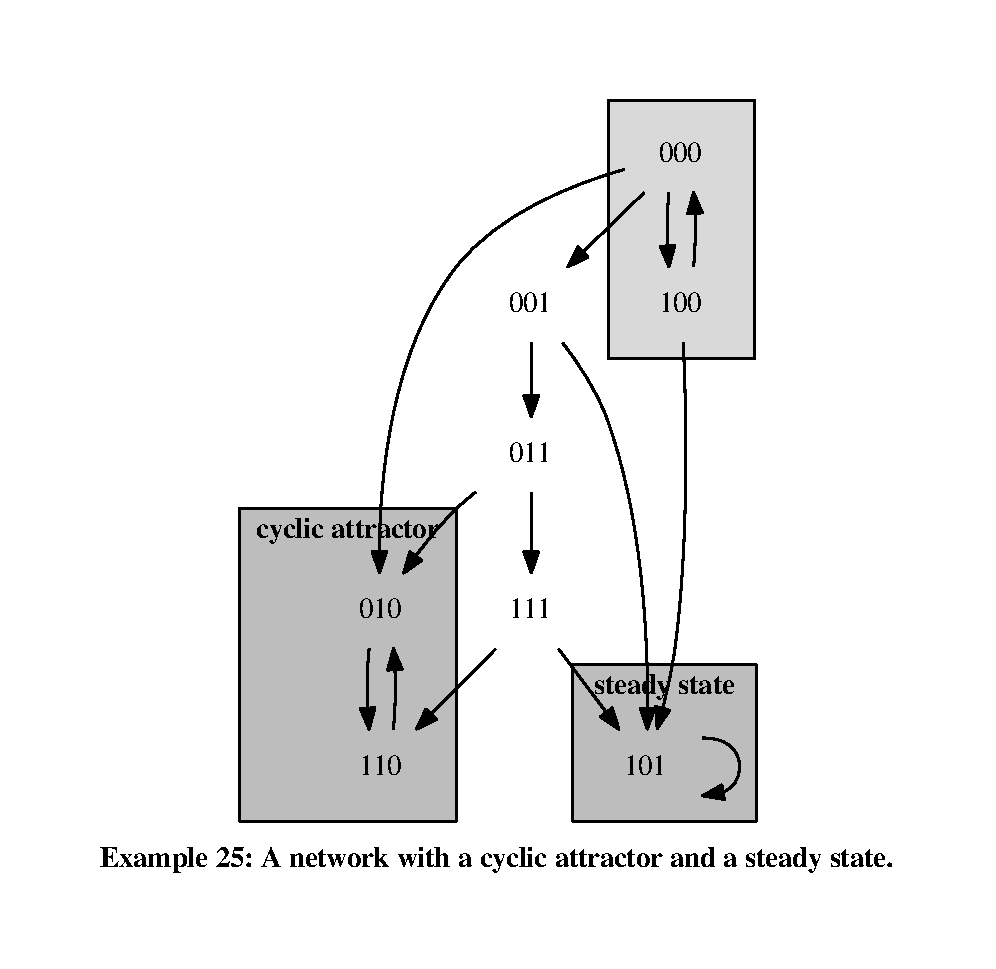
\includegraphics{figure25.pdf}}
\caption{The state transition graph \emph{``example25\_stg.pdf''} in which the minimal trap space ``---'' is not univocal.}{\small 
\begin{Verbatim}[commandchars=\\\{\}]
\PYG{g+gp}{\PYGZgt{}\PYGZgt{}\PYGZgt{} }\PYG{n}{mintspaces} \PYG{o}{=} \PYG{n}{TS}\PYG{o}{.}\PYG{n}{trap\PYGZus{}spaces}\PYG{p}{(}\PYG{n}{primes}\PYG{p}{,} \PYG{l+s}{\PYGZdq{}}\PYG{l+s}{min}\PYG{l+s}{\PYGZdq{}}\PYG{p}{)}
\PYG{g+gp}{\PYGZgt{}\PYGZgt{}\PYGZgt{} }\PYG{k}{print} \PYG{p}{[}\PYG{n}{STGs}\PYG{o}{.}\PYG{n}{subspace2str}\PYG{p}{(}\PYG{n}{primes}\PYG{p}{,} \PYG{n}{x}\PYG{p}{)} \PYG{k}{for} \PYG{n}{x} \PYG{o+ow}{in} \PYG{n}{mintspaces}\PYG{p}{]}
\PYG{g+go}{[\PYGZsq{}\PYGZhy{}\PYGZhy{}\PYGZhy{}\PYGZsq{}]}
\PYG{g+gp}{\PYGZgt{}\PYGZgt{}\PYGZgt{} }\PYG{n}{STGs}\PYG{o}{.}\PYG{n}{add\PYGZus{}style\PYGZus{}subspaces}\PYG{p}{(}\PYG{n}{stg}\PYG{p}{,} \PYG{n}{mintspaces}\PYG{p}{)}
\PYG{g+gp}{\PYGZgt{}\PYGZgt{}\PYGZgt{} }\PYG{n}{stg}\PYG{o}{.}\PYG{n}{graph}\PYG{p}{[}\PYG{l+s}{\PYGZdq{}}\PYG{l+s}{label}\PYG{l+s}{\PYGZdq{}}\PYG{p}{]} \PYG{o}{=} \PYG{l+s}{\PYGZdq{}}\PYG{l+s}{Example 26: An STG whose minimal trap space }\PYG{l+s}{\PYGZsq{}}\PYG{l+s}{\PYGZhy{}\PYGZhy{}\PYGZhy{}}\PYG{l+s}{\PYGZsq{}}\PYG{l+s}{ is not univocal}\PYG{l+s}{\PYGZdq{}}
\end{Verbatim}
}\label{Manual:id6}\end{figure}


\chapter{Reference}
\label{Reference:networkx-has-path}\label{Reference::doc}\label{Reference:reference}

\section{FileExchange}
\label{FileExchange:fileexchange}\label{FileExchange::doc}\label{FileExchange:id1}

\subsection{bnet2primes}
\label{FileExchange:id2}\label{FileExchange:bnet2primes}\index{bnet2primes() (in module PyBoolNet.FileExchange)}

\begin{fulllineitems}
\phantomsection\label{FileExchange:PyBoolNet.FileExchange.bnet2primes}\pysiglinewithargsret{\bfcode{bnet2primes}}{\emph{BNET}, \emph{FnamePRIMES=None}}{}
Generates and returns the prime implicants of a Boolean network in {\hyperref[Installation:installation-boolnet]{\emph{BoolNet}}} format.
The primes are saved as a \emph{json} file if \emph{FnamePRIMES} is given.
The argument \emph{BNET} may be either the name of a \emph{bnet} file or a string containing the file contents.
Use the function {\hyperref[FileExchange:read-primes]{\emph{FileExchange.read\_primes}}} to open a previously saved \emph{json} file.

\begin{notice}{note}{Note:}
Requires the program {\hyperref[Installation:installation-bnettoprime]{\emph{BNetToPrime}}}.
\end{notice}
\begin{description}
\item[{\textbf{arguments}:}] \leavevmode\begin{itemize}
\item {} 
\emph{BNET}: name of \emph{bnet} file or string contents of file

\item {} 
\emph{FnamePRIMES}: \emph{None} or name of \emph{json} file to save primes

\end{itemize}

\item[{\textbf{returns}:    }] \leavevmode\begin{itemize}
\item {} 
\emph{Primes}: prime implicants

\end{itemize}

\end{description}

\textbf{example}:

\begin{Verbatim}[commandchars=\\\{\}]
\PYG{g+gp}{\PYGZgt{}\PYGZgt{}\PYGZgt{} }\PYG{n}{primes} \PYG{o}{=} \PYG{n}{bnet2primes}\PYG{p}{(}\PYG{l+s}{\PYGZdq{}}\PYG{l+s}{mapk.bnet}\PYG{l+s}{\PYGZdq{}}\PYG{p}{,} \PYG{l+s}{\PYGZdq{}}\PYG{l+s}{mapk.primes}\PYG{l+s}{\PYGZdq{}} \PYG{p}{)}
\PYG{g+gp}{\PYGZgt{}\PYGZgt{}\PYGZgt{} }\PYG{n}{primes} \PYG{o}{=} \PYG{n}{bnet2primes}\PYG{p}{(}\PYG{l+s}{\PYGZdq{}}\PYG{l+s}{mapk.bnet}\PYG{l+s}{\PYGZdq{}}\PYG{p}{)}
\PYG{g+gp}{\PYGZgt{}\PYGZgt{}\PYGZgt{} }\PYG{n}{primes} \PYG{o}{=} \PYG{n}{bnet2primes}\PYG{p}{(}\PYG{l+s}{\PYGZdq{}}\PYG{l+s}{Erk, !Mek }\PYG{l+s+se}{\PYGZbs{}n}\PYG{l+s}{ Raf, Ras \PYGZam{} Mek}\PYG{l+s}{\PYGZdq{}}\PYG{p}{)}
\PYG{g+gp}{\PYGZgt{}\PYGZgt{}\PYGZgt{} }\PYG{n}{primes} \PYG{o}{=} \PYG{n}{bnet2primes}\PYG{p}{(}\PYG{l+s}{\PYGZdq{}}\PYG{l+s}{Erk, !Mek }\PYG{l+s+se}{\PYGZbs{}n}\PYG{l+s}{ Raf, Ras \PYGZam{} Mek}\PYG{l+s}{\PYGZdq{}}\PYG{p}{,} \PYG{l+s}{\PYGZdq{}}\PYG{l+s}{mapk.primes}\PYG{l+s}{\PYGZdq{}}\PYG{p}{)}
\end{Verbatim}

\end{fulllineitems}



\subsection{primes2bnet}
\label{FileExchange:primes2bnet}\label{FileExchange:id3}\index{primes2bnet() (in module PyBoolNet.FileExchange)}

\begin{fulllineitems}
\phantomsection\label{FileExchange:PyBoolNet.FileExchange.primes2bnet}\pysiglinewithargsret{\bfcode{primes2bnet}}{\emph{Primes}, \emph{FnameBNET=None}, \emph{Minimize=False}, \emph{Header=False}}{}
Saves \emph{Primes} as a \emph{bnet} file, including the header \emph{``targets, factors''} for compatibility with {\hyperref[Installation:installation-boolnet]{\emph{BoolNet}}}.
Without minimization, the resuting formulas are disjunctions of all prime implicants and may therefore be very long.
If \emph{Minimize=True} then a Python version of the Quine-McCluskey algorithm,
namely {\hyperref[Bibliography:prekas2012]{\emph{Prekas2012}}} which is implemented in {\hyperref[QuineMcCluskey:primes2mindnf]{\emph{QuineMcCluskey.primes2mindnf}}},
will be used to minimize the number of clauses for each update function.
\begin{description}
\item[{\textbf{arguments}:}] \leavevmode\begin{itemize}
\item {} 
\emph{Primes}: prime implicants

\item {} 
\emph{FnameBNET} (str): name of \emph{bnet} file or \emph{None} for the string of the file contents

\item {} 
\emph{Minimize} (bool): whether the expressions should be minimized

\item {} 
\emph{Header} (bool): whether to include the ``targets, factors'' header

\end{itemize}

\item[{\textbf{returns}:}] \leavevmode\begin{itemize}
\item {} 
\emph{BNET} (str) if \emph{FnameBNET=None} or \emph{None} otherwise

\end{itemize}

\end{description}

\textbf{example}:

\begin{Verbatim}[commandchars=\\\{\}]
\PYG{g+gp}{\PYGZgt{}\PYGZgt{}\PYGZgt{} }\PYG{n}{primes2bnet}\PYG{p}{(}\PYG{n}{primes}\PYG{p}{,} \PYG{l+s}{\PYGZdq{}}\PYG{l+s}{mapk.bnet}\PYG{l+s}{\PYGZdq{}}\PYG{p}{)}
\PYG{g+gp}{\PYGZgt{}\PYGZgt{}\PYGZgt{} }\PYG{n}{primes2bnet}\PYG{p}{(}\PYG{n}{primes}\PYG{p}{,} \PYG{l+s}{\PYGZdq{}}\PYG{l+s}{mapk.bnet}\PYG{l+s}{\PYGZdq{}}\PYG{p}{,} \PYG{n+nb+bp}{True}\PYG{p}{)}
\PYG{g+gp}{\PYGZgt{}\PYGZgt{}\PYGZgt{} }\PYG{n}{expr} \PYG{o}{=} \PYG{n}{primes2bnet}\PYG{p}{(}\PYG{n}{primes}\PYG{p}{)}
\PYG{g+gp}{\PYGZgt{}\PYGZgt{}\PYGZgt{} }\PYG{n}{expr} \PYG{o}{=} \PYG{n}{primes2bnet}\PYG{p}{(}\PYG{n}{primes}\PYG{p}{,} \PYG{n+nb+bp}{True}\PYG{p}{)}
\end{Verbatim}

\end{fulllineitems}



\subsection{write\_primes}
\label{FileExchange:write-primes}\label{FileExchange:id4}\index{write\_primes() (in module PyBoolNet.FileExchange)}

\begin{fulllineitems}
\phantomsection\label{FileExchange:PyBoolNet.FileExchange.write_primes}\pysiglinewithargsret{\bfcode{write\_primes}}{\emph{Primes}, \emph{FnamePRIMES}}{}
Saves \emph{Primes} as a \emph{json} file.
\begin{description}
\item[{\textbf{arguments}:}] \leavevmode\begin{itemize}
\item {} 
\emph{Primes}: prime implicants

\item {} 
\emph{FnamePRIMES} (str): name of \emph{json} file

\end{itemize}

\end{description}

\textbf{example}:

\begin{Verbatim}[commandchars=\\\{\}]
\PYG{g+gp}{\PYGZgt{}\PYGZgt{}\PYGZgt{} }\PYG{n}{write\PYGZus{}primes}\PYG{p}{(}\PYG{n}{primes}\PYG{p}{,} \PYG{l+s}{\PYGZdq{}}\PYG{l+s}{mapk.primes}\PYG{l+s}{\PYGZdq{}}\PYG{p}{)}
\end{Verbatim}

\end{fulllineitems}



\subsection{read\_primes}
\label{FileExchange:id5}\label{FileExchange:read-primes}\index{read\_primes() (in module PyBoolNet.FileExchange)}

\begin{fulllineitems}
\phantomsection\label{FileExchange:PyBoolNet.FileExchange.read_primes}\pysiglinewithargsret{\bfcode{read\_primes}}{\emph{FnamePRIMES}}{}
Reads the prime implicants of a Boolean network that were previously stored as a \emph{json} file.
\begin{description}
\item[{\textbf{arguments}:}] \leavevmode\begin{itemize}
\item {} 
\emph{FnamePRIMES} (str): name of \emph{json} file

\end{itemize}

\item[{\textbf{returns}:}] \leavevmode\begin{itemize}
\item {} 
\emph{Primes}: prime implicants

\end{itemize}

\end{description}

\textbf{example}:

\begin{Verbatim}[commandchars=\\\{\}]
\PYG{g+gp}{\PYGZgt{}\PYGZgt{}\PYGZgt{} }\PYG{n}{primes} \PYG{o}{=} \PYG{n}{read\PYGZus{}primes}\PYG{p}{(}\PYG{l+s}{\PYGZdq{}}\PYG{l+s}{mapk.primes}\PYG{l+s}{\PYGZdq{}}\PYG{p}{)}
\end{Verbatim}

\end{fulllineitems}



\subsection{primes2genysis}
\label{FileExchange:id6}\label{FileExchange:primes2genysis}\index{primes2genysis() (in module PyBoolNet.FileExchange)}

\begin{fulllineitems}
\phantomsection\label{FileExchange:PyBoolNet.FileExchange.primes2genysis}\pysiglinewithargsret{\bfcode{primes2genysis}}{\emph{Primes}, \emph{FnameGENYSIS}}{}
Generates a \href{http://www.vital-it.ch/software/genYsis}{GenYsis} file from \emph{Primes} for the computation of all attractors of the synchronous or asynchronous transition system.
\href{http://www.vital-it.ch/software/genYsis}{GenYsis} was introduced in {\hyperref[Bibliography:garg2008]{\emph{Garg2008}}}.
It is available at \href{http://www.vital-it.ch/software/genYsis}{http://www.vital-it.ch/software/genYsis}.
\begin{description}
\item[{\textbf{arguments}:}] \leavevmode\begin{itemize}
\item {} 
\emph{Primes}: prime implicants

\item {} 
\emph{FnameGENYSIS} (str): name of \href{http://www.vital-it.ch/software/genYsis}{GenYsis} file

\end{itemize}

\end{description}

\textbf{example}:

\begin{Verbatim}[commandchars=\\\{\}]
\PYG{g+gp}{\PYGZgt{}\PYGZgt{}\PYGZgt{} }\PYG{n}{primes2genysis}\PYG{p}{(}\PYG{n}{primes}\PYG{p}{,} \PYG{l+s}{\PYGZdq{}}\PYG{l+s}{mapk.genysis}\PYG{l+s}{\PYGZdq{}}\PYG{p}{)}
\end{Verbatim}

\end{fulllineitems}



\subsection{primes2bns}
\label{FileExchange:id7}\label{FileExchange:primes2bns}\index{primes2bns() (in module PyBoolNet.FileExchange)}

\begin{fulllineitems}
\phantomsection\label{FileExchange:PyBoolNet.FileExchange.primes2bns}\pysiglinewithargsret{\bfcode{primes2bns}}{\emph{Primes}, \emph{FnameBNS}}{}
Saves Primes as a \emph{bns} file for the computation of all attractors of the synchronous transition system.
\href{https://people.kth.se/~dubrova/bns.html}{BNS} is based on {\hyperref[Bibliography:dubrova2011]{\emph{Dubrova2011}}}.
It is available at \href{http://people.kth.se/~dubrova/bns.html}{http://people.kth.se/\textasciitilde{}dubrova/bns.html}.
\begin{description}
\item[{\textbf{arguments}:}] \leavevmode\begin{itemize}
\item {} 
\emph{Primes}: prime implicants

\item {} 
\emph{FnameBNS} (str): name of \emph{bns} file

\end{itemize}

\end{description}

\textbf{example}:

\begin{Verbatim}[commandchars=\\\{\}]
\PYG{g+gp}{\PYGZgt{}\PYGZgt{}\PYGZgt{} }\PYG{n}{primes2bns}\PYG{p}{(}\PYG{n}{primes}\PYG{p}{,} \PYG{l+s}{\PYGZdq{}}\PYG{l+s}{mapk.bns}\PYG{l+s}{\PYGZdq{}}\PYG{p}{)}
\end{Verbatim}

\end{fulllineitems}



\subsection{primes2eqn}
\label{FileExchange:primes2eqn}\label{FileExchange:id8}\index{primes2eqn() (in module PyBoolNet.FileExchange)}

\begin{fulllineitems}
\phantomsection\label{FileExchange:PyBoolNet.FileExchange.primes2eqn}\pysiglinewithargsret{\bfcode{primes2eqn}}{\emph{Primes}, \emph{FnameEQN}}{}
Generates a \emph{eqn} file as specified in the manual for the model checking software \href{http://turing.iimas.unam.mx:8080/AntelopeWEB/content/about.jsp}{Antelope} from \emph{Primes}.
\href{http://turing.iimas.unam.mx:8080/AntelopeWEB/content/about.jsp}{Antelope} was introduced in {\hyperref[Bibliography:arellano2011]{\emph{Arellano2011}}}.
\begin{description}
\item[{\textbf{arguments}:}] \leavevmode\begin{itemize}
\item {} 
\emph{Primes}: prime implicants

\item {} 
\emph{FnameEQN} (str): name of \emph{eqn} file

\end{itemize}

\end{description}

\textbf{example}:

\begin{Verbatim}[commandchars=\\\{\}]
\PYG{g+gp}{\PYGZgt{}\PYGZgt{}\PYGZgt{} }\PYG{n}{primes2eqn}\PYG{p}{(}\PYG{n}{primes}\PYG{p}{,} \PYG{l+s}{\PYGZdq{}}\PYG{l+s}{mapk.eqn}\PYG{l+s}{\PYGZdq{}}\PYG{p}{)}
\end{Verbatim}

\end{fulllineitems}



\section{PrimeImplicants}
\label{PrimeImplicants:networkx-has-path}\label{PrimeImplicants::doc}\label{PrimeImplicants:primeimplicants}\label{PrimeImplicants:id1}

\subsection{copy}
\label{PrimeImplicants:copy}\label{PrimeImplicants:primes-copy}\index{copy() (in module PyBoolNet.PrimeImplicants)}

\begin{fulllineitems}
\phantomsection\label{PrimeImplicants:PyBoolNet.PrimeImplicants.copy}\pysiglinewithargsret{\bfcode{copy}}{\emph{Primes}}{}
Creates a copy of \emph{Primes}.
\begin{description}
\item[{\textbf{arguments}:}] \leavevmode\begin{itemize}
\item {} 
\emph{Primes}: prime implicants

\end{itemize}

\item[{\textbf{returns}:}] \leavevmode\begin{itemize}
\item {} 
\emph{PrimesNew} (dict): a copy of \emph{Primes}

\end{itemize}

\end{description}

\textbf{example}:

\begin{Verbatim}[commandchars=\\\{\}]
\PYG{g+gp}{\PYGZgt{}\PYGZgt{}\PYGZgt{} }\PYG{n}{primes\PYGZus{}new} \PYG{o}{=} \PYG{n}{copy}\PYG{p}{(}\PYG{n}{primes}\PYG{p}{)}
\end{Verbatim}

\end{fulllineitems}



\subsection{are\_equal}
\label{PrimeImplicants:id2}\label{PrimeImplicants:are-equal}\index{are\_equal() (in module PyBoolNet.PrimeImplicants)}

\begin{fulllineitems}
\phantomsection\label{PrimeImplicants:PyBoolNet.PrimeImplicants.are_equal}\pysiglinewithargsret{\bfcode{are\_equal}}{\emph{Primes1}, \emph{Primes2}}{}
Tests whether \emph{Primes1} and \emph{Primes2} are equal.
The dictionary comparison \emph{Primes1 == Primes2} does in general not work because the clauses of each may not be in the same order.
\begin{description}
\item[{\textbf{arguments}:}] \leavevmode\begin{itemize}
\item {} 
\emph{Primes1}, \emph{Primes2}: prime implicants

\end{itemize}

\item[{\textbf{returns}:}] \leavevmode\begin{itemize}
\item {} 
\emph{Answer} (bool): whether \emph{Primes1=Primes2}

\end{itemize}

\end{description}

\textbf{example}:

\begin{Verbatim}[commandchars=\\\{\}]
\PYG{g+gp}{\PYGZgt{}\PYGZgt{}\PYGZgt{} }\PYG{n}{are\PYGZus{}equal}\PYG{p}{(}\PYG{n}{primes1}\PYG{p}{,} \PYG{n}{primes2}\PYG{p}{)}
\PYG{g+go}{True}
\end{Verbatim}

\end{fulllineitems}



\subsection{find\_inputs}
\label{PrimeImplicants:id3}\label{PrimeImplicants:find-inputs}\index{find\_inputs() (in module PyBoolNet.PrimeImplicants)}

\begin{fulllineitems}
\phantomsection\label{PrimeImplicants:PyBoolNet.PrimeImplicants.find_inputs}\pysiglinewithargsret{\bfcode{find\_inputs}}{\emph{Primes}}{}
Finds all inputs in the network defined by \emph{Primes}.
\begin{description}
\item[{\textbf{arguments}:}] \leavevmode\begin{itemize}
\item {} 
\emph{Primes}: prime implicants

\end{itemize}

\item[{\textbf{returns}:}] \leavevmode\begin{itemize}
\item {} 
\emph{Names} (list): the names of the inputs

\end{itemize}

\end{description}

\textbf{example}:

\begin{Verbatim}[commandchars=\\\{\}]
\PYG{g+gp}{\PYGZgt{}\PYGZgt{}\PYGZgt{} }\PYG{n}{find\PYGZus{}inputs}\PYG{p}{(}\PYG{n}{primes}\PYG{p}{)}
\PYG{g+go}{[\PYGZsq{}DNA\PYGZus{}damage\PYGZsq{},\PYGZsq{}EGFR\PYGZsq{},\PYGZsq{}FGFR3\PYGZsq{}]}
\end{Verbatim}

\end{fulllineitems}



\subsection{find\_outputs}
\label{PrimeImplicants:id4}\label{PrimeImplicants:find-outputs}\index{find\_outputs() (in module PyBoolNet.PrimeImplicants)}

\begin{fulllineitems}
\phantomsection\label{PrimeImplicants:PyBoolNet.PrimeImplicants.find_outputs}\pysiglinewithargsret{\bfcode{find\_outputs}}{\emph{Primes}}{}
Finds all outputs in the network defined by \emph{Primes}.
\begin{description}
\item[{\textbf{arguments}:}] \leavevmode\begin{itemize}
\item {} 
\emph{Primes}: prime implicants

\end{itemize}

\item[{\textbf{returns}:}] \leavevmode\begin{itemize}
\item {} 
\emph{Names} (list): the names of the outputs

\end{itemize}

\end{description}

\textbf{example}:

\begin{Verbatim}[commandchars=\\\{\}]
\PYG{g+gp}{\PYGZgt{}\PYGZgt{}\PYGZgt{} }\PYG{n}{find\PYGZus{}inputs}\PYG{p}{(}\PYG{n}{primes}\PYG{p}{)}
\PYG{g+go}{[\PYGZsq{}Proliferation\PYGZsq{},\PYGZsq{}Apoptosis\PYGZsq{},\PYGZsq{}GrowthArrest\PYGZsq{}]}
\end{Verbatim}

\end{fulllineitems}



\subsection{find\_constants}
\label{PrimeImplicants:id5}\label{PrimeImplicants:find-constants}\index{find\_constants() (in module PyBoolNet.PrimeImplicants)}

\begin{fulllineitems}
\phantomsection\label{PrimeImplicants:PyBoolNet.PrimeImplicants.find_constants}\pysiglinewithargsret{\bfcode{find\_constants}}{\emph{Primes}}{}
Finds all constants in the network defined by \emph{Primes}.
\begin{description}
\item[{\textbf{arguments}:}] \leavevmode\begin{itemize}
\item {} 
\emph{Primes}: prime implicants

\end{itemize}

\item[{\textbf{returns}:}] \leavevmode\begin{itemize}
\item {} 
\emph{Activities} (dict): the names and activities of constants

\end{itemize}

\end{description}

\textbf{example}:

\begin{Verbatim}[commandchars=\\\{\}]
\PYG{g+gp}{\PYGZgt{}\PYGZgt{}\PYGZgt{} }\PYG{n}{find\PYGZus{}constants}\PYG{p}{(}\PYG{n}{primes}\PYG{p}{)}
\PYG{g+go}{\PYGZob{}\PYGZsq{}CGC\PYGZsq{}:1,\PYGZsq{}IFNAR1\PYGZsq{}:1,\PYGZsq{}IFNAR2\PYGZsq{}:0,\PYGZsq{}IL4RA\PYGZsq{}:1\PYGZcb{}}
\end{Verbatim}

\end{fulllineitems}



\subsection{create\_constants}
\label{PrimeImplicants:id6}\label{PrimeImplicants:create-constants}\index{create\_constants() (in module PyBoolNet.PrimeImplicants)}

\begin{fulllineitems}
\phantomsection\label{PrimeImplicants:PyBoolNet.PrimeImplicants.create_constants}\pysiglinewithargsret{\bfcode{create\_constants}}{\emph{Primes}, \emph{Constants}, \emph{Copy=False}}{}
Creates a constant in \emph{Primes} for every name, value pair in \emph{Constants}.
Names that already exist in \emph{Primes} are overwritten.
\begin{description}
\item[{\textbf{arguments}:}] \leavevmode\begin{itemize}
\item {} 
\emph{Primes}: prime implicants

\item {} 
\emph{Constants} (dict): names and values

\item {} 
\emph{Copy} (bool): change \emph{Primes} in place or copy and return

\end{itemize}

\item[{\textbf{returns}:}] \leavevmode\begin{itemize}
\item {} 
\emph{NewPrimes} if \emph{Copy=True}

\item {} 
\emph{None} else

\end{itemize}

\end{description}

\textbf{example}:

\begin{Verbatim}[commandchars=\\\{\}]
\PYG{g+gp}{\PYGZgt{}\PYGZgt{}\PYGZgt{} }\PYG{n}{create\PYGZus{}constants}\PYG{p}{(}\PYG{n}{primes}\PYG{p}{,} \PYG{p}{\PYGZob{}}\PYG{l+s}{\PYGZdq{}}\PYG{l+s}{p53}\PYG{l+s}{\PYGZdq{}}\PYG{p}{:}\PYG{l+m+mi}{1}\PYG{p}{,} \PYG{l+s}{\PYGZdq{}}\PYG{l+s}{p21}\PYG{l+s}{\PYGZdq{}}\PYG{p}{:}\PYG{l+m+mi}{0}\PYG{p}{\PYGZcb{}}\PYG{p}{)}
\end{Verbatim}

\end{fulllineitems}



\subsection{create\_inputs}
\label{PrimeImplicants:id7}\label{PrimeImplicants:create-inputs}\index{create\_inputs() (in module PyBoolNet.PrimeImplicants)}

\begin{fulllineitems}
\phantomsection\label{PrimeImplicants:PyBoolNet.PrimeImplicants.create_inputs}\pysiglinewithargsret{\bfcode{create\_inputs}}{\emph{Primes}, \emph{Names}, \emph{Copy=False}}{}
Creates an input for every member of \emph{Names}.
Variables that already exist in \emph{Primes} are overwritten.

\begin{notice}{note}{Note:}
Suppose that a given network has constants, e.g.:

\begin{Verbatim}[commandchars=\\\{\}]
\PYG{g+gp}{\PYGZgt{}\PYGZgt{}\PYGZgt{} }\PYG{n+nb}{len}\PYG{p}{(}\PYG{n}{find\PYGZus{}constants}\PYG{p}{(}\PYG{n}{primes}\PYG{p}{)}\PYG{p}{)}\PYG{o}{\PYGZgt{}}\PYG{l+m+mi}{0}
\PYG{g+go}{True}
\end{Verbatim}

Too analyze how the network behaves under all possible values for these constants, turn them into inputs:

\begin{Verbatim}[commandchars=\\\{\}]
\PYG{g+gp}{\PYGZgt{}\PYGZgt{}\PYGZgt{} }\PYG{n}{constants} \PYG{o}{=} \PYG{n}{find\PYGZus{}constants}\PYG{p}{(}\PYG{n}{primes}\PYG{p}{)}
\PYG{g+gp}{\PYGZgt{}\PYGZgt{}\PYGZgt{} }\PYG{n}{create\PYGZus{}inputs}\PYG{p}{(}\PYG{n}{primes}\PYG{p}{,} \PYG{n}{constants}\PYG{p}{)}
\end{Verbatim}
\end{notice}
\begin{description}
\item[{\textbf{arguments}:}] \leavevmode\begin{itemize}
\item {} 
\emph{Primes}: prime implicants

\item {} 
\emph{Names} (list): variables to become constants

\item {} 
\emph{Copy} (bool): change \emph{Primes} in place or copy and return

\end{itemize}

\item[{\textbf{returns}:}] \leavevmode\begin{itemize}
\item {} 
\emph{NewPrimes} if \emph{Copy=True}

\item {} 
\emph{None} else

\end{itemize}

\end{description}

\textbf{example}:

\begin{Verbatim}[commandchars=\\\{\}]
\PYG{g+gp}{\PYGZgt{}\PYGZgt{}\PYGZgt{} }\PYG{n}{names} \PYG{o}{=} \PYG{p}{[}\PYG{l+s}{\PYGZdq{}}\PYG{l+s}{p21}\PYG{l+s}{\PYGZdq{}}\PYG{p}{,} \PYG{l+s}{\PYGZdq{}}\PYG{l+s}{p53}\PYG{l+s}{\PYGZdq{}}\PYG{p}{]}
\PYG{g+gp}{\PYGZgt{}\PYGZgt{}\PYGZgt{} }\PYG{n}{create\PYGZus{}inputs}\PYG{p}{(}\PYG{n}{primes}\PYG{p}{,} \PYG{n}{names}\PYG{p}{)}
\end{Verbatim}

\end{fulllineitems}



\subsection{create\_blinkers}
\label{PrimeImplicants:create-blinkers}\label{PrimeImplicants:id8}\index{create\_blinkers() (in module PyBoolNet.PrimeImplicants)}

\begin{fulllineitems}
\phantomsection\label{PrimeImplicants:PyBoolNet.PrimeImplicants.create_blinkers}\pysiglinewithargsret{\bfcode{create\_blinkers}}{\emph{Primes}, \emph{Names}, \emph{Copy=False}}{}
Creates a blinker for every member of \emph{Names}.
Variables that alrerady exist in \emph{Primes} are overwritten.
A blinker is a variable with in-degree one and negative auto-regulation.
Blinkers can therefore change their activity in every state of the transition system.

\begin{notice}{note}{Note:}
Suppose that a given network has a lot of inputs, e.g.:

\begin{Verbatim}[commandchars=\\\{\}]
\PYG{g+gp}{\PYGZgt{}\PYGZgt{}\PYGZgt{} }\PYG{n+nb}{len}\PYG{p}{(}\PYG{n}{find\PYGZus{}inputs}\PYG{p}{(}\PYG{n}{primes}\PYG{p}{)}\PYG{p}{)}
\PYG{g+go}{20}
\end{Verbatim}

Since input combinations define trap spaces, see e.g. {\hyperref[Bibliography:klarner2015approx]{\emph{Klarner2015(b)}}} Sec. 5.1,
all of which contain at least one minimal trap space,
it follows that the network has at least 2\textasciicircum{}20 minimal trap spaces - too many to enumerate.
To find out how non-input variables stabilize in minimal trap spaces turn the inputs into blinkers:

\begin{Verbatim}[commandchars=\\\{\}]
\PYG{g+gp}{\PYGZgt{}\PYGZgt{}\PYGZgt{} }\PYG{n}{inputs} \PYG{o}{=} \PYG{n}{find\PYGZus{}inputs}\PYG{p}{(}\PYG{n}{primes}\PYG{p}{)}
\PYG{g+gp}{\PYGZgt{}\PYGZgt{}\PYGZgt{} }\PYG{n}{create\PYGZus{}blinkers}\PYG{p}{(}\PYG{n}{primes}\PYG{p}{,} \PYG{n}{inputs}\PYG{p}{)}
\PYG{g+gp}{\PYGZgt{}\PYGZgt{}\PYGZgt{} }\PYG{n}{tspaces} \PYG{o}{=} \PYG{n}{TS}\PYG{o}{.}\PYG{n}{trap\PYGZus{}spaces}\PYG{p}{(}\PYG{n}{primes}\PYG{p}{,} \PYG{l+s}{\PYGZdq{}}\PYG{l+s}{min}\PYG{l+s}{\PYGZdq{}}\PYG{p}{)}
\end{Verbatim}
\end{notice}
\begin{description}
\item[{\textbf{arguments}:}] \leavevmode\begin{itemize}
\item {} 
\emph{Primes}: prime implicants

\item {} 
\emph{Names} (list): variables to become blinkers

\item {} 
\emph{Copy} (bool): change \emph{Primes} in place or copy and return

\end{itemize}

\item[{\textbf{returns}:}] \leavevmode\begin{itemize}
\item {} 
\emph{NewPrimes} if \emph{Copy=True}

\item {} 
\emph{None} else

\end{itemize}

\end{description}

\textbf{example}:

\begin{Verbatim}[commandchars=\\\{\}]
\PYG{g+gp}{\PYGZgt{}\PYGZgt{}\PYGZgt{} }\PYG{n}{names} \PYG{o}{=} \PYG{p}{[}\PYG{l+s}{\PYGZdq{}}\PYG{l+s}{p21}\PYG{l+s}{\PYGZdq{}}\PYG{p}{,} \PYG{l+s}{\PYGZdq{}}\PYG{l+s}{p53}\PYG{l+s}{\PYGZdq{}}\PYG{p}{]}
\PYG{g+gp}{\PYGZgt{}\PYGZgt{}\PYGZgt{} }\PYG{n}{create\PYGZus{}blinkers}\PYG{p}{(}\PYG{n}{primes}\PYG{p}{,} \PYG{n}{names}\PYG{p}{)}
\end{Verbatim}

\end{fulllineitems}



\subsection{create\_variables}
\label{PrimeImplicants:create-variables}\label{PrimeImplicants:id9}\index{create\_variables() (in module PyBoolNet.PrimeImplicants)}

\begin{fulllineitems}
\phantomsection\label{PrimeImplicants:PyBoolNet.PrimeImplicants.create_variables}\pysiglinewithargsret{\bfcode{create\_variables}}{\emph{Primes}, \emph{UpdateFunctions}, \emph{Copy=False}}{}
Creates the variables defined in \emph{UpdateFunctions} and add them to \emph{Primes}.
Variables that already exist in \emph{Primes} are overwritten.
Raises an exception if the resulting primes contain undefined variables.
The \emph{UpdateFunctions} are given as a dictionary of names and functions that are either a bnet string or a Python function.
\begin{description}
\item[{\textbf{arguments}:}] \leavevmode\begin{itemize}
\item {} 
\emph{Primes}: prime implicants

\item {} 
\emph{UpdateFunctions} (dict): a dictionary of names and update functions

\item {} 
\emph{Copy} (bool): change \emph{Primes} in place or copy and return

\end{itemize}

\item[{\textbf{returns}:}] \leavevmode\begin{itemize}
\item {} 
\emph{NewPrimes} if \emph{Copy=True}

\item {} 
\emph{None} else

\end{itemize}

\end{description}

\textbf{example}:

\begin{Verbatim}[commandchars=\\\{\}]
\PYG{g+gp}{\PYGZgt{}\PYGZgt{}\PYGZgt{} }\PYG{n}{primes} \PYG{o}{=} \PYG{n}{FileExchange}\PYG{o}{.}\PYG{n}{bnet2primes}\PYG{p}{(}\PYG{l+s}{\PYGZdq{}}\PYG{l+s}{A, A}\PYG{l+s}{\PYGZdq{}}\PYG{p}{)}
\PYG{g+gp}{\PYGZgt{}\PYGZgt{}\PYGZgt{} }\PYG{n}{create\PYGZus{}variables}\PYG{p}{(}\PYG{n}{primes}\PYG{p}{,} \PYG{p}{\PYGZob{}}\PYG{l+s}{\PYGZdq{}}\PYG{l+s}{B}\PYG{l+s}{\PYGZdq{}}\PYG{p}{:} \PYG{l+s}{\PYGZdq{}}\PYG{l+s}{A}\PYG{l+s}{\PYGZdq{}}\PYG{p}{\PYGZcb{}}\PYG{p}{)}
\PYG{g+gp}{\PYGZgt{}\PYGZgt{}\PYGZgt{} }\PYG{n}{create\PYGZus{}variables}\PYG{p}{(}\PYG{n}{primes}\PYG{p}{,} \PYG{p}{\PYGZob{}}\PYG{l+s}{\PYGZdq{}}\PYG{l+s}{C}\PYG{l+s}{\PYGZdq{}}\PYG{p}{:} \PYG{k}{lambda} \PYG{n}{A}\PYG{p}{,} \PYG{n}{B}\PYG{p}{:} \PYG{n}{A} \PYG{o+ow}{and} \PYG{o+ow}{not} \PYG{n}{B}\PYG{p}{\PYGZcb{}}\PYG{p}{)}
\PYG{g+gp}{\PYGZgt{}\PYGZgt{}\PYGZgt{} }\PYG{n}{FileExchange}\PYG{o}{.}\PYG{n}{primes2bnet}\PYG{p}{(}\PYG{n}{primes}\PYG{p}{)}
\PYG{g+go}{A, A}
\PYG{g+go}{B, A}
\PYG{g+go}{C, A\PYGZam{}!B}
\end{Verbatim}

\end{fulllineitems}



\subsection{create\_disjoint\_union}
\label{PrimeImplicants:id10}\label{PrimeImplicants:create-disjoint-union}\index{create\_disjoint\_union() (in module PyBoolNet.PrimeImplicants)}

\begin{fulllineitems}
\phantomsection\label{PrimeImplicants:PyBoolNet.PrimeImplicants.create_disjoint_union}\pysiglinewithargsret{\bfcode{create\_disjoint\_union}}{\emph{Primes1}, \emph{Primes2}}{}
Creates a new primes dictionary that is the disjoint union of the networks represented by \emph{Primes1} and \emph{Primes2}.
Here, ``disjoint'' means that the names of \emph{Primes1} and \emph{Primes2} do not intersect.
\begin{description}
\item[{\textbf{arguments}:}] \leavevmode\begin{itemize}
\item {} 
\emph{Primes1}: prime implicants

\item {} 
\emph{Primes2}: prime implicants

\end{itemize}

\item[{\textbf{returns}:}] \leavevmode\begin{itemize}
\item {} 
\emph{NewPrimes}: the disjoint union of \emph{Primes1} and \emph{Primes2}

\end{itemize}

\end{description}

\textbf{example}:

\begin{Verbatim}[commandchars=\\\{\}]
\PYG{g+gp}{\PYGZgt{}\PYGZgt{}\PYGZgt{} }\PYG{n}{primes1} \PYG{o}{=} \PYG{n}{bnet2primes}\PYG{p}{(}\PYG{l+s}{\PYGZdq{}}\PYG{l+s}{A, B }\PYG{l+s+se}{\PYGZbs{}n}\PYG{l+s}{ B, A}\PYG{l+s}{\PYGZdq{}}\PYG{p}{)}
\PYG{g+gp}{\PYGZgt{}\PYGZgt{}\PYGZgt{} }\PYG{n}{primes1} \PYG{o}{=} \PYG{n}{bnet2primes}\PYG{p}{(}\PYG{l+s}{\PYGZdq{}}\PYG{l+s}{C, D }\PYG{l+s+se}{\PYGZbs{}n}\PYG{l+s}{ D, E}\PYG{l+s}{\PYGZdq{}}\PYG{p}{)}
\PYG{g+gp}{\PYGZgt{}\PYGZgt{}\PYGZgt{} }\PYG{n}{newprimes} \PYG{o}{=} \PYG{n}{create\PYGZus{}disjoint\PYGZus{}union}\PYG{p}{(}\PYG{n}{primes1}\PYG{p}{,} \PYG{n}{primes2}\PYG{p}{)}
\PYG{g+gp}{\PYGZgt{}\PYGZgt{}\PYGZgt{} }\PYG{n}{FileExchange}\PYG{o}{.}\PYG{n}{primes2bnet}\PYG{p}{(}\PYG{n}{newprimes}\PYG{p}{)}
\PYG{g+go}{A, B}
\PYG{g+go}{B, A}
\PYG{g+go}{C, D}
\PYG{g+go}{D, E}
\end{Verbatim}

\end{fulllineitems}



\subsection{remove\_variables}
\label{PrimeImplicants:remove-variables}\label{PrimeImplicants:id11}\index{remove\_variables() (in module PyBoolNet.PrimeImplicants)}

\begin{fulllineitems}
\phantomsection\label{PrimeImplicants:PyBoolNet.PrimeImplicants.remove_variables}\pysiglinewithargsret{\bfcode{remove\_variables}}{\emph{Primes}, \emph{Names}, \emph{Copy=False}}{}
Removes all variables contained in \emph{Names} from \emph{Primes}.
Members of \emph{Names} that are not in \emph{Primes} are ignored.
Note that \emph{Names} must be closed under the successors relation, i.e.,
it must be a set of variables that contains all its successors.
\begin{description}
\item[{\textbf{arguments}:}] \leavevmode\begin{itemize}
\item {} 
\emph{Primes}: prime implicants

\item {} 
\emph{Names} (list): the names of variables to remove

\item {} 
\emph{Copy} (bool): change \emph{Primes} in place or copy and return

\end{itemize}

\item[{\textbf{returns}:}] \leavevmode\begin{itemize}
\item {} 
\emph{NewPrimes} if \emph{Copy=True}

\item {} 
\emph{None} else

\end{itemize}

\end{description}

\textbf{example}:

\begin{Verbatim}[commandchars=\\\{\}]
\PYG{g+gp}{\PYGZgt{}\PYGZgt{}\PYGZgt{} }\PYG{n}{names} \PYG{o}{=} \PYG{p}{[}\PYG{l+s}{\PYGZdq{}}\PYG{l+s}{PKC}\PYG{l+s}{\PYGZdq{}}\PYG{p}{,}\PYG{l+s}{\PYGZdq{}}\PYG{l+s}{GADD45}\PYG{l+s}{\PYGZdq{}}\PYG{p}{,}\PYG{l+s}{\PYGZdq{}}\PYG{l+s}{ELK1}\PYG{l+s}{\PYGZdq{}}\PYG{p}{,}\PYG{l+s}{\PYGZdq{}}\PYG{l+s}{FOS}\PYG{l+s}{\PYGZdq{}}\PYG{p}{]}
\PYG{g+gp}{\PYGZgt{}\PYGZgt{}\PYGZgt{} }\PYG{n}{remove\PYGZus{}variables}\PYG{p}{(}\PYG{n}{primes}\PYG{p}{,} \PYG{n}{names}\PYG{p}{)}
\end{Verbatim}

\end{fulllineitems}



\subsection{remove\_all\_variables\_except}
\label{PrimeImplicants:id12}\label{PrimeImplicants:remove-all-variables-except}\index{remove\_all\_variables\_except() (in module PyBoolNet.PrimeImplicants)}

\begin{fulllineitems}
\phantomsection\label{PrimeImplicants:PyBoolNet.PrimeImplicants.remove_all_variables_except}\pysiglinewithargsret{\bfcode{remove\_all\_variables\_except}}{\emph{Primes}, \emph{Names}, \emph{Copy=False}}{}
Removes all variables except those in \emph{Names} from \emph{Primes}.
Members of \emph{Names} that are not in \emph{Primes} are ignored.
Note that \emph{Names} must be closed under the predecessors relation, i.e.,
it must be a set of variables that contains all its predecessors.
\begin{description}
\item[{\textbf{arguments}:}] \leavevmode\begin{itemize}
\item {} 
\emph{Primes}: prime implicants

\item {} 
\emph{Names} (list): the names of variables to keep

\item {} 
\emph{Copy} (bool): change \emph{Primes} in place or copy and return

\end{itemize}

\item[{\textbf{returns}:}] \leavevmode\begin{itemize}
\item {} 
\emph{NewPrimes} if \emph{Copy=True}

\item {} 
\emph{None} else

\end{itemize}

\end{description}

\textbf{example}:

\begin{Verbatim}[commandchars=\\\{\}]
\PYG{g+gp}{\PYGZgt{}\PYGZgt{}\PYGZgt{} }\PYG{n}{names} \PYG{o}{=} \PYG{p}{[}\PYG{l+s}{\PYGZdq{}}\PYG{l+s}{PKC}\PYG{l+s}{\PYGZdq{}}\PYG{p}{,}\PYG{l+s}{\PYGZdq{}}\PYG{l+s}{GADD45}\PYG{l+s}{\PYGZdq{}}\PYG{p}{,}\PYG{l+s}{\PYGZdq{}}\PYG{l+s}{ELK1}\PYG{l+s}{\PYGZdq{}}\PYG{p}{,}\PYG{l+s}{\PYGZdq{}}\PYG{l+s}{FOS}\PYG{l+s}{\PYGZdq{}}\PYG{p}{]}
\PYG{g+gp}{\PYGZgt{}\PYGZgt{}\PYGZgt{} }\PYG{n}{remove\PYGZus{}all\PYGZus{}variables\PYGZus{}except}\PYG{p}{(}\PYG{n}{primes}\PYG{p}{,} \PYG{n}{names}\PYG{p}{)}
\end{Verbatim}

\end{fulllineitems}



\subsection{rename\_variable}
\label{PrimeImplicants:rename-variable}\label{PrimeImplicants:id13}\index{rename\_variable() (in module PyBoolNet.PrimeImplicants)}

\begin{fulllineitems}
\phantomsection\label{PrimeImplicants:PyBoolNet.PrimeImplicants.rename_variable}\pysiglinewithargsret{\bfcode{rename\_variable}}{\emph{Primes}, \emph{OldName}, \emph{NewName}, \emph{Copy=False}}{}
Renames a single component, i.e., replace every occurence of \emph{OldName} with \emph{NewName}.
Throws an exception if \emph{NewName} is already contained in \emph{Primes}.
\begin{description}
\item[{\textbf{arguments}:}] \leavevmode\begin{itemize}
\item {} 
\emph{Primes}: prime implicants

\item {} 
\emph{OldName} (str): the old name of the component

\item {} 
\emph{NewName} (str): the new name of the component

\item {} 
\emph{Copy} (bool): change \emph{Primes} in place or copy and return

\end{itemize}

\item[{\textbf{returns}:}] \leavevmode\begin{itemize}
\item {} 
\emph{NewPrimes} if \emph{Copy=True}

\item {} 
\emph{None} else

\end{itemize}

\end{description}

\textbf{example}:

\begin{Verbatim}[commandchars=\\\{\}]
\PYG{g+gp}{\PYGZgt{}\PYGZgt{}\PYGZgt{} }\PYG{n}{names} \PYG{o}{=} \PYG{p}{[}\PYG{l+s}{\PYGZdq{}}\PYG{l+s}{PKC}\PYG{l+s}{\PYGZdq{}}\PYG{p}{,}\PYG{l+s}{\PYGZdq{}}\PYG{l+s}{GADD45}\PYG{l+s}{\PYGZdq{}}\PYG{p}{,}\PYG{l+s}{\PYGZdq{}}\PYG{l+s}{ELK1}\PYG{l+s}{\PYGZdq{}}\PYG{p}{,}\PYG{l+s}{\PYGZdq{}}\PYG{l+s}{FOS}\PYG{l+s}{\PYGZdq{}}\PYG{p}{]}
\PYG{g+gp}{\PYGZgt{}\PYGZgt{}\PYGZgt{} }\PYG{n}{remove\PYGZus{}all\PYGZus{}variables\PYGZus{}except}\PYG{p}{(}\PYG{n}{primes}\PYG{p}{,} \PYG{n}{names}\PYG{p}{)}
\end{Verbatim}

\end{fulllineitems}



\subsection{percolate\_and\_keep\_constants}
\label{PrimeImplicants:percolate-and-keep-constants}\label{PrimeImplicants:id14}\index{percolate\_and\_keep\_constants() (in module PyBoolNet.PrimeImplicants)}

\begin{fulllineitems}
\phantomsection\label{PrimeImplicants:PyBoolNet.PrimeImplicants.percolate_and_keep_constants}\pysiglinewithargsret{\bfcode{percolate\_and\_keep\_constants}}{\emph{Primes}}{}
Percolates the values of constants, see {\hyperref[Bibliography:klarner2015approx]{\emph{Klarner2015(b)}}} Sec. 3.1 for a formal definition.
Keeps constants in the \emph{Primes}.
\begin{description}
\item[{\textbf{arguments}:}] \leavevmode\begin{itemize}
\item {} 
\emph{Primes}: prime implicants

\end{itemize}

\item[{\textbf{returns}:}] \leavevmode\begin{itemize}
\item {} 
\emph{Constants} (dict): names and values of the constants

\end{itemize}

\end{description}

\textbf{example}:

\begin{Verbatim}[commandchars=\\\{\}]
\PYG{g+gp}{\PYGZgt{}\PYGZgt{}\PYGZgt{} }\PYG{n}{constants} \PYG{o}{=} \PYG{n}{percolate\PYGZus{}and\PYGZus{}keep\PYGZus{}constants}\PYG{p}{(}\PYG{n}{primes}\PYG{p}{)}
\PYG{g+gp}{\PYGZgt{}\PYGZgt{}\PYGZgt{} }\PYG{n}{constants}
\PYG{g+go}{\PYGZob{}\PYGZsq{}Erk\PYGZsq{}:0, \PYGZsq{}Mapk\PYGZsq{}:0, \PYGZsq{}Raf\PYGZsq{}:1\PYGZcb{}}
\end{Verbatim}

\end{fulllineitems}



\subsection{percolate\_and\_remove\_constants}
\label{PrimeImplicants:percolate-and-remove-constants}\label{PrimeImplicants:id15}\index{percolate\_and\_remove\_constants() (in module PyBoolNet.PrimeImplicants)}

\begin{fulllineitems}
\phantomsection\label{PrimeImplicants:PyBoolNet.PrimeImplicants.percolate_and_remove_constants}\pysiglinewithargsret{\bfcode{percolate\_and\_remove\_constants}}{\emph{Primes}}{}
Percolates the values of constants, see {\hyperref[Bibliography:klarner2015approx]{\emph{Klarner2015(b)}}} Sec. 3.1 for a formal definition.
Removes constants from the \emph{Primes}.
\begin{description}
\item[{\textbf{arguments}:}] \leavevmode\begin{itemize}
\item {} 
\emph{Primes}: prime implicants

\end{itemize}

\item[{\textbf{returns}:}] \leavevmode\begin{itemize}
\item {} 
\emph{Constants} (dict): names and values of the constants

\end{itemize}

\end{description}

\textbf{example}:

\begin{Verbatim}[commandchars=\\\{\}]
\PYG{g+gp}{\PYGZgt{}\PYGZgt{}\PYGZgt{} }\PYG{n}{constants} \PYG{o}{=} \PYG{n}{percolate\PYGZus{}and\PYGZus{}remove\PYGZus{}constants}\PYG{p}{(}\PYG{n}{primes}\PYG{p}{)}
\PYG{g+gp}{\PYGZgt{}\PYGZgt{}\PYGZgt{} }\PYG{n}{constants}
\PYG{g+go}{\PYGZob{}\PYGZsq{}Erk\PYGZsq{}:0, \PYGZsq{}Mapk\PYGZsq{}:0, \PYGZsq{}Raf\PYGZsq{}:1\PYGZcb{}}
\end{Verbatim}

\end{fulllineitems}



\subsection{input\_combinations}
\label{PrimeImplicants:input-combinations}\label{PrimeImplicants:id16}\index{input\_combinations() (in module PyBoolNet.PrimeImplicants)}

\begin{fulllineitems}
\phantomsection\label{PrimeImplicants:PyBoolNet.PrimeImplicants.input_combinations}\pysiglinewithargsret{\bfcode{input\_combinations}}{\emph{Primes}}{}
A generator for all possible input combinations of \emph{Primes}.
Returns the empty dictionary if there are no inputs.
\begin{description}
\item[{\textbf{arguments}:}] \leavevmode\begin{itemize}
\item {} 
\emph{Primes}: prime implicants

\end{itemize}

\item[{\textbf{returns}:}] \leavevmode\begin{itemize}
\item {} 
\emph{Activities} (dict): generates all input combinations in dict representation

\end{itemize}

\end{description}

\textbf{example}:

\begin{Verbatim}[commandchars=\\\{\}]
\PYG{g+gp}{\PYGZgt{}\PYGZgt{}\PYGZgt{} }\PYG{n+nb}{len}\PYG{p}{(}\PYG{n}{find\PYGZus{}inputs}\PYG{p}{(}\PYG{n}{primes}\PYG{p}{)}\PYG{p}{)}
\PYG{g+gp}{\PYGZgt{}\PYGZgt{}\PYGZgt{} }\PYG{k}{for} \PYG{n}{x} \PYG{o+ow}{in} \PYG{n}{input\PYGZus{}combinations}\PYG{p}{(}\PYG{n}{primes}\PYG{p}{)}\PYG{p}{:}
\PYG{g+gp}{... }    \PYG{k}{print}\PYG{p}{(}\PYG{n}{STGs}\PYG{o}{.}\PYG{n}{subspace2str}\PYG{p}{(}\PYG{n}{primes}\PYG{p}{,}\PYG{n}{x}\PYG{p}{)}\PYG{p}{)}
\PYG{g+go}{00}
\PYG{g+go}{01}
\PYG{g+go}{10}
\PYG{g+go}{11}
\end{Verbatim}

\end{fulllineitems}



\section{InteractionGraphs}
\label{InteractionGraphs::doc}\label{InteractionGraphs:interactiongraphs}\label{InteractionGraphs:id1}

\subsection{primes2igraph}
\label{InteractionGraphs:id2}\label{InteractionGraphs:primes2igraph}\index{primes2igraph() (in module PyBoolNet.InteractionGraphs)}

\begin{fulllineitems}
\phantomsection\label{InteractionGraphs:PyBoolNet.InteractionGraphs.primes2igraph}\pysiglinewithargsret{\bfcode{primes2igraph}}{\emph{Primes}}{}
Creates the interaction graph from the prime implicants of a network.
Interaction graphs are implemented as {\hyperref[Installation:installation-networkx]{\emph{NetworkX}}} digraph objects.
Edges are given the attribute \emph{sign} whose value is a Python set containing 1 or -1 or both, depending on
whether the interaction is activating or inhibiting or both.
\begin{description}
\item[{\textbf{arguments}:}] \leavevmode\begin{itemize}
\item {} 
\emph{Primes}: prime implicants

\end{itemize}

\item[{\textbf{returns}:}] \leavevmode\begin{itemize}
\item {} 
\emph{IGraph} (networkx.DiGraph): interaction graph

\end{itemize}

\end{description}

\textbf{example}:

\begin{Verbatim}[commandchars=\\\{\}]
\PYG{g+gp}{\PYGZgt{}\PYGZgt{}\PYGZgt{} }\PYG{n}{bnet} \PYG{o}{=} \PYG{l+s}{\PYGZdq{}}\PYG{l+s+se}{\PYGZbs{}n}\PYG{l+s}{\PYGZdq{}}\PYG{o}{.}\PYG{n}{join}\PYG{p}{(}\PYG{p}{[}\PYG{l+s}{\PYGZdq{}}\PYG{l+s}{v1, v1}\PYG{l+s}{\PYGZdq{}}\PYG{p}{,}\PYG{l+s}{\PYGZdq{}}\PYG{l+s}{v2, 1}\PYG{l+s}{\PYGZdq{}}\PYG{p}{,} \PYG{l+s}{\PYGZdq{}}\PYG{l+s}{v3, v1\PYGZam{}!v2 \textbar{} !v1\PYGZam{}v2}\PYG{l+s}{\PYGZdq{}}\PYG{p}{]}\PYG{p}{)}
\PYG{g+gp}{\PYGZgt{}\PYGZgt{}\PYGZgt{} }\PYG{n}{primes} \PYG{o}{=} \PYG{n}{bnet2primes}\PYG{p}{(}\PYG{n}{bnet}\PYG{p}{)}
\PYG{g+gp}{\PYGZgt{}\PYGZgt{}\PYGZgt{} }\PYG{n}{igraph} \PYG{o}{=} \PYG{n}{primes2igraph}\PYG{p}{(}\PYG{n}{primes}\PYG{p}{)}
\PYG{g+gp}{\PYGZgt{}\PYGZgt{}\PYGZgt{} }\PYG{n}{igraph}\PYG{o}{.}\PYG{n}{nodes}\PYG{p}{(}\PYG{p}{)}
\PYG{g+go}{[\PYGZsq{}v1\PYGZsq{}, \PYGZsq{}v2\PYGZsq{}, \PYGZsq{}v3\PYGZsq{}]}
\PYG{g+gp}{\PYGZgt{}\PYGZgt{}\PYGZgt{} }\PYG{n}{igraph}\PYG{o}{.}\PYG{n}{edges}\PYG{p}{(}\PYG{p}{)}
\PYG{g+go}{[(\PYGZsq{}v1\PYGZsq{}, \PYGZsq{}v1\PYGZsq{}), (\PYGZsq{}v1\PYGZsq{}, \PYGZsq{}v3\PYGZsq{}), (\PYGZsq{}v2\PYGZsq{}, \PYGZsq{}v3\PYGZsq{}), (\PYGZsq{}v3\PYGZsq{}, \PYGZsq{}v1\PYGZsq{})]}
\PYG{g+gp}{\PYGZgt{}\PYGZgt{}\PYGZgt{} }\PYG{n}{igraph}\PYG{o}{.}\PYG{n}{edge}\PYG{p}{[}\PYG{l+s}{\PYGZdq{}}\PYG{l+s}{v1}\PYG{l+s}{\PYGZdq{}}\PYG{p}{]}\PYG{p}{[}\PYG{l+s}{\PYGZdq{}}\PYG{l+s}{v3}\PYG{l+s}{\PYGZdq{}}\PYG{p}{]}\PYG{p}{[}\PYG{l+s}{\PYGZdq{}}\PYG{l+s}{sign}\PYG{l+s}{\PYGZdq{}}\PYG{p}{]}
\PYG{g+go}{set([1, \PYGZhy{}1])}
\end{Verbatim}

\end{fulllineitems}



\subsection{copy}
\label{InteractionGraphs:igraph-copy}\label{InteractionGraphs:copy}\index{copy() (in module PyBoolNet.InteractionGraphs)}

\begin{fulllineitems}
\phantomsection\label{InteractionGraphs:PyBoolNet.InteractionGraphs.copy}\pysiglinewithargsret{\bfcode{copy}}{\emph{IGraph}}{}
Creates a copy of \emph{IGraph} including all \emph{dot} attributes.
\begin{description}
\item[{\textbf{arguments}:}] \leavevmode\begin{itemize}
\item {} 
\emph{IGraph}: interaction graph

\end{itemize}

\item[{\textbf{returns}:}] \leavevmode\begin{itemize}
\item {} 
\emph{IGraph2}: new interaction graph

\end{itemize}

\end{description}

\textbf{example}:

\begin{Verbatim}[commandchars=\\\{\}]
\PYG{g+gp}{\PYGZgt{}\PYGZgt{}\PYGZgt{} }\PYG{n}{igraph2} \PYG{o}{=} \PYG{n}{copy}\PYG{p}{(}\PYG{n}{igraph}\PYG{p}{)}
\end{Verbatim}

\end{fulllineitems}



\subsection{find\_outdag}
\label{InteractionGraphs:find-outdag}\label{InteractionGraphs:id3}\index{find\_outdag() (in module PyBoolNet.InteractionGraphs)}

\begin{fulllineitems}
\phantomsection\label{InteractionGraphs:PyBoolNet.InteractionGraphs.find_outdag}\pysiglinewithargsret{\bfcode{find\_outdag}}{\emph{IGraph}}{}
Finds the maximal directed acyclic subgraph that is closed under the successors operation.
Essentially, these components are the ``output cascades'' which can be exploited by various algorithms, e.g.
the computation of basins of attraction.
\begin{description}
\item[{\textbf{arguments}:}] \leavevmode\begin{itemize}
\item {} 
\emph{IGraph}: interaction graph

\end{itemize}

\item[{\textbf{returns}:}] \leavevmode\begin{itemize}
\item {} 
\emph{Names} (list): the outdag

\end{itemize}

\end{description}

\textbf{example}:

\begin{Verbatim}[commandchars=\\\{\}]
\PYG{g+gp}{\PYGZgt{}\PYGZgt{}\PYGZgt{} }\PYG{n}{find\PYGZus{}outdag}\PYG{p}{(}\PYG{n}{igraph}\PYG{p}{)}
\PYG{g+go}{[\PYGZsq{}v7\PYGZsq{}, \PYGZsq{}v8\PYGZsq{}, \PYGZsq{}v9\PYGZsq{}]}
\end{Verbatim}

\end{fulllineitems}



\subsection{find\_minimal\_autonomous\_nodes}
\label{InteractionGraphs:find-minimal-autonomous-nodes}\label{InteractionGraphs:id4}\index{find\_minimal\_autonomous\_nodes() (in module PyBoolNet.InteractionGraphs)}

\begin{fulllineitems}
\phantomsection\label{InteractionGraphs:PyBoolNet.InteractionGraphs.find_minimal_autonomous_nodes}\pysiglinewithargsret{\bfcode{find\_minimal\_autonomous\_nodes}}{\emph{IGraph}, \emph{Superset=set({[}{]})}}{}
Returns the minimal autonomous node sets of \emph{IGraph}.
See {\hyperref[Bibliography:klarner2015approx]{\emph{Klarner2015(b)}}} Sec. 5.2 for a formal definition and details.
Minimal autonomous sets generalize inputs, which are autonomous sets of size 1.
If \emph{Superset} is specified then all autonomous sets that are not supersets of it are ignored.
\begin{description}
\item[{\textbf{arguments}:}] \leavevmode\begin{itemize}
\item {} 
\emph{IGraph}: interaction graph

\item {} 
\emph{Superset} (set): all autonomous sets must be supersets of this is

\end{itemize}

\item[{\textbf{returns}:}] \leavevmode\begin{itemize}
\item {} 
\emph{Nodes} (list of sets): the minimal autonomous node sets of \emph{IGraph}

\end{itemize}

\end{description}

\textbf{example}:

\begin{Verbatim}[commandchars=\\\{\}]
\PYG{g+gp}{\PYGZgt{}\PYGZgt{}\PYGZgt{} }\PYG{n}{find\PYGZus{}minimal\PYGZus{}autonomous\PYGZus{}nodes}\PYG{p}{(}\PYG{n}{IGraph}\PYG{p}{)}
\PYG{g+go}{[set([\PYGZsq{}raf\PYGZsq{}]), set([\PYGZsq{}v1\PYGZsq{},\PYGZsq{}v8\PYGZsq{},\PYGZsq{}v9\PYGZsq{}])]}
\end{Verbatim}

\end{fulllineitems}



\subsection{igraph2dot}
\label{InteractionGraphs:id5}\label{InteractionGraphs:igraph2dot}\index{igraph2dot() (in module PyBoolNet.InteractionGraphs)}

\begin{fulllineitems}
\phantomsection\label{InteractionGraphs:PyBoolNet.InteractionGraphs.igraph2dot}\pysiglinewithargsret{\bfcode{igraph2dot}}{\emph{IGraph}, \emph{FnameDOT=None}}{}
Generates a \emph{dot} file from \emph{IGraph} and saves it as \emph{FnameDOT} or returns it as a string.
\begin{description}
\item[{\textbf{arguments}:}] \leavevmode\begin{itemize}
\item {} 
\emph{IGraph}: interaction graph

\item {} 
\emph{FnameDOT} (str): name of \emph{dot} file or \emph{None}

\end{itemize}

\item[{\textbf{returns}:}] \leavevmode\begin{itemize}
\item {} 
\emph{FileDOT} (str): file as string if not \emph{FnameDOT==None}, otherwise it returns \emph{None}

\end{itemize}

\end{description}

\textbf{example}:

\begin{Verbatim}[commandchars=\\\{\}]
\PYG{g+gp}{\PYGZgt{}\PYGZgt{}\PYGZgt{} }\PYG{n}{igraph2dot}\PYG{p}{(}\PYG{n}{igraph}\PYG{p}{,} \PYG{l+s}{\PYGZdq{}}\PYG{l+s}{irma.dot}\PYG{l+s}{\PYGZdq{}}\PYG{p}{)}
\PYG{g+gp}{\PYGZgt{}\PYGZgt{}\PYGZgt{} }\PYG{n}{dotfile} \PYG{o}{=} \PYG{n}{igraph2dot}\PYG{p}{(}\PYG{n}{igraph}\PYG{p}{)}
\end{Verbatim}

\end{fulllineitems}



\subsection{igraph2image}
\label{InteractionGraphs:id6}\label{InteractionGraphs:igraph2image}\index{igraph2image() (in module PyBoolNet.InteractionGraphs)}

\begin{fulllineitems}
\phantomsection\label{InteractionGraphs:PyBoolNet.InteractionGraphs.igraph2image}\pysiglinewithargsret{\bfcode{igraph2image}}{\emph{IGraph}, \emph{FnameIMAGE}, \emph{Silent=False}}{}
Creates an image file from \emph{IGraph} using {\hyperref[Installation:installation-graphviz]{\emph{Graphviz}}} and the layout engine \emph{dot}.
To find out which file formats are supported call \code{\$ dot -T?}.
\begin{description}
\item[{\textbf{arguments}:}] \leavevmode\begin{itemize}
\item {} 
\emph{IGraph}: interaction graph

\item {} 
\emph{FnameIMAGE} (str): name of image

\item {} 
\emph{Silent} (bool): disables print statements

\end{itemize}

\end{description}

\textbf{example}:

\begin{Verbatim}[commandchars=\\\{\}]
\PYG{g+gp}{\PYGZgt{}\PYGZgt{}\PYGZgt{} }\PYG{n}{igraph2image}\PYG{p}{(}\PYG{n}{igraph}\PYG{p}{,} \PYG{l+s}{\PYGZdq{}}\PYG{l+s}{mapk\PYGZus{}igraph.pdf}\PYG{l+s}{\PYGZdq{}}\PYG{p}{)}
\PYG{g+gp}{\PYGZgt{}\PYGZgt{}\PYGZgt{} }\PYG{n}{igraph2image}\PYG{p}{(}\PYG{n}{igraph}\PYG{p}{,} \PYG{l+s}{\PYGZdq{}}\PYG{l+s}{mapk\PYGZus{}igraph.jpg}\PYG{l+s}{\PYGZdq{}}\PYG{p}{)}
\PYG{g+gp}{\PYGZgt{}\PYGZgt{}\PYGZgt{} }\PYG{n}{igraph2image}\PYG{p}{(}\PYG{n}{igraph}\PYG{p}{,} \PYG{l+s}{\PYGZdq{}}\PYG{l+s}{mapk\PYGZus{}igraph.svg}\PYG{l+s}{\PYGZdq{}}\PYG{p}{)}
\end{Verbatim}

\end{fulllineitems}



\subsection{create\_image}
\label{InteractionGraphs:id7}\label{InteractionGraphs:create-image}\index{create\_image() (in module PyBoolNet.InteractionGraphs)}

\begin{fulllineitems}
\phantomsection\label{InteractionGraphs:PyBoolNet.InteractionGraphs.create_image}\pysiglinewithargsret{\bfcode{create\_image}}{\emph{Primes, FnameIMAGE, Styles={[}'interactionsigns'{]}}}{}
A convenience function for drawing interaction graphs directly from the prime implicants.
\begin{description}
\item[{\textbf{arguments}:}] \leavevmode\begin{itemize}
\item {} 
\emph{Primes}: prime implicants

\item {} 
\emph{FnameIMAGE} (str): name of image

\item {} 
\emph{Styles} (list): the styles to be applied, a sublist of {[}''interactionsigns'', ``inputs'', ``outputs'', ``constants'', ``sccs''{]}

\end{itemize}

\end{description}

\textbf{example}:

\begin{Verbatim}[commandchars=\\\{\}]
\PYG{g+gp}{\PYGZgt{}\PYGZgt{}\PYGZgt{} }\PYG{n}{create\PYGZus{}image}\PYG{p}{(}\PYG{n}{primes}\PYG{p}{,} \PYG{l+s}{\PYGZdq{}}\PYG{l+s}{mapk\PYGZus{}igraph.pdf}\PYG{l+s}{\PYGZdq{}}\PYG{p}{)}
\end{Verbatim}

\end{fulllineitems}



\subsection{add\_style\_interactionsigns}
\label{InteractionGraphs:add-style-interactionsigns}\label{InteractionGraphs:id8}\index{add\_style\_interactionsigns() (in module PyBoolNet.InteractionGraphs)}

\begin{fulllineitems}
\phantomsection\label{InteractionGraphs:PyBoolNet.InteractionGraphs.add_style_interactionsigns}\pysiglinewithargsret{\bfcode{add\_style\_interactionsigns}}{\emph{IGraph}}{}
Sets attributes for the arrow head and edge color of interactions to indicate the interaction sign.
Activating interactions get the attributes \emph{``arrowhead''=''normal''} and \emph{``color''=''black''},
inhibiting interactions get the attributes \emph{``arrowhead''=''tee''} and \emph{``color''=''red''}, and
ambivalent interaction get the attributes \emph{``arrowhead''=''dot''} and \emph{``color''=''blue''}.
\begin{description}
\item[{\textbf{arguments}:}] \leavevmode\begin{itemize}
\item {} 
\emph{IGraph}: interaction graph

\end{itemize}

\end{description}

\textbf{example}:

\begin{Verbatim}[commandchars=\\\{\}]
\PYG{g+gp}{\PYGZgt{}\PYGZgt{}\PYGZgt{} }\PYG{n}{add\PYGZus{}style\PYGZus{}interactionsigns}\PYG{p}{(}\PYG{n}{igraph}\PYG{p}{)}
\end{Verbatim}

\end{fulllineitems}



\subsection{add\_style\_activities}
\label{InteractionGraphs:add-style-activities}\label{InteractionGraphs:id9}\index{add\_style\_activities() (in module PyBoolNet.InteractionGraphs)}

\begin{fulllineitems}
\phantomsection\label{InteractionGraphs:PyBoolNet.InteractionGraphs.add_style_activities}\pysiglinewithargsret{\bfcode{add\_style\_activities}}{\emph{IGraph}, \emph{Activities}, \emph{ColorActive='/paired10/5'}, \emph{ColorInactive='/paired10/1'}}{}
Sets attributes for the color and fillcolor of nodes to indicate which variables are activated and which are inhibited in \emph{Activities}.
All activated or inhibited components get the attribute \emph{``color''=''black''}.
Activated components get the attribute \emph{``fillcolor''=''red''} and
inactivated components get the attribute \emph{``fillcolor''=''blue''}.
Interactions involving activated or inhibited nodes get the attribute \emph{``color''=''gray''} to reflect that they are ineffective.
\begin{description}
\item[{\textbf{arguments}:}] \leavevmode\begin{itemize}
\item {} 
\emph{IGraph}: interaction graph

\item {} 
\emph{Activities} (dict): activated and inhibited nodes

\item {} 
\emph{ColorActive} (str): color in dot format for active components

\item {} 
\emph{ColorInactive} (str): color in dot format for inactive components

\end{itemize}

\end{description}

\textbf{example}:

\begin{Verbatim}[commandchars=\\\{\}]
\PYG{g+gp}{\PYGZgt{}\PYGZgt{}\PYGZgt{} }\PYG{n}{activities} \PYG{o}{=} \PYG{p}{\PYGZob{}}\PYG{l+s}{\PYGZdq{}}\PYG{l+s}{ERK}\PYG{l+s}{\PYGZdq{}}\PYG{p}{:}\PYG{l+m+mi}{1}\PYG{p}{,} \PYG{l+s}{\PYGZdq{}}\PYG{l+s}{MAPK}\PYG{l+s}{\PYGZdq{}}\PYG{p}{:}\PYG{l+m+mi}{0}\PYG{p}{\PYGZcb{}}
\PYG{g+gp}{\PYGZgt{}\PYGZgt{}\PYGZgt{} }\PYG{n}{add\PYGZus{}style\PYGZus{}activities}\PYG{p}{(}\PYG{n}{igraph}\PYG{p}{,} \PYG{n}{activities}\PYG{p}{)}
\end{Verbatim}

\end{fulllineitems}



\subsection{add\_style\_inputs}
\label{InteractionGraphs:id10}\label{InteractionGraphs:add-style-inputs}\index{add\_style\_inputs() (in module PyBoolNet.InteractionGraphs)}

\begin{fulllineitems}
\phantomsection\label{InteractionGraphs:PyBoolNet.InteractionGraphs.add_style_inputs}\pysiglinewithargsret{\bfcode{add\_style\_inputs}}{\emph{IGraph}}{}
Adds a subgraph to the \emph{dot} representation of \emph{IGraph} that contains all inputs.
Nodes that belong to the same \emph{dot} subgraph are contained in a rectangle and treated separately during layout computations.
In addition, the subgraph is labeled by a \emph{``Inputs''} in bold font.
\begin{description}
\item[{\textbf{arguments}:}] \leavevmode\begin{itemize}
\item {} 
\emph{IGraph}: interaction graph

\end{itemize}

\end{description}

\textbf{example}:

\begin{Verbatim}[commandchars=\\\{\}]
\PYG{g+gp}{\PYGZgt{}\PYGZgt{}\PYGZgt{} }\PYG{n}{add\PYGZus{}style\PYGZus{}inputs}\PYG{p}{(}\PYG{n}{igraph}\PYG{p}{)}
\end{Verbatim}

\end{fulllineitems}



\subsection{add\_style\_outputs}
\label{InteractionGraphs:id11}\label{InteractionGraphs:add-style-outputs}\index{add\_style\_outputs() (in module PyBoolNet.InteractionGraphs)}

\begin{fulllineitems}
\phantomsection\label{InteractionGraphs:PyBoolNet.InteractionGraphs.add_style_outputs}\pysiglinewithargsret{\bfcode{add\_style\_outputs}}{\emph{IGraph}}{}
Adds a subgraph to the \emph{dot} representation of \emph{IGraph} that contains all outputs.
Nodes that belong to the same \emph{dot} subgraph are contained in a rectangle and treated separately during layout computations.
In addition, the subgraph is labeled by a \emph{``Outputs''} in bold font.
\begin{description}
\item[{\textbf{arguments}:}] \leavevmode\begin{itemize}
\item {} 
\emph{IGraph}: interaction graph

\end{itemize}

\end{description}

\textbf{example}:

\begin{Verbatim}[commandchars=\\\{\}]
\PYG{g+gp}{\PYGZgt{}\PYGZgt{}\PYGZgt{} }\PYG{n}{add\PYGZus{}style\PYGZus{}outputs}\PYG{p}{(}\PYG{n}{igraph}\PYG{p}{)}
\end{Verbatim}

\end{fulllineitems}



\subsection{add\_style\_constants}
\label{InteractionGraphs:id12}\label{InteractionGraphs:add-style-constants}\index{add\_style\_constants() (in module PyBoolNet.InteractionGraphs)}

\begin{fulllineitems}
\phantomsection\label{InteractionGraphs:PyBoolNet.InteractionGraphs.add_style_constants}\pysiglinewithargsret{\bfcode{add\_style\_constants}}{\emph{IGraph}}{}
Sets the attribute \emph{``style''=''plaintext''} with \emph{``fillcolor''=''none''} and \emph{``fontname''=''Times-Italic''} for all constants.
\begin{description}
\item[{\textbf{arguments}:}] \leavevmode\begin{itemize}
\item {} 
\emph{IGraph}: interaction graph

\end{itemize}

\end{description}

\textbf{example}:

\begin{Verbatim}[commandchars=\\\{\}]
\PYG{g+gp}{\PYGZgt{}\PYGZgt{}\PYGZgt{} }\PYG{n}{add\PYGZus{}style\PYGZus{}constants}\PYG{p}{(}\PYG{n}{igraph}\PYG{p}{)}
\end{Verbatim}

\end{fulllineitems}



\subsection{add\_style\_sccs}
\label{InteractionGraphs:add-style-sccs}\label{InteractionGraphs:id13}\index{add\_style\_sccs() (in module PyBoolNet.InteractionGraphs)}

\begin{fulllineitems}
\phantomsection\label{InteractionGraphs:PyBoolNet.InteractionGraphs.add_style_sccs}\pysiglinewithargsret{\bfcode{add\_style\_sccs}}{\emph{IGraph}}{}
Adds a subgraph for every non-trivial strongly connected component (SCC) to the \emph{dot} representation of \emph{IGraph}.
Nodes that belong to the same \emph{dot} subgraph are contained in a rectangle and treated separately during layout computations.
Each subgraph is filled by a shade of gray that gets darker with an increasing number of SCCs that are above it in the condensation graph.
Shadings repeat after a depth of 9.
\begin{description}
\item[{\textbf{arguments}:}] \leavevmode\begin{itemize}
\item {} 
\emph{IGraph}: interaction graph

\end{itemize}

\end{description}

\textbf{example}:

\begin{Verbatim}[commandchars=\\\{\}]
\PYG{g+gp}{\PYGZgt{}\PYGZgt{}\PYGZgt{} }\PYG{n}{add\PYGZus{}style\PYGZus{}sccs}\PYG{p}{(}\PYG{n}{igraph}\PYG{p}{)}
\end{Verbatim}

\end{fulllineitems}



\subsection{add\_style\_path}
\label{InteractionGraphs:add-style-path}\label{InteractionGraphs:id14}\index{add\_style\_path() (in module PyBoolNet.InteractionGraphs)}

\begin{fulllineitems}
\phantomsection\label{InteractionGraphs:PyBoolNet.InteractionGraphs.add_style_path}\pysiglinewithargsret{\bfcode{add\_style\_path}}{\emph{IGraph}, \emph{Path}, \emph{Color}}{}
Sets the color of all nodes and edges involved in the given \emph{Path} to \emph{Color}.
\begin{description}
\item[{\textbf{arguments}:}] \leavevmode\begin{itemize}
\item {} 
\emph{IGraph}: interaction graph

\item {} 
\emph{Path} (list): sequence of component names

\item {} 
\emph{Color} (str): color of the path

\end{itemize}

\end{description}

\textbf{example}:

\begin{Verbatim}[commandchars=\\\{\}]
\PYG{g+gp}{\PYGZgt{}\PYGZgt{}\PYGZgt{} }\PYG{n}{path} \PYG{o}{=} \PYG{p}{[}\PYG{l+s}{\PYGZdq{}}\PYG{l+s}{Raf}\PYG{l+s}{\PYGZdq{}}\PYG{p}{,} \PYG{l+s}{\PYGZdq{}}\PYG{l+s}{Ras}\PYG{l+s}{\PYGZdq{}}\PYG{p}{,} \PYG{l+s}{\PYGZdq{}}\PYG{l+s}{Mek}\PYG{l+s}{\PYGZdq{}}\PYG{p}{]}
\PYG{g+gp}{\PYGZgt{}\PYGZgt{}\PYGZgt{} }\PYG{n}{add\PYGZus{}style\PYGZus{}path}\PYG{p}{(}\PYG{n}{igraph}\PYG{p}{,} \PYG{n}{path}\PYG{p}{,} \PYG{l+s}{\PYGZdq{}}\PYG{l+s}{red}\PYG{l+s}{\PYGZdq{}}\PYG{p}{)}
\end{Verbatim}

\end{fulllineitems}



\subsection{add\_style\_subgraphs}
\label{InteractionGraphs:add-style-subgraphs}\label{InteractionGraphs:id15}\index{add\_style\_subgraphs() (in module PyBoolNet.InteractionGraphs)}

\begin{fulllineitems}
\phantomsection\label{InteractionGraphs:PyBoolNet.InteractionGraphs.add_style_subgraphs}\pysiglinewithargsret{\bfcode{add\_style\_subgraphs}}{\emph{IGraph}, \emph{Subgraphs}}{}
Adds the subgraphs given in \emph{Subgraphs} to \emph{IGraph} - or overwrites them if they already exist.
Nodes that belong to the same \emph{dot} subgraph are contained in a rectangle and treated separately during layout computations.
\emph{Subgraphs} must consist of tuples of the form \emph{NodeList}, \emph{Attributs} where \emph{NodeList} is a list of graph nodes and \emph{Attributes}
is a dictionary of subgraph attributes in \emph{dot} format.

\begin{notice}{note}{Note:}
\emph{Subgraphs} must satisfy the following property:
Any two subgraphs have either empty intersection or one is a subset of the other.
The reason for this requirement is that \emph{dot} can not draw intersecting subgraphs.
\end{notice}
\begin{description}
\item[{\textbf{arguments}:}] \leavevmode\begin{itemize}
\item {} 
\emph{IGraph}: interaction graph

\item {} 
\emph{Subgraphs} (list): pairs of lists and subgraph attributes

\end{itemize}

\end{description}

\textbf{example}:

\begin{Verbatim}[commandchars=\\\{\}]
\PYG{g+gp}{\PYGZgt{}\PYGZgt{}\PYGZgt{} }\PYG{n}{sub1} \PYG{o}{=} \PYG{p}{(}\PYG{p}{[}\PYG{l+s}{\PYGZdq{}}\PYG{l+s}{v1}\PYG{l+s}{\PYGZdq{}}\PYG{p}{,}\PYG{l+s}{\PYGZdq{}}\PYG{l+s}{v2}\PYG{l+s}{\PYGZdq{}}\PYG{p}{]}\PYG{p}{,} \PYG{p}{\PYGZob{}}\PYG{l+s}{\PYGZdq{}}\PYG{l+s}{label}\PYG{l+s}{\PYGZdq{}}\PYG{p}{:}\PYG{l+s}{\PYGZdq{}}\PYG{l+s}{Genes}\PYG{l+s}{\PYGZdq{}}\PYG{p}{\PYGZcb{}}\PYG{p}{)}
\PYG{g+gp}{\PYGZgt{}\PYGZgt{}\PYGZgt{} }\PYG{n}{sub2} \PYG{o}{=} \PYG{p}{(}\PYG{p}{[}\PYG{l+s}{\PYGZdq{}}\PYG{l+s}{v3}\PYG{l+s}{\PYGZdq{}}\PYG{p}{,}\PYG{l+s}{\PYGZdq{}}\PYG{l+s}{v4}\PYG{l+s}{\PYGZdq{}}\PYG{p}{]}\PYG{p}{,} \PYG{p}{\PYGZob{}}\PYG{p}{\PYGZcb{}}\PYG{p}{)}
\PYG{g+gp}{\PYGZgt{}\PYGZgt{}\PYGZgt{} }\PYG{n}{subgraphs} \PYG{o}{=} \PYG{p}{[}\PYG{n}{sub1}\PYG{p}{,}\PYG{n}{sub2}\PYG{p}{]}
\PYG{g+gp}{\PYGZgt{}\PYGZgt{}\PYGZgt{} }\PYG{n}{add\PYGZus{}style\PYGZus{}subgraphs}\PYG{p}{(}\PYG{n}{igraph}\PYG{p}{,} \PYG{n}{subgraphs}\PYG{p}{)}
\end{Verbatim}

\end{fulllineitems}



\subsection{add\_style\_default}
\label{InteractionGraphs:add-style-default}\label{InteractionGraphs:id16}\index{add\_style\_default() (in module PyBoolNet.InteractionGraphs)}

\begin{fulllineitems}
\phantomsection\label{InteractionGraphs:PyBoolNet.InteractionGraphs.add_style_default}\pysiglinewithargsret{\bfcode{add\_style\_default}}{\emph{IGraph}}{}
A convenience function that adds styles for interaction signs, SCCs, inputs, outputs and constants.
\begin{description}
\item[{\textbf{arguments}:}] \leavevmode\begin{itemize}
\item {} 
\emph{IGraph}: interaction graph

\end{itemize}

\end{description}

\textbf{example}:

\begin{Verbatim}[commandchars=\\\{\}]
\PYG{g+gp}{\PYGZgt{}\PYGZgt{}\PYGZgt{} }\PYG{n}{add\PYGZus{}style\PYGZus{}default}\PYG{p}{(}\PYG{n}{igraph}\PYG{p}{,} \PYG{n}{path}\PYG{p}{)}
\end{Verbatim}

\end{fulllineitems}



\subsection{activities2animation}
\label{InteractionGraphs:id17}\label{InteractionGraphs:activities2animation}\index{activities2animation() (in module PyBoolNet.InteractionGraphs)}

\begin{fulllineitems}
\phantomsection\label{InteractionGraphs:PyBoolNet.InteractionGraphs.activities2animation}\pysiglinewithargsret{\bfcode{activities2animation}}{\emph{IGraph}, \emph{Activities}, \emph{FnameGIF}, \emph{FnameTMP='tmp*.jpg'}, \emph{Delay=50}, \emph{Loop=0}}{}
Generates an animated \emph{gif} from the sequence of \emph{Activities} by mapping the activities on
the respective components of the interaction graph using {\hyperref[InteractionGraphs:add-style-activities]{\emph{add\_style\_activities}}}.
The activities may be given in \emph{dict} or \emph{str} format, see {\hyperref[Manual:states-subspaces-paths]{\emph{states, subspaces and paths}}} for details.
Requires the program \emph{convert} from the {\hyperref[Installation:installation-imagemagick]{\emph{ImageMagick}}} software suite.
The argument \emph{FnameTMP} is the string that is used for generating the individual frames.
Use ``*'' to indicate the position of the frame counter.
The default \emph{``tmp*.jpg''} will result in the creation of the files:

\begin{Verbatim}[commandchars=\\\{\}]
\PYG{n}{tmp01}\PYG{o}{.}\PYG{n}{jpg}\PYG{p}{,} \PYG{n}{tmp02}\PYG{o}{.}\PYG{n}{jpg}\PYG{p}{,} \PYG{o}{.}\PYG{o}{.}\PYG{o}{.}
\end{Verbatim}

The files will be deleted after the \emph{gif} is generated.
The \emph{Delay} parameter sets the frame rate and \emph{Loop} the number of repititions,
both are parameters that are directly passed to \emph{convert}.
\begin{description}
\item[{\textbf{arguments}:}] \leavevmode\begin{itemize}
\item {} 
\emph{IGraph}: interaction graph

\item {} 
\emph{Activities} (list): sequence of activities

\item {} 
\emph{Delay} (int): number of 1/100s between each frame

\item {} 
\emph{Loop} (int): number of repetitions, use 0 for infinite

\item {} 
\emph{FnameTMP} (str): name for temporary image files, use ``*'' to indicate counter

\item {} 
\emph{FnameGIF} (str): name of the output \emph{gif} file

\end{itemize}

\end{description}

\textbf{example}:

\begin{Verbatim}[commandchars=\\\{\}]
\PYG{g+gp}{\PYGZgt{}\PYGZgt{}\PYGZgt{} }\PYG{n}{activities} \PYG{o}{=} \PYG{p}{[}\PYG{l+s}{\PYGZdq{}}\PYG{l+s}{11\PYGZhy{}\PYGZhy{}1\PYGZhy{}0}\PYG{l+s}{\PYGZdq{}}\PYG{p}{,} \PYG{l+s}{\PYGZdq{}}\PYG{l+s}{111\PYGZhy{}1\PYGZhy{}0}\PYG{l+s}{\PYGZdq{}}\PYG{p}{,} \PYG{l+s}{\PYGZdq{}}\PYG{l+s}{11111\PYGZhy{}0}\PYG{l+s}{\PYGZdq{}}\PYG{p}{,} \PYG{l+s}{\PYGZdq{}}\PYG{l+s}{1111100}\PYG{l+s}{\PYGZdq{}}\PYG{p}{]}
\PYG{g+gp}{\PYGZgt{}\PYGZgt{}\PYGZgt{} }\PYG{n}{activities2animation}\PYG{p}{(}\PYG{n}{igraph}\PYG{p}{,} \PYG{n}{activities}\PYG{p}{,} \PYG{l+s}{\PYGZdq{}}\PYG{l+s}{animation.gif}\PYG{l+s}{\PYGZdq{}}\PYG{p}{)}
\end{Verbatim}

\end{fulllineitems}



\section{StateTransitionGraphs}
\label{StateTransitionGraphs:statetransitiongraphs}\label{StateTransitionGraphs::doc}\label{StateTransitionGraphs:id1}

\subsection{primes2stg}
\label{StateTransitionGraphs:primes2stg}\label{StateTransitionGraphs:id2}\index{primes2stg() (in module PyBoolNet.StateTransitionGraphs)}

\begin{fulllineitems}
\phantomsection\label{StateTransitionGraphs:PyBoolNet.StateTransitionGraphs.primes2stg}\pysiglinewithargsret{\bfcode{primes2stg}}{\emph{Primes}, \emph{Update}, \emph{InitialStates=\textless{}function \textless{}lambda\textgreater{} at 0x4350e64c\textgreater{}}}{}
Creates the state transition graph (STG) of a network defined by \emph{Primes} and \emph{Update}.
The \emph{InitialStates} are either a list of states (in \emph{dict} or \emph{str} representation),
a function that flags states that belong to the initial states, or
a subspace (in \emph{dict} or \emph{str} representation).
If \emph{InitialStates} is a function then it must take a single parameter \emph{State} in dict representation
and return a Boolean value that indicates whether it belongs to the initial states or not.

The STG is constructed by a depth first search (DFS) starting from the given initial states.
The default for \emph{InitialStates} is \code{lambda x: True}, i.e., every state is initial.
For a single initial state, say \emph{``100''} use \emph{InitialStates=''100''},
for a set of initial states use \emph{InitialStates={[}''100'', ``101''{]}} and
for a initial subspace use \emph{InitialStates=''1--``} or the \emph{dict} representation of subspaces.
\begin{description}
\item[{\textbf{arguments}:}] \leavevmode\begin{itemize}
\item {} 
\emph{Primes}: prime implicants

\item {} 
\emph{Update} (str): either \emph{``asynchronous''} or \emph{``synchronous''}

\item {} 
\emph{InitialStates} (func/str/dict/list): a function, a subspace, a state or a list of states

\end{itemize}

\item[{\textbf{returns}:}] \leavevmode\begin{itemize}
\item {} 
\emph{STG} (networkx.DiGraph): state transition graph

\end{itemize}

\end{description}

\textbf{example}:

\begin{Verbatim}[commandchars=\\\{\}]
\PYG{g+gp}{\PYGZgt{}\PYGZgt{}\PYGZgt{} }\PYG{n}{primes} \PYG{o}{=} \PYG{n}{FEX}\PYG{o}{.}\PYG{n}{read\PYGZus{}primes}\PYG{p}{(}\PYG{l+s}{\PYGZdq{}}\PYG{l+s}{mapk.primes}\PYG{l+s}{\PYGZdq{}}\PYG{p}{)}
\PYG{g+gp}{\PYGZgt{}\PYGZgt{}\PYGZgt{} }\PYG{n}{update} \PYG{o}{=} \PYG{l+s}{\PYGZdq{}}\PYG{l+s}{asynchronous}\PYG{l+s}{\PYGZdq{}}
\PYG{g+gp}{\PYGZgt{}\PYGZgt{}\PYGZgt{} }\PYG{n}{init} \PYG{o}{=} \PYG{k}{lambda} \PYG{n}{x}\PYG{p}{:} \PYG{n}{x}\PYG{p}{[}\PYG{l+s}{\PYGZdq{}}\PYG{l+s}{ERK}\PYG{l+s}{\PYGZdq{}}\PYG{p}{]}\PYG{o}{+}\PYG{n}{x}\PYG{p}{[}\PYG{l+s}{\PYGZdq{}}\PYG{l+s}{RAF}\PYG{l+s}{\PYGZdq{}}\PYG{p}{]}\PYG{o}{+}\PYG{n}{x}\PYG{p}{[}\PYG{l+s}{\PYGZdq{}}\PYG{l+s}{RAS}\PYG{l+s}{\PYGZdq{}}\PYG{p}{]}\PYG{o}{\PYGZgt{}}\PYG{o}{=}\PYG{l+m+mi}{2}
\PYG{g+gp}{\PYGZgt{}\PYGZgt{}\PYGZgt{} }\PYG{n}{stg} \PYG{o}{=} \PYG{n}{primes2stg}\PYG{p}{(}\PYG{n}{primes}\PYG{p}{,} \PYG{n}{update}\PYG{p}{,} \PYG{n}{init}\PYG{p}{)}

\PYG{g+gp}{\PYGZgt{}\PYGZgt{}\PYGZgt{} }\PYG{n}{stg}\PYG{o}{.}\PYG{n}{order}\PYG{p}{(}\PYG{p}{)}
\PYG{g+go}{32}

\PYG{g+gp}{\PYGZgt{}\PYGZgt{}\PYGZgt{} }\PYG{n}{stg}\PYG{o}{.}\PYG{n}{edges}\PYG{p}{(}\PYG{p}{)}\PYG{p}{[}\PYG{l+m+mi}{0}\PYG{p}{]}
\PYG{g+go}{(\PYGZsq{}01000\PYGZsq{},\PYGZsq{}11000\PYGZsq{})}

\PYG{g+gp}{\PYGZgt{}\PYGZgt{}\PYGZgt{} }\PYG{n}{init} \PYG{o}{=} \PYG{p}{[}\PYG{l+s}{\PYGZdq{}}\PYG{l+s}{00100}\PYG{l+s}{\PYGZdq{}}\PYG{p}{,} \PYG{l+s}{\PYGZdq{}}\PYG{l+s}{00001}\PYG{l+s}{\PYGZdq{}}\PYG{p}{]}
\PYG{g+gp}{\PYGZgt{}\PYGZgt{}\PYGZgt{} }\PYG{n}{stg} \PYG{o}{=} \PYG{n}{primes2stg}\PYG{p}{(}\PYG{n}{primes}\PYG{p}{,} \PYG{n}{update}\PYG{p}{,} \PYG{n}{init}\PYG{p}{)}

\PYG{g+gp}{\PYGZgt{}\PYGZgt{}\PYGZgt{} }\PYG{n}{init} \PYG{o}{=} \PYG{p}{\PYGZob{}}\PYG{l+s}{\PYGZdq{}}\PYG{l+s}{ERK}\PYG{l+s}{\PYGZdq{}}\PYG{p}{:}\PYG{l+m+mi}{0}\PYG{p}{,} \PYG{l+s}{\PYGZdq{}}\PYG{l+s}{RAF}\PYG{l+s}{\PYGZdq{}}\PYG{p}{:}\PYG{l+m+mi}{0}\PYG{p}{,} \PYG{l+s}{\PYGZdq{}}\PYG{l+s}{RAS}\PYG{l+s}{\PYGZdq{}}\PYG{p}{:}\PYG{l+m+mi}{0}\PYG{p}{,} \PYG{l+s}{\PYGZdq{}}\PYG{l+s}{MEK}\PYG{l+s}{\PYGZdq{}}\PYG{p}{:}\PYG{l+m+mi}{0}\PYG{p}{,} \PYG{l+s}{\PYGZdq{}}\PYG{l+s}{p38}\PYG{l+s}{\PYGZdq{}}\PYG{p}{:}\PYG{l+m+mi}{1}\PYG{p}{\PYGZcb{}}
\PYG{g+gp}{\PYGZgt{}\PYGZgt{}\PYGZgt{} }\PYG{n}{stg} \PYG{o}{=} \PYG{n}{primes2stg}\PYG{p}{(}\PYG{n}{primes}\PYG{p}{,} \PYG{n}{update}\PYG{p}{,} \PYG{n}{init}\PYG{p}{)}
\end{Verbatim}

\end{fulllineitems}



\subsection{copy}
\label{StateTransitionGraphs:stg-copy}\label{StateTransitionGraphs:copy}\index{copy() (in module PyBoolNet.StateTransitionGraphs)}

\begin{fulllineitems}
\phantomsection\label{StateTransitionGraphs:PyBoolNet.StateTransitionGraphs.copy}\pysiglinewithargsret{\bfcode{copy}}{\emph{STG}}{}
Creates a copy of \emph{STG} including all \emph{dot} attributes.
\begin{description}
\item[{\textbf{arguments}:}] \leavevmode\begin{itemize}
\item {} 
\emph{STG}: state transition graph

\end{itemize}

\item[{\textbf{returns}:}] \leavevmode\begin{itemize}
\item {} 
\emph{STG2}: new state transition graph

\end{itemize}

\end{description}

\textbf{example}:

\begin{Verbatim}[commandchars=\\\{\}]
\PYG{g+gp}{\PYGZgt{}\PYGZgt{}\PYGZgt{} }\PYG{n}{stg2} \PYG{o}{=} \PYG{n}{copy}\PYG{p}{(}\PYG{n}{stg}\PYG{p}{)}
\end{Verbatim}

\end{fulllineitems}



\subsection{successor\_synchronous}
\label{StateTransitionGraphs:id3}\label{StateTransitionGraphs:successor-synchronous}\index{successor\_synchronous() (in module PyBoolNet.StateTransitionGraphs)}

\begin{fulllineitems}
\phantomsection\label{StateTransitionGraphs:PyBoolNet.StateTransitionGraphs.successor_synchronous}\pysiglinewithargsret{\bfcode{successor\_synchronous}}{\emph{Primes}, \emph{State}}{}
Returns the successor of \emph{State} in the fully synchronous transition system defined by \emph{Primes}.
See {\hyperref[Bibliography:klarner2015approx]{\emph{Klarner2015(b)}}} Sec. 2.2 for a formal definition.
\begin{description}
\item[{\textbf{arguments}:}] \leavevmode\begin{itemize}
\item {} 
\emph{Primes}: prime implicants

\item {} 
\emph{State} (str/dict): a state

\end{itemize}

\item[{\textbf{returns}:}] \leavevmode\begin{itemize}
\item {} 
\emph{Successor} (dict): the synchronous successor of \emph{State}

\end{itemize}

\end{description}

\textbf{example}:

\begin{Verbatim}[commandchars=\\\{\}]
\PYG{g+gp}{\PYGZgt{}\PYGZgt{}\PYGZgt{} }\PYG{n}{state} \PYG{o}{=} \PYG{l+s}{\PYGZdq{}}\PYG{l+s}{100}\PYG{l+s}{\PYGZdq{}}
\PYG{g+gp}{\PYGZgt{}\PYGZgt{}\PYGZgt{} }\PYG{n}{successor\PYGZus{}synchronous}\PYG{p}{(}\PYG{n}{primes}\PYG{p}{,} \PYG{n}{state}\PYG{p}{)}
\PYG{g+go}{\PYGZob{}\PYGZsq{}v1\PYGZsq{}:0, \PYGZsq{}v2\PYGZsq{}:1, \PYGZsq{}v3\PYGZsq{}:1\PYGZcb{}}
\end{Verbatim}

\end{fulllineitems}



\subsection{successors\_asynchronous}
\label{StateTransitionGraphs:successors-asynchronous}\label{StateTransitionGraphs:id4}\index{successors\_asynchronous() (in module PyBoolNet.StateTransitionGraphs)}

\begin{fulllineitems}
\phantomsection\label{StateTransitionGraphs:PyBoolNet.StateTransitionGraphs.successors_asynchronous}\pysiglinewithargsret{\bfcode{successors\_asynchronous}}{\emph{Primes}, \emph{State}}{}
Returns the successors of \emph{State} in the fully asynchronous transition system defined by \emph{Primes}.
See {\hyperref[Bibliography:klarner2015approx]{\emph{Klarner2015(b)}}} Sec. 2.2 for a formal definition.
\begin{description}
\item[{\textbf{arguments}:}] \leavevmode\begin{itemize}
\item {} 
\emph{Primes}: prime implicants

\item {} 
\emph{State} (str/dict): a state

\end{itemize}

\item[{\textbf{returns}:}] \leavevmode\begin{itemize}
\item {} 
\emph{Successors} (list): the asynchronous successors of \emph{State}

\end{itemize}

\end{description}

\textbf{example}:

\begin{Verbatim}[commandchars=\\\{\}]
\PYG{g+gp}{\PYGZgt{}\PYGZgt{}\PYGZgt{} }\PYG{n}{state} \PYG{o}{=} \PYG{l+s}{\PYGZdq{}}\PYG{l+s}{100}\PYG{l+s}{\PYGZdq{}}
\PYG{g+gp}{\PYGZgt{}\PYGZgt{}\PYGZgt{} }\PYG{n}{successors\PYGZus{}asynchronous}\PYG{p}{(}\PYG{n}{primes}\PYG{p}{,} \PYG{n}{state}\PYG{p}{)}
\PYG{g+go}{[\PYGZob{}\PYGZsq{}v1\PYGZsq{}:1, \PYGZsq{}v2\PYGZsq{}:1, \PYGZsq{}v3\PYGZsq{}:1\PYGZcb{},\PYGZob{}\PYGZsq{}v1\PYGZsq{}:0, \PYGZsq{}v2\PYGZsq{}:0, \PYGZsq{}v3\PYGZsq{}:1\PYGZcb{},\PYGZob{}\PYGZsq{}v1\PYGZsq{}:0, \PYGZsq{}v2\PYGZsq{}:1, \PYGZsq{}v3\PYGZsq{}:0\PYGZcb{}]}
\end{Verbatim}

\end{fulllineitems}



\subsection{random\_successor\_mixed}
\label{StateTransitionGraphs:random-successor-mixed}\label{StateTransitionGraphs:successor-random-mixed}\index{random\_successor\_mixed() (in module PyBoolNet.StateTransitionGraphs)}

\begin{fulllineitems}
\phantomsection\label{StateTransitionGraphs:PyBoolNet.StateTransitionGraphs.random_successor_mixed}\pysiglinewithargsret{\bfcode{random\_successor\_mixed}}{\emph{Primes}, \emph{State}}{}
Returns a random successor of \emph{State} in the mixed transition system defined by \emph{Primes}.
The mixed update contains the synchronous and asynchronous STGs
but it also allows transitions in which an arbitrary number of unstable components (but at least one) are updated.

\begin{notice}{note}{Note:}
The reason why this function returns a random mixed transition rather than all mixed successors is that there are up to
2\textasciicircum{}n mixed successors for a state (n is the number of variables).
\end{notice}
\begin{description}
\item[{\textbf{arguments}:}] \leavevmode\begin{itemize}
\item {} 
\emph{Primes}: prime implicants

\item {} 
\emph{State} (str/dict): a state

\end{itemize}

\item[{\textbf{returns}:}] \leavevmode\begin{itemize}
\item {} 
\emph{Successor} (dict): a random successor of \emph{State} using the mixed update

\end{itemize}

\end{description}

\textbf{example}:

\begin{Verbatim}[commandchars=\\\{\}]
\PYG{g+gp}{\PYGZgt{}\PYGZgt{}\PYGZgt{} }\PYG{n}{state} \PYG{o}{=} \PYG{l+s}{\PYGZdq{}}\PYG{l+s}{100}\PYG{l+s}{\PYGZdq{}}
\PYG{g+gp}{\PYGZgt{}\PYGZgt{}\PYGZgt{} }\PYG{n}{random\PYGZus{}successor\PYGZus{}mixed}\PYG{p}{(}\PYG{n}{primes}\PYG{p}{,} \PYG{n}{state}\PYG{p}{)}
\PYG{g+go}{\PYGZob{}\PYGZsq{}v1\PYGZsq{}:1, \PYGZsq{}v2\PYGZsq{}:1, \PYGZsq{}v3\PYGZsq{}:1\PYGZcb{}}
\end{Verbatim}

\end{fulllineitems}



\subsection{random\_state}
\label{StateTransitionGraphs:id5}\label{StateTransitionGraphs:random-state}\index{random\_state() (in module PyBoolNet.StateTransitionGraphs)}

\begin{fulllineitems}
\phantomsection\label{StateTransitionGraphs:PyBoolNet.StateTransitionGraphs.random_state}\pysiglinewithargsret{\bfcode{random\_state}}{\emph{Primes}, \emph{Subspace=\{\}}}{}
Generates a random state of the transition system defined by \emph{Primes}.
If \emph{Subspace} is given then the state will be drawn from that subspace.
\begin{description}
\item[{\textbf{arguments}:}] \leavevmode\begin{itemize}
\item {} 
\emph{Primes}: prime implicants

\item {} 
\emph{Subspace} (str/dict): a subspace

\end{itemize}

\item[{\textbf{returns}:}] \leavevmode\begin{itemize}
\item {} 
\emph{State} (dict): random state inside \emph{Subspace}

\end{itemize}

\end{description}

\textbf{example}:

\begin{Verbatim}[commandchars=\\\{\}]
\PYG{g+gp}{\PYGZgt{}\PYGZgt{}\PYGZgt{} }\PYG{n}{random\PYGZus{}state}\PYG{p}{(}\PYG{n}{primes}\PYG{p}{)}
\PYG{g+go}{\PYGZob{}\PYGZsq{}v1\PYGZsq{}:1, \PYGZsq{}v2\PYGZsq{}:1, \PYGZsq{}v3\PYGZsq{}:1\PYGZcb{}}
\PYG{g+gp}{\PYGZgt{}\PYGZgt{}\PYGZgt{} }\PYG{n}{random\PYGZus{}state}\PYG{p}{(}\PYG{n}{primes}\PYG{p}{,} \PYG{p}{\PYGZob{}}\PYG{l+s}{\PYGZdq{}}\PYG{l+s}{v1}\PYG{l+s}{\PYGZdq{}}\PYG{p}{:}\PYG{l+m+mi}{0}\PYG{p}{\PYGZcb{}}\PYG{p}{)}
\PYG{g+go}{\PYGZob{}\PYGZsq{}v1\PYGZsq{}:0, \PYGZsq{}v2\PYGZsq{}:1, \PYGZsq{}v3\PYGZsq{}:0\PYGZcb{}}
\PYG{g+gp}{\PYGZgt{}\PYGZgt{}\PYGZgt{} }\PYG{n}{random\PYGZus{}state}\PYG{p}{(}\PYG{n}{primes}\PYG{p}{,} \PYG{l+s}{\PYGZdq{}}\PYG{l+s}{0\PYGZhy{}\PYGZhy{}}\PYG{l+s}{\PYGZdq{}}\PYG{p}{)}
\PYG{g+go}{\PYGZob{}\PYGZsq{}v1\PYGZsq{}:0, \PYGZsq{}v2\PYGZsq{}:0, \PYGZsq{}v3\PYGZsq{}:1\PYGZcb{}}
\end{Verbatim}

\end{fulllineitems}



\subsection{random\_walk}
\label{StateTransitionGraphs:id6}\label{StateTransitionGraphs:random-walk}\index{random\_walk() (in module PyBoolNet.StateTransitionGraphs)}

\begin{fulllineitems}
\phantomsection\label{StateTransitionGraphs:PyBoolNet.StateTransitionGraphs.random_walk}\pysiglinewithargsret{\bfcode{random\_walk}}{\emph{Primes}, \emph{Update}, \emph{InitialState}, \emph{Length}}{}
Returns a random walk of \emph{Length} many states in the transition system defined by \emph{Primes} and \emph{Update}
starting from a state defined by \emph{InitialState}.
If \emph{InitialState} is a subspace then {\hyperref[StateTransitionGraphs:random-state]{\emph{random\_state}}} will be used to draw a random state from inside it.
\begin{description}
\item[{\textbf{arguments}:}] \leavevmode\begin{itemize}
\item {} 
\emph{Primes}: prime implicants

\item {} 
\emph{Update} (str): the update strategy, one of \emph{``asynchronous''}, \emph{``synchronous''}, \emph{``mixed''}

\item {} 
\emph{InitialState} (str/dict): an initial state or subspace

\item {} 
\emph{Length} (int): length of the random walk

\end{itemize}

\item[{\textbf{returns}:}] \leavevmode\begin{itemize}
\item {} 
\emph{Path} (list): sequence of states

\end{itemize}

\end{description}

\textbf{example}:

\begin{Verbatim}[commandchars=\\\{\}]
\PYG{g+gp}{\PYGZgt{}\PYGZgt{}\PYGZgt{} }\PYG{n}{path} \PYG{o}{=} \PYG{n}{random\PYGZus{}walk}\PYG{p}{(}\PYG{n}{primes}\PYG{p}{,} \PYG{l+s}{\PYGZdq{}}\PYG{l+s}{asynchronous}\PYG{l+s}{\PYGZdq{}}\PYG{p}{,} \PYG{l+s}{\PYGZdq{}}\PYG{l+s}{11\PYGZhy{}\PYGZhy{}\PYGZhy{}0}\PYG{l+s}{\PYGZdq{}}\PYG{p}{,} \PYG{l+m+mi}{4}\PYG{p}{)}
\end{Verbatim}

\end{fulllineitems}



\subsection{best\_first\_reachability}
\label{StateTransitionGraphs:id7}\label{StateTransitionGraphs:best-first-reachability}\index{best\_first\_reachability() (in module PyBoolNet.StateTransitionGraphs)}

\begin{fulllineitems}
\phantomsection\label{StateTransitionGraphs:PyBoolNet.StateTransitionGraphs.best_first_reachability}\pysiglinewithargsret{\bfcode{best\_first\_reachability}}{\emph{Primes}, \emph{InitialSpace}, \emph{GoalSpace}, \emph{Memory=1000}}{}
Performs a best-first search in the asynchronous transition system defined by \emph{Primes} to answer the question whether there
is a path from a random state in \emph{InitalSpace} to a state in \emph{GoalSpace}.
\emph{Memory} specifies the maximal number of states that can be kept in memory as ``already explored'' before the algorithm terminates.
The search is guided by minimizing the Hamming distance between the current state of an incomplete path and the \emph{GoalSpace}
where variables that are free in \emph{GoalSpace} are ignored.

\begin{notice}{note}{Note:}
If the number of variables is less than 40 you should use LTL or CTL model checking to answer questions of reachability.
{\hyperref[StateTransitionGraphs:best-first-reachability]{\emph{best\_first\_reachability}}} is meant for systems with more than 40 variables.
If {\hyperref[StateTransitionGraphs:best-first-reachability]{\emph{best\_first\_reachability}}} returns \emph{None} then that does not prove that there is no path between \emph{InitialSpace} and \emph{GoalSpace}.
\end{notice}
\begin{description}
\item[{\textbf{arguments}:}] \leavevmode\begin{itemize}
\item {} 
\emph{Primes}: prime implicants

\item {} 
\emph{InitialSpace} (str/dict): initial subspace

\item {} 
\emph{GoalSpace} (str/dict): goal subspace

\item {} 
\emph{Memory} (int): maximal number of states memorized before search is stopped

\end{itemize}

\item[{\textbf{returns}:}] \leavevmode\begin{itemize}
\item {} 
\emph{Path} (list): a path from \emph{InitalSpace} to \emph{GoalSpace} if it was found, or \emph{None} otherwise.

\end{itemize}

\end{description}

\textbf{example}:

\begin{Verbatim}[commandchars=\\\{\}]
\PYG{g+gp}{\PYGZgt{}\PYGZgt{}\PYGZgt{} }\PYG{n}{initspace} \PYG{o}{=} \PYG{l+s}{\PYGZdq{}}\PYG{l+s}{1\PYGZhy{}\PYGZhy{}0}\PYG{l+s}{\PYGZdq{}}
\PYG{g+gp}{\PYGZgt{}\PYGZgt{}\PYGZgt{} }\PYG{n}{goalspace} \PYG{o}{=} \PYG{l+s}{\PYGZdq{}}\PYG{l+s}{0\PYGZhy{}\PYGZhy{}1}\PYG{l+s}{\PYGZdq{}}
\PYG{g+gp}{\PYGZgt{}\PYGZgt{}\PYGZgt{} }\PYG{n}{path} \PYG{o}{=} \PYG{n}{best\PYGZus{}first\PYGZus{}reachability}\PYG{p}{(}\PYG{n}{primes}\PYG{p}{,} \PYG{n}{initialstate}\PYG{p}{,} \PYG{n}{goalspace}\PYG{p}{)}
\PYG{g+gp}{\PYGZgt{}\PYGZgt{}\PYGZgt{} }\PYG{k}{if} \PYG{n}{path}\PYG{p}{:} \PYG{k}{print}\PYG{p}{(}\PYG{n+nb}{len}\PYG{p}{(}\PYG{n}{path}\PYG{p}{)}\PYG{p}{)}
\PYG{g+go}{4}
\end{Verbatim}

\end{fulllineitems}



\subsection{state2str}
\label{StateTransitionGraphs:state2str}\label{StateTransitionGraphs:id8}\index{state2str() (in module PyBoolNet.StateTransitionGraphs)}

\begin{fulllineitems}
\phantomsection\label{StateTransitionGraphs:PyBoolNet.StateTransitionGraphs.state2str}\pysiglinewithargsret{\bfcode{state2str}}{\emph{State}}{}
Converts the dictionary representation of a state into the string representation of a state.
If \emph{State} is already of type string it is simply returned.
\begin{description}
\item[{\textbf{arguments}}] \leavevmode\begin{itemize}
\item {} 
\emph{State} (dict): dictionary representation of state

\end{itemize}

\item[{\textbf{returns}}] \leavevmode\begin{itemize}
\item {} 
\emph{State} (str): string representation of state

\end{itemize}

\end{description}

\textbf{example}:

\begin{Verbatim}[commandchars=\\\{\}]
\PYG{g+gp}{\PYGZgt{}\PYGZgt{}\PYGZgt{} }\PYG{n}{state} \PYG{o}{=} \PYG{p}{\PYGZob{}}\PYG{l+s}{\PYGZdq{}}\PYG{l+s}{v2}\PYG{l+s}{\PYGZdq{}}\PYG{p}{:}\PYG{l+m+mi}{0}\PYG{p}{,} \PYG{l+s}{\PYGZdq{}}\PYG{l+s}{v1}\PYG{l+s}{\PYGZdq{}}\PYG{p}{:}\PYG{l+m+mi}{1}\PYG{p}{,} \PYG{l+s}{\PYGZdq{}}\PYG{l+s}{v3}\PYG{l+s}{\PYGZdq{}}\PYG{p}{:}\PYG{l+m+mi}{1}\PYG{p}{\PYGZcb{}}
\PYG{g+gp}{\PYGZgt{}\PYGZgt{}\PYGZgt{} }\PYG{n}{state2str}\PYG{p}{(}\PYG{n}{primes}\PYG{p}{,} \PYG{n}{state}\PYG{p}{)}
\PYG{g+go}{\PYGZsq{}101\PYGZsq{}}
\end{Verbatim}

\end{fulllineitems}



\subsection{state2dict}
\label{StateTransitionGraphs:state2dict}\label{StateTransitionGraphs:id9}\index{state2dict() (in module PyBoolNet.StateTransitionGraphs)}

\begin{fulllineitems}
\phantomsection\label{StateTransitionGraphs:PyBoolNet.StateTransitionGraphs.state2dict}\pysiglinewithargsret{\bfcode{state2dict}}{\emph{Primes}, \emph{State}}{}
Converts the string representation of a state into the dictionary representation of a state.
If \emph{State} is already of type \emph{dict} it is simply returned.
\begin{description}
\item[{\textbf{arguments}}] \leavevmode\begin{itemize}
\item {} 
\emph{Primes}: prime implicants or a list of names

\item {} 
\emph{State} (str): string representation of state

\end{itemize}

\item[{\textbf{returns}}] \leavevmode\begin{itemize}
\item {} 
\emph{State} (dict): dictionary representation of state

\end{itemize}

\end{description}

\textbf{example}:

\begin{Verbatim}[commandchars=\\\{\}]
\PYG{g+gp}{\PYGZgt{}\PYGZgt{}\PYGZgt{} }\PYG{n}{state} \PYG{o}{=} \PYG{l+s}{\PYGZdq{}}\PYG{l+s}{101}\PYG{l+s}{\PYGZdq{}}
\PYG{g+gp}{\PYGZgt{}\PYGZgt{}\PYGZgt{} }\PYG{n}{state2dict}\PYG{p}{(}\PYG{n}{primes}\PYG{p}{,} \PYG{n}{state}\PYG{p}{)}
\PYG{g+go}{\PYGZob{}\PYGZsq{}v2\PYGZsq{}:0, \PYGZsq{}v1\PYGZsq{}:1, \PYGZsq{}v3\PYGZsq{}:1\PYGZcb{}}
\end{Verbatim}

\end{fulllineitems}



\subsection{subspace2str}
\label{StateTransitionGraphs:id10}\label{StateTransitionGraphs:subspace2str}\index{subspace2str() (in module PyBoolNet.StateTransitionGraphs)}

\begin{fulllineitems}
\phantomsection\label{StateTransitionGraphs:PyBoolNet.StateTransitionGraphs.subspace2str}\pysiglinewithargsret{\bfcode{subspace2str}}{\emph{Primes}, \emph{Subspace}}{}
Converts the dictionary representation of a subspace into the string representation of a subspace.
Uses ``-'' to indicate free variables.
If \emph{Subspace} is already of type \emph{str} it is simply returned.
\begin{description}
\item[{\textbf{arguments}}] \leavevmode\begin{itemize}
\item {} 
\emph{Primes}: prime implicants or a list of names

\item {} 
\emph{Subspace} (dict): a subspace

\end{itemize}

\item[{\textbf{returns}}] \leavevmode\begin{itemize}
\item {} 
\emph{Subspace} (str): the string representation of \emph{Subspace}

\end{itemize}

\end{description}

\textbf{example}:

\begin{Verbatim}[commandchars=\\\{\}]
\PYG{g+gp}{\PYGZgt{}\PYGZgt{}\PYGZgt{} }\PYG{n}{sub} \PYG{o}{=} \PYG{p}{\PYGZob{}}\PYG{l+s}{\PYGZdq{}}\PYG{l+s}{v2}\PYG{l+s}{\PYGZdq{}}\PYG{p}{:}\PYG{l+m+mi}{0}\PYG{p}{,} \PYG{l+s}{\PYGZdq{}}\PYG{l+s}{v3}\PYG{l+s}{\PYGZdq{}}\PYG{p}{:}\PYG{l+m+mi}{1}\PYG{p}{\PYGZcb{}}
\PYG{g+gp}{\PYGZgt{}\PYGZgt{}\PYGZgt{} }\PYG{n}{subspace2str}\PYG{p}{(}\PYG{n}{primes}\PYG{p}{,} \PYG{n}{sub}\PYG{p}{)}
\PYG{g+go}{\PYGZsq{}\PYGZhy{}01\PYGZsq{}}
\end{Verbatim}

\end{fulllineitems}



\subsection{subspace2dict}
\label{StateTransitionGraphs:id11}\label{StateTransitionGraphs:subspace2dict}\index{subspace2dict() (in module PyBoolNet.StateTransitionGraphs)}

\begin{fulllineitems}
\phantomsection\label{StateTransitionGraphs:PyBoolNet.StateTransitionGraphs.subspace2dict}\pysiglinewithargsret{\bfcode{subspace2dict}}{\emph{Primes}, \emph{Subspace}}{}
Converts the string representation of a subspace into the dictionary representation of a subspace.
Use ``-'' to indicate free variables.
If \emph{Subspace} is already of type \emph{dict} it is simply returned.
\begin{description}
\item[{\textbf{arguments}}] \leavevmode\begin{itemize}
\item {} 
\emph{Primes}: prime implicants or a list of names

\item {} 
\emph{Subspace} (str): a subspace

\end{itemize}

\item[{\textbf{returns}}] \leavevmode\begin{itemize}
\item {} 
\emph{Subspace} (dict): the dictionary representation of subspace

\end{itemize}

\end{description}

\textbf{example}:

\begin{Verbatim}[commandchars=\\\{\}]
\PYG{g+gp}{\PYGZgt{}\PYGZgt{}\PYGZgt{} }\PYG{n}{sub} \PYG{o}{=} \PYG{l+s}{\PYGZdq{}}\PYG{l+s}{\PYGZhy{}01}\PYG{l+s}{\PYGZdq{}}
\PYG{g+gp}{\PYGZgt{}\PYGZgt{}\PYGZgt{} }\PYG{n}{subspace2dict}\PYG{p}{(}\PYG{n}{primes}\PYG{p}{,} \PYG{n}{sub}\PYG{p}{)}
\PYG{g+go}{\PYGZob{}\PYGZsq{}v2\PYGZsq{}:0, \PYGZsq{}v3\PYGZsq{}:1\PYGZcb{}}
\end{Verbatim}

\end{fulllineitems}



\subsection{state\_is\_in\_subspace}
\label{StateTransitionGraphs:id12}\label{StateTransitionGraphs:state-is-in-subspace}\index{state\_is\_in\_subspace() (in module PyBoolNet.StateTransitionGraphs)}

\begin{fulllineitems}
\phantomsection\label{StateTransitionGraphs:PyBoolNet.StateTransitionGraphs.state_is_in_subspace}\pysiglinewithargsret{\bfcode{state\_is\_in\_subspace}}{\emph{Primes}, \emph{State}, \emph{Subspace}}{}
Checks whether \emph{State} is a state in \emph{Subspace}.
\begin{description}
\item[{\textbf{arguments}:}] \leavevmode\begin{itemize}
\item {} 
\emph{Primes}: prime implicants

\item {} 
\emph{State} (str/dict): a state

\item {} 
\emph{Subspace} (str/dict): a subspace

\end{itemize}

\item[{\textbf{returns}:}] \leavevmode\begin{itemize}
\item {} 
\emph{Answer} (bool): whether \emph{State} is a state in \emph{Subspace}

\end{itemize}

\end{description}

\textbf{example}:

\begin{Verbatim}[commandchars=\\\{\}]
\PYG{g+gp}{\PYGZgt{}\PYGZgt{}\PYGZgt{} }\PYG{n}{state\PYGZus{}is\PYGZus{}in\PYGZus{}subspace}\PYG{p}{(}\PYG{n}{Primes}\PYG{p}{,} \PYG{n}{State}\PYG{p}{,} \PYG{n}{Subspace}\PYG{p}{)}
\PYG{g+go}{False}
\end{Verbatim}

\end{fulllineitems}



\subsection{subspace1\_is\_in\_subspace2}
\label{StateTransitionGraphs:subspace1-is-in-subspace2}\label{StateTransitionGraphs:id13}\index{subspace1\_is\_in\_subspace2() (in module PyBoolNet.StateTransitionGraphs)}

\begin{fulllineitems}
\phantomsection\label{StateTransitionGraphs:PyBoolNet.StateTransitionGraphs.subspace1_is_in_subspace2}\pysiglinewithargsret{\bfcode{subspace1\_is\_in\_subspace2}}{\emph{Primes}, \emph{Subspace1}, \emph{Subspace2}}{}
Checks whether \emph{State} is a state in \emph{Subspace}.
\begin{description}
\item[{\textbf{arguments}:}] \leavevmode\begin{itemize}
\item {} 
\emph{Primes}: prime implicants

\item {} 
\emph{State} (str/dict): a state

\item {} 
\emph{Subspace} (str/dict): a subspace

\end{itemize}

\item[{\textbf{returns}:}] \leavevmode\begin{itemize}
\item {} 
\emph{Answer} (bool): whether \emph{State} is a state in \emph{Subspace}

\end{itemize}

\end{description}

\textbf{example}:

\begin{Verbatim}[commandchars=\\\{\}]
\PYG{g+gp}{\PYGZgt{}\PYGZgt{}\PYGZgt{} }\PYG{n}{subspace1\PYGZus{}is\PYGZus{}in\PYGZus{}subspace2}\PYG{p}{(}\PYG{n}{Primes}\PYG{p}{,} \PYG{n}{Subspace1}\PYG{p}{,} \PYG{n}{Subspace2}\PYG{p}{)}
\PYG{g+go}{True}
\end{Verbatim}

\end{fulllineitems}



\subsection{list\_states\_in\_subspace}
\label{StateTransitionGraphs:id14}\label{StateTransitionGraphs:list-states-in-subspace}\index{list\_states\_in\_subspace() (in module PyBoolNet.StateTransitionGraphs)}

\begin{fulllineitems}
\phantomsection\label{StateTransitionGraphs:PyBoolNet.StateTransitionGraphs.list_states_in_subspace}\pysiglinewithargsret{\bfcode{list\_states\_in\_subspace}}{\emph{Primes}, \emph{Subspace}}{}
Generates all states contained in \emph{Subspace}.
\begin{description}
\item[{\textbf{arguments}:}] \leavevmode\begin{itemize}
\item {} 
\emph{Primes}: prime implicants or a list of names

\item {} 
\emph{Subspace} (str or dict): a subspace

\end{itemize}

\item[{\textbf{returns}:}] \leavevmode\begin{itemize}
\item {} 
\emph{States} (list of str): the states contained in \emph{Subspace}

\end{itemize}

\end{description}

\textbf{example}:

\begin{Verbatim}[commandchars=\\\{\}]
\PYG{g+gp}{\PYGZgt{}\PYGZgt{}\PYGZgt{} }\PYG{n}{subspace} \PYG{o}{=} \PYG{l+s}{\PYGZdq{}}\PYG{l+s}{1\PYGZhy{}1}\PYG{l+s}{\PYGZdq{}}
\PYG{g+gp}{\PYGZgt{}\PYGZgt{}\PYGZgt{} }\PYG{n}{list\PYGZus{}states\PYGZus{}in\PYGZus{}subspace}\PYG{p}{(}\PYG{n}{primes}\PYG{p}{,}\PYG{n}{subspace}\PYG{p}{)}
\PYG{g+go}{[\PYGZsq{}101\PYGZsq{},\PYGZsq{}111\PYGZsq{}]}
\end{Verbatim}

\end{fulllineitems}



\subsection{list\_states\_referenced\_by\_proposition}
\label{StateTransitionGraphs:list-states-referenced-by-proposition}\label{StateTransitionGraphs:id15}\index{list\_states\_referenced\_by\_proposition() (in module PyBoolNet.StateTransitionGraphs)}

\begin{fulllineitems}
\phantomsection\label{StateTransitionGraphs:PyBoolNet.StateTransitionGraphs.list_states_referenced_by_proposition}\pysiglinewithargsret{\bfcode{list\_states\_referenced\_by\_proposition}}{\emph{Primes}, \emph{Proposition}}{}
Generates all states that are referenced by \emph{Proposition} in the context of the variables given by \emph{Primes}.
The syntax of \emph{Proposition} should be as in bnet files and TRUE and FALSE in will be treated as 1 and 0.

\begin{notice}{note}{Note:}
This function uses {\hyperref[FileExchange:bnet2primes]{\emph{bnet2primes}}} and {\hyperref[StateTransitionGraphs:list-states-in-subspace]{\emph{list\_states\_in\_subspace}}} to enumerate
the states referenced by an expression. The efficiency of this approach can decreases a lot starting from around 15 variables
that appear in \emph{Proposition}.
\end{notice}
\begin{description}
\item[{\textbf{arguments}:}] \leavevmode\begin{itemize}
\item {} 
\emph{Primes}: prime implicants

\item {} 
\emph{Proposition} (str): a propositional formula

\end{itemize}

\item[{\textbf{returns}:}] \leavevmode\begin{itemize}
\item {} 
\emph{States} (list of str): the referenced states in str format

\end{itemize}

\end{description}

\textbf{example}:

\begin{Verbatim}[commandchars=\\\{\}]
\PYG{g+gp}{\PYGZgt{}\PYGZgt{}\PYGZgt{} }\PYG{n}{prop} \PYG{o}{=} \PYG{l+s}{\PYGZdq{}}\PYG{l+s}{!Erk \textbar{} (Raf \PYGZam{} Mek)}\PYG{l+s}{\PYGZdq{}}
\PYG{g+gp}{\PYGZgt{}\PYGZgt{}\PYGZgt{} }\PYG{n}{list\PYGZus{}states\PYGZus{}referenced\PYGZus{}by\PYGZus{}proposition}\PYG{p}{(}\PYG{n}{primes}\PYG{p}{,}\PYG{n}{prop}\PYG{p}{)}\PYG{p}{[}\PYG{l+m+mi}{0}\PYG{p}{]}
\PYG{g+go}{\PYGZsq{}010\PYGZsq{}}
\end{Verbatim}

\end{fulllineitems}



\subsection{hamming\_distance}
\label{StateTransitionGraphs:hamming-distance}\label{StateTransitionGraphs:id16}\index{hamming\_distance() (in module PyBoolNet.StateTransitionGraphs)}

\begin{fulllineitems}
\phantomsection\label{StateTransitionGraphs:PyBoolNet.StateTransitionGraphs.hamming_distance}\pysiglinewithargsret{\bfcode{hamming\_distance}}{\emph{Subspace1}, \emph{Subspace2}}{}
Returns the Hamming distance between to subspaces.
Variables that are free in either subspace are ignored.
\begin{description}
\item[{\textbf{arguments}:}] \leavevmode\begin{itemize}
\item {} 
\emph{Subspace1, Subspace2} (dict): subspaces in dictionary representation

\end{itemize}

\item[{\textbf{returns}:}] \leavevmode\begin{itemize}
\item {} 
\emph{Distance} (int): the distance between \emph{Subspace1} and \emph{Subspace2}

\end{itemize}

\end{description}

\textbf{example}:

\begin{Verbatim}[commandchars=\\\{\}]
\PYG{g+gp}{\PYGZgt{}\PYGZgt{}\PYGZgt{} }\PYG{n}{hamming\PYGZus{}distance}\PYG{p}{(}\PYG{p}{\PYGZob{}}\PYG{l+s}{\PYGZdq{}}\PYG{l+s}{v1}\PYG{l+s}{\PYGZdq{}}\PYG{p}{:}\PYG{l+m+mi}{0}\PYG{p}{,}\PYG{l+s}{\PYGZdq{}}\PYG{l+s}{v2}\PYG{l+s}{\PYGZdq{}}\PYG{p}{:}\PYG{l+m+mi}{0}\PYG{p}{\PYGZcb{}}\PYG{p}{,} \PYG{p}{\PYGZob{}}\PYG{l+s}{\PYGZdq{}}\PYG{l+s}{v1}\PYG{l+s}{\PYGZdq{}}\PYG{p}{:}\PYG{l+m+mi}{1}\PYG{p}{,}\PYG{l+s}{\PYGZdq{}}\PYG{l+s}{v2}\PYG{l+s}{\PYGZdq{}}\PYG{p}{:}\PYG{l+m+mi}{1}\PYG{p}{\PYGZcb{}}\PYG{p}{)}
\PYG{g+go}{2}
\PYG{g+gp}{\PYGZgt{}\PYGZgt{}\PYGZgt{} }\PYG{n}{hamming\PYGZus{}distance}\PYG{p}{(}\PYG{p}{\PYGZob{}}\PYG{l+s}{\PYGZdq{}}\PYG{l+s}{v1}\PYG{l+s}{\PYGZdq{}}\PYG{p}{:}\PYG{l+m+mi}{1}\PYG{p}{\PYGZcb{}}\PYG{p}{,} \PYG{p}{\PYGZob{}}\PYG{l+s}{\PYGZdq{}}\PYG{l+s}{v2}\PYG{l+s}{\PYGZdq{}}\PYG{p}{:}\PYG{l+m+mi}{0}\PYG{p}{\PYGZcb{}}\PYG{p}{)}
\PYG{g+go}{0}
\end{Verbatim}

\end{fulllineitems}



\subsection{stg2dot}
\label{StateTransitionGraphs:stg2dot}\label{StateTransitionGraphs:id17}\index{stg2dot() (in module PyBoolNet.StateTransitionGraphs)}

\begin{fulllineitems}
\phantomsection\label{StateTransitionGraphs:PyBoolNet.StateTransitionGraphs.stg2dot}\pysiglinewithargsret{\bfcode{stg2dot}}{\emph{STG}, \emph{FnameDOT=None}}{}
Creates a \emph{dot} file from a state transition graph.
Graph, node and edge attributes are passed to the \emph{dot} file by adding the respective key and value pairs to the graph, node or edge data.
Node and edge defaults are set by the specials graph keys \emph{``node''} and \emph{``edge''} and must have attribute dictionaries as values.
For a list of attributes see \href{http://www.graphviz.org/doc/info/attrs.html}{http://www.graphviz.org/doc/info/attrs.html}.
\begin{description}
\item[{\textbf{arguments}:}] \leavevmode\begin{itemize}
\item {} 
\emph{STG}: state transition graph

\item {} 
\emph{FnameDOT} (str): name of \emph{dot} file or \emph{None}

\end{itemize}

\item[{\textbf{returns}:}] \leavevmode\begin{itemize}
\item {} 
\emph{FileDOT} (str): file as string if not \emph{FnameDOT==None}, otherwise it returns \emph{None}

\end{itemize}

\end{description}

\textbf{example}:

\begin{Verbatim}[commandchars=\\\{\}]
\PYG{g+gp}{\PYGZgt{}\PYGZgt{}\PYGZgt{} }\PYG{n}{stg} \PYG{o}{=} \PYG{n}{primes2stg}\PYG{p}{(}\PYG{n}{primes}\PYG{p}{,} \PYG{n}{update}\PYG{p}{,} \PYG{n}{init}\PYG{p}{)}
\PYG{g+gp}{\PYGZgt{}\PYGZgt{}\PYGZgt{} }\PYG{n}{stg}\PYG{o}{.}\PYG{n}{graph}\PYG{p}{[}\PYG{l+s}{\PYGZdq{}}\PYG{l+s}{label}\PYG{l+s}{\PYGZdq{}}\PYG{p}{]} \PYG{o}{=} \PYG{l+s}{\PYGZdq{}}\PYG{l+s}{IRMA Network \PYGZhy{} State Transition Graph}\PYG{l+s}{\PYGZdq{}}
\PYG{g+gp}{\PYGZgt{}\PYGZgt{}\PYGZgt{} }\PYG{n}{stg}\PYG{o}{.}\PYG{n}{graph}\PYG{p}{[}\PYG{l+s}{\PYGZdq{}}\PYG{l+s}{node}\PYG{l+s}{\PYGZdq{}}\PYG{p}{]} \PYG{o}{=} \PYG{p}{\PYGZob{}}\PYG{l+s}{\PYGZdq{}}\PYG{l+s}{style}\PYG{l+s}{\PYGZdq{}}\PYG{p}{:}\PYG{l+s}{\PYGZdq{}}\PYG{l+s}{filled}\PYG{l+s}{\PYGZdq{}}\PYG{p}{,} \PYG{l+s}{\PYGZdq{}}\PYG{l+s}{color}\PYG{l+s}{\PYGZdq{}}\PYG{p}{:}\PYG{l+s}{\PYGZdq{}}\PYG{l+s}{red}\PYG{l+s}{\PYGZdq{}}\PYG{p}{\PYGZcb{}}
\PYG{g+gp}{\PYGZgt{}\PYGZgt{}\PYGZgt{} }\PYG{n}{stg}\PYG{o}{.}\PYG{n}{graph}\PYG{p}{[}\PYG{l+s}{\PYGZdq{}}\PYG{l+s}{edge}\PYG{l+s}{\PYGZdq{}}\PYG{p}{]} \PYG{o}{=} \PYG{p}{\PYGZob{}}\PYG{l+s}{\PYGZdq{}}\PYG{l+s}{arrowsize}\PYG{l+s}{\PYGZdq{}}\PYG{p}{:} \PYG{l+m+mf}{2.0}\PYG{p}{\PYGZcb{}}      
\PYG{g+gp}{\PYGZgt{}\PYGZgt{}\PYGZgt{} }\PYG{n}{stg}\PYG{o}{.}\PYG{n}{node}\PYG{p}{[}\PYG{l+s}{\PYGZdq{}}\PYG{l+s}{001000}\PYG{l+s}{\PYGZdq{}}\PYG{p}{]}\PYG{p}{[}\PYG{l+s}{\PYGZdq{}}\PYG{l+s}{fontsize}\PYG{l+s}{\PYGZdq{}}\PYG{p}{]} \PYG{o}{=} \PYG{l+m+mi}{20}
\PYG{g+gp}{\PYGZgt{}\PYGZgt{}\PYGZgt{} }\PYG{n}{stg}\PYG{o}{.}\PYG{n}{edge}\PYG{p}{[}\PYG{l+s}{\PYGZdq{}}\PYG{l+s}{001110}\PYG{l+s}{\PYGZdq{}}\PYG{p}{]}\PYG{p}{[}\PYG{l+s}{\PYGZdq{}}\PYG{l+s}{001010}\PYG{l+s}{\PYGZdq{}}\PYG{p}{]}\PYG{p}{[}\PYG{l+s}{\PYGZdq{}}\PYG{l+s}{style}\PYG{l+s}{\PYGZdq{}}\PYG{p}{]} \PYG{o}{=} \PYG{l+s}{\PYGZdq{}}\PYG{l+s}{dotted}\PYG{l+s}{\PYGZdq{}}
\PYG{g+gp}{\PYGZgt{}\PYGZgt{}\PYGZgt{} }\PYG{n}{stg2image}\PYG{p}{(}\PYG{n}{stg}\PYG{p}{,} \PYG{l+s}{\PYGZdq{}}\PYG{l+s}{irma\PYGZus{}stg.pdf}\PYG{l+s}{\PYGZdq{}}\PYG{p}{)}
\end{Verbatim}

\end{fulllineitems}



\subsection{stg2image}
\label{StateTransitionGraphs:stg2image}\label{StateTransitionGraphs:id18}\index{stg2image() (in module PyBoolNet.StateTransitionGraphs)}

\begin{fulllineitems}
\phantomsection\label{StateTransitionGraphs:PyBoolNet.StateTransitionGraphs.stg2image}\pysiglinewithargsret{\bfcode{stg2image}}{\emph{STG}, \emph{FnameIMAGE}, \emph{LayoutEngine='fdp'}, \emph{Silent=False}}{}
Creates an image file from a state transition graph using {\hyperref[Installation:installation-graphviz]{\emph{Graphviz}}} and the \emph{LayoutEngine}.
Use \code{dot -T?} to find out which output formats are supported on your installation.
\begin{description}
\item[{\textbf{arguments}:}] \leavevmode\begin{itemize}
\item {} 
\emph{STG}: state transition graph

\item {} 
\emph{FnameIMAGE} (str): name of output file

\item {} 
\emph{LayoutEngine}: one of ``dot'', ``neato'', ``fdp'', ``sfdp'', ``circo'', ``twopi''

\item {} 
\emph{Silent} (bool): disables print statements

\end{itemize}

\end{description}

\textbf{example}:

\begin{Verbatim}[commandchars=\\\{\}]
\PYG{g+gp}{\PYGZgt{}\PYGZgt{}\PYGZgt{} }\PYG{n}{stg2image}\PYG{p}{(}\PYG{n}{stg}\PYG{p}{,} \PYG{l+s}{\PYGZdq{}}\PYG{l+s}{mapk\PYGZus{}stg.pdf}\PYG{l+s}{\PYGZdq{}}\PYG{p}{)}
\PYG{g+gp}{\PYGZgt{}\PYGZgt{}\PYGZgt{} }\PYG{n}{stg2image}\PYG{p}{(}\PYG{n}{stg}\PYG{p}{,} \PYG{l+s}{\PYGZdq{}}\PYG{l+s}{mapk\PYGZus{}stg.jpg}\PYG{l+s}{\PYGZdq{}}\PYG{p}{,} \PYG{l+s}{\PYGZdq{}}\PYG{l+s}{neato}\PYG{l+s}{\PYGZdq{}}\PYG{p}{)}
\PYG{g+gp}{\PYGZgt{}\PYGZgt{}\PYGZgt{} }\PYG{n}{stg2image}\PYG{p}{(}\PYG{n}{stg}\PYG{p}{,} \PYG{l+s}{\PYGZdq{}}\PYG{l+s}{mapk\PYGZus{}stg.svg}\PYG{l+s}{\PYGZdq{}}\PYG{p}{,} \PYG{l+s}{\PYGZdq{}}\PYG{l+s}{dot}\PYG{l+s}{\PYGZdq{}}\PYG{p}{)}
\end{Verbatim}

\end{fulllineitems}



\subsection{add\_style\_tendencies}
\label{StateTransitionGraphs:id19}\label{StateTransitionGraphs:add-style-tendencies}\index{add\_style\_tendencies() (in module PyBoolNet.StateTransitionGraphs)}

\begin{fulllineitems}
\phantomsection\label{StateTransitionGraphs:PyBoolNet.StateTransitionGraphs.add_style_tendencies}\pysiglinewithargsret{\bfcode{add\_style\_tendencies}}{\emph{STG}}{}
Sets or overwrites the edge colors to reflect whether a transition increases values (\emph{black}),
decreases values (\emph{red}), or both (\emph{blue}) which is only possible for non-asynchronous transitions.
\begin{description}
\item[{\textbf{arguments}:}] \leavevmode\begin{itemize}
\item {} 
\emph{STG}: state transition graph

\end{itemize}

\end{description}

\textbf{example}:

\begin{Verbatim}[commandchars=\\\{\}]
\PYG{g+gp}{\PYGZgt{}\PYGZgt{}\PYGZgt{} }\PYG{n}{add\PYGZus{}style\PYGZus{}tendencies}\PYG{p}{(}\PYG{n}{stg}\PYG{p}{)}
\end{Verbatim}

\end{fulllineitems}



\subsection{add\_style\_sccs}
\label{StateTransitionGraphs:add-style-sccs}\label{StateTransitionGraphs:id20}\index{add\_style\_sccs() (in module PyBoolNet.StateTransitionGraphs)}

\begin{fulllineitems}
\phantomsection\label{StateTransitionGraphs:PyBoolNet.StateTransitionGraphs.add_style_sccs}\pysiglinewithargsret{\bfcode{add\_style\_sccs}}{\emph{STG}}{}
Adds a subgraph for every non-trivial strongly connected component (SCC) to the \emph{dot} representation of \emph{STG}.
Nodes that belong to the same \emph{dot} subgraph are contained in a rectangle and treated separately during layout computations.
Each subgraph is filled by a shade of gray that gets darker with an increasing number of SCCs that are above it in the condensation graph.
Shadings repeat after a depth of 9.
\begin{description}
\item[{\textbf{arguments}:}] \leavevmode\begin{itemize}
\item {} 
\emph{STG}: state transition graph

\end{itemize}

\end{description}

\textbf{example}:

\begin{Verbatim}[commandchars=\\\{\}]
\PYG{g+gp}{\PYGZgt{}\PYGZgt{}\PYGZgt{} }\PYG{n}{add\PYGZus{}style\PYGZus{}sccs}\PYG{p}{(}\PYG{n}{stg}\PYG{p}{)}
\end{Verbatim}

\end{fulllineitems}



\subsection{add\_style\_subspaces}
\label{StateTransitionGraphs:id21}\label{StateTransitionGraphs:add-style-subspaces}\index{add\_style\_subspaces() (in module PyBoolNet.StateTransitionGraphs)}

\begin{fulllineitems}
\phantomsection\label{StateTransitionGraphs:PyBoolNet.StateTransitionGraphs.add_style_subspaces}\pysiglinewithargsret{\bfcode{add\_style\_subspaces}}{\emph{Primes}, \emph{STG}, \emph{Subspaces}}{}
Adds a \emph{dot} subgraph for every subspace in \emph{Subspace} to \emph{STG} - or overwrites them if they already exist.
Nodes that belong to the same \emph{dot} subgraph are contained in a rectangle and treated separately during layout computations.
To add custom labels or fillcolors to a subgraph supply a tuple consisting of the
subspace and a dictionary of subgraph attributes.

\begin{notice}{note}{Note:}
\emph{Subgraphs} must satisfy the following property:
Any two subgraphs have either empty intersection or one is a subset of the other.
The reason for this requirement is that \emph{dot} can not draw intersecting subgraphs.
\end{notice}
\begin{description}
\item[{\textbf{arguments}:}] \leavevmode\begin{itemize}
\item {} 
\emph{Primes}: prime implicants

\item {} 
\emph{STG}: state transition graph

\item {} 
\emph{Subspaces} (list): list of subspaces in string or dict representation

\end{itemize}

\end{description}

\textbf{example}:

\begin{Verbatim}[commandchars=\\\{\}]
\PYG{g+gp}{\PYGZgt{}\PYGZgt{}\PYGZgt{} }\PYG{n}{subspaces} \PYG{o}{=} \PYG{p}{[}\PYG{p}{\PYGZob{}}\PYG{l+s}{\PYGZdq{}}\PYG{l+s}{v1}\PYG{l+s}{\PYGZdq{}}\PYG{p}{:}\PYG{l+m+mi}{0}\PYG{p}{\PYGZcb{}}\PYG{p}{,}\PYG{p}{\PYGZob{}}\PYG{l+s}{\PYGZdq{}}\PYG{l+s}{v1}\PYG{l+s}{\PYGZdq{}}\PYG{p}{:}\PYG{l+m+mi}{0}\PYG{p}{,}\PYG{l+s}{\PYGZdq{}}\PYG{l+s}{v3}\PYG{l+s}{\PYGZdq{}}\PYG{p}{:}\PYG{l+m+mi}{1}\PYG{p}{\PYGZcb{}}\PYG{p}{,}\PYG{p}{\PYGZob{}}\PYG{l+s}{\PYGZdq{}}\PYG{l+s}{v1}\PYG{l+s}{\PYGZdq{}}\PYG{p}{:}\PYG{l+m+mi}{1}\PYG{p}{,}\PYG{l+s}{\PYGZdq{}}\PYG{l+s}{v2}\PYG{l+s}{\PYGZdq{}}\PYG{p}{:}\PYG{l+m+mi}{1}\PYG{p}{\PYGZcb{}}\PYG{p}{]}
\PYG{g+gp}{\PYGZgt{}\PYGZgt{}\PYGZgt{} }\PYG{n}{add\PYGZus{}style\PYGZus{}subspaces}\PYG{p}{(}\PYG{n}{primes}\PYG{p}{,} \PYG{n}{stg}\PYG{p}{,} \PYG{n}{subspaces}\PYG{p}{)}
\PYG{g+gp}{\PYGZgt{}\PYGZgt{}\PYGZgt{} }\PYG{n}{subspaces} \PYG{o}{=} \PYG{p}{[}\PYG{l+s}{\PYGZdq{}}\PYG{l+s}{0\PYGZhy{}\PYGZhy{}}\PYG{l+s}{\PYGZdq{}}\PYG{p}{,}\PYG{l+s}{\PYGZdq{}}\PYG{l+s}{0\PYGZhy{}1}\PYG{l+s}{\PYGZdq{}}\PYG{p}{,}\PYG{l+s}{\PYGZdq{}}\PYG{l+s}{11\PYGZhy{}}\PYG{l+s}{\PYGZdq{}}\PYG{p}{]}
\PYG{g+gp}{\PYGZgt{}\PYGZgt{}\PYGZgt{} }\PYG{n}{add\PYGZus{}style\PYGZus{}subspaces}\PYG{p}{(}\PYG{n}{primes}\PYG{p}{,} \PYG{n}{stg}\PYG{p}{,} \PYG{n}{subspaces}\PYG{p}{)}
\end{Verbatim}

\end{fulllineitems}



\subsection{add\_style\_subgraphs}
\label{StateTransitionGraphs:add-style-subgraphs}\label{StateTransitionGraphs:id22}\index{add\_style\_subgraphs() (in module PyBoolNet.StateTransitionGraphs)}

\begin{fulllineitems}
\phantomsection\label{StateTransitionGraphs:PyBoolNet.StateTransitionGraphs.add_style_subgraphs}\pysiglinewithargsret{\bfcode{add\_style\_subgraphs}}{\emph{STG}, \emph{Subgraphs}}{}
Adds the subgraphs given in \emph{Subgraphs} to \emph{STG} - or overwrites them if they already exist.
Nodes that belong to the same \emph{dot} subgraph are contained in a rectangle and treated separately during layout computations.
\emph{Subgraphs} must consist of tuples of the form \emph{NodeList}, \emph{Attributs} where \emph{NodeList} is a list of graph nodes and \emph{Attributes}
is a dictionary of subgraph attributes in \emph{dot} format.

\begin{notice}{note}{Note:}
\emph{Subgraphs} must satisfy the following property:
Any two subgraphs have either empty intersection or one is a subset of the other.
The reason for this requirement is that \emph{dot} can not draw intersecting subgraphs.
\end{notice}
\begin{description}
\item[{\textbf{arguments}:}] \leavevmode\begin{itemize}
\item {} 
\emph{STG}: state transition graph

\item {} 
\emph{Subgraphs} (list): pairs of lists and subgraph attributes

\end{itemize}

\end{description}

\textbf{example}:

\begin{Verbatim}[commandchars=\\\{\}]
\PYG{g+gp}{\PYGZgt{}\PYGZgt{}\PYGZgt{} }\PYG{n}{sub1} \PYG{o}{=} \PYG{p}{(}\PYG{p}{[}\PYG{l+s}{\PYGZdq{}}\PYG{l+s}{001}\PYG{l+s}{\PYGZdq{}}\PYG{p}{,}\PYG{l+s}{\PYGZdq{}}\PYG{l+s}{010}\PYG{l+s}{\PYGZdq{}}\PYG{p}{]}\PYG{p}{,} \PYG{p}{\PYGZob{}}\PYG{l+s}{\PYGZdq{}}\PYG{l+s}{label}\PYG{l+s}{\PYGZdq{}}\PYG{p}{:}\PYG{l+s}{\PYGZdq{}}\PYG{l+s}{critical states}\PYG{l+s}{\PYGZdq{}}\PYG{p}{\PYGZcb{}}\PYG{p}{)}
\PYG{g+gp}{\PYGZgt{}\PYGZgt{}\PYGZgt{} }\PYG{n}{sub2} \PYG{o}{=} \PYG{p}{(}\PYG{p}{[}\PYG{l+s}{\PYGZdq{}}\PYG{l+s}{111}\PYG{l+s}{\PYGZdq{}}\PYG{p}{,}\PYG{l+s}{\PYGZdq{}}\PYG{l+s}{011}\PYG{l+s}{\PYGZdq{}}\PYG{p}{]}\PYG{p}{,} \PYG{p}{\PYGZob{}}\PYG{p}{\PYGZcb{}}\PYG{p}{)}
\PYG{g+gp}{\PYGZgt{}\PYGZgt{}\PYGZgt{} }\PYG{n}{subgraphs} \PYG{o}{=} \PYG{p}{[}\PYG{n}{sub1}\PYG{p}{,}\PYG{n}{sub2}\PYG{p}{]}
\PYG{g+gp}{\PYGZgt{}\PYGZgt{}\PYGZgt{} }\PYG{n}{add\PYGZus{}style\PYGZus{}subgraphs}\PYG{p}{(}\PYG{n}{stg}\PYG{p}{,} \PYG{n}{subgraphs}\PYG{p}{)}
\end{Verbatim}

\end{fulllineitems}



\subsection{add\_style\_mintrapspaces}
\label{StateTransitionGraphs:id23}\label{StateTransitionGraphs:add-style-mintrapspaces}\index{add\_style\_mintrapspaces() (in module PyBoolNet.StateTransitionGraphs)}

\begin{fulllineitems}
\phantomsection\label{StateTransitionGraphs:PyBoolNet.StateTransitionGraphs.add_style_mintrapspaces}\pysiglinewithargsret{\bfcode{add\_style\_mintrapspaces}}{\emph{Primes}, \emph{STG}, \emph{MaxOutput=100}}{}
A convenience function that combines {\hyperref[StateTransitionGraphs:add-style-subspaces]{\emph{add\_style\_subspaces}}} and {\hyperref[TrapSpaces:trap-spaces]{\emph{TrapSpaces.trap\_spaces}}}.
It adds a \emph{dot} subgraphs for every minimal trap space to \emph{STG} - subgraphs that already exist are overwritten.
\begin{description}
\item[{\textbf{arguments}:}] \leavevmode\begin{itemize}
\item {} 
\emph{Primes}: prime implicants

\item {} 
\emph{STG}: state transition graph

\item {} 
\emph{MaxOutput} (int): maximal number of minimal trap spaces, see \emph{trap\_spaces}

\end{itemize}

\end{description}

\textbf{example}:

\begin{Verbatim}[commandchars=\\\{\}]
\PYG{g+gp}{\PYGZgt{}\PYGZgt{}\PYGZgt{} }\PYG{n}{add\PYGZus{}style\PYGZus{}mintrapspaces}\PYG{p}{(}\PYG{n}{primes}\PYG{p}{,} \PYG{n}{stg}\PYG{p}{)}
\end{Verbatim}

\end{fulllineitems}



\subsection{add\_style\_path}
\label{StateTransitionGraphs:add-style-path}\label{StateTransitionGraphs:id24}\index{add\_style\_path() (in module PyBoolNet.StateTransitionGraphs)}

\begin{fulllineitems}
\phantomsection\label{StateTransitionGraphs:PyBoolNet.StateTransitionGraphs.add_style_path}\pysiglinewithargsret{\bfcode{add\_style\_path}}{\emph{STG}, \emph{Path}, \emph{Color}, \emph{Penwidth=3}}{}
Sets the color of all nodes and edges involved in the given \emph{Path} to \emph{Color}.
\begin{description}
\item[{\textbf{arguments}:}] \leavevmode\begin{itemize}
\item {} 
\emph{STG}: state transition graph

\item {} 
\emph{Path} (list): state dictionaries or state strings

\item {} 
\emph{Color} (str): color of the path

\item {} 
\emph{Penwidth} (int): width of nodes and edges involved in \emph{Path} in pt

\end{itemize}

\end{description}

\textbf{example}:

\begin{Verbatim}[commandchars=\\\{\}]
\PYG{g+gp}{\PYGZgt{}\PYGZgt{}\PYGZgt{} }\PYG{n}{path} \PYG{o}{=} \PYG{p}{[}\PYG{l+s}{\PYGZdq{}}\PYG{l+s}{001}\PYG{l+s}{\PYGZdq{}}\PYG{p}{,} \PYG{l+s}{\PYGZdq{}}\PYG{l+s}{011}\PYG{l+s}{\PYGZdq{}}\PYG{p}{,} \PYG{l+s}{\PYGZdq{}}\PYG{l+s}{101}\PYG{l+s}{\PYGZdq{}}\PYG{p}{]}
\PYG{g+gp}{\PYGZgt{}\PYGZgt{}\PYGZgt{} }\PYG{n}{add\PYGZus{}style\PYGZus{}path}\PYG{p}{(}\PYG{n}{stg}\PYG{p}{,} \PYG{n}{path}\PYG{p}{,} \PYG{l+s}{\PYGZdq{}}\PYG{l+s}{red}\PYG{l+s}{\PYGZdq{}}\PYG{p}{)}
\end{Verbatim}

\end{fulllineitems}



\subsection{add\_style\_default}
\label{StateTransitionGraphs:add-style-default}\label{StateTransitionGraphs:id25}\index{add\_style\_default() (in module PyBoolNet.StateTransitionGraphs)}

\begin{fulllineitems}
\phantomsection\label{StateTransitionGraphs:PyBoolNet.StateTransitionGraphs.add_style_default}\pysiglinewithargsret{\bfcode{add\_style\_default}}{\emph{Primes}, \emph{STG}}{}
A convenience function that adds styles for tendencies, SCCs and minimal trap spaces.
\begin{description}
\item[{\textbf{arguments}:}] \leavevmode\begin{itemize}
\item {} 
\emph{Primes}: primes implicants

\item {} 
\emph{STG}: state transition graph

\end{itemize}

\end{description}

\textbf{example}:

\begin{Verbatim}[commandchars=\\\{\}]
\PYG{g+gp}{\PYGZgt{}\PYGZgt{}\PYGZgt{} }\PYG{n}{add\PYGZus{}style\PYGZus{}default}\PYG{p}{(}\PYG{n}{stg}\PYG{p}{)}
\end{Verbatim}

\end{fulllineitems}



\section{AttractorDetection}
\label{AttractorDetection:attractordetection}\label{AttractorDetection::doc}\label{AttractorDetection:id1}

\subsection{compute\_attractors\_tarjan}
\label{AttractorDetection:id2}\label{AttractorDetection:compute-attractors-tarjan}\index{compute\_attractors\_tarjan() (in module PyBoolNet.AttractorDetection)}

\begin{fulllineitems}
\phantomsection\label{AttractorDetection:PyBoolNet.AttractorDetection.compute_attractors_tarjan}\pysiglinewithargsret{\bfcode{compute\_attractors\_tarjan}}{\emph{STG}}{}
Uses \href{https://networkx.github.io/documentation/latest/reference/generated/networkx.algorithms.components.strongly\_connected.strongly\_connected\_components.html}{networkx.strongly\_connected\_components}
, i.e., Tarjan's algorithm with Nuutila's modifications, to compute the SCCs of \emph{STG} and
\href{https://networkx.github.io/documentation/latest/reference/generated/networkx.algorithms.shortest\_paths.generic.has\_path.html}{networkx.has\_path}
to decide whether a SCC is reachable from another.
Returns the attractors as lists of states.
\begin{description}
\item[{\textbf{arguments}:}] \leavevmode\begin{itemize}
\item {} 
\emph{STG}: state transition graph

\end{itemize}

\item[{\textbf{returns}:}] \leavevmode\begin{itemize}
\item {} 
\emph{SteadyStates} (list of str): the steady states

\item {} 
\emph{Cyclic} (list of sets of strs): the cyclic attractors

\end{itemize}

\end{description}

\textbf{example}:

\begin{Verbatim}[commandchars=\\\{\}]
\PYG{g+gp}{\PYGZgt{}\PYGZgt{}\PYGZgt{} }\PYG{n}{bnet} \PYG{o}{=} \PYG{p}{[}\PYG{l+s}{\PYGZdq{}}\PYG{l+s}{x, !x\PYGZam{}y \textbar{} z}\PYG{l+s}{\PYGZdq{}}\PYG{p}{,}
\PYG{g+gp}{... }        \PYG{l+s}{\PYGZdq{}}\PYG{l+s}{y, !x \textbar{} !z}\PYG{l+s}{\PYGZdq{}}\PYG{p}{,}
\PYG{g+gp}{... }        \PYG{l+s}{\PYGZdq{}}\PYG{l+s}{z, x\PYGZam{}!y}\PYG{l+s}{\PYGZdq{}}\PYG{p}{]}
\PYG{g+gp}{\PYGZgt{}\PYGZgt{}\PYGZgt{} }\PYG{n}{bnet} \PYG{o}{=} \PYG{l+s}{\PYGZdq{}}\PYG{l+s+se}{\PYGZbs{}n}\PYG{l+s}{\PYGZdq{}}\PYG{o}{.}\PYG{n}{join}\PYG{p}{(}\PYG{n}{bnet}\PYG{p}{)}
\PYG{g+gp}{\PYGZgt{}\PYGZgt{}\PYGZgt{} }\PYG{n}{primes} \PYG{o}{=} \PYG{n}{FEX}\PYG{o}{.}\PYG{n}{bnet2primes}\PYG{p}{(}\PYG{n}{bnet}\PYG{p}{)}
\PYG{g+gp}{\PYGZgt{}\PYGZgt{}\PYGZgt{} }\PYG{n}{stg} \PYG{o}{=} \PYG{n}{STGs}\PYG{o}{.}\PYG{n}{primes2stg}\PYG{p}{(}\PYG{n}{primes}\PYG{p}{,} \PYG{l+s}{\PYGZdq{}}\PYG{l+s}{asynchronous}\PYG{l+s}{\PYGZdq{}}\PYG{p}{)}
\PYG{g+gp}{\PYGZgt{}\PYGZgt{}\PYGZgt{} }\PYG{n}{steadystates}\PYG{p}{,} \PYG{n}{cyclic} \PYG{o}{=} \PYG{n}{STGs}\PYG{o}{.}\PYG{n}{compute\PYGZus{}attractors\PYGZus{}tarjan}\PYG{p}{(}\PYG{n}{stg}\PYG{p}{)}
\PYG{g+gp}{\PYGZgt{}\PYGZgt{}\PYGZgt{} }\PYG{n}{steadystates}
\PYG{g+go}{[\PYGZsq{}101\PYGZsq{},\PYGZsq{}000\PYGZsq{}]}
\PYG{g+gp}{\PYGZgt{}\PYGZgt{}\PYGZgt{} }\PYG{n}{cyclic}
\PYG{g+go}{[set([\PYGZsq{}111\PYGZsq{},\PYGZsq{}110\PYGZsq{}]), set([\PYGZsq{}001\PYGZsq{},\PYGZsq{}011\PYGZsq{}])]}
\end{Verbatim}

\end{fulllineitems}



\subsection{find\_attractor\_state\_by\_randomwalk\_and\_ctl}
\label{AttractorDetection:find-attractor-state-by-randomwalk-and-ctl}\label{AttractorDetection:id3}\index{find\_attractor\_state\_by\_randomwalk\_and\_ctl() (in module PyBoolNet.AttractorDetection)}

\begin{fulllineitems}
\phantomsection\label{AttractorDetection:PyBoolNet.AttractorDetection.find_attractor_state_by_randomwalk_and_ctl}\pysiglinewithargsret{\bfcode{find\_attractor\_state\_by\_randomwalk\_and\_ctl}}{\emph{Primes}, \emph{Update}, \emph{InitialState=\{\}}, \emph{Length=0}, \emph{Attempts=10}}{}
Attempts to find a state inside an attractor by the ``long random walk'' method,
see {\hyperref[Bibliography:klarner2015approx]{\emph{Klarner2015(b)}}} Sec. 3.2 for a formal definition.
The method generates a random walk of \emph{Length} many states, starting from a state defined by \emph{InitialState}.
If \emph{InitialState} is a subspace then {\hyperref[StateTransitionGraphs:random-state]{\emph{random\_state}}} will be used to draw a random state from inside it.
The function then uses CTL model checking, i.e., {\hyperref[ModelChecking:check-primes]{\emph{check\_primes}}},
to decide whether the last state of the random walk is inside an attractor.
If so it is returned, otherwise the process is repeated.
If no attractor state has been found after \emph{Attempts} many trials an exception is raised.

\begin{notice}{note}{Note:}
The default value for length, namely \emph{Length=0}, will be converted:

\begin{Verbatim}[commandchars=\\\{\}]
\PYG{n}{Length} \PYG{o}{=} \PYG{l+m+mi}{10}\PYG{o}{*}\PYG{n+nb}{len}\PYG{p}{(}\PYG{n}{Primes}\PYG{p}{)}
\end{Verbatim}

which proved sufficient in out computer experiments.
\end{notice}
\begin{description}
\item[{\textbf{arguments}:}] \leavevmode\begin{itemize}
\item {} 
\emph{Primes}: prime implicants

\item {} 
\emph{Update} (str):  the update strategy, one of \emph{``asynchronous''}, \emph{``synchronous''}, \emph{``mixed''}

\item {} 
\emph{InitialState} (str / dict): an initial state or subspace

\item {} 
\emph{Length} (int): length of random walk

\item {} 
\emph{Attempts} (int): number of attempts before exception is raised

\end{itemize}

\item[{\textbf{returns}:}] \leavevmode\begin{itemize}
\item {} 
\emph{State} (dict): a state that belongs to some attractor

\item {} 
raises \emph{Exception} if no attractor state is found

\end{itemize}

\end{description}

\textbf{example}:

\begin{Verbatim}[commandchars=\\\{\}]
\PYG{g+gp}{\PYGZgt{}\PYGZgt{}\PYGZgt{} }\PYG{n}{find\PYGZus{}attractor\PYGZus{}state\PYGZus{}by\PYGZus{}randomwalk\PYGZus{}and\PYGZus{}ctl}\PYG{p}{(}\PYG{n}{primes}\PYG{p}{,} \PYG{l+s}{\PYGZdq{}}\PYG{l+s}{asynchronous}\PYG{l+s}{\PYGZdq{}}\PYG{p}{)}
\PYG{g+go}{\PYGZob{}\PYGZsq{}v1\PYGZsq{}:1, \PYGZsq{}v2\PYGZsq{}:1, \PYGZsq{}v3\PYGZsq{}:1\PYGZcb{}}
\end{Verbatim}

\end{fulllineitems}



\subsection{univocality}
\label{AttractorDetection:univocality}\label{AttractorDetection:id4}\index{univocality() (in module PyBoolNet.AttractorDetection)}

\begin{fulllineitems}
\phantomsection\label{AttractorDetection:PyBoolNet.AttractorDetection.univocality}\pysiglinewithargsret{\bfcode{univocality}}{\emph{Primes}, \emph{Update}, \emph{Trapspace}}{}
The model checking and random-walk-based method for deciding whether \emph{Trapspace} is univocal,
i.e., whether there is a unique attractor contained in it,
in the state transition graph defined by \emph{Primes} and \emph{Update}.
The approach is described and discussed in {\hyperref[Bibliography:klarner2015trap]{\emph{Klarner2015(a)}}}.
The function performs two steps: first it searches for a state that belongs to an attractor inside of \emph{Trapspace} using
the random-walk-approach and the function {\hyperref[StateTransitionGraphs:random-walk]{\emph{random\_walk}}},
then it uses CTL model checking, specifically the pattern \emph{AGEF\_oneof\_subspaces},
to decide if the attractor is unique inside \emph{Trapspace}.

\begin{notice}{note}{Note:}
In the (very unlikely) case that the random walk does not end in an attractor state an exception will be raised.
\end{notice}

\begin{notice}{note}{Note:}
Univocality depends on the update strategy, i.e.,
a trapspace may be univocal in the synchronous STG but not univocal in the asynchronous STG or vice versa.
\end{notice}

\begin{notice}{note}{Note:}
A typical use case is to decide whether a minimal trap space is univocal.
\end{notice}

\begin{notice}{note}{Note:}
\emph{Trapspace} is in fact not required to be a trap set, i.e., it may be an arbitrary subspace.
If it is an arbitrary subspace then the involved variables are artificially fixed to be constant.
\end{notice}
\begin{description}
\item[{\textbf{arguments}:}] \leavevmode\begin{itemize}
\item {} 
\emph{Primes}: prime implicants

\item {} 
\emph{Update} (str): the update strategy, one of \emph{``asynchronous''}, \emph{``synchronous''}, \emph{``mixed''}

\item {} 
\emph{Trapspace} (str / dict): a subspace

\end{itemize}

\item[{\textbf{returns}:}] \leavevmode\begin{itemize}
\item {} 
\emph{Answer} (bool): whether \emph{Trapspace} is univocal in the STG defined by \emph{Primes} and \emph{Update}

\end{itemize}

\end{description}

\textbf{example}:

\begin{Verbatim}[commandchars=\\\{\}]
\PYG{g+gp}{\PYGZgt{}\PYGZgt{}\PYGZgt{} }\PYG{n}{mintspaces} \PYG{o}{=} \PYG{n}{PyBoolNet}\PYG{o}{.}\PYG{n}{TrapSpaces}\PYG{o}{.}\PYG{n}{trap\PYGZus{}spaces}\PYG{p}{(}\PYG{n}{primes}\PYG{p}{,} \PYG{l+s}{\PYGZdq{}}\PYG{l+s}{min}\PYG{l+s}{\PYGZdq{}}\PYG{p}{)}
\PYG{g+gp}{\PYGZgt{}\PYGZgt{}\PYGZgt{} }\PYG{n}{x} \PYG{o}{=} \PYG{n}{mintrapspaces}\PYG{p}{[}\PYG{l+m+mi}{0}\PYG{p}{]}
\PYG{g+gp}{\PYGZgt{}\PYGZgt{}\PYGZgt{} }\PYG{n}{univocality}\PYG{p}{(}\PYG{n}{primes}\PYG{p}{,} \PYG{l+s}{\PYGZdq{}}\PYG{l+s}{asynchronous}\PYG{l+s}{\PYGZdq{}}\PYG{p}{,} \PYG{n}{x}\PYG{p}{)}
\PYG{g+go}{True}
\end{Verbatim}

\end{fulllineitems}



\subsection{faithfulness}
\label{AttractorDetection:id5}\label{AttractorDetection:faithfulness}\index{faithfulness() (in module PyBoolNet.AttractorDetection)}

\begin{fulllineitems}
\phantomsection\label{AttractorDetection:PyBoolNet.AttractorDetection.faithfulness}\pysiglinewithargsret{\bfcode{faithfulness}}{\emph{Primes}, \emph{Update}, \emph{Trapspace}}{}
The model checking approach for deciding whether \emph{Trapspace} is faithful,
i.e., whether all free variables oscillate in all of the attractors contained in it,
in the state transition graph defined by \emph{Primes} and \emph{Update}.
The approach is described and discussed in {\hyperref[Bibliography:klarner2015trap]{\emph{Klarner2015(a)}}}.
It is decided by a single CTL query of the pattern \emph{EF\_all\_unsteady}
and the random-walk-approach of the function {\hyperref[StateTransitionGraphs:random-walk]{\emph{random\_walk}}}.

\begin{notice}{note}{Note:}
In the (very unlikely) case that the random walk does not end in an attractor state an exception will be raised.
\end{notice}

\begin{notice}{note}{Note:}
Faithfulness depends on the update strategy, i.e.,
a trapspace may be faithful in the synchronous STG but not faithful in the asynchronous STG or vice versa.
\end{notice}

\begin{notice}{note}{Note:}
A typical use case is to decide whether a minimal trap space is faithful.
\end{notice}

\begin{notice}{note}{Note:}
\emph{Trapspace} is in fact not required to be a trap set, i.e., it may be an arbitrary subspace.
If it is an arbitrary subspace then the involved variables are artificially fixed to be constant.
\end{notice}
\begin{description}
\item[{\textbf{arguments}:}] \leavevmode\begin{itemize}
\item {} 
\emph{Primes}: prime implicants

\item {} 
\emph{Update} (str): the update strategy, one of \emph{``asynchronous''}, \emph{``synchronous''}, \emph{``mixed''}

\item {} 
\emph{Trapspace} (str / dict): a subspace

\end{itemize}

\item[{\textbf{returns}:}] \leavevmode\begin{itemize}
\item {} 
\emph{Answer} (bool): whether \emph{Trapspace} is faithful in the STG defined by \emph{Primes} and \emph{Update}

\end{itemize}

\end{description}

\textbf{example}:

\begin{Verbatim}[commandchars=\\\{\}]
\PYG{g+gp}{\PYGZgt{}\PYGZgt{}\PYGZgt{} }\PYG{n}{mintspaces} \PYG{o}{=} \PYG{n}{PyBoolNet}\PYG{o}{.}\PYG{n}{TrapSpaces}\PYG{o}{.}\PYG{n}{trap\PYGZus{}spaces}\PYG{p}{(}\PYG{n}{primes}\PYG{p}{,} \PYG{l+s}{\PYGZdq{}}\PYG{l+s}{min}\PYG{l+s}{\PYGZdq{}}\PYG{p}{)}
\PYG{g+gp}{\PYGZgt{}\PYGZgt{}\PYGZgt{} }\PYG{n}{x} \PYG{o}{=} \PYG{n}{mintspaces}\PYG{p}{[}\PYG{l+m+mi}{0}\PYG{p}{]}
\PYG{g+gp}{\PYGZgt{}\PYGZgt{}\PYGZgt{} }\PYG{n}{faithfulness}\PYG{p}{(}\PYG{n}{primes}\PYG{p}{,} \PYG{n}{x}\PYG{p}{)}
\PYG{g+go}{True}
\end{Verbatim}

\end{fulllineitems}



\subsection{completeness}
\label{AttractorDetection:id6}\label{AttractorDetection:completeness}\index{completeness() (in module PyBoolNet.AttractorDetection)}

\begin{fulllineitems}
\phantomsection\label{AttractorDetection:PyBoolNet.AttractorDetection.completeness}\pysiglinewithargsret{\bfcode{completeness}}{\emph{Primes}, \emph{Update}}{}
The ASP and CTL model checking based algorithm for deciding whether the minimal trap spaces of a network are complete.
The algorithm is discussed in {\hyperref[Bibliography:klarner2015trap]{\emph{Klarner2015(a)}}}.
It splits the problem of deciding completeness into smaller subproblems by searching for so-called autonomous sets in the
interaction graph of the network.
If the minimal trap spaces of the corresponding restricted networks are complete
then each of them defines a network reduction that is in turn subjected to a search for autonomous sets.
The efficiency of the algorithm depends on the existence of small autonomous sets in the interaction graph, i.e.,
the existence of ``hierarchies'' rather than a single connected component.

\begin{notice}{note}{Note:}
Completeness depends on the update strategy, i.e.,
the minimal trap spaces may be complete in the synchronous STG but not complete in the asynchronous STG or vice versa.
\end{notice}

\begin{notice}{note}{Note:}
The algorithm returns a counterexample, i.e., a state from which there is no path to one of the minimal trap spaces,
if the minimal trap spaces are not complete.
\end{notice}

\begin{notice}{note}{Note:}
Each line that corresponds to a line of the pseudo code of Figure 3 in {\hyperref[Bibliography:klarner2015trap]{\emph{Klarner2015(a)}}} is marked by a comment.
\end{notice}
\begin{description}
\item[{\textbf{arguments}:}] \leavevmode\begin{itemize}
\item {} 
\emph{Primes}: prime implicants

\item {} 
\emph{Update} (str): the update strategy, one of \emph{``asynchronous''}, \emph{``synchronous''}, \emph{``mixed''}

\end{itemize}

\item[{\textbf{returns}:}] \leavevmode\begin{itemize}
\item {} 
\emph{Answer} (bool): whether \emph{Subspaces} is complete in the STG defined by \emph{Primes} and \emph{Update},

\end{itemize}

\end{description}

\textbf{example}:

\begin{Verbatim}[commandchars=\\\{\}]
\PYG{g+gp}{\PYGZgt{}\PYGZgt{}\PYGZgt{} }\PYG{n}{completeness}\PYG{p}{(}\PYG{n}{primes}\PYG{p}{,} \PYG{l+s}{\PYGZdq{}}\PYG{l+s}{asynchronous}\PYG{l+s}{\PYGZdq{}}\PYG{p}{)}
\PYG{g+go}{False}
\end{Verbatim}

\end{fulllineitems}



\subsection{univocality\_with\_counterexample}
\label{AttractorDetection:id7}\label{AttractorDetection:univocality-with-counterexample}\index{univocality\_with\_counterexample() (in module PyBoolNet.AttractorDetection)}

\begin{fulllineitems}
\phantomsection\label{AttractorDetection:PyBoolNet.AttractorDetection.univocality_with_counterexample}\pysiglinewithargsret{\bfcode{univocality\_with\_counterexample}}{\emph{Primes}, \emph{Update}, \emph{Trapspace}}{}
Performs the same steps as {\hyperref[AttractorDetection:univocality]{\emph{univocality}}} but also returns a counterexample which is \emph{None} if it does not exist.
A counterexample of a univocality test are two states that belong to different attractors.
\begin{description}
\item[{\textbf{arguments}:}] \leavevmode\begin{itemize}
\item {} 
\emph{Primes}: prime implicants

\item {} 
\emph{Update} (str): the update strategy, one of \emph{``asynchronous''}, \emph{``synchronous''}, \emph{``mixed''}

\item {} 
\emph{Trapspace} (str / dict): a subspace

\end{itemize}

\item[{\textbf{returns}:}] \leavevmode\begin{itemize}
\item {} 
\emph{Answer} (bool): whether \emph{Trapspace} is univocal in the STG defined by \emph{Primes} and \emph{Update}

\item {} 
\emph{CounterExample} (dict): two states that belong to different attractors or \emph{None} if no counterexample exists

\end{itemize}

\end{description}

\textbf{example}:

\begin{Verbatim}[commandchars=\\\{\}]
\PYG{g+gp}{\PYGZgt{}\PYGZgt{}\PYGZgt{} }\PYG{n}{mintspaces} \PYG{o}{=} \PYG{n}{PyBoolNet}\PYG{o}{.}\PYG{n}{TrapSpaces}\PYG{o}{.}\PYG{n}{trap\PYGZus{}spaces}\PYG{p}{(}\PYG{n}{primes}\PYG{p}{,} \PYG{l+s}{\PYGZdq{}}\PYG{l+s}{min}\PYG{l+s}{\PYGZdq{}}\PYG{p}{)}
\PYG{g+gp}{\PYGZgt{}\PYGZgt{}\PYGZgt{} }\PYG{n}{trapspace} \PYG{o}{=} \PYG{n}{mintrapspaces}\PYG{p}{[}\PYG{l+m+mi}{0}\PYG{p}{]}
\PYG{g+gp}{\PYGZgt{}\PYGZgt{}\PYGZgt{} }\PYG{n}{answer}\PYG{p}{,} \PYG{n}{counterex} \PYG{o}{=} \PYG{n}{univocality\PYGZus{}with\PYGZus{}counterexample}\PYG{p}{(}\PYG{n}{primes}\PYG{p}{,} \PYG{n}{trapspace}\PYG{p}{,} \PYG{l+s}{\PYGZdq{}}\PYG{l+s}{asynchronous}\PYG{l+s}{\PYGZdq{}}\PYG{p}{)}
\end{Verbatim}

\end{fulllineitems}



\subsection{faithfulness\_with\_counterexample}
\label{AttractorDetection:faithfulness-with-counterexample}\label{AttractorDetection:id8}\index{faithfulness\_with\_counterexample() (in module PyBoolNet.AttractorDetection)}

\begin{fulllineitems}
\phantomsection\label{AttractorDetection:PyBoolNet.AttractorDetection.faithfulness_with_counterexample}\pysiglinewithargsret{\bfcode{faithfulness\_with\_counterexample}}{\emph{Primes}, \emph{Update}, \emph{Trapspace}}{}
Performs the same steps as {\hyperref[AttractorDetection:faithfulness]{\emph{faithfulness}}} but also returns a counterexample which is \emph{None} if it does not exist.
A counterexample of a faithful test is a state that belongs to an attractor which has more fixed variables than there are in \emph{Trapspace}.
\begin{description}
\item[{\textbf{arguments}:}] \leavevmode\begin{itemize}
\item {} 
\emph{Primes}: prime implicants

\item {} 
\emph{Update} (str): the update strategy, one of \emph{``asynchronous''}, \emph{``synchronous''}, \emph{``mixed''}

\item {} 
\emph{Trapspace} (str / dict): a subspace

\end{itemize}

\item[{\textbf{returns}:}] \leavevmode\begin{itemize}
\item {} 
\emph{Answer} (bool): whether \emph{Trapspace} is faithful in the STG defined by \emph{Primes} and \emph{Update}

\item {} 
\emph{CounterExample} (dict): a state that belongs to an attractor that does not oscillate in all free variables or \emph{None} if no counterexample exists

\end{itemize}

\end{description}

\textbf{example}:

\begin{Verbatim}[commandchars=\\\{\}]
\PYG{g+gp}{\PYGZgt{}\PYGZgt{}\PYGZgt{} }\PYG{n}{mintspaces} \PYG{o}{=} \PYG{n}{PyBoolNet}\PYG{o}{.}\PYG{n}{TrapSpaces}\PYG{o}{.}\PYG{n}{trap\PYGZus{}spaces}\PYG{p}{(}\PYG{n}{primes}\PYG{p}{,} \PYG{l+s}{\PYGZdq{}}\PYG{l+s}{min}\PYG{l+s}{\PYGZdq{}}\PYG{p}{)}
\PYG{g+gp}{\PYGZgt{}\PYGZgt{}\PYGZgt{} }\PYG{n}{x} \PYG{o}{=} \PYG{n}{mintspaces}\PYG{p}{[}\PYG{l+m+mi}{0}\PYG{p}{]}
\PYG{g+gp}{\PYGZgt{}\PYGZgt{}\PYGZgt{} }\PYG{n}{faithfulness}\PYG{p}{(}\PYG{n}{primes}\PYG{p}{,} \PYG{n}{x}\PYG{p}{)}        
\PYG{g+go}{True}
\end{Verbatim}

\end{fulllineitems}



\subsection{completeness\_with\_counterexample}
\label{AttractorDetection:completeness-with-counterexample}\label{AttractorDetection:id9}\index{completeness\_with\_counterexample() (in module PyBoolNet.AttractorDetection)}

\begin{fulllineitems}
\phantomsection\label{AttractorDetection:PyBoolNet.AttractorDetection.completeness_with_counterexample}\pysiglinewithargsret{\bfcode{completeness\_with\_counterexample}}{\emph{Primes}, \emph{Update}}{}
Performs the same steps as {\hyperref[AttractorDetection:completeness]{\emph{completeness}}} but also returns a counterexample which is \emph{None} if it does not exist.
A counterexample of a completeness test is a state that can not reach one of the minimal trap spaces of \emph{Primes}.
\begin{description}
\item[{\textbf{arguments}:}] \leavevmode\begin{itemize}
\item {} 
\emph{Primes}: prime implicants

\item {} 
\emph{Update} (str): the update strategy, one of \emph{``asynchronous''}, \emph{``synchronous''}, \emph{``mixed''}

\end{itemize}

\item[{\textbf{returns}:}] \leavevmode\begin{itemize}
\item {} 
\emph{Answer} (bool): whether \emph{Subspaces} is complete in the STG defined by \emph{Primes} and \emph{Update},

\item {} 
\emph{Counterexample} (dict): a state that can not reach one of the minimal trap spaces of \emph{Primes} or \emph{None} if no counterexample exists

\end{itemize}

\end{description}

\textbf{example}:

\begin{Verbatim}[commandchars=\\\{\}]
\PYG{g+gp}{\PYGZgt{}\PYGZgt{}\PYGZgt{} }\PYG{n}{answer}\PYG{p}{,} \PYG{n}{counterex} \PYG{o}{=} \PYG{n}{completeness\PYGZus{}with\PYGZus{}counterexample}\PYG{p}{(}\PYG{n}{primes}\PYG{p}{,} \PYG{l+s}{\PYGZdq{}}\PYG{l+s}{asynchronous}\PYG{l+s}{\PYGZdq{}}\PYG{p}{)}
\PYG{g+gp}{\PYGZgt{}\PYGZgt{}\PYGZgt{} }\PYG{n}{answer}
\PYG{g+go}{False}
\PYG{g+gp}{\PYGZgt{}\PYGZgt{}\PYGZgt{} }\PYG{n}{STGs}\PYG{o}{.}\PYG{n}{state2str}\PYG{p}{(}\PYG{n}{counterex}\PYG{p}{)}
\PYG{g+go}{10010111101010100001100001011011111111}
\end{Verbatim}

\end{fulllineitems}



\subsection{create\_attractor\_report}
\label{AttractorDetection:id10}\label{AttractorDetection:create-attractor-report}\index{create\_attractor\_report() (in module PyBoolNet.AttractorDetection)}

\begin{fulllineitems}
\phantomsection\label{AttractorDetection:PyBoolNet.AttractorDetection.create_attractor_report}\pysiglinewithargsret{\bfcode{create\_attractor\_report}}{\emph{Primes}, \emph{FnameTXT=None}}{}
Creates an attractor report for the network defined by \emph{Primes}.
\begin{description}
\item[{\textbf{arguments}:}] \leavevmode\begin{itemize}
\item {} 
\emph{Primes}: prime implicants

\item {} 
\emph{FnameTXT} (str): the name of the report file or \emph{None}

\end{itemize}

\item[{\textbf{returns}:}] \leavevmode\begin{itemize}
\item {} 
\emph{FnameTXT} (str): \emph{FnameTXT=None} or \emph{None} if \emph{FnameTXT} is given

\end{itemize}

\item[{\textbf{example}::}] \leavevmode
\begin{Verbatim}[commandchars=\\\{\}]
\PYG{g+gp}{\PYGZgt{}\PYGZgt{}\PYGZgt{} }\PYG{n}{create\PYGZus{}attractor\PYGZus{}report}\PYG{p}{(}\PYG{n}{primes}\PYG{p}{,} \PYG{l+s}{\PYGZdq{}}\PYG{l+s}{report.txt}\PYG{l+s}{\PYGZdq{}}\PYG{p}{)}
\end{Verbatim}

\end{description}

\end{fulllineitems}



\section{AttractorBasins}
\label{AttractorBasins:attractorbasins}\label{AttractorBasins::doc}\label{AttractorBasins:id1}

\subsection{basins\_diagram}
\label{AttractorBasins:id2}\label{AttractorBasins:basins-diagram}

\subsection{diagram2image}
\label{AttractorBasins:diagram2image}\label{AttractorBasins:id3}\index{diagram2image() (in module PyBoolNet.AttractorBasins)}

\begin{fulllineitems}
\phantomsection\label{AttractorBasins:PyBoolNet.AttractorBasins.diagram2image}\pysiglinewithargsret{\bfcode{diagram2image}}{\emph{Primes}, \emph{Diagram}, \emph{FnameIMAGE=None}, \emph{FnameATTRACTORS=None}, \emph{StyleInputs=True}, \emph{StyleFillColor=False}, \emph{StyleSplines='curved'}, \emph{StyleEdges=False}, \emph{StyleRanks=True}, \emph{FirstIndex=0}}{}
Creates the image file \emph{FnameIMAGE} for the basin diagram given by \emph{Diagram}.
Use \emph{FnameATTRACTORS} to create a separate image in which the indices of the diagram are mapped to the given attractors.
The flag \emph{StyleInputs} can be used to highlight which basins belong to which input combination.
\emph{StyleEdges} adds edge labels that indicate the size of the ``border'' (if \emph{ComputeBorder} was enabled in \emph{commitment\_diagram})
and the size of the states of the source basin that can reach the target basin.
\begin{description}
\item[{\textbf{arguments}:}] \leavevmode\begin{itemize}
\item {} 
\emph{Primes}: prime implicants, needed for pretty printing of the attractors.

\item {} 
\emph{Diagram} (networkx.DiGraph): a basin diagram

\item {} 
\emph{FnameIMAGE} (str): name of the diagram image

\item {} 
\emph{FnameATTRACTORS} (str): name of the attractor key file, if wanted

\item {} 
\emph{StyleInputs} (bool): whether basins should be grouped by input combinations

\item {} 
\emph{StyleFillColor} (bool): whether nodes should be given a shade of gray that represents the percentage of state spaces contained in the respective basin

\item {} 
\emph{StyleSplines} (str): dot style for edges, e.g. ``curved'', ``line'' or ``ortho'' for orthogonal edges

\item {} 
\emph{StyleEdges} (bool): whether edges should be size of border / reachable states

\item {} 
\emph{StyleRanks} (bool): style that places nodes with the same number of reachable attractors on the same rank (level)

\item {} 
\emph{FirstIndex} (int): first index of attractor names

\end{itemize}

\item[{\textbf{returns}::}] \leavevmode\begin{itemize}
\item {} 
\emph{None}

\item {} 
\emph{StyledDiagram} (networkx.DiGraph): if \emph{FnameIMAGE} is not given

\end{itemize}

\end{description}

\textbf{example}:

\begin{Verbatim}[commandchars=\\\{\}]
\PYG{g+gp}{\PYGZgt{}\PYGZgt{}\PYGZgt{} }\PYG{n}{diagram2image}\PYG{p}{(}\PYG{n}{primes}\PYG{p}{,} \PYG{n}{diagram}\PYG{p}{,} \PYG{l+s}{\PYGZdq{}}\PYG{l+s}{basins.pdf}\PYG{l+s}{\PYGZdq{}}\PYG{p}{)}
\PYG{g+gp}{\PYGZgt{}\PYGZgt{}\PYGZgt{} }\PYG{n}{diagram2image}\PYG{p}{(}\PYG{n}{primes}\PYG{p}{,} \PYG{n}{diagram}\PYG{p}{,} \PYG{l+s}{\PYGZdq{}}\PYG{l+s}{basins.pdf}\PYG{l+s}{\PYGZdq{}}\PYG{p}{,} \PYG{l+s}{\PYGZdq{}}\PYG{l+s}{attractors.pdf}\PYG{l+s}{\PYGZdq{}}\PYG{p}{)}
\end{Verbatim}

\end{fulllineitems}



\subsection{diagram2aggregate\_image}
\label{AttractorBasins:id4}\label{AttractorBasins:diagram2aggregate-image}\index{diagram2aggregate\_image() (in module PyBoolNet.AttractorBasins)}

\begin{fulllineitems}
\phantomsection\label{AttractorBasins:PyBoolNet.AttractorBasins.diagram2aggregate_image}\pysiglinewithargsret{\bfcode{diagram2aggregate\_image}}{\emph{Primes}, \emph{Diagram}, \emph{FnameIMAGE}}{}
Creates the image file \emph{FnameIMAGE} for the aggregated basin diagram given by \emph{Diagram}.
The aggregated basin diagram takes the union of all basins from which the same number of attractors
can be reached even if they are not the exact same set.
\begin{description}
\item[{\textbf{arguments}:}] \leavevmode\begin{itemize}
\item {} 
\emph{Primes}: prime implicants, needed for pretty printing of the attractors.

\item {} 
\emph{Diagram} (networkx.DiGrap): a basin diagram

\item {} 
\emph{FnameIMAGE} (str): name of the aggragated diagram image

\end{itemize}

\item[{\textbf{returns}::}] \leavevmode\begin{itemize}
\item {} 
\emph{None}

\end{itemize}

\end{description}

\textbf{example}:

\begin{Verbatim}[commandchars=\\\{\}]
\PYG{g+gp}{\PYGZgt{}\PYGZgt{}\PYGZgt{} }\PYG{n}{diagram2aggregate\PYGZus{}image}\PYG{p}{(}\PYG{n}{diagram}\PYG{p}{,} \PYG{l+s}{\PYGZdq{}}\PYG{l+s}{aggregated.pdf}\PYG{l+s}{\PYGZdq{}}\PYG{p}{)}
\end{Verbatim}

\end{fulllineitems}



\section{ModelChecking}
\label{ModelChecking::doc}\label{ModelChecking:modelchecking}\label{ModelChecking:id1}

\subsection{check\_primes}
\label{ModelChecking:id2}\label{ModelChecking:check-primes}\index{check\_primes() (in module PyBoolNet.ModelChecking)}

\begin{fulllineitems}
\phantomsection\label{ModelChecking:PyBoolNet.ModelChecking.check_primes}\pysiglinewithargsret{\bfcode{check\_primes}}{\emph{Primes}, \emph{Update}, \emph{InitialStates}, \emph{Specification}, \emph{DynamicReorder=True}, \emph{DisableReachableStates=False}, \emph{ConeOfInfluence=True}}{}
Calls {\hyperref[Installation:installation-nusmv]{\emph{NuSMV}}} to check whether the \emph{Specification} is true or false in the transition system defined by \emph{Primes},
the \emph{InitialStates} and \emph{Update}.
The remaining arguments are {\hyperref[Installation:installation-nusmv]{\emph{NuSMV}}} options, see the manual at \href{http://nusmv.fbk.eu}{http://nusmv.fbk.eu} for details.

See {\hyperref[ModelChecking:primes2smv]{\emph{primes2smv}}} and {\hyperref[Manual:sec-model-checking]{\emph{Sec. 3.4}}} for details on model checking with \emph{PyBoolNet 2.11}.
\begin{description}
\item[{\textbf{arguments}:}] \leavevmode\begin{itemize}
\item {} 
\emph{Primes}: prime implicants

\item {} 
\emph{Update} (str): the update strategy, either \emph{``synchronous''}, \emph{``asynchronous''} or \emph{``mixed''}

\item {} 
\emph{InitialStates} (str): a {\hyperref[Installation:installation-nusmv]{\emph{NuSMV}}} expression for the initial states, including the keyword \emph{INIT}

\item {} 
\emph{Specification} (str): a {\hyperref[Installation:installation-nusmv]{\emph{NuSMV}}} formula, including the keyword \emph{LTLSPEC} or \emph{CTLSPEC}

\item {} 
\emph{DynamicReorder} (bool): enables dynamic reordering of variables using \emph{-dynamic}

\item {} 
\emph{DisableReachableStates} (bool): disables the computation of reachable states using \emph{-df}

\item {} 
\emph{ConeOfInfluence} (bool): enables cone of influence reduction using \emph{-coi}

\end{itemize}

\item[{\textbf{returns}:}] \leavevmode\begin{itemize}
\item {} 
\emph{Answer} (bool): result of query

\end{itemize}

\end{description}

\textbf{example}:

\begin{Verbatim}[commandchars=\\\{\}]
\PYG{g+gp}{\PYGZgt{}\PYGZgt{}\PYGZgt{} }\PYG{n}{init} \PYG{o}{=} \PYG{l+s}{\PYGZdq{}}\PYG{l+s}{INIT TRUE}\PYG{l+s}{\PYGZdq{}}
\PYG{g+gp}{\PYGZgt{}\PYGZgt{}\PYGZgt{} }\PYG{n}{update} \PYG{o}{=} \PYG{l+s}{\PYGZdq{}}\PYG{l+s}{asynchronous}\PYG{l+s}{\PYGZdq{}}
\PYG{g+gp}{\PYGZgt{}\PYGZgt{}\PYGZgt{} }\PYG{n}{spec} \PYG{o}{=} \PYG{l+s}{\PYGZdq{}}\PYG{l+s}{CTLSPEC AF(EG(v1\PYGZam{}!v2))}\PYG{l+s}{\PYGZdq{}}
\PYG{g+gp}{\PYGZgt{}\PYGZgt{}\PYGZgt{} }\PYG{n}{check\PYGZus{}primes}\PYG{p}{(}\PYG{n}{primes}\PYG{p}{,} \PYG{n}{update}\PYG{p}{,} \PYG{n}{init}\PYG{p}{,} \PYG{n}{spec}\PYG{p}{)}
\PYG{g+go}{False}
\end{Verbatim}

\end{fulllineitems}



\subsection{check\_primes\_with\_counterexample}
\label{ModelChecking:check-primes-with-counterexample}\label{ModelChecking:id3}\index{check\_primes\_with\_counterexample() (in module PyBoolNet.ModelChecking)}

\begin{fulllineitems}
\phantomsection\label{ModelChecking:PyBoolNet.ModelChecking.check_primes_with_counterexample}\pysiglinewithargsret{\bfcode{check\_primes\_with\_counterexample}}{\emph{Primes}, \emph{Update}, \emph{InitialStates}, \emph{Specification}, \emph{DynamicReorder=True}, \emph{DisableReachableStates=False}}{}
Calls {\hyperref[Installation:installation-nusmv]{\emph{NuSMV}}} to check whether the \emph{Specification} is true or false in the transition system defined by \emph{Primes},
the \emph{InitialStates} and \emph{Update}.
The remaining arguments are {\hyperref[Installation:installation-nusmv]{\emph{NuSMV}}} options, see the manual at \href{http://nusmv.fbk.eu}{http://nusmv.fbk.eu} for details.
See {\hyperref[ModelChecking:primes2smv]{\emph{primes2smv}}} and {\hyperref[Manual:sec-model-checking]{\emph{Sec. 3.4}}} for details on model checking with \emph{PyBoolNet 2.11}.

\begin{notice}{note}{Note:}
\emph{ConeOfInfluence} is not available when using counterexamples as it ``messes'' with the output.
\end{notice}
\begin{description}
\item[{\textbf{arguments}:}] \leavevmode\begin{itemize}
\item {} 
\emph{Primes}: prime implicants

\item {} 
\emph{Update} (str): the update strategy, either \emph{``synchronous''}, \emph{``asynchronous''} or \emph{``mixed''}

\item {} 
\emph{InitialStates} (str): a {\hyperref[Installation:installation-nusmv]{\emph{NuSMV}}} expression for the initial states, including the keyword \emph{INIT}

\item {} 
\emph{Specification} (str): a {\hyperref[Installation:installation-nusmv]{\emph{NuSMV}}} formula, including the keyword \emph{LTLSPEC} or \emph{CTLSPEC}

\item {} 
\emph{DynamicReorder} (bool): enables dynamic reordering of variables using \emph{-dynamic}

\item {} 
\emph{DisableReachableStates} (bool): disables the computation of reachable states using \emph{-df}

\end{itemize}

\item[{\textbf{returns}:}] \leavevmode\begin{itemize}
\item {} 
\emph{Answer, Counterexample} (bool, tuple/None): result of query with counterexample

\end{itemize}

\end{description}

\textbf{example}:

\begin{Verbatim}[commandchars=\\\{\}]
\PYG{g+gp}{\PYGZgt{}\PYGZgt{}\PYGZgt{} }\PYG{n}{init} \PYG{o}{=} \PYG{l+s}{\PYGZdq{}}\PYG{l+s}{INIT TRUE}\PYG{l+s}{\PYGZdq{}}
\PYG{g+gp}{\PYGZgt{}\PYGZgt{}\PYGZgt{} }\PYG{n}{update} \PYG{o}{=} \PYG{l+s}{\PYGZdq{}}\PYG{l+s}{asynchronous}\PYG{l+s}{\PYGZdq{}}
\PYG{g+gp}{\PYGZgt{}\PYGZgt{}\PYGZgt{} }\PYG{n}{spec} \PYG{o}{=} \PYG{l+s}{\PYGZdq{}}\PYG{l+s}{CTLSPEC AF(EG(v1\PYGZam{}!v2))}\PYG{l+s}{\PYGZdq{}}
\PYG{g+gp}{\PYGZgt{}\PYGZgt{}\PYGZgt{} }\PYG{n}{answer}\PYG{p}{,} \PYG{n}{counterex} \PYG{o}{=} \PYG{n}{check\PYGZus{}primes\PYGZus{}with\PYGZus{}counterexample}\PYG{p}{(}\PYG{n}{primes}\PYG{p}{,} \PYG{n}{update}\PYG{p}{,} \PYG{n}{init}\PYG{p}{,} \PYG{n}{spec}\PYG{p}{)}
\PYG{g+gp}{\PYGZgt{}\PYGZgt{}\PYGZgt{} }\PYG{n}{counterex}
\PYG{g+go}{ (\PYGZob{}\PYGZsq{}v1\PYGZsq{}:0,\PYGZsq{}v2\PYGZsq{}:0\PYGZcb{},\PYGZob{}\PYGZsq{}v1\PYGZsq{}:1,\PYGZsq{}v2\PYGZsq{}:0\PYGZcb{},\PYGZob{}\PYGZsq{}v1\PYGZsq{}:1,\PYGZsq{}v2\PYGZsq{}:1\PYGZcb{})}
\end{Verbatim}

\end{fulllineitems}



\subsection{check\_primes\_with\_acceptingstates}
\label{ModelChecking:check-primes-with-acceptingstates}\label{ModelChecking:check-primes-with-accepting-states}\index{check\_primes\_with\_acceptingstates() (in module PyBoolNet.ModelChecking)}

\begin{fulllineitems}
\phantomsection\label{ModelChecking:PyBoolNet.ModelChecking.check_primes_with_acceptingstates}\pysiglinewithargsret{\bfcode{check\_primes\_with\_acceptingstates}}{\emph{Primes}, \emph{Update}, \emph{InitialStates}, \emph{CTLSpec}, \emph{DynamicReorder=True}, \emph{ConeOfInfluence=True}}{}
Calls {\hyperref[Installation:installation-nusmv]{\emph{NuSMV}}} to check whether the \emph{CTLSpec} is true or false in the transition system defined by \emph{Primes},
the \emph{InitialStates} and \emph{Update}.
The remaining arguments are {\hyperref[Installation:installation-nusmv]{\emph{NuSMV}}} options, see the manual at \href{http://nusmv.fbk.eu}{http://nusmv.fbk.eu} for details.
See {\hyperref[ModelChecking:primes2smv]{\emph{primes2smv}}} and {\hyperref[Manual:sec-model-checking]{\emph{Sec. 3.4}}} for details on model checking with \emph{PyBoolNet 2.11}.

\begin{notice}{note}{Note:}
\emph{DisableReachableStates} is enforced as the accepting states are otherwise over-approximated.
\end{notice}
\begin{description}
\item[{\textbf{arguments}:}] \leavevmode\begin{itemize}
\item {} 
\emph{Primes}: prime implicants

\item {} 
\emph{Update} (str): the update strategy, either \emph{``synchronous''}, \emph{``asynchronous''} or \emph{``mixed''}

\item {} 
\emph{InitialStates} (str): a {\hyperref[Installation:installation-nusmv]{\emph{NuSMV}}} expression for the initial states, including the keyword \emph{INIT}

\item {} 
\emph{CTLSpec} (str): a {\hyperref[Installation:installation-nusmv]{\emph{NuSMV}}} formula, including the keyword \emph{CTLSPEC}

\item {} 
\emph{DynamicReorder} (bool): enables dynamic reordering of variables using \emph{-dynamic}

\item {} 
\emph{ConeOfInfluence} (bool): enables cone of influence reduction using \emph{-coi}

\end{itemize}

\item[{\textbf{returns}:}] \leavevmode\begin{itemize}
\item {} 
\emph{Answer, AcceptingStates} (bool, dict): result of query with accepting states

\end{itemize}

\end{description}

\textbf{example}:

\begin{Verbatim}[commandchars=\\\{\}]
\PYG{g+gp}{\PYGZgt{}\PYGZgt{}\PYGZgt{} }\PYG{n}{init} \PYG{o}{=} \PYG{l+s}{\PYGZdq{}}\PYG{l+s}{INIT TRUE}\PYG{l+s}{\PYGZdq{}}
\PYG{g+gp}{\PYGZgt{}\PYGZgt{}\PYGZgt{} }\PYG{n}{update} \PYG{o}{=} \PYG{l+s}{\PYGZdq{}}\PYG{l+s}{asynchronous}\PYG{l+s}{\PYGZdq{}}
\PYG{g+gp}{\PYGZgt{}\PYGZgt{}\PYGZgt{} }\PYG{n}{spec} \PYG{o}{=} \PYG{l+s}{\PYGZdq{}}\PYG{l+s}{CTLSPEC AF(EG(v1\PYGZam{}!v2))}\PYG{l+s}{\PYGZdq{}}
\PYG{g+gp}{\PYGZgt{}\PYGZgt{}\PYGZgt{} }\PYG{n}{answer}\PYG{p}{,} \PYG{n}{accepting} \PYG{o}{=} \PYG{n}{check\PYGZus{}primes\PYGZus{}with\PYGZus{}acceptingstates}\PYG{p}{(}\PYG{n}{primes}\PYG{p}{,} \PYG{n}{update}\PYG{p}{,} \PYG{n}{init}\PYG{p}{,} \PYG{n}{spec}\PYG{p}{)}
\PYG{g+gp}{\PYGZgt{}\PYGZgt{}\PYGZgt{} }\PYG{n}{accepting}\PYG{p}{[}\PYG{l+s}{\PYGZdq{}}\PYG{l+s}{INITACCEPTING}\PYG{l+s}{\PYGZdq{}}\PYG{p}{]}
\PYG{g+go}{\PYGZsq{}v1 \textbar{} v3\PYGZsq{}}
\end{Verbatim}

\end{fulllineitems}



\subsection{check\_smv}
\label{ModelChecking:id4}\label{ModelChecking:check-smv}\index{check\_smv() (in module PyBoolNet.ModelChecking)}

\begin{fulllineitems}
\phantomsection\label{ModelChecking:PyBoolNet.ModelChecking.check_smv}\pysiglinewithargsret{\bfcode{check\_smv}}{\emph{FnameSMV}, \emph{DynamicReorder=True}, \emph{DisableReachableStates=False}, \emph{ConeOfInfluence=True}}{}
Calls {\hyperref[Installation:installation-nusmv]{\emph{NuSMV}}} with the query defined in the \emph{smv} file \emph{FnameSMV}.
The remaining arguments are {\hyperref[Installation:installation-nusmv]{\emph{NuSMV}}} options, see the manual at \href{http://nusmv.fbk.eu}{http://nusmv.fbk.eu} for details.
See {\hyperref[ModelChecking:primes2smv]{\emph{primes2smv}}} and {\hyperref[Manual:sec-model-checking]{\emph{Sec. 3.4}}} for details on model checking with \emph{PyBoolNet 2.11}.

\begin{notice}{note}{Note:}
It is currently required that \emph{FnameSMV} contains a single LTL or CTL formula.
For future versions it is planned that {\hyperref[ModelChecking:check-smv]{\emph{check\_smv}}} returns a dictionary of answers.
\end{notice}
\begin{description}
\item[{\textbf{arguments}:}] \leavevmode\begin{itemize}
\item {} 
\emph{FnameSMV}: name of smv file

\item {} 
\emph{DisableCounterExamples} (bool): disables computation of counterexamples (\emph{-dcx})

\item {} 
\emph{DynamicReorder} (bool): enables dynamic reordering of variables (\emph{-dynamic})

\item {} 
\emph{DisableReachableStates} (bool): disables the computation of reachable states (\emph{-df})

\item {} 
\emph{ConeOfInfluence} (bool): enables cone of influence reduction (\emph{-coi})

\end{itemize}

\item[{\textbf{returns}:}] \leavevmode\begin{itemize}
\item {} 
\emph{Answer} (bool): result of query

\end{itemize}

\end{description}

\textbf{example}:

\begin{Verbatim}[commandchars=\\\{\}]
\PYG{g+gp}{\PYGZgt{}\PYGZgt{}\PYGZgt{} }\PYG{n}{check\PYGZus{}smv}\PYG{p}{(}\PYG{l+s}{\PYGZdq{}}\PYG{l+s}{mapk.smv}\PYG{l+s}{\PYGZdq{}}\PYG{p}{)}
\PYG{g+go}{False}
\end{Verbatim}

\end{fulllineitems}



\subsection{check\_smv\_with\_counterexample}
\label{ModelChecking:id5}\label{ModelChecking:check-smv-with-counterexample}\index{check\_smv\_with\_counterexample() (in module PyBoolNet.ModelChecking)}

\begin{fulllineitems}
\phantomsection\label{ModelChecking:PyBoolNet.ModelChecking.check_smv_with_counterexample}\pysiglinewithargsret{\bfcode{check\_smv\_with\_counterexample}}{\emph{FnameSMV}, \emph{DynamicReorder=True}, \emph{DisableReachableStates=False}}{}
Calls {\hyperref[Installation:installation-nusmv]{\emph{NuSMV}}} with the query defined in the \emph{smv} file \emph{FnameSMV}.
The remaining arguments are {\hyperref[Installation:installation-nusmv]{\emph{NuSMV}}} options, see the manual at \href{http://nusmv.fbk.eu}{http://nusmv.fbk.eu} for details.
See {\hyperref[ModelChecking:primes2smv]{\emph{primes2smv}}} and {\hyperref[Manual:sec-model-checking]{\emph{Sec. 3.4}}} for details on model checking with \emph{PyBoolNet 2.11}.

\begin{notice}{note}{Note:}
It is currently required that \emph{FnameSMV} contains a single LTL or CTL formula.
For future versions it is planned that {\hyperref[ModelChecking:check-smv]{\emph{check\_smv}}} returns a dictionary of answers.
\end{notice}

\begin{notice}{note}{Note:}
\emph{ConeOfInfluence} is not available when using counterexamples as it ``messes'' with the output.
\end{notice}
\begin{description}
\item[{\textbf{arguments}:}] \leavevmode\begin{itemize}
\item {} 
\emph{FnameSMV}: name of smv file

\item {} 
\emph{DynamicReorder} (bool): enables dynamic reordering of variables (\emph{-dynamic})

\item {} 
\emph{DisableReachableStates} (bool): disables the computation of reachable states (\emph{-df})

\end{itemize}

\item[{\textbf{returns}:}] \leavevmode\begin{itemize}
\item {} 
\emph{Answer, Counterexample} (bool, tuple/None): result of query with counterexample

\end{itemize}

\end{description}

\textbf{example}:

\begin{Verbatim}[commandchars=\\\{\}]
\PYG{g+gp}{\PYGZgt{}\PYGZgt{}\PYGZgt{} }\PYG{n}{answer}\PYG{p}{,} \PYG{n}{counterex} \PYG{o}{=} \PYG{n}{check\PYGZus{}smv\PYGZus{}with\PYGZus{}counterexample}\PYG{p}{(}\PYG{l+s}{\PYGZdq{}}\PYG{l+s}{mapk.smv}\PYG{l+s}{\PYGZdq{}}\PYG{p}{)}
\PYG{g+gp}{\PYGZgt{}\PYGZgt{}\PYGZgt{} }\PYG{n}{counterex}
\PYG{g+go}{(\PYGZob{}\PYGZsq{}Erk\PYGZsq{}:0,\PYGZsq{}Mek\PYGZsq{}:0\PYGZcb{},\PYGZob{}\PYGZsq{}Erk\PYGZsq{}:1,\PYGZsq{}Mek\PYGZsq{}:0\PYGZcb{},\PYGZob{}\PYGZsq{}Erk\PYGZsq{}:1,\PYGZsq{}Mek\PYGZsq{}:1\PYGZcb{})}
\end{Verbatim}

\end{fulllineitems}



\subsection{check\_smv\_with\_acceptingstates}
\label{ModelChecking:id6}\label{ModelChecking:check-smv-with-acceptingstates}\index{check\_smv\_with\_acceptingstates() (in module PyBoolNet.ModelChecking)}

\begin{fulllineitems}
\phantomsection\label{ModelChecking:PyBoolNet.ModelChecking.check_smv_with_acceptingstates}\pysiglinewithargsret{\bfcode{check\_smv\_with\_acceptingstates}}{\emph{FnameSMV}, \emph{DynamicReorder=True}, \emph{ConeOfInfluence=True}}{}
Calls {\hyperref[Installation:installation-nusmv]{\emph{NuSMV}}} with the query defined in the \emph{smv} file \emph{FnameSMV}.
The remaining arguments are {\hyperref[Installation:installation-nusmv]{\emph{NuSMV}}} options, see the manual at \href{http://nusmv.fbk.eu}{http://nusmv.fbk.eu} for details.

See {\hyperref[ModelChecking:primes2smv]{\emph{primes2smv}}} and {\hyperref[Manual:sec-model-checking]{\emph{Sec. 3.4}}} for details on model checking with \emph{PyBoolNet 2.11}.

\begin{notice}{note}{Note:}
It is currently required that \emph{FnameSMV} contains a single CTL formula.
For future versions it is planned that {\hyperref[ModelChecking:check-smv]{\emph{check\_smv}}} returns a dictionary of answers.
\end{notice}
\begin{description}
\item[{\textbf{arguments}:}] \leavevmode\begin{itemize}
\item {} 
\emph{FnameSMV}: name of smv file

\item {} 
\emph{DynamicReorder} (bool): enables dynamic reordering of variables (\emph{-dynamic})

\item {} 
\emph{ConeOfInfluence} (bool): enables cone of influence reduction (\emph{-coi})

\end{itemize}

\item[{\textbf{returns}:}] \leavevmode\begin{itemize}
\item {} 
\emph{Answer, AcceptingStates} (bool, dict): result of query with accepting states

\end{itemize}

\end{description}

\textbf{example}:

\begin{Verbatim}[commandchars=\\\{\}]
\PYG{g+gp}{\PYGZgt{}\PYGZgt{}\PYGZgt{} }\PYG{n}{answer}\PYG{p}{,} \PYG{n}{accepting} \PYG{o}{=} \PYG{n}{check\PYGZus{}smv\PYGZus{}with\PYGZus{}acceptingstates}\PYG{p}{(}\PYG{l+s}{\PYGZdq{}}\PYG{l+s}{mapk.smv}\PYG{l+s}{\PYGZdq{}}\PYG{p}{)}
\PYG{g+gp}{\PYGZgt{}\PYGZgt{}\PYGZgt{} }\PYG{n}{accepting}\PYG{p}{[}\PYG{l+s}{\PYGZdq{}}\PYG{l+s}{INITACCEPTING}\PYG{l+s}{\PYGZdq{}}\PYG{p}{]}
\PYG{g+go}{\PYGZsq{}Erk \textbar{} !Mek\PYGZsq{}}
\end{Verbatim}

\end{fulllineitems}



\subsection{primes2smv}
\label{ModelChecking:id7}\label{ModelChecking:primes2smv}\index{primes2smv() (in module PyBoolNet.ModelChecking)}

\begin{fulllineitems}
\phantomsection\label{ModelChecking:PyBoolNet.ModelChecking.primes2smv}\pysiglinewithargsret{\bfcode{primes2smv}}{\emph{Primes}, \emph{Update}, \emph{InitialStates}, \emph{Specification}, \emph{FnameSMV=None}}{}
Creates a \href{http://nusmv.fbk.eu}{NuSMV} file from Primes and additional parameters that specify the update strategy, the initial states and the temporal logic specification.

The initial states must be defined in {\hyperref[Installation:installation-nusmv]{\emph{NuSMV}}} syntax, i.e.,
starting with the keyword \emph{INIT}.
{\hyperref[Installation:installation-nusmv]{\emph{NuSMV}}} uses \emph{\textbar{}} for disjunction, \emph{\&} for conjunction and \emph{!} for negation.
To set the initial states to the whole state space use \emph{``INIT TRUE''}.
CTL formulas must start with the keyword \emph{CTLSPEC} and LTL formulas with the keyword \emph{LTLSPEC}.

\begin{notice}{note}{Note:}
The {\hyperref[Installation:installation-nusmv]{\emph{NuSMV}}} language is case-sensitive and does not allow single character names for variables.
\end{notice}

In addition to variables that encode the activities of the components,
auxillary variables are defined and available for use in CTL or LTL formulas,
see {\hyperref[Manual:sec-model-checking]{\emph{Sec. 3.4}}} for details:

They are the Boolean \emph{name\_IMAGE} which is the value of the update function of the variable \emph{name} in a state,
the Boolean \emph{name\_STEADY} which is the value for whether the variable \emph{name} is steady in a state,
the integer \emph{SUCCESSORS} which is the number of successors excluding itself (i.e., the number of variables that are changing in a state), and
the Boolean \emph{STEADYSTATE} which is the value for whether the current state is a steady state (which is equivalent to \emph{SUCCESSORS=0}).
\begin{description}
\item[{\textbf{arguments}:}] \leavevmode\begin{itemize}
\item {} 
\emph{Primes}: prime implicants

\item {} 
\emph{Update} (str): the update strategy, either \emph{``synchronous''}, \emph{``asynchronous''} or \emph{``mixed''}

\item {} 
\emph{InitialStates} (str): a {\hyperref[Installation:installation-nusmv]{\emph{NuSMV}}} expression for the initial states, including the keyword \emph{INIT}

\item {} 
\emph{Specification} (str): a {\hyperref[Installation:installation-nusmv]{\emph{NuSMV}}} formula, including the keyword \emph{LTLSPEC} or \emph{CTLSPEC}

\item {} 
\emph{FnameSMV} (str): name for \emph{smv} file or \emph{None}

\end{itemize}

\item[{\textbf{returns}:}] \leavevmode\begin{itemize}
\item {} 
\emph{FileSMV} (str): file as string or \emph{None} if \emph{FnameSMV==None}

\item {} 
raises \emph{Exception} if \emph{Primes} is the empty dictionary

\end{itemize}

\end{description}

\textbf{example}:

\begin{Verbatim}[commandchars=\\\{\}]
\PYG{g+gp}{\PYGZgt{}\PYGZgt{}\PYGZgt{} }\PYG{n}{ctlspec} \PYG{o}{=} \PYG{l+s}{\PYGZdq{}}\PYG{l+s}{CTLSPEC EF(AG(!ERK) \textbar{} AG(ERK))}\PYG{l+s}{\PYGZdq{}}
\PYG{g+gp}{\PYGZgt{}\PYGZgt{}\PYGZgt{} }\PYG{n}{ltlspec} \PYG{o}{=} \PYG{l+s}{\PYGZdq{}}\PYG{l+s}{LTLSPEC F(G(ERK))}\PYG{l+s}{\PYGZdq{}}
\PYG{g+gp}{\PYGZgt{}\PYGZgt{}\PYGZgt{} }\PYG{n}{primes2smv}\PYG{p}{(}\PYG{n}{primes}\PYG{p}{,} \PYG{l+s}{\PYGZdq{}}\PYG{l+s}{asynchronous}\PYG{l+s}{\PYGZdq{}}\PYG{p}{,} \PYG{l+s}{\PYGZdq{}}\PYG{l+s}{INIT TRUE}\PYG{l+s}{\PYGZdq{}}\PYG{p}{,}  \PYG{n}{ctlspec}\PYG{p}{,} \PYG{l+s}{\PYGZdq{}}\PYG{l+s}{mapk.smv}\PYG{l+s}{\PYGZdq{}}\PYG{p}{)}
\PYG{g+gp}{\PYGZgt{}\PYGZgt{}\PYGZgt{} }\PYG{n}{primes2smv}\PYG{p}{(}\PYG{n}{primes}\PYG{p}{,} \PYG{l+s}{\PYGZdq{}}\PYG{l+s}{synchronous}\PYG{l+s}{\PYGZdq{}}\PYG{p}{,}  \PYG{l+s}{\PYGZdq{}}\PYG{l+s}{INIT ERK=1}\PYG{l+s}{\PYGZdq{}}\PYG{p}{,} \PYG{n}{ltlspec}\PYG{p}{,} \PYG{l+s}{\PYGZdq{}}\PYG{l+s}{mapk.smv}\PYG{l+s}{\PYGZdq{}}\PYG{p}{)}
\PYG{g+gp}{\PYGZgt{}\PYGZgt{}\PYGZgt{} }\PYG{n}{lines} \PYG{o}{=} \PYG{n}{primes2smv}\PYG{p}{(}\PYG{n}{primes}\PYG{p}{,} \PYG{l+s}{\PYGZdq{}}\PYG{l+s}{synchronous}\PYG{l+s}{\PYGZdq{}}\PYG{p}{,}  \PYG{l+s}{\PYGZdq{}}\PYG{l+s}{INIT ERK=1}\PYG{l+s}{\PYGZdq{}}\PYG{p}{,} \PYG{n}{ltlspec}\PYG{p}{)}
\end{Verbatim}

\end{fulllineitems}



\section{QueryPatterns}
\label{QueryPatterns:querypatterns}\label{QueryPatterns:networkx-has-path}\label{QueryPatterns::doc}\label{QueryPatterns:id1}

\subsection{EF\_nested\_reachability}
\label{QueryPatterns:ef-nested-reachability}\index{EF\_nested\_reachability() (in module PyBoolNet.QueryPatterns)}

\begin{fulllineitems}
\phantomsection\label{QueryPatterns:PyBoolNet.QueryPatterns.EF_nested_reachability}\pysiglinewithargsret{\bfcode{EF\_nested\_reachability}}{\emph{Primes}, \emph{Subspaces}}{}
Constructs a CTL formula that queries whether there is a path that visits the given \emph{Subspaces} in the order given.
\begin{description}
\item[{\textbf{arguments}:}] \leavevmode\begin{itemize}
\item {} 
\emph{Subspaces} (list): a list of subspaces

\end{itemize}

\item[{\textbf{returns}:}] \leavevmode\begin{itemize}
\item {} 
\emph{CTLFormula} (str): the CTL formula

\end{itemize}

\end{description}

\textbf{example}:

\begin{Verbatim}[commandchars=\\\{\}]
\PYG{g+gp}{\PYGZgt{}\PYGZgt{}\PYGZgt{} }\PYG{n}{subspaces} \PYG{o}{=} \PYG{p}{[}\PYG{l+s}{\PYGZdq{}}\PYG{l+s}{1\PYGZhy{}\PYGZhy{}}\PYG{l+s}{\PYGZdq{}}\PYG{p}{,} \PYG{l+s}{\PYGZdq{}}\PYG{l+s}{\PYGZhy{}01}\PYG{l+s}{\PYGZdq{}}\PYG{p}{]}
\PYG{g+gp}{\PYGZgt{}\PYGZgt{}\PYGZgt{} }\PYG{n}{EF\PYGZus{}nested\PYGZus{}reachability}\PYG{p}{(}\PYG{n}{subspaces}\PYG{p}{)}
\PYG{g+go}{\PYGZsq{}EF(v1\PYGZam{}EF(!v2\PYGZam{}v3))\PYGZsq{}}
\end{Verbatim}

\end{fulllineitems}



\subsection{AGEF\_oneof\_subspaces}
\label{QueryPatterns:agef-oneof-subspaces}\index{AGEF\_oneof\_subspaces() (in module PyBoolNet.QueryPatterns)}

\begin{fulllineitems}
\phantomsection\label{QueryPatterns:PyBoolNet.QueryPatterns.AGEF_oneof_subspaces}\pysiglinewithargsret{\bfcode{AGEF\_oneof\_subspaces}}{\emph{Primes}, \emph{Subspaces}}{}
Constructs a CTL formula that queries whether there it is alsways possible to reach one of the given \emph{Subspaces}.

\begin{notice}{note}{Note:}
This query is equivalent to asking whether every attractor is inside one of the \emph{Subspaces}.
\end{notice}

\begin{notice}{note}{Note:}
Typically this query is used to decide whether a known set of attractors A1, A2, ... An is complete, i.e., whether there are any more attractors.
To find out pick arbitrary representative states x1, x2, ... xn for each attractor and call the function \emph{AGEF\_oneof\_subspaces} with the argument \emph{Subspaces = {[}x1, x2, ..., xn{]}}.
\end{notice}
\begin{description}
\item[{\textbf{arguments}:}] \leavevmode\begin{itemize}
\item {} 
\emph{Subspaces}: a list of subspace

\end{itemize}

\item[{\textbf{returns}:}] \leavevmode\begin{itemize}
\item {} 
\emph{Formula} (str): the CTL formula

\end{itemize}

\end{description}

\textbf{example}:

\begin{Verbatim}[commandchars=\\\{\}]
\PYG{g+gp}{\PYGZgt{}\PYGZgt{}\PYGZgt{} }\PYG{n}{subspaces} \PYG{o}{=} \PYG{p}{[}\PYG{p}{\PYGZob{}}\PYG{l+s}{\PYGZdq{}}\PYG{l+s}{v1}\PYG{l+s}{\PYGZdq{}}\PYG{p}{:}\PYG{l+m+mi}{0}\PYG{p}{,}\PYG{l+s}{\PYGZdq{}}\PYG{l+s}{v2}\PYG{l+s}{\PYGZdq{}}\PYG{p}{:}\PYG{l+m+mi}{0}\PYG{p}{\PYGZcb{}}\PYG{p}{,}\PYG{p}{\PYGZob{}}\PYG{l+s}{\PYGZdq{}}\PYG{l+s}{v2}\PYG{l+s}{\PYGZdq{}}\PYG{p}{:}\PYG{l+m+mi}{1}\PYG{p}{\PYGZcb{}}\PYG{p}{]}
\PYG{g+gp}{\PYGZgt{}\PYGZgt{}\PYGZgt{} }\PYG{n}{AGEF\PYGZus{}oscillation}\PYG{p}{(}\PYG{n}{subspaces}\PYG{p}{)}
\PYG{g+go}{\PYGZsq{}AG(EF(!v1\PYGZam{}!v2 \textbar{} v2))\PYGZsq{}}
\end{Verbatim}

\end{fulllineitems}



\subsection{EF\_oneof\_subspaces}
\label{QueryPatterns:ef-oneof-subspaces}\index{EF\_oneof\_subspaces() (in module PyBoolNet.QueryPatterns)}

\begin{fulllineitems}
\phantomsection\label{QueryPatterns:PyBoolNet.QueryPatterns.EF_oneof_subspaces}\pysiglinewithargsret{\bfcode{EF\_oneof\_subspaces}}{\emph{Primes}, \emph{Subspaces}}{}
Constructs a CTL formula that queries whether there is a path that leads to one of the Subspaces.
\begin{description}
\item[{\textbf{arguments}:}] \leavevmode\begin{itemize}
\item {} 
\emph{Subspaces} (list): a list of subspaces

\end{itemize}

\item[{\textbf{returns}:}] \leavevmode\begin{itemize}
\item {} 
\emph{Formula} (str): the CTL formula

\end{itemize}

\end{description}

\textbf{example}:

\begin{Verbatim}[commandchars=\\\{\}]
\PYG{g+gp}{\PYGZgt{}\PYGZgt{}\PYGZgt{} }\PYG{n}{subspaces} \PYG{o}{=} \PYG{p}{[}\PYG{p}{\PYGZob{}}\PYG{l+s}{\PYGZdq{}}\PYG{l+s}{v1}\PYG{l+s}{\PYGZdq{}}\PYG{p}{:}\PYG{l+m+mi}{0}\PYG{p}{,}\PYG{l+s}{\PYGZdq{}}\PYG{l+s}{v2}\PYG{l+s}{\PYGZdq{}}\PYG{p}{:}\PYG{l+m+mi}{0}\PYG{p}{\PYGZcb{}}\PYG{p}{,} \PYG{l+s}{\PYGZdq{}}\PYG{l+s}{1\PYGZhy{}1\PYGZhy{}\PYGZhy{}}\PYG{l+s}{\PYGZdq{}}\PYG{p}{]}
\PYG{g+gp}{\PYGZgt{}\PYGZgt{}\PYGZgt{} }\PYG{n}{EF\PYGZus{}oneof\PYGZus{}subspaces}\PYG{p}{(}\PYG{n}{primes}\PYG{p}{,} \PYG{n}{subspaces}\PYG{p}{)}
\PYG{g+go}{\PYGZsq{}EF(!v1\PYGZam{}!v2 \textbar{} v1\PYGZam{}v3)\PYGZsq{}}
\end{Verbatim}

\end{fulllineitems}



\subsection{EF\_unsteady\_states}
\label{QueryPatterns:ef-unsteady-states}\index{EF\_unsteady\_states() (in module PyBoolNet.QueryPatterns)}

\begin{fulllineitems}
\phantomsection\label{QueryPatterns:PyBoolNet.QueryPatterns.EF_unsteady_states}\pysiglinewithargsret{\bfcode{EF\_unsteady\_states}}{\emph{Names}}{}
Constructs a CTL formula that queries whether for every variables v specified in \emph{Names} there is a path to a state x in which v is unsteady.

\begin{notice}{note}{Note:}
Typically this query is used to find out if the variables given in \emph{Names} are oscillating in a given attractor.
\end{notice}
\begin{description}
\item[{\textbf{arguments}:}] \leavevmode\begin{itemize}
\item {} 
\emph{Names} (list): a list of names of variables

\end{itemize}

\item[{\textbf{returns}:}] \leavevmode\begin{itemize}
\item {} 
\emph{Formula} (str): the CTL formula

\end{itemize}

\end{description}

\textbf{example}:

\begin{Verbatim}[commandchars=\\\{\}]
\PYG{g+gp}{\PYGZgt{}\PYGZgt{}\PYGZgt{} }\PYG{n}{names} \PYG{o}{=} \PYG{p}{[}\PYG{l+s}{\PYGZdq{}}\PYG{l+s}{v1}\PYG{l+s}{\PYGZdq{}}\PYG{p}{,}\PYG{l+s}{\PYGZdq{}}\PYG{l+s}{v2}\PYG{l+s}{\PYGZdq{}}\PYG{p}{]}
\PYG{g+gp}{\PYGZgt{}\PYGZgt{}\PYGZgt{} }\PYG{n}{EF\PYGZus{}unsteady\PYGZus{}states}\PYG{p}{(}\PYG{n}{names}\PYG{p}{)}
\PYG{g+go}{\PYGZsq{}EF(v1\PYGZus{}steady!=0) \PYGZam{} EF(v2\PYGZus{}steady!=0))\PYGZsq{}}
\end{Verbatim}

\end{fulllineitems}



\subsection{subspace2proposition}
\label{QueryPatterns:subspace2proposition}\index{subspace2proposition() (in module PyBoolNet.QueryPatterns)}

\begin{fulllineitems}
\phantomsection\label{QueryPatterns:PyBoolNet.QueryPatterns.subspace2proposition}\pysiglinewithargsret{\bfcode{subspace2proposition}}{\emph{Primes}, \emph{Subspace}}{}
Constructs a CTL formula that is true in a state x if and only if x belongs to the given Subspace.

\begin{notice}{note}{Note:}
Typically this query is used to define INIT constraints from a given subspace.
\end{notice}
\begin{description}
\item[{\textbf{arguments}:}] \leavevmode\begin{itemize}
\item {} 
\emph{Subspace} (str / dict): a subspace in string or dictionary representation

\end{itemize}

\item[{\textbf{returns}:}] \leavevmode\begin{itemize}
\item {} 
\emph{Proposition} (str): the proposition

\end{itemize}

\end{description}

\textbf{example}:

\begin{Verbatim}[commandchars=\\\{\}]
\PYG{g+gp}{\PYGZgt{}\PYGZgt{}\PYGZgt{} }\PYG{n}{subspace} \PYG{o}{=} \PYG{p}{\PYGZob{}}\PYG{l+s}{\PYGZdq{}}\PYG{l+s}{v1}\PYG{l+s}{\PYGZdq{}}\PYG{p}{:}\PYG{l+m+mi}{0}\PYG{p}{,}\PYG{l+s}{\PYGZdq{}}\PYG{l+s}{v2}\PYG{l+s}{\PYGZdq{}}\PYG{p}{:}\PYG{l+m+mi}{1}\PYG{p}{\PYGZcb{}}
\PYG{g+gp}{\PYGZgt{}\PYGZgt{}\PYGZgt{} }\PYG{n}{init} \PYG{o}{=} \PYG{l+s}{\PYGZdq{}}\PYG{l+s}{INIT }\PYG{l+s}{\PYGZdq{}} \PYG{o}{+} \PYG{n}{subspace2proposition}\PYG{p}{(}\PYG{n}{subspace}\PYG{p}{)}
\PYG{g+gp}{\PYGZgt{}\PYGZgt{}\PYGZgt{} }\PYG{n}{init}
\PYG{g+go}{\PYGZsq{}INIT v1\PYGZam{}!v2\PYGZsq{}}
\end{Verbatim}

\end{fulllineitems}



\section{TrapSpaces}
\label{TrapSpaces::doc}\label{TrapSpaces:trapspaces}\label{TrapSpaces:id1}

\subsection{trap\_spaces}
\label{TrapSpaces:id2}\label{TrapSpaces:trap-spaces}\index{trap\_spaces() (in module PyBoolNet.TrapSpaces)}

\begin{fulllineitems}
\phantomsection\label{TrapSpaces:PyBoolNet.TrapSpaces.trap_spaces}\pysiglinewithargsret{\bfcode{trap\_spaces}}{\emph{Primes}, \emph{Type}, \emph{MaxOutput=100}, \emph{FnameASP=None}}{}
Returns a list of trap spaces using the {\hyperref[Installation:installation-potassco]{\emph{Potassco}}} ASP solver, see {\hyperref[Bibliography:gebser2011]{\emph{Gebser2011}}}.
For a formal introcution to trap spaces and the ASP encoding that is used for their computation see {\hyperref[Bibliography:klarner2015trap]{\emph{Klarner2015(a)}}}.

The parameter \emph{Type} must be one of \emph{``max''}, \emph{``min''} or \emph{``all''} and
specifies whether subset minimal, subset maximal or all trap spaces should be returned.

\begin{notice}{warning}{Warning:}
The number of trap spaces is easily exponential in the number of components.
Use the safety parameter \emph{MaxOutput} to control the number of returned solutions.
\end{notice}

To create the \emph{asp} file for inspection or manual editing, pass a file name to \emph{FnameASP}.
\begin{description}
\item[{\textbf{arguments}:}] \leavevmode\begin{itemize}
\item {} 
\emph{Primes}: prime implicants

\item {} 
\emph{Type} (str): either \emph{``max''}, \emph{``min''} or \emph{``all''}

\item {} 
\emph{MaxOutput} (int): maximal number of trap spaces to return

\item {} 
\emph{FnameASP} (str): name of \emph{asp} file to create, or \emph{None}

\end{itemize}

\item[{\textbf{returns}:}] \leavevmode\begin{itemize}
\item {} 
\emph{Subspaces} (list): the trap spaces

\end{itemize}

\end{description}

\textbf{example}:

\begin{Verbatim}[commandchars=\\\{\}]
\PYG{g+gp}{\PYGZgt{}\PYGZgt{}\PYGZgt{} }\PYG{n}{bnet} \PYG{o}{=} \PYG{p}{[}\PYG{l+s}{\PYGZdq{}}\PYG{l+s}{x, !x \textbar{} y \textbar{} z}\PYG{l+s}{\PYGZdq{}}\PYG{p}{,}
\PYG{g+gp}{... }        \PYG{l+s}{\PYGZdq{}}\PYG{l+s}{y, !x\PYGZam{}z \textbar{} y\PYGZam{}!z}\PYG{l+s}{\PYGZdq{}}\PYG{p}{,}
\PYG{g+gp}{... }        \PYG{l+s}{\PYGZdq{}}\PYG{l+s}{z, x\PYGZam{}y \textbar{} z}\PYG{l+s}{\PYGZdq{}}\PYG{p}{]}
\PYG{g+gp}{\PYGZgt{}\PYGZgt{}\PYGZgt{} }\PYG{n}{bnet} \PYG{o}{=} \PYG{l+s}{\PYGZdq{}}\PYG{l+s+se}{\PYGZbs{}n}\PYG{l+s}{\PYGZdq{}}\PYG{o}{.}\PYG{n}{join}\PYG{p}{(}\PYG{n}{bnet}\PYG{p}{)}
\PYG{g+gp}{\PYGZgt{}\PYGZgt{}\PYGZgt{} }\PYG{n}{primes} \PYG{o}{=} \PYG{n}{FEX}\PYG{o}{.}\PYG{n}{bnet2primes}\PYG{p}{(}\PYG{n}{bnet}\PYG{p}{)}
\PYG{g+gp}{\PYGZgt{}\PYGZgt{}\PYGZgt{} }\PYG{n}{tspaces} \PYG{o}{=} \PYG{n}{TS}\PYG{o}{.}\PYG{n}{trap\PYGZus{}spaces}\PYG{p}{(}\PYG{n}{primes}\PYG{p}{,} \PYG{l+s}{\PYGZdq{}}\PYG{l+s}{all}\PYG{l+s}{\PYGZdq{}}\PYG{p}{)}
\PYG{g+gp}{\PYGZgt{}\PYGZgt{}\PYGZgt{} }\PYG{l+s}{\PYGZdq{}}\PYG{l+s}{, }\PYG{l+s}{\PYGZdq{}}\PYG{o}{.}\PYG{n}{join}\PYG{p}{(}\PYG{n}{STGs}\PYG{o}{.}\PYG{n}{subspace2str}\PYG{p}{(}\PYG{n}{primes}\PYG{p}{,} \PYG{n}{x}\PYG{p}{)} \PYG{k}{for} \PYG{n}{x} \PYG{o+ow}{in} \PYG{n}{tspaces}\PYG{p}{)}
\PYG{g+go}{\PYGZhy{}\PYGZhy{}\PYGZhy{}, \PYGZhy{}\PYGZhy{}1, 1\PYGZhy{}1, \PYGZhy{}00, 101}
\end{Verbatim}

\end{fulllineitems}



\subsection{steady\_states}
\label{TrapSpaces:steady-states}\label{TrapSpaces:id3}\index{steady\_states() (in module PyBoolNet.TrapSpaces)}

\begin{fulllineitems}
\phantomsection\label{TrapSpaces:PyBoolNet.TrapSpaces.steady_states}\pysiglinewithargsret{\bfcode{steady\_states}}{\emph{Primes}, \emph{MaxOutput=100}, \emph{FnameASP=None}}{}
Wrapper function for \emph{trap\_spaces\_bounded} that sets the bounds to \emph{n,n} to return steady states.
\begin{description}
\item[{\textbf{arguments}:}] \leavevmode\begin{itemize}
\item {} 
\emph{Primes}: prime implicants

\item {} 
\emph{MaxOutput} (int): maximal number of trap spaces to return

\item {} 
\emph{FnameASP}: file name or \emph{None}

\end{itemize}

\item[{\textbf{returns}:}] \leavevmode\begin{itemize}
\item {} 
\emph{States} (list): the steady states

\end{itemize}

\end{description}

\textbf{example}:

\begin{Verbatim}[commandchars=\\\{\}]
\PYG{g+gp}{\PYGZgt{}\PYGZgt{}\PYGZgt{} }\PYG{n}{steady} \PYG{o}{=} \PYG{n}{steady\PYGZus{}states}\PYG{p}{(}\PYG{n}{primes}\PYG{p}{)}
\PYG{g+gp}{\PYGZgt{}\PYGZgt{}\PYGZgt{} }\PYG{n+nb}{len}\PYG{p}{(}\PYG{n}{steady}\PYG{p}{)}
\PYG{g+go}{2}
\end{Verbatim}

\end{fulllineitems}



\subsection{steady\_states\_projected}
\label{TrapSpaces:steady-states-projected}\label{TrapSpaces:id4}\index{steady\_states\_projected() (in module PyBoolNet.TrapSpaces)}

\begin{fulllineitems}
\phantomsection\label{TrapSpaces:PyBoolNet.TrapSpaces.steady_states_projected}\pysiglinewithargsret{\bfcode{steady\_states\_projected}}{\emph{Primes}, \emph{Project}, \emph{Aggregate=False}, \emph{MaxOutput=100}, \emph{FnameASP=None}}{}
Returns a list of projected steady states using the \href{http://potassco.sourceforge.net/}{Potassco} ASP solver {\hyperref[Bibliography:gebser2011]{\emph{{[}Gebser2011{]}}}}.
This function works like \emph{trap\_spaces\_projected} but enforces that the returned elements are steady states.
\begin{description}
\item[{\textbf{arguments}:}] \leavevmode\begin{itemize}
\item {} 
\emph{Primes}: prime implicants

\item {} 
\emph{Project}: list of names

\item {} 
\emph{Aggregate}: count number of steady states per projection

\item {} 
\emph{MaxOutput} (int): maximal number of trap spaces to return

\item {} 
\emph{FnameASP}: file name or \emph{None}

\end{itemize}

\item[{\textbf{returns}:}] \leavevmode\begin{itemize}
\item {} 
\emph{Activities} (list): projected steady states

\end{itemize}

\end{description}

\textbf{example}:

\begin{Verbatim}[commandchars=\\\{\}]
\PYG{g+gp}{\PYGZgt{}\PYGZgt{}\PYGZgt{} }\PYG{n}{psteady} \PYG{o}{=} \PYG{n}{steady\PYGZus{}states\PYGZus{}projected}\PYG{p}{(}\PYG{n}{primes}\PYG{p}{,} \PYG{p}{[}\PYG{l+s}{\PYGZdq{}}\PYG{l+s}{v1}\PYG{l+s}{\PYGZdq{}}\PYG{p}{,}\PYG{l+s}{\PYGZdq{}}\PYG{l+s}{v2}\PYG{l+s}{\PYGZdq{}}\PYG{p}{]}\PYG{p}{)}
\PYG{g+gp}{\PYGZgt{}\PYGZgt{}\PYGZgt{} }\PYG{n+nb}{len}\PYG{p}{(}\PYG{n}{psteady}\PYG{p}{)}
\PYG{g+go}{2}
\PYG{g+gp}{\PYGZgt{}\PYGZgt{}\PYGZgt{} }\PYG{n}{psteady}
\PYG{g+go}{[\PYGZob{}\PYGZdq{}v1\PYGZdq{}:1,\PYGZdq{}v2\PYGZdq{}:0\PYGZcb{},\PYGZob{}\PYGZdq{}v1\PYGZdq{}:0,\PYGZdq{}v2\PYGZdq{}:0\PYGZcb{}]}
\end{Verbatim}

\end{fulllineitems}



\subsection{primes2asp}
\label{TrapSpaces:id5}\label{TrapSpaces:primes2asp}\index{primes2asp() (in module PyBoolNet.TrapSpaces)}

\begin{fulllineitems}
\phantomsection\label{TrapSpaces:PyBoolNet.TrapSpaces.primes2asp}\pysiglinewithargsret{\bfcode{primes2asp}}{\emph{Primes}, \emph{FnameASP}, \emph{Bounds}, \emph{Project}}{}
Saves Primes as an \emph{asp} file in the \href{http://potassco.sourceforge.net/}{Potassco} format intended for computing minimal and maximal trap spaces.
The homepage of the \href{http://potassco.sourceforge.net/}{Potassco} solving collection is \href{http://potassco.sourceforge.net}{http://potassco.sourceforge.net}.
The \emph{asp} file consists of data, the hyperarcs of the prime implicant graph,
and a problem description that includes the consistency, stability and non-emptiness conditions.

There are four additional parameters that modify the problem:

\emph{Bounds} must be either a tuple of integers \emph{(a,b)} or \emph{None}.
A tuple \emph{(a,b)} uses \href{http://potassco.sourceforge.net/}{Potassco}`s cardinality constraints to enforce that the number of fixed variables \emph{x} of a trap space satisfies \emph{a\textless{}=x\textless{}=b}.
\emph{None} results in no bounds.

\emph{Project} must be either a list of names or \emph{None}.
A list of names projects the solutions onto these variables using the meta command ``\#show'' and the clasp parameter ``--project''.
Variables of \emph{Project} that do not appear in \emph{Primes} are ignored.
\emph{None} results in no projection.
\begin{description}
\item[{\textbf{arguments}:}] \leavevmode\begin{itemize}
\item {} 
\emph{Primes}: prime implicants

\item {} 
\emph{FnameASP}: name of \emph{ASP} file or None

\item {} 
\emph{Bounds} (tuple): cardinality constraint for the number of fixed variables

\item {} 
\emph{Project} (list): names to project to or \emph{None} for no projection

\end{itemize}

\item[{\textbf{returns}:}] \leavevmode\begin{itemize}
\item {} 
\emph{FileASP} (str): file as string if not \emph{FnameASP==None} and \emph{None} otherwise

\end{itemize}

\end{description}

\textbf{example}:

\begin{Verbatim}[commandchars=\\\{\}]
\PYG{g+gp}{\PYGZgt{}\PYGZgt{}\PYGZgt{} }\PYG{n}{primes2asp}\PYG{p}{(}\PYG{n}{primes}\PYG{p}{,} \PYG{l+s}{\PYGZdq{}}\PYG{l+s}{mapk.asp}\PYG{l+s}{\PYGZdq{}}\PYG{p}{,} \PYG{n+nb+bp}{False}\PYG{p}{,} \PYG{n+nb+bp}{False}\PYG{p}{)}
\PYG{g+gp}{\PYGZgt{}\PYGZgt{}\PYGZgt{} }\PYG{n}{primes2asp}\PYG{p}{(}\PYG{n}{primes}\PYG{p}{,} \PYG{l+s}{\PYGZdq{}}\PYG{l+s}{mapk\PYGZus{}bounded.asp}\PYG{l+s}{\PYGZdq{}}\PYG{p}{,} \PYG{p}{(}\PYG{l+m+mi}{20}\PYG{p}{,}\PYG{l+m+mi}{30}\PYG{p}{)}\PYG{p}{,} \PYG{n+nb+bp}{False}\PYG{p}{)}
\PYG{g+gp}{\PYGZgt{}\PYGZgt{}\PYGZgt{} }\PYG{n}{primes2asp}\PYG{p}{(}\PYG{n}{primes}\PYG{p}{,} \PYG{l+s}{\PYGZdq{}}\PYG{l+s}{mapk\PYGZus{}projected.asp}\PYG{l+s}{\PYGZdq{}}\PYG{p}{,} \PYG{n+nb+bp}{False}\PYG{p}{,} \PYG{p}{[}\PYG{l+s}{\PYGZsq{}}\PYG{l+s}{AKT}\PYG{l+s}{\PYGZsq{}}\PYG{p}{,}\PYG{l+s}{\PYGZsq{}}\PYG{l+s}{GADD45}\PYG{l+s}{\PYGZsq{}}\PYG{p}{,}\PYG{l+s}{\PYGZsq{}}\PYG{l+s}{FOS}\PYG{l+s}{\PYGZsq{}}\PYG{p}{,}\PYG{l+s}{\PYGZsq{}}\PYG{l+s}{SMAD}\PYG{l+s}{\PYGZsq{}}\PYG{p}{]}\PYG{p}{)}
\end{Verbatim}

\end{fulllineitems}



\section{QuineMcCluskey}
\label{QuineMcCluskey:quinemccluskey}\label{QuineMcCluskey:networkx-has-path}\label{QuineMcCluskey::doc}\label{QuineMcCluskey:id1}

\subsection{functions2mindnf}
\label{QuineMcCluskey:id2}\label{QuineMcCluskey:functions2mindnf}\index{functions2mindnf() (in module PyBoolNet.QuineMcCluskey)}

\begin{fulllineitems}
\phantomsection\label{QuineMcCluskey:PyBoolNet.QuineMcCluskey.functions2mindnf}\pysiglinewithargsret{\bfcode{functions2mindnf}}{\emph{Functions}}{}
Generates and returns a minimal \emph{disjunctive normal form} (DNF) for the Boolean network represented by \emph{Functions}.
The algorithm uses {\hyperref[Bibliography:prekas2012]{\emph{Prekas2012}}}, a Python implementation of the Quine-McCluskey algorithm.
\begin{description}
\item[{\textbf{arguments}:}] \leavevmode\begin{itemize}
\item {} 
\emph{Functions} (dict): keys are component names and values are Boolean functions

\end{itemize}

\item[{\textbf{returns}:}] \leavevmode\begin{itemize}
\item {} 
\emph{MinDNF} (dict): keys are component names and values are minimal DNF expressions

\end{itemize}

\end{description}

\textbf{example}:

\begin{Verbatim}[commandchars=\\\{\}]
\PYG{g+gp}{\PYGZgt{}\PYGZgt{}\PYGZgt{} }\PYG{n}{funcs} \PYG{o}{=} \PYG{p}{\PYGZob{}}\PYG{l+s}{\PYGZdq{}}\PYG{l+s}{v1}\PYG{l+s}{\PYGZdq{}}\PYG{p}{:} \PYG{k}{lambda} \PYG{n}{v1}\PYG{p}{,}\PYG{n}{v2}\PYG{p}{:} \PYG{n}{v1} \PYG{o+ow}{or} \PYG{o+ow}{not} \PYG{n}{v2}\PYG{p}{,}
\PYG{g+gp}{... }         \PYG{l+s}{\PYGZdq{}}\PYG{l+s}{v2}\PYG{l+s}{\PYGZdq{}}\PYG{p}{:} \PYG{k}{lambda}\PYG{p}{:} \PYG{l+m+mi}{1}\PYG{p}{\PYGZcb{}}
\PYG{g+gp}{\PYGZgt{}\PYGZgt{}\PYGZgt{} }\PYG{n}{mindnf} \PYG{o}{=} \PYG{n}{functions2primes}\PYG{p}{(}\PYG{n}{funcs}\PYG{p}{)}
\PYG{g+gp}{\PYGZgt{}\PYGZgt{}\PYGZgt{} }\PYG{n}{mindnf}\PYG{p}{[}\PYG{l+s}{\PYGZdq{}}\PYG{l+s}{v1}\PYG{l+s}{\PYGZdq{}}\PYG{p}{]}
\PYG{g+go}{((! v2) \textbar{} v1)}
\end{Verbatim}

\end{fulllineitems}



\subsection{functions2primes}
\label{QuineMcCluskey:id3}\label{QuineMcCluskey:functions2primes}\index{functions2primes() (in module PyBoolNet.QuineMcCluskey)}

\begin{fulllineitems}
\phantomsection\label{QuineMcCluskey:PyBoolNet.QuineMcCluskey.functions2primes}\pysiglinewithargsret{\bfcode{functions2primes}}{\emph{Functions}}{}
Generates and returns the prime implicants of a Boolean network represented by \emph{Functions}.
\begin{description}
\item[{\textbf{arguments}:}] \leavevmode\begin{itemize}
\item {} 
\emph{Functions} (dict): keys are component names and values are Boolean functions

\end{itemize}

\item[{\textbf{returns}:}] \leavevmode\begin{itemize}
\item {} 
\emph{Primes}: primes implicants

\end{itemize}

\end{description}

\textbf{example}:

\begin{Verbatim}[commandchars=\\\{\}]
\PYG{g+gp}{\PYGZgt{}\PYGZgt{}\PYGZgt{} }\PYG{n}{funcs} \PYG{o}{=} \PYG{p}{\PYGZob{}}\PYG{l+s}{\PYGZdq{}}\PYG{l+s}{v1}\PYG{l+s}{\PYGZdq{}}\PYG{p}{:} \PYG{k}{lambda} \PYG{n}{v1}\PYG{p}{,}\PYG{n}{v2}\PYG{p}{:} \PYG{n}{v1} \PYG{o+ow}{or} \PYG{o+ow}{not} \PYG{n}{v2}\PYG{p}{,}
\PYG{g+gp}{... }         \PYG{l+s}{\PYGZdq{}}\PYG{l+s}{v2}\PYG{l+s}{\PYGZdq{}}\PYG{p}{:} \PYG{k}{lambda} \PYG{n}{v1}\PYG{p}{,}\PYG{n}{v2}\PYG{p}{:} \PYG{n}{v1}\PYG{o}{+}\PYG{n}{v2}\PYG{o}{==}\PYG{l+m+mi}{1}\PYG{p}{\PYGZcb{}}
\PYG{g+gp}{\PYGZgt{}\PYGZgt{}\PYGZgt{} }\PYG{n}{primes} \PYG{o}{=} \PYG{n}{functions2primes}\PYG{p}{(}\PYG{n}{funcs}\PYG{p}{)}
\end{Verbatim}

\end{fulllineitems}



\subsection{primes2mindnf}
\label{QuineMcCluskey:id4}\label{QuineMcCluskey:primes2mindnf}\index{primes2mindnf() (in module PyBoolNet.QuineMcCluskey)}

\begin{fulllineitems}
\phantomsection\label{QuineMcCluskey:PyBoolNet.QuineMcCluskey.primes2mindnf}\pysiglinewithargsret{\bfcode{primes2mindnf}}{\emph{Primes}}{}
Creates a minimal \emph{disjunctive normal form} (DNF) expression for the Boolean network represented by \emph{Primes}.
The algorithm uses {\hyperref[Bibliography:prekas2012]{\emph{Prekas2012}}}, a Python implementation of the Quine-McCluskey algorithm.
\begin{description}
\item[{\textbf{arguments}:}] \leavevmode\begin{itemize}
\item {} 
\emph{Primes}: prime implicants

\end{itemize}

\item[{\textbf{returns}:}] \leavevmode\begin{itemize}
\item {} 
\emph{MinDNF} (dict): keys are names and values are minimal DNF expressions

\end{itemize}

\end{description}

\textbf{example}:

\begin{Verbatim}[commandchars=\\\{\}]
\PYG{g+gp}{\PYGZgt{}\PYGZgt{}\PYGZgt{} }\PYG{n}{primes}\PYG{p}{[}\PYG{l+s}{\PYGZdq{}}\PYG{l+s}{v1}\PYG{l+s}{\PYGZdq{}}\PYG{p}{]}\PYG{p}{[}\PYG{l+m+mi}{1}\PYG{p}{]}
\PYG{g+go}{[\PYGZob{}\PYGZsq{}v1\PYGZsq{}:1,\PYGZsq{}v2\PYGZsq{}:0\PYGZcb{}]}
\PYG{g+gp}{\PYGZgt{}\PYGZgt{}\PYGZgt{} }\PYG{n}{mindnf} \PYG{o}{=} \PYG{n}{primes2mindnf}\PYG{p}{(}\PYG{n}{primes}\PYG{p}{)}
\PYG{g+gp}{\PYGZgt{}\PYGZgt{}\PYGZgt{} }\PYG{n}{mindnf}\PYG{p}{[}\PYG{l+s}{\PYGZdq{}}\PYG{l+s}{v1}\PYG{l+s}{\PYGZdq{}}\PYG{p}{]}
\PYG{g+go}{((! v2) \textbar{} v1)}
\end{Verbatim}

\end{fulllineitems}



\chapter{Bibliography}
\label{Bibliography:bibliography}\label{Bibliography::doc}\phantomsection\label{Bibliography:arellano2011}\begin{quote}

\emph{Arellano2011}:
Antelope: a hybrid-logic model checker for branching-time Boolean GRN analysis.
G. Arellano, et al.
BMC bioinformatics, 2011.
\end{quote}
\phantomsection\label{Bibliography:baier2008}\begin{quote}

\emph{Baier2008}:
Principles of Model Checking.
C. Baier and J.-P. Katoen.
The MIT Press, 2008.
\end{quote}
\phantomsection\label{Bibliography:chaouiya2012}\begin{quote}

\emph{Chaouiya2012}:
Logical modelling of gene regulatory networks with \href{http://ginsim.org/home}{GINsim}.
C. Chaouiya, A. Naldi, D. Thieffry.
Bacterial Molecular Networks, p.463-479, Springer, 2012.
\end{quote}
\phantomsection\label{Bibliography:clarke2002}\begin{quote}

\emph{Clarke2002}:
Tree-like counterexamples in model checking.
E. Clarke, S. Jha, Y. Lu, and H. Veith.
17th annual IEEE symposium on logic in computer science, 2002.
\end{quote}
\phantomsection\label{Bibliography:dubrova2011}\begin{quote}

\emph{Dubrova2011}:
A SAT-based algorithm for finding attractors in synchronous Boolean networks.
E. Dubrova and M. Teslenko.
IEEE/ACM Transactions on Computational Biology and Bioinformatics, 2011, volume 8, number 5, pages 1393-1399.
\end{quote}
\phantomsection\label{Bibliography:garg2008}\begin{quote}

\emph{Garg2008}:
Synchronous versus asynchronous modeling of gene regulatory networks.
A. Garg, A. Di Cara, I. Xenarios, L. Mendoza and G. De Michli.
Bioinformatics, 2008, volume 24, number 17, pages 1917-1925.
\end{quote}
\phantomsection\label{Bibliography:grieco2013}\begin{quote}

\emph{Grieco2013}:
Integrative modelling of the influence of MAPK network on cancer cell fate decision.
Grieco L., Calzone L., Bernard-Pierrot I., Radvanyi F., Kahn-Perlès B. and Thieffry D.
PLoS computational biology, 2013, volume 9, issue 10.
\end{quote}
\phantomsection\label{Bibliography:gebser2011}\begin{quote}

\emph{Gebser2011}:
Potassco: The Potsdam Answer Set Solving Collection.
M. Gebser, R. Kaminski, B. Kaufmann, M. Ostrowski, T. Schaub and M. Schneider.
AI Communications, 2011, volume 24, number 2, pages 107-124.
\end{quote}
\phantomsection\label{Bibliography:klarner2014}\begin{quote}

\emph{Klarner2014}:
Computing symbolic steady states of Boolean networks.
H. Klarner, H. Siebert and A. Bockmayr.
Lecture Notes in Computer Science, 2014, volume 8751, pages 561-570.
\end{quote}
\phantomsection\label{Bibliography:klarner2015trap}\begin{quote}

\emph{Klarner2015(a)}:
Computing maximal and minimal trap spaces of Boolean networks.
H. Klarner, A. Bockmayr and H. Siebert.
Natural computing, 2015, volume 14, issue 4, pages 535-544.
\end{quote}
\phantomsection\label{Bibliography:klarner2015approx}\begin{quote}

\emph{Klarner2015(b)}:
Approximating attractors of Boolean networks by iterative CTL model checking.
H. Klarner and H. Siebert.
Frontiers in Bioengineering and Biotechnology, 2015, volume 3, number 130.
\end{quote}
\phantomsection\label{Bibliography:klarner2016basins}\begin{quote}

\emph{Klarner2016}:
in preparation.
\end{quote}
\phantomsection\label{Bibliography:mussel2010}\begin{quote}

\emph{Müssel2010}:
BoolNet: An R package for generation, reconstruction and analysis of Boolean networks.
C. Müssel, M. Hopfensitz and H. Kestler.
Bioinformatics, 2010, volume 26, number 10, pages 1378-1380.
\end{quote}

-- \_Naldi2007:
\begin{quote}

\emph{Naldi2007}:
Decision diagrams for the representation and analysis of logical models of genetic networks.
A. Naldi, D. Thieffry and C. Chaouiya.
Computational Methods in Systems Biology, 2007, Springer, pages 233-247.
\end{quote}
\phantomsection\label{Bibliography:prekas2012}\begin{quote}

\emph{Prekas2012}:
Quine-McCluskey algorithm.
G. Prekas.
\href{https://github.com/prekageo/optistate/blob/master/qm.py}{https://github.com/prekageo/optistate/blob/master/qm.py}
\end{quote}
\phantomsection\label{Bibliography:tarjan1972}\begin{quote}

\emph{Tarjan1972}:
Depth-first search and linear graph algorithms
R. Tarjan.
SIAM Journal of Computing, 1972, 1(2):146-160.
\end{quote}
\phantomsection\label{Bibliography:berenguier2013}\begin{quote}

\emph{Berenguier2013}:
Dynamical modeling and analysis of large cellular regulatory networks
D. Berenguier, C. Chaouiya, P. Monteiro, A. Naldi, E. Remy, D. Thieffry and L. Tichit
Chaos: An Interdisciplinary Journal of Nonlinear Science, 2013.
\end{quote}
\phantomsection\label{Bibliography:tournier2009}\begin{quote}

\emph{Tournier2009}:
Uncovering operational interactions in genetic networks using asynchronous Boolean dynamics
L. Tournier and M. Chaves.
Theoretical Biology, 2009
\end{quote}


\chapter{For Developers}
\label{Development:networkx-has-path}\label{Development::doc}\label{Development:for-developers}
The github repository contains all files you need to clone, devolop and make your own release of PyBoolNet.
Please contact me at \emph{hannes.klarner@fu-berlin.de} if you plan to do so.


\section{How to Clone, Develop and Release}
\label{Development:how-to-clone-develop-and-release}
\textbf{How to clone}:
You need to follow two branches, \emph{master} and \emph{develop}.
To clone from github run:

\begin{Verbatim}[commandchars=\\\{\}]
\PYGZdl{} git clone git@github.com:hklarner/PyBoolNet.git
\end{Verbatim}

To get the development branch run:

\begin{Verbatim}[commandchars=\\\{\}]
\PYGZdl{} cd PyBoolNet
\PYGZdl{} git checkout \PYGZhy{}b develop origin/develop
\end{Verbatim}

\textbf{How to develop}:
To develop you need to first copy the dependencies that fit your system from dependencies source folder \code{./Dependencies} into the package folder \code{./PyBoolNet/Dependencies}.
For example:

\begin{Verbatim}[commandchars=\\\{\}]
\PYGZdl{} cp \PYGZhy{}a Dependencies/linux32/. PyBoolNet/Dependencies
\end{Verbatim}

To test your local version of PyBoolNet either make a release and install it,
or add the path to your local version before importing PyBoolNet.
Assume you cloned into \code{/home/github/PyBoolNet}.
Use:

\begin{Verbatim}[commandchars=\\\{\}]
\PYG{k+kn}{import} \PYG{n+nn}{sys}
\PYG{n}{sys}\PYG{o}{.}\PYG{n}{path}\PYG{o}{.}\PYG{n}{insert}\PYG{p}{(}\PYG{l+m+mi}{0}\PYG{p}{,}\PYG{l+s}{\PYGZsq{}}\PYG{l+s}{/home/github/PyBoolNet/PyBoolNet}\PYG{l+s}{\PYGZsq{}}\PYG{p}{)}
\PYG{k+kn}{import} \PYG{n+nn}{PyBoolNet}
\end{Verbatim}

To compile the manual you need Sphinx:

\begin{Verbatim}[commandchars=\\\{\}]
\PYGZdl{} apt\PYGZhy{}get install python\PYGZhy{}sphinx
\end{Verbatim}

To compile the manual:

\begin{Verbatim}[commandchars=\\\{\}]
\PYGZdl{} cd Docs/Sphinx
\PYGZdl{} make latexpdf
\end{Verbatim}

The link to the PDF file is in \code{Docs/Sphinx}.

\textbf{How to make a release}:
Define your local OS in \code{make\_release.sh \$LOCALOS}.
Update all references to the current version in
\begin{itemize}
\item {} 
\code{./Docs/Sphinx/source/conf.py}

\item {} 
\code{./Docs/Sphinx/source/Substitutions.rst}

\item {} 
\code{./Docs/Sphinx/source/Installation.rst}

\item {} 
\code{./setup.py}

\item {} 
\code{./PyBoolNet/\textbackslash{}\_\textbackslash{}\_init\textbackslash{}\_\textbackslash{}\_.version()}

\item {} 
\code{./make\_release.sh \$VERSION}

\end{itemize}

You should be on branch \emph{develop}.
Make final commits:

\begin{Verbatim}[commandchars=\\\{\}]
\PYGZdl{} git commit \PYGZhy{}a \PYGZhy{}m \PYGZdq{}last commit\PYGZdq{}
\PYGZdl{} git push
\end{Verbatim}

Merge with branch \emph{master}:

\begin{Verbatim}[commandchars=\\\{\}]
\PYGZdl{} git checkout master
\PYGZdl{} git merge \PYGZhy{}\PYGZhy{}no\PYGZhy{}ff develop
\end{Verbatim}

Add correct tag:

\begin{Verbatim}[commandchars=\\\{\}]
\PYGZdl{} git tag \PYGZhy{}a v3.0
\end{Verbatim}

Create Python packages:

\begin{Verbatim}[commandchars=\\\{\}]
\PYGZdl{} ./make\PYGZus{}release
\end{Verbatim}

Packages will be created inside \code{./dist}

Continue with branch develop:

\begin{Verbatim}[commandchars=\\\{\}]
\PYGZdl{} git checkout develop
\end{Verbatim}



\renewcommand{\indexname}{Index}
\printindex
\end{document}
